% Options for packages loaded elsewhere
\PassOptionsToPackage{unicode}{hyperref}
\PassOptionsToPackage{hyphens}{url}
\PassOptionsToPackage{dvipsnames,svgnames,x11names}{xcolor}
\documentclass[
  brazilian,
  11pt,
  openany]{book}
\usepackage{xcolor}
\usepackage[paperwidth=15.5cm,paperheight=23cm,inner=2cm,outer=1.8cm,top=2cm,bottom=2.2cm]{geometry}
\usepackage{amsmath,amssymb}
\setcounter{secnumdepth}{-\maxdimen} % remove section numbering
\usepackage{iftex}
\ifPDFTeX
  \usepackage[T1]{fontenc}
  \usepackage[utf8]{inputenc}
  \usepackage{textcomp} % provide euro and other symbols
\else % if luatex or xetex
  \usepackage{unicode-math} % this also loads fontspec
  \defaultfontfeatures{Scale=MatchLowercase}
  \defaultfontfeatures[\rmfamily]{Ligatures=TeX,Scale=1}
\fi
\usepackage{lmodern}
\ifPDFTeX\else
  % xetex/luatex font selection
  \setmainfont[]{Palatino Linotype}
  \setsansfont[]{Segoe UI}
\fi
% Use upquote if available, for straight quotes in verbatim environments
\IfFileExists{upquote.sty}{\usepackage{upquote}}{}
\IfFileExists{microtype.sty}{% use microtype if available
  \usepackage[]{microtype}
  \UseMicrotypeSet[protrusion]{basicmath} % disable protrusion for tt fonts
}{}
\usepackage{setspace}
\makeatletter
\@ifundefined{KOMAClassName}{% if non-KOMA class
  \IfFileExists{parskip.sty}{%
    \usepackage{parskip}
  }{% else
    \setlength{\parindent}{0pt}
    \setlength{\parskip}{6pt plus 2pt minus 1pt}}
}{% if KOMA class
  \KOMAoptions{parskip=half}}
\makeatother
\usepackage{longtable,booktabs,array}
\newcounter{none} % for unnumbered tables
\usepackage{calc} % for calculating minipage widths
% Correct order of tables after \paragraph or \subparagraph
\usepackage{etoolbox}
\makeatletter
\patchcmd\longtable{\par}{\if@noskipsec\mbox{}\fi\par}{}{}
\makeatother
% Allow footnotes in longtable head/foot
\IfFileExists{footnotehyper.sty}{\usepackage{footnotehyper}}{\usepackage{footnote}}
\makesavenoteenv{longtable}
\usepackage{graphicx}
\makeatletter
\newsavebox\pandoc@box
\newcommand*\pandocbounded[1]{% scales image to fit in text height/width
  \sbox\pandoc@box{#1}%
  \Gscale@div\@tempa{\textheight}{\dimexpr\ht\pandoc@box+\dp\pandoc@box\relax}%
  \Gscale@div\@tempb{\linewidth}{\wd\pandoc@box}%
  \ifdim\@tempb\p@<\@tempa\p@\let\@tempa\@tempb\fi% select the smaller of both
  \ifdim\@tempa\p@<\p@\scalebox{\@tempa}{\usebox\pandoc@box}%
  \else\usebox{\pandoc@box}%
  \fi%
}
% Set default figure placement to htbp
\def\fps@figure{htbp}
\makeatother
\ifLuaTeX
\usepackage[bidi=basic,shorthands=off]{babel}
\else
\usepackage[bidi=default,shorthands=off]{babel}
\fi
\ifPDFTeX
\else
\babelfont{rm}[]{Palatino Linotype}
\fi
\ifLuaTeX
  \usepackage{selnolig} % disable illegal ligatures
\fi
\setlength{\emergencystretch}{3em} % prevent overfull lines
\providecommand{\tightlist}{%
  \setlength{\itemsep}{0pt}\setlength{\parskip}{0pt}}

\usepackage{float}
\floatplacement{figure}{htbp}
\usepackage[most]{tcolorbox}
\newtcolorbox{ficha}{breakable, enhanced, colback=black!3, colframe=black!45,
  boxrule=0.4pt, arc=1mm, left=3mm, right=3mm, top=2mm, bottom=2mm, fontupper=\small}
\newenvironment{boletim}{\begin{center}\begin{minipage}{0.85\linewidth}\small\itshape}{\end{minipage}\end{center}}
\usepackage{truncate}
\usepackage{fancyhdr}
\pagestyle{fancy}
\fancyhf{}
\fancyhead[LE]{\small\itshape Nossa Família}
\fancyhead[RO]{\small\itshape\truncate{0.85\headwidth}{\nouppercase{\leftmark}}}
\fancyfoot[C]{\small\thepage}
\renewcommand{\headrulewidth}{0pt}
\renewcommand{\chaptermark}[1]{\markboth{#1}{#1}}
\fancypagestyle{plain}{\fancyhf{}\fancyfoot[C]{\small\thepage}}
\setlength{\emergencystretch}{3em}
\renewcommand{\figurename}{Figura}
\usepackage{bookmark}
\IfFileExists{xurl.sty}{\usepackage{xurl}}{} % add URL line breaks if available
\urlstyle{same}
% fallback for those not using the hyperref driver hyperxmp:
\makeatletter
\@ifundefined{xmpquote}{\newcommand{\xmpquote}[1]{#1}}{}
\makeatother
\hypersetup{
  pdftitle={Nossa Família},
  pdfauthor={Reinaldo Haas},
  pdflang={pt-BR},
  colorlinks=true,
  linkcolor={black},
  filecolor={Maroon},
  citecolor={Blue},
  urlcolor={blue!50!black},
  pdfcreator={LaTeX via pandoc}}

\title{Nossa Família}
\usepackage{etoolbox}
\makeatletter
\providecommand{\subtitle}[1]{% add subtitle to \maketitle
  \apptocmd{\@title}{\par {\large #1 \par}}{}{}
}
\makeatother
\subtitle{Da Alemanha ao Sul do Brasil}
\author{Reinaldo Haas}
\date{}

\begin{document}
\frontmatter
\maketitle

\frontmatter
\thispagestyle{empty}\vspace*{0.3\textheight}
\begin{flushright}\itshape Para Matheus e Lucas — ponto de encontro de todos os navios, serras e sonhos que nos trouxeram até aqui — e para Bárbara, companheira de todas as travessias.\end{flushright}
\cleardoublepage\tableofcontents
\mainmatter

\setstretch{1.12}
\mainmatter
\chapter*{Prólogo: As Coordenadas de Duas Vidas}\label{prologo}
\addcontentsline{toc}{chapter}{Prólogo: As Coordenadas de Duas Vidas}

\emph{27,6° S · 48,5° O, Florianópolis, SC}

\begin{quote}
\emph{Nenhum vento nasce onde sopra.}
\end{quote}

\section{A pergunta de todo dia}\label{a-pergunta-de-todo-dia}

\emph{De onde veio este ar?} Faço essa pergunta quase todos os dias,
desde que me tornei meteorologista, e já nem percebo que faço.

Ela surge diante de qualquer coisa. Uma manhã de inverno em
Florianópolis em que o vento sul entra pela baía com cheiro de mar
aberto e derruba a temperatura em poucas horas. Uma tarde abafada de
verão em que o céu do continente fica cor de chumbo e a umidade parece
vir de muito longe, de algum lugar onde nunca estivemos. Uma frente fria
que aparece na animação de satélite como uma faixa de nuvens enrolada,
subindo do Rio da Prata pelo litoral gaúcho, e que os alunos acompanham
na tela como quem segue um trem. Diante de qualquer uma dessas cenas, o
reflexo profissional é o mesmo. O ar que está aqui agora esteve antes em
outro lugar. Carrega a temperatura, a umidade e às vezes a poeira desse
outro lugar. Para entender o que ele vai fazer amanhã, é preciso saber
de onde partiu.

Na física da atmosfera nada começa do zero. Uma massa de ar polar que
chega a Santa Catarina passou dias sobre o continente gelado, depois
sobre o Atlântico Sul, depois sobre os pampas, e cada um desses trechos
deixou nela uma marca. Uma corrente quente e úmida que sobe do norte
trouxe a evaporação das florestas da Amazônia, desviou dos Andes e
desceu pela borda leste da cordilheira até se despejar em chuva sobre o
Sul. O ar tem memória, uma memória física, escrita em graus e gramas de
vapor por quilo, que podemos medir.

Para ler essa memória usamos uma ferramenta de nome feio e ideia bonita:
a \emph{retrotrajetória}, ou \emph{back-trajectory}, como dizem os
manuais em inglês. A ideia é simples. Escolhe-se uma pequena porção de
ar, uma parcela, num ponto e num instante. Em vez de perguntar para onde
ela vai, pergunta-se de onde veio. Com os campos de vento das
reanálises, que são as grandes reconstruções do estado da atmosfera
passada, o computador refaz o caminho da parcela de trás para a frente,
hora por hora, até três, cinco, dez dias antes. No fim aparece no mapa
uma linha sinuosa que parte do ponto que nos interessa e se perde no
oceano, na cordilheira ou num deserto distante. Essa linha é a biografia
daquele ar.

Passei boa parte da vida desenhando essas linhas. Em algum momento, sem
que eu saiba dizer quando, comecei a desenhá-las também para pessoas.

\section{Dois meninos à mesa}\label{dois-meninos-uxe0-mesa}

Matheus e Lucas, é para vocês que escrevo este livro. Os outros leitores
que vierem serão bem-vindos, mas o endereço é este.

Quando vocês eram pequenos, eu tinha o hábito de olhar para os dois à
mesa do jantar e fazer, quase sem querer, a mesma pergunta do
laboratório, com a curiosidade de quem passa o dia procurando a origem
das coisas e chega em casa sem conseguir desligá-la. Procurava em vocês
os traços dos que vieram antes: o jeito de um avô, uma expressão que eu
tinha visto numa fotografia antiga, um modo de franzir a testa que
talvez fosse dos Funke e talvez fosse dos Haas. Nunca cheguei a nenhuma
conclusão, e acho que é assim mesmo. A pergunta ficou: \emph{de quantos
lugares é feito um menino?}

A outra metade da resposta é da mãe de vocês. Bárbara entrou nesta
história como companheira de viagem e acabou sendo o olhar que me
lembrava, quando eu me perdia em datas e registros, que cada linha da
planilha tinha sido uma pessoa com medo, com fome, com saudade. Trouxe
consigo um mundo inteiro que eu não conhecia, o dos Funke de Joinville,
dos Hoeveler e dos Lohmann do Rio Grande do Sul, com seus professores
luteranos, suas casas à beira do Taquari e seus retratos ovais de
casamento. Quando digo que este livro é uma retrotrajetória, preciso
dizer também que ela tem duas origens. As linhas que partem de vocês
dois se bifurcam logo no primeiro passo: uma sobe a serra catarinense
até o Alto Vale do Itajaí, a outra desce até os vales gaúchos. Só
depois, muito longe, do outro lado do oceano, elas voltam a se
aproximar, em aldeias alemãs que nunca souberam umas das outras.

Vocês já não são meninos. Enquanto esta pesquisa foi sendo feita,
cresceram e começaram as próprias travessias. Talvez seja por isso que
eu tenha tido pressa. Um pai que espera os filhos terem tempo para ouvir
arrisca-se a esperar demais.

Fiz a conta, um dia, do jeito mais ingênuo possível. Cada pessoa tem
dois pais, quatro avós, oito bisavós, dezesseis trisavós. Na altura em
que os primeiros navios com imigrantes alemães chegaram a Desterro, em
1828, cada um de vocês já tinha dezenas de antepassados vivos ao mesmo
tempo, espalhados por aldeias que nunca se cruzaram, falando dialetos
que mal se entendiam entre si, rezando em igrejas diferentes. Nenhum
deles sabia que um dia seria parte de vocês. Nenhum deles imaginava
Florianópolis, nem a palavra \emph{meteorologia}, nem que um descendente
iria um dia percorrer de volta o caminho que fizeram.

De quantas aldeias, portos, ofícios e sobrevivências improváveis são
feitos dois meninos catarinenses do século XXI? Essa é a pergunta que
move este livro. Ela não tem resposta completa, e o livro não promete
uma. Promete apenas seguir as linhas até onde os documentos deixam, e
dizer com honestidade onde elas se apagam.

\section{Os nomes que vocês
carregam}\label{os-nomes-que-vocuxeas-carregam}

Do lado do pai, os nomes são estes: Haas, Meier, Voit, Dengler, Doerner,
Eller, Preiss, Loch, Michels, Arns. Do lado da mãe: Funke, Hoeveler,
Lohmann, Endres, Schnack. Cada um é uma corrente, e cada corrente tem
sua data de partida.

A corrente mais antiga chegou em 1828, para a primeira colônia alemã de
Santa Catarina, e com ela vinha um menino de seis anos. Outra veio em
1847, de uma aldeia de vinhedos numa curva do rio. Outra trazia no
sobrenome a lembrança das forjas da cidade das lâminas. Não digo agora
quem veio de onde: cada uma dessas linhas tem o seu capítulo. Os Haas e
os Meier foram os últimos a chegar, em 1913, a bordo de um vapor chamado
\emph{Formosa}, vindos de duas aldeias da Baviera que durante muito
tempo foram para mim apenas palavras ditas com sotaque. Do lado da mãe
de vocês, os Lohmann e os Schnack fincaram raízes no Vale do Taquari, no
Rio Grande do Sul, a partir da década de 1840. Os Hoeveler e os Funke
fazem a ponte entre o Rio Grande e Joinville.

São quase dois séculos de travessias, se contarmos de 1828 até hoje. São
também, se olharmos com atenção, quase dois séculos de perdas: crianças
que morreram antes de chegar ou logo depois de chegar, terras que não
deram o que prometiam, guerras que cortaram as cartas, línguas que foram
proibidas e depois esquecidas.

Durante muitos anos tudo isso existiu na família de forma dispersa.
Havia lembranças soltas ditas nos almoços de domingo, fotografias
amareladas em pastas e caixas de sapato, uma ou outra certidão guardada
por alguém, nomes que os mais velhos pronunciavam e os mais novos não
sabiam escrever. Depois vieram as mensagens de primos distantes, as
planilhas, os arquivos digitalizados. Faltava alguém juntar as peças e,
principalmente, faltava pressa. Os que lembravam estavam envelhecendo.

Em algum momento entre 2012 e 2013, por motivos que contarei nos
primeiros capítulos, fiz a mim mesmo uma espécie de promessa: não deixar
que o tempo apagasse aquelas vozes antes de eu ter ouvido o que elas
tinham a dizer. Transformar o que estava solto, as conversas de mesa, as
fotos, os e-mails e as viagens de férias, numa investigação de verdade,
com fontes, datas, dúvidas declaradas e mapas. Uma retrotrajetória da
família, feita com o mesmo cuidado com que eu faria a de uma frente
fria.

\section{O método e seus limites}\label{o-muxe9todo-e-seus-limites}

Um aviso, antes de começar, porque vocês sabem que eu não resisto a uma
nota metodológica.

Uma retrotrajetória nunca é exata. Ela depende da qualidade dos dados de
vento, e quanto mais para trás no tempo se volta, maior a incerteza.
Depois de alguns dias, a linha que o computador desenha é menos um
caminho do que uma faixa de caminhos possíveis, que vai se alargando
como o rastro de um barco. Com a memória de uma família acontece algo
parecido. Os fatos de 2012 estão firmes. Os de 1913 já chegam por duas
ou três vozes que nem sempre concordam. Os de 1828 dependem de registros
paroquiais escritos à mão por padres que às vezes erravam os nomes, as
idades e até as aldeias.

Por isso este livro fala em dois registros. Quando eu contar o que vi,
li ou ouvi, falarei na primeira pessoa e no tempo das coisas que
aconteceram. Quando eu reconstituir o passado, a travessia de um navio,
uma madrugada numa aldeia da Baviera, uma casa no meio da mata, a
narrativa passará para a terceira pessoa, com o lugar e a data no
início, e eu marcarei com palavras como \emph{imagino}, \emph{é
provável} e \emph{conta-se na família} tudo o que não estiver nos
documentos. Onde as fontes discordarem, e vocês verão que discordam
bastante, vou mostrar a discordância em vez de escondê-la.

\section{Três rios e uma pergunta}\label{truxeas-rios-e-uma-pergunta}

Só depois de muito tempo nesta pesquisa percebi uma coisa que talvez
seja a razão de este livro ser escrito por um meteorologista e não por
um historiador.

Os imigrantes chegavam e procuravam os rios. Não havia estradas que
prestassem; a água era o caminho, a força que movia o moinho, a fonte
para a casa e para os animais. As colônias foram assentadas nas margens,
nos vales, nas várzeas planas onde dava para plantar. E os rios, de
tempos em tempos, sobem.

Ao seguir as linhas da família, encontrei três deles no caminho. O
primeiro é o Tubarão, em cuja foz fica Laguna, por onde, segundo a
tradição da família, os Haas entraram em Santa Catarina em 1913. O
segundo é o Itajaí, com seus braços que descem do Alto Vale, onde a
família se fixou depois, em Ituporanga, Aurora e Vidal Ramos, e onde
cresci ouvindo falar de cheias. O terceiro é o Taquari, no Rio Grande do
Sul, em cujas margens viveram os antepassados da mãe de vocês. Os três
transbordaram mais de uma vez ao longo dessa história, e alguns desses
transbordamentos foram tragédias que entraram para os livros. Não vou
contá-los aqui; alguns aparecerão de passagem, outros com mais vagar,
numa parte do livro dedicada só a eles. Para alguém que passou a
carreira estudando chuva, cheias e previsão, foi estranho descobrir que
a família inteira havia construído suas casas exatamente nos lugares que
eu estudava por obrigação.

Há uma pergunta que acompanha os rios, porque tem a ver com terra: a
pergunta sobre a herança. Por que alguém sai de uma aldeia onde a
família viveu por séculos? O que se herda, afinal?

No fim do livro tentarei dizer o que acho que vocês herdaram. Não sei
ainda se vou conseguir.

\section{Um livro que se abre no
inverno}\label{um-livro-que-se-abre-no-inverno}

Deixo aqui, antes de começar de verdade, uma imagem que só vai fazer
sentido muito mais adiante.

Fevereiro de 2018, uma pequena cidade na Baviera. Frio de inverno
continental, daquele que nós, do litoral catarinense, só conhecemos pela
leitura. Um balcão de repartição pública. Do outro lado, um funcionário
que não fala português e um visitante que fala pouco alemão. Entre os
dois, uma pasta com cópias de documentos brasileiros, uma árvore
genealógica impressa e muita esperança mal disfarçada. O funcionário se
levanta, vai até uma estante e volta com um livro grosso, de capa gasta,
com um ano escrito na lombada: 1884.

Anos de perguntas desembocaram naquele balcão. De onde, exatamente,
vieram os que partiram? Quem ficou do outro lado do mar? Alguém lá ainda
carregaria o mesmo sobrenome? E o que havia dentro daquele livro?

Não vou dizer agora. Gostaria que vocês chegassem lá do mesmo jeito que
eu cheguei, passo a passo, sem atalhos.

No fim do livro estão as árvores da família, com as datas de cada um.
Sugiro que vocês só olhem as árvores depois de ler, para não estragar as
surpresas.

Para chegar até ali foi preciso, primeiro, ouvir. Comecei, como todo
meteorologista, pela estação mais próxima, aquela cujos dados conhecemos
melhor e em que mais confiamos: a casa dos meus pais, em Vidal Ramos.

\part{Ecos na Serra Catarinense}\label{ecos-na-serra-catarinense}

\begin{boletim}

Situação sinótica: frente fria estacionária sobre o Vale do Itajaí.
Tendência: perda gradual das vozes antigas. Recomenda-se ouvir enquanto
é tempo.

\end{boletim}

\chapter{A Casa de Vidal Ramos e as Bodas de 65 Anos}\label{cap-1}

\emph{27,4° S · 49,4° O, Vidal Ramos, SC}

\begin{quote}
\emph{A neblina do vale guarda o frio da noite até o sol decidir que é
hora de esquecer.}
\end{quote}

Não tenho comigo, enquanto escrevo, a data exata do casamento dos meus
pais, em 1947, nem o nome da igreja em que ele foi celebrado. É uma das
pendências desta investigação, e é constrangedor não saber de cor um
dado tão próximo. É sempre assim: o que está mais perto é o que menos se
pergunta.

\section{A estrada e a neblina}\label{a-estrada-e-a-neblina}

Quem sobe de Florianópolis para o Alto Vale do Itajaí aprende cedo que a
paisagem muda de humor no caminho. O litoral fica para trás com seu ar
salgado e sua luz espalhada; depois vêm as encostas da serra, as curvas,
os trechos de mata, as pequenas cidades onde a estrada vira rua
principal; e por fim os vales estreitos do interior, com suas lavouras
de cebola e de fumo, suas igrejas brancas e seus rios de água escura
correndo entre pedras. Fiz esse caminho tantas vezes que já não sei
separar uma viagem da outra. Lembro menos de cada ida a Vidal Ramos do
que da soma de todas elas, como quem lembra do clima de um lugar e não
do tempo de um dia.

Uma imagem, porém, se repete. Nas manhãs frias, sobretudo no outono e no
inverno, os vales amanheciam cheios de neblina. Do alto de uma lombada,
antes de descer, via-se um mar branco e liso ocupando o fundo do vale,
com as copas das árvores e as cumeeiras de algumas casas aparecendo aqui
e ali como ilhas. Para quem não é do ramo, é só uma paisagem bonita.
Para um meteorologista, é uma inversão térmica em pleno funcionamento.

Durante a noite o solo perde calor para o céu limpo, o ar junto ao chão
esfria, fica mais pesado e escorre pelas encostas até se acumular no
fundo do vale, como água numa bacia. Por cima dele fica uma camada de ar
mais quente, que funciona como uma tampa. O ar frio, preso lá embaixo,
condensa sua umidade e vira neblina. E ali ela fica, imóvel, guardando o
frio da noite, até que o sol da manhã aqueça o suficiente para romper a
tampa e dissolver tudo em poucos minutos. Às nove horas o vale está
transparente, e quem chegou tarde nunca saberá que, duas horas antes,
ele estava submerso.

Penso muitas vezes que a memória de uma família funciona assim. Ela se
acumula no fundo do vale, nos mais velhos, guardada sob uma tampa de
silêncio e de costume. Fica lá enquanto eles estão vivos, disponível
para quem chegar cedo e se der ao trabalho de perguntar. E então, um
dia, o sol sobe, e ela se dissolve sem barulho.

Vidal Ramos fica num desses vales, no alto curso do rio Itajaí-Mirim,
vizinha de Ituporanga. Foi para lá que meu pai, Baldoíno Haas, se mudou
depois de casar com minha mãe, Adelina Doerner, em 1947. Foi lá que eles
viveram a maior parte da vida. Voltei para lá durante décadas, nas
férias, nos feriados, nos aniversários e, a partir de certo momento, com
uma lista de perguntas no bolso.

\section{Os dois guardiões}\label{os-dois-guardiuxf5es}

Meu pai nasceu em 20 de abril de 1924, em Rio Novo, no interior de
Ituporanga, numa casa pequena que a família tinha levantado no meio da
mata. Pelas contas de todas as fontes que conheço, era o décimo filho de
Johann e Maria Haas; depois dele ainda viriam Maria e o pequeno João.
Cresceu falando alemão em casa, como todos os irmãos, e é provável que o
português tenha chegado de verdade com a escola de Águas Negras, para
onde a família se mudou justamente para que as crianças pudessem
estudar. Aprendeu também, ainda menino, o ofício do pai. Os três filhos
homens que chegaram à idade adulta, Fernando, Alexandre e Baldoíno,
foram pedreiros, e é difícil exagerar o quanto essa palavra significava
naquela família. Era profissão, mas era também uma maneira de estar no
mundo: a crença de que as coisas se fazem com as mãos, de que uma parede
deve ficar no prumo e de que o trabalho bem-feito fala por quem o fez.

O que mais lembro dele, quando tento resumir, é a serenidade. Meu pai
não era homem de grandes discursos. Ouvia mais do que falava, e quando
falava era em frases curtas, com um humor seco que só os de casa
percebiam. Tinha a calma de quem passou a vida inteira lidando com
coisas que não se apressam: argamassa secando, alicerce assentando,
chuva que vem quando quer. Não me lembro de vê-lo perder a paciência por
coisas pequenas. Talvez as grandes ele tenha guardado para si.

Minha mãe era o contrário e o complemento. Adelina nasceu em 30 de
outubro de 1926 em São Martinho, no sul do estado, filha de Fernando
Dörner e Gertrudes Preiss. Pelo lado dela, a família estava em Santa
Catarina havia quase um século quando ela nasceu, e isso se notava no
modo como falava dos lugares: São Martinho, Vargem do Cedro, Brusque,
nomes que para ela eram parentes. Tinha uma memória prodigiosa para
nomes, datas, casamentos, quem era filho de quem, quem tinha casado com
a irmã de quem, quem tinha ido embora para onde. Conservou até muito
tarde uma lucidez afetuosa: lembrava com carinho, sem perder a precisão.

A casa deles tinha cheiro de madeira e de comida. A mesa era sempre
maior do que o número de pessoas sentadas, porque sempre podia chegar
mais alguém, e muitas vezes chegava. Nas conversas de depois do almoço,
quando o café já tinha passado e ninguém tinha pressa de se levantar,
apareciam os nomes antigos. Um tio que tinha ido para o Paraná. Uma tia
que morava em Aurora. A \emph{Mota}, a avó que nunca aprendeu português.
O \emph{Fata}, o avô que fazia anjos de gesso. Ouvi esses nomes a vida
toda sem perceber que eram documentos. Eram só conversa de família,
dessas que a gente acha que vão estar sempre ali.

Aqueles tios espalhados tinham uma lógica, que só entendi depois. Dos
sete filhos de Johann e Maria que chegaram à idade adulta, quase nenhum
ficou onde os pais tinham ficado. Fernando, Gertrudes e Elza foram com
suas famílias para o Paraná, numa nova onda de migração que, nos meados
do século, levou muita gente das colônias catarinenses para as terras
recém-abertas do norte e do oeste paranaense. Agnes casou e foi morar em
Ribeirão das Pacas, no município de Aurora, e Maria, a caçula,
seguiu-lhe os passos. Alexandre foi o único que permaneceu em
Ituporanga, onde deixou a marca de pedreiro nas maiores obras da cidade.
Baldoíno foi para Vidal Ramos.

\begin{figure}
\centering
\includegraphics[width=0.8\linewidth,height=\textheight,keepaspectratio,alt={Onde a família se espalhou: Santa Catarina, Paraná e Rio Grande do Sul, com alguns dos lugares deste livro. Mapa do autor.}]{imagens/mapa_sul_do_brasil.jpg}
\caption{Onde a família se espalhou: Santa Catarina, Paraná e Rio Grande
do Sul, com alguns dos lugares deste livro. Mapa do autor.}
\end{figure}

Era o padrão de quase todas as famílias coloniais do Sul do Brasil. O
lote de um colono, a ``colônia'', como se dizia, mal sustentava uma
família; dividido entre sete ou dez filhos, não sustentaria nenhuma.
Então um ou outro ficava perto dos pais, e os demais partiam para onde
ainda houvesse terra ou trabalho. Os antropólogos que estudaram os
colonos do Sul descrevem esse movimento com nomes técnicos. Na família,
ele tinha nomes de gente: o tio do Paraná, a tia de Aurora, o primo de
Londrina. Cresci achando natural ter parentes em lugares onde nunca
tinha ido. Só bem mais tarde comecei a me perguntar se esse espalhamento
não seria a continuação da mesma força que tinha tirado meus avós da
Baviera. Essa pergunta atravessa o livro inteiro.

Aquelas duas pessoas eram, cada uma de seu lado, as últimas estações de
observação de um sistema inteiro, e demorei a entender isso. Meu pai era
um dos últimos filhos vivos de Johann e Maria Haas, o que significava
que ainda guardava, de primeira mão, a memória dos imigrantes de 1913.
Minha mãe guardava a memória de um ramo muito mais antigo, que tinha
chegado entre 1828 e 1847 e que, ao longo de quatro gerações, tinha se
misturado com tantos outros que já nem se pensava nele como alemão. Na
casa de Vidal Ramos, as duas correntes conviviam à mesma mesa.

Havia, aliás, uma assimetria curiosa entre as duas memórias. A de meu
pai era curta e funda: duas gerações apenas, os pais imigrantes e ele,
mas com a Alemanha ainda viva dentro de casa, na língua, nos livros
trazidos de lá, nas histórias do \emph{Fata}. A de minha mãe era longa e
rasa: quatro gerações em solo catarinense, contando com ela, com nomes
que recuavam até o tempo do Império, mas com a Europa já reduzida a uma
vaga lembrança de que \emph{os antigos eram alemães}. Ele sabia de onde
tinham vindo os pais, mas, imagino, pouco dos avós que ficaram na
Baviera. Ela sabia de muitos avós, mas quase nada da terra de onde eles
tinham saído. Juntas, as duas memórias formavam algo parecido com um
mapa completo. Separadas, cada uma tinha um vazio exatamente onde a
outra era forte.

\section{Sessenta e cinco anos}\label{sessenta-e-cinco-anos}

Em 2012, Baldoíno e Adelina completaram sessenta e cinco anos de
casados.

É um número que impõe respeito. Sessenta e cinco anos é mais tempo do
que a maior parte das pessoas vive inteira. É tempo suficiente para
atravessar a eletrificação do interior, a chegada da estrada asfaltada,
da televisão, do telefone e, por fim, do celular. Eles casaram dois anos
depois do fim da Segunda Guerra Mundial, num Brasil em que falar alemão
em público ainda trazia lembranças ruins, e chegaram às bodas num tempo
em que os netos carregavam o telefone no bolso.

As Bodas de 65 anos reuniram a família em Vidal Ramos. Não vou inventar
aqui detalhes que não anotei na época, nem cenas que só existem na minha
vontade de que tivessem existido. Guardo da festa uma impressão geral,
sem uma sequência de acontecimentos: a quantidade de gente, as gerações
misturadas, crianças correndo entre as mesas, os mais velhos sentados em
lugar de honra, recebendo cumprimentos com aquela mistura de alegria e
cansaço que as festas longas provocam em quem já passou dos oitenta. Há
fotografias, que um dia entrarão num apêndice. Há também a sensação, que
só fui nomear depois, de estar diante de algo raro.

Aquele casal era, ele mesmo, um encontro de correntes. De um lado, a
imigração tardia, a de 1913, de gente que chegou ao Brasil quando os
melhores lotes do litoral já estavam ocupados e teve de subir a serra
para abrir mata no Alto Vale. Do outro, a imigração pioneira de 1828 e
1847, de gente que chegou quando ainda não havia quase nada, que fundou
as primeiras colônias alemãs de Santa Catarina e que, quando os Haas
chegaram ao Brasil, em 1913, já tinha filhos e netos nascidos no Brasil.
Os Haas eram católicos; entre os antepassados de minha mãe havia
católicos e luteranos, e um casamento de 1900 na família Doerner
precisou de dispensa por \emph{religião mista}. Os Haas ainda falavam o
alemão da Baviera; os Doerner, os Preiss e os Michels falavam um alemão
que já tinha atravessado quase um século no Brasil e que se misturava ao
português sem cerimônia. Quando Baldoíno e Adelina se casaram, em 1947,
essas duas correntes se fundiram. Sessenta e cinco anos depois, ainda
estavam ali, de mãos dadas.

Foi por volta dessa época que tomei a decisão de gravar minha mãe.

A ideia era simples e tardia, como quase todas as boas ideias de
família. Liguei a câmera e pedi que ela falasse. Que contasse dos pais,
dos avós, dos lugares onde tinha morado, dos parentes de quem se
lembrava. A gravação existe, está guardada no arquivo da família, e nela
se ouve a voz dela pronunciando nomes de pessoas e de lugares: São
Martinho, Vargem do Cedro, Brusque, Rio Novo, Aurora. Não vou
transcrever aqui, de memória, frases que ela teria dito. Quando a voz de
minha mãe entrar neste livro com aspas, quero que entre exatamente como
está na gravação, com as pausas, as correções no meio da frase e as
risadas. Esse trabalho de decupagem, de ouvir minuto a minuto e escrever
cada palavra, ainda está por fazer, e prefiro deixar a lacuna à vista a
preenchê-la com uma imitação.

O que posso dizer é o que a gravação significou para mim. Pela primeira
vez tratei uma conversa de família como um dado a ser preservado, com o
mesmo cuidado com que trataria a série histórica de uma estação
meteorológica. Uma estação que funciona há sessenta anos vale mais do
que dez estações novas, porque só ela registrou o que aconteceu antes.
Ninguém pode voltar atrás para medir a chuva de 1950. Ninguém pode
voltar atrás para perguntar a uma mulher de oitenta e cinco anos o que
ela sabia, se não perguntou enquanto ela estava ali.

\section{O rio que desce para
Brusque}\label{o-rio-que-desce-para-brusque}

Demorei a perceber uma coisa sobre Vidal Ramos, embora estivesse diante
dos meus olhos desde sempre: a água que corre ali vai dar em Brusque.

O Itajaí-Mirim nasce nas serras daquela região e desce, curva após
curva, por Botuverá até Brusque, e de lá segue até encontrar o
Itajaí-Açu perto da foz, em Itajaí. Foi em Brusque que meus avós
maternos, Fernando Dörner e Gertrudes Preiss, terminaram a vida, e é lá
que estão sepultados. Minha mãe nasceu no sul do estado; os caminhos que
a trouxeram ao Alto Vale ainda preciso reconstituir com cuidado. Ela
ficou no alto do rio, e os pais dela acabaram rio abaixo. Há famílias
que se espalham seguindo estradas. A nossa, em boa parte, seguiu rios.

Rios, no Vale do Itajaí, têm outro sentido, que qualquer criança da
região aprende antes de aprender a ler: eles sobem.

Eu tinha dezoito anos em julho de 1983 e dezenove em agosto de 1984, e
as duas grandes cheias daqueles invernos fazem parte da paisagem da
minha juventude, embora eu já não saiba separar com segurança o que vivi
do que ouvi contar depois. Lembro, ou acho que lembro, do rádio. No
interior, naquela época, era o rádio que trazia as notícias de fora do
vale, e durante aqueles dias ele falava de pouca coisa além da água. Os
números das réguas de Blumenau eram repetidos de hora em hora: o rio
subindo, subindo, e depois a notícia de que tinha passado da marca de
não sei quando. Lembro de ouvir nomes de bairros inundados, de pontes
levadas, de cidades isoladas. Lembro dos adultos calados ouvindo. Não
tenho certeza de mais nada além disso, e não vou fingir que tenho.

O que sei hoje, com a frieza dos dados, é que em julho de 1983 o
Itajaí-Açu chegou a cerca de 15,3 metros em Blumenau, e que em agosto de
1984 passou um pouco disso, chegando a cerca de 15,5 metros. Eram marcas
de um tamanho que a cidade não via havia gerações; as comparações que se
faziam eram com as cheias de 1880 e de 1911, esta última apenas dois
anos antes de os Haas desembarcarem no Brasil. Sei também que 1982 e
1983 foram anos de um El Niño muito forte, um dos mais intensos do
século XX, e que o El Niño costuma deixar o Sul do Brasil mais chuvoso,
com frentes que estacionam sobre a região e chuvas que se repetem dia
após dia até o solo não conseguir absorver mais nada. Mais tarde, já
dentro da meteorologia, reencontrei as cheias de 1983 e 1984 nos
artigos, como estudos de caso. Para mim eram outra coisa: eram o som do
rádio na cozinha.

Ituporanga, onde meu pai nasceu e onde a família Haas se fixou, fica no
Itajaí do Sul, um dos braços que formam o Itajaí-Açu. Ali foi
construída, nos anos 1970, uma das três grandes barragens de contenção
do vale, a Barragem Sul. As outras duas são a Barragem Oeste, em Taió, e
a Barragem Norte, em José Boiteux, esta concluída só em 1992. Elas foram
pensadas para segurar parte da água nas cabeceiras e aliviar o pico das
cheias rio abaixo, em Rio do Sul, em Blumenau, em Itajaí. Funcionam,
dentro de certos limites; nenhuma barragem do mundo resolve tudo, e a
Barragem Norte ainda deixou uma ferida aberta, porque inundou parte das
terras dos Laklãnõ, os Xokleng, um povo que já tinha perdido muito para
a colonização daqueles vales. Cresci num lugar onde a chuva era motivo
de vigília.

Ainda não sabia, naquela época, que um dia estudaria cheias por
profissão, que passaria anos rodando modelos de previsão e de escoamento
para os mesmos rios que ouvia no rádio da cozinha. Nem que, ao seguir a
história da minha própria família, encontraria outros rios igualmente
traiçoeiros, em outros vales, nos mesmos lugares onde meus antepassados
escolheram viver.

\section{O que meu pai não contava}\label{o-que-meu-pai-nuxe3o-contava}

Minha mãe lembrava e contava. Meu pai lembrava e, em boa parte, calava.

Era um silêncio de geração. Os homens nascidos nas colônias alemãs de
Santa Catarina nos anos 1920 cresceram num tempo estranho: falavam
alemão em casa, eram tratados como estrangeiros fora dela e, quando
chegaram à adolescência e à juventude, viram o país entrar em guerra
contra a terra de seus pais. Meu pai tinha dezessete anos em 1941 e
vinte e um em 1945. Esses anos coincidiram com a Campanha de
Nacionalização, com a proibição do alemão em público, com o medo nas
colônias, com histórias de humilhação que corriam de boca em boca. No
texto que minha irmã Marise escreveria anos depois, e que aparecerá no
Capítulo 3, há a lembrança de um rádio ouvido escondido no porão da casa
do \emph{Fata}, com um neto vigiando a estrada. Meu pai estava lá, de
alguma forma, naquele tempo e naquela casa. Nunca o ouvi contar essa
história.

Tentei algumas vezes, mais tarde, puxar o assunto. A resposta era quase
sempre a mesma: uma frase curta, um gesto vago, uma mudança de assunto.
Não sei se era dor, vergonha, prudência ou simplesmente o hábito de quem
aprendeu cedo que certas coisas não se dizem. Provavelmente um pouco de
cada. Muitos daquela geração deixaram de falar alemão com os filhos por
medo de que os filhos sofressem o que eles tinham sofrido. Muitos netos
daquela geração cresceram ouvindo o alemão dos avós sem chegar a
falá-lo; a língua que os bisavós usavam sem esforço virou, para os
bisnetos, coisa de dicionário.

Hoje penso nesse silêncio como um buraco na rede de observação. Quando
uma estação meteorológica para de transmitir, o mapa não fica em branco:
os programas de análise preenchem a lacuna interpolando os dados das
estações vizinhas. O resultado parece completo, mas naquele ponto não há
medida, só estimativa. Muito do que sei sobre os anos da guerra na
família Haas é interpolação: veio de primos, de textos, de outras
famílias. A estação mais próxima, meu pai, preferiu não transmitir.
Respeito isso. Mas lamento.

\section{Dezembro de 2013}\label{dezembro-de-2013}

Meu pai morreu em 18 de dezembro de 2013, em Ituporanga, aos oitenta e
nove anos.

Não vou me demorar nessa parte. Há dores que não ganham nada em ser
descritas, e este livro não é sobre a minha. Digo apenas o essencial:
ele viveu muito, viveu com dignidade, viu os filhos crescerem e os netos
nascerem, e chegou ao fim na mesma região onde nasceu e onde trabalhou a
vida toda. Uma semana antes do Natal, o homem que tinha nascido numa
clareira de Rio Novo, filho de dois imigrantes bávaros, voltou para a
terra do Alto Vale.

O que preciso dizer é o que a morte dele fez com esta pesquisa. Até
então, a genealogia tinha sido para mim um interesse, uma curiosidade de
fim de semana, algo que eu faria com calma quando tivesse tempo. Naquele
dezembro, a calma acabou. Percebi, com uma clareza quase física, que a
última pessoa da família que tinha visto o \emph{Fata} e a \emph{Mota}
com olhos de filho já não estava ali para responder. As perguntas que eu
não tinha feito a ele, sobre a guerra, sobre a infância em Rio Novo,
sobre o que os pais contavam da Alemanha, ficariam sem resposta para
sempre. A neblina do vale tinha começado a se dissolver, e eu tinha
chegado tarde para parte dela.

Minha mãe ainda estava ali. Lúcida, com sua memória de nomes e de datas,
viveria mais cinco anos, e esses anos seriam preciosos para tudo o que
vem depois neste livro. Mas a lição estava dada: não haveria uma segunda
chance de ouvir.

Foi a partir daí que a pesquisa deixou de ser passatempo e virou
compromisso. Passei a anotar tudo. Passei a responder aos e-mails dos
primos com a atenção que antes reservava aos artigos científicos. Passei
a desconfiar das datas que todos davam como certas e a procurar os
papéis que pudessem confirmá-las. E passei, sobretudo, a prestar atenção
em duas palavras que eu tinha ouvido a vida inteira sem entender.

Não sei dizer com honestidade em que conversa as ouvi pela primeira vez,
se da boca do meu pai, de uma tia, de um primo, ou se as li antes de
ouvi-las. Sei que estavam lá, em algum canto da memória da família,
ditas daquele jeito que os mais velhos tinham de pronunciar nomes
alemães, meio engolidos, meio cantados: \emph{Heumaden}.
\emph{Sandberg}. Duas aldeias na Baviera, de onde tinham vindo a
\emph{Mota} e o \emph{Fata}.

\section{Para vocês descobrirem}\label{para-vocuxeas-descobrirem}

\begin{itemize}
\tightlist
\item
  Em que dia de 1947 Baldoíno e Adelina se casaram, e em que igreja?
\item
  A gravação da avó de vocês está no arquivo da família e ainda não foi
  transcrita. Que nomes ela pronuncia ali que vocês nunca ouviram em
  casa?
\item
  Baldoíno alguma vez contou a alguém o que viveu nos anos da guerra, ou
  falou do rádio no porão? Perguntem aos tios e aos primos mais velhos.
\item
  Quem, na família, ainda se lembra de ter ouvido as palavras
  \emph{Heumaden} e \emph{Sandberg}, e da boca de quem?
\end{itemize}

\chapter{Duas Palavras num Sotaque Bávaro: Fata, Mota e o Enigma de
Heumaden}\label{cap-2}

\emph{49,6° N · 12,4° L, Heumaden, Moosbach, Alto Palatinado}

\begin{quote}
\emph{Um dado certo no lugar errado estraga o mapa inteiro.}
\end{quote}

\section{Nove rostos}\label{nove-rostos}

Uma das crianças desta fotografia é meu pai, e não sei dizer com certeza
qual. Ela está sobre a minha mesa de trabalho há anos, primeiro em
papel, depois na tela. Antes de dizer quem são as pessoas nela, gostaria
de olhar para ela com vocês como se não as conhecêssemos, do jeito que
um observador olha para uma carta sinótica antes de tirar conclusões.

São nove pessoas, de pé ao ar livre, diante de um pano escuro estendido
como fundo e, à direita, de um pedaço de parede de tijolos sem reboco. O
chão é de terra batida. No centro, uma mulher de vestido claro, comprido
e simples, de cabelo preso, segura no colo um bebê de rosto redondo. Ela
não sorri; olha para a câmera com uma expressão firme e cansada ao mesmo
tempo, a expressão de quem tem muito o que fazer e concordou em parar
por um minuto. À frente dela, sentada numa cadeira coberta por uma pele
ou um pano felpudo, está uma menina pequena de vestido branco, com um
ramo de flores no colo e o olhar desconfiado das crianças que não
entendem por que precisam ficar quietas. Atrás, duas meninas um pouco
maiores, também de branco, uma delas com uma flor presa no cabelo.

À esquerda, dois rapazes de terno escuro, o mais alto de gravata
listrada, o outro com a mão no peito, numa pose que algum fotógrafo deve
ter sugerido. À direita, uma moça já quase adulta, de vestido claro e
cabelo curto, segurando flores. E entre ela e as crianças, um homem de
terno, colete e gravata, cabelo bem penteado, bigode aparado, as mãos
pendentes ao lado do corpo. É o único que parece à vontade diante da
câmera, embora também não sorria.

Ninguém olha para o outro. Todos olham para a frente, para o fotógrafo,
para nós.

\begin{figure}
\centering
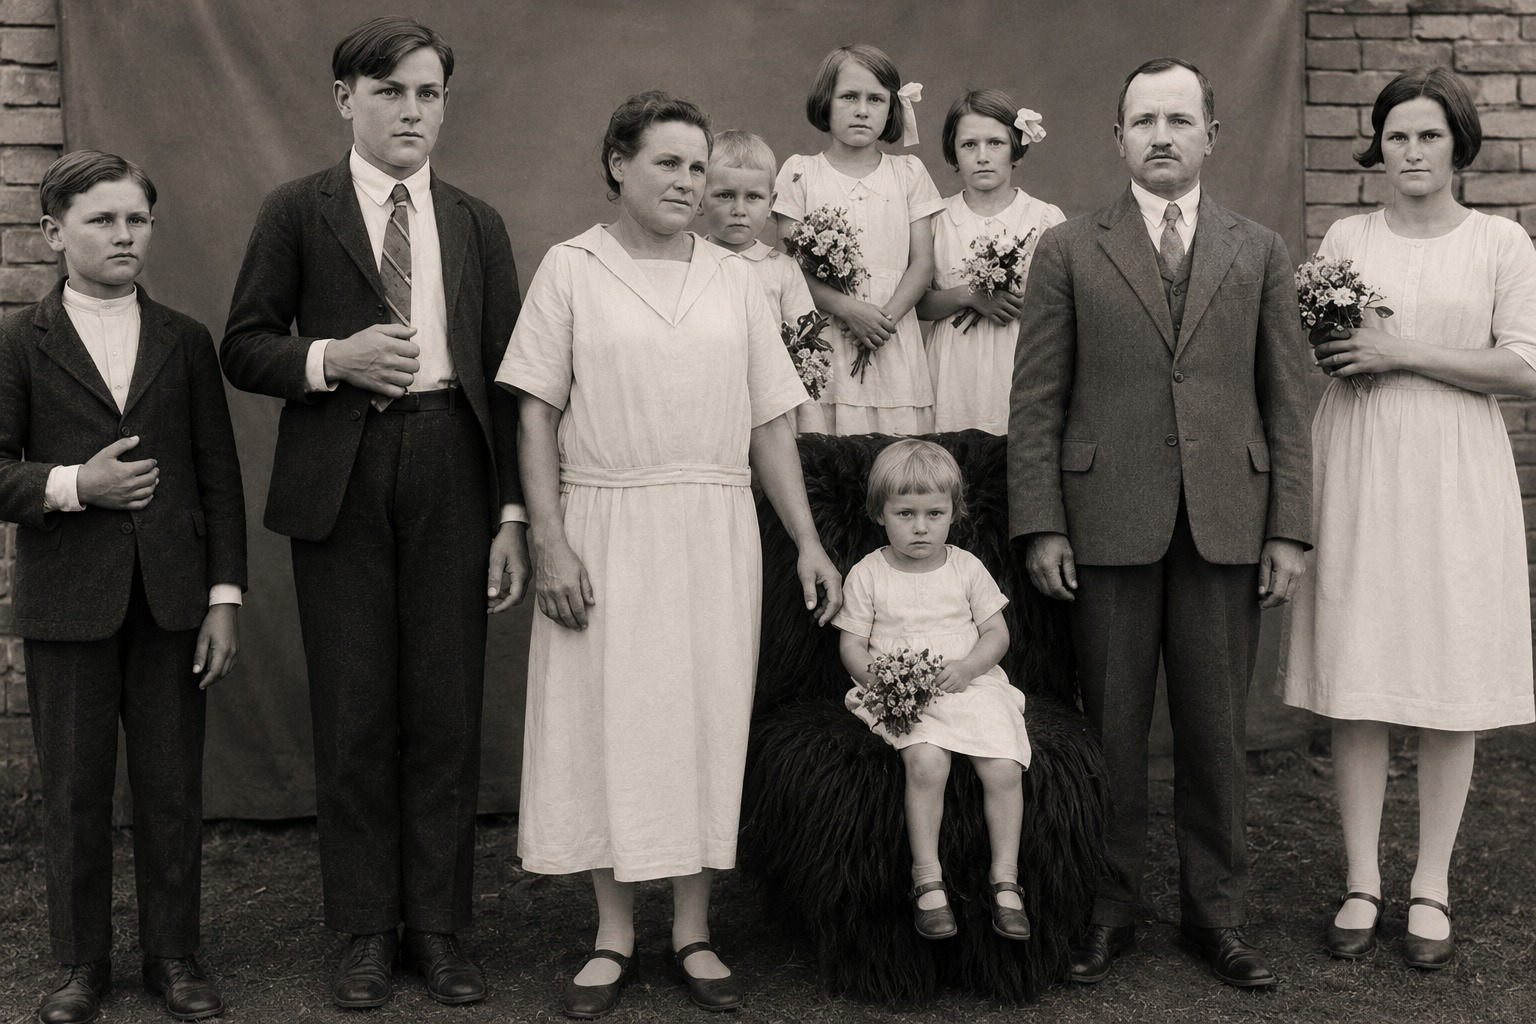
\includegraphics[width=0.85\linewidth,height=\textheight,keepaspectratio,alt={Johann Haas, o Fata (segundo da direita para a esquerda), e Maria Meier Haas, a Mota (ao centro, com o bebê no colo), com os sete filhos criados em Santa Catarina. Pela idade aparente das crianças, a foto deve ser da segunda metade dos anos 1920, já em Ituporanga; a identificação de cada filho ainda precisa ser confirmada com os primos. Acervo da família. Versão restaurada com IA; o original está no repositório, e detalhes dos rostos podem ter sido retocados.}]{imagens/foto_familia_johann_haas_e_maria_meyer_restaurada.jpg}
\caption{Johann Haas, o \emph{Fata} (segundo da direita para a
esquerda), e Maria Meier Haas, a \emph{Mota} (ao centro, com o bebê no
colo), com os sete filhos criados em Santa Catarina. Pela idade aparente
das crianças, a foto deve ser da segunda metade dos anos 1920, já em
Ituporanga; a identificação de cada filho ainda precisa ser confirmada
com os primos. Acervo da família. Versão restaurada com IA; o original
está no repositório, e detalhes dos rostos podem ter sido retocados.}
\end{figure}

O homem de bigode é Johann Haas, o \emph{Fata}. A mulher do centro é
Maria Katharina Meier Haas, a \emph{Mota}. As sete crianças e jovens são
os filhos que eles criaram em Santa Catarina: Gertrudes, Fernando,
Alexandre, Agnes, Elza, Baldoíno e Maria. Um deles é meu pai. O bebê no
colo da mãe deve ser a caçula, Maria, nascida em 1926, o que poria a
fotografia por volta de 1927; a criança sentada na frente poderia ser
meu pai, com três ou quatro anos, vestido de branco como era costume
vestir os meninos pequenos naquele tempo; mas também poderia ser outra
pessoa, e não quero transformar um palpite em legenda. Os dois rapazes
de terno seriam Fernando e Alexandre, e a moça da direita, Gertrudes, a
mais velha. Tudo isso é dedução pela idade aparente. Ainda preciso
sentar com os primos e conferir rosto por rosto.

O que sei com certeza é o que falta na fotografia. Faltam Hildegard e
Frida, as duas primeiras filhas, que morreram na Alemanha antes da
viagem. Faltam Luisa e Walter, que atravessaram o oceano com os pais e
morreram pequenos; onde, as fontes da família não concordam, e essa
discordância fica para o próximo capítulo. E falta João, que ainda não
tinha nascido e que também morreria pequeno. Quando olho para essa foto,
procuro também os ausentes.

\section{\texorpdfstring{O \emph{Fata}}{O Fata}}\label{o-fata}

Os netos o chamavam de \emph{Fata}. Durante a infância, achei que fosse
um apelido, uma dessas palavras inventadas que as crianças pequenas usam
e que a família adota. Demorei a entender que era simplesmente
\emph{Vater}, pai em alemão, pronunciado do jeito que os filhos o
chamavam em casa e ouvido pelos ouvidos brasileiros dos netos. O mesmo
com a \emph{Mota}: \emph{Mutter}, mãe. No texto que minha irmã Marise
escreveria para o centenário da chegada, em 2013, ela usa as duas formas
lado a lado, \emph{Vater (Fata)}, \emph{Mutter (Mota)}, como quem traduz
e ao mesmo tempo preserva. Os netos herdaram dos filhos a palavra
\emph{pai} e a palavra \emph{mãe} e as transformaram em nomes próprios.
Em nenhuma outra família conheço avós chamados assim, e gosto de pensar
que isso diz alguma coisa sobre aquela casa: os filhos falavam tanto com
os pais, e com tanta naturalidade, que a palavra comum virou nome.

Johann Haas nasceu na Baviera em julho de 1884. Vinha de uma família de
pedreiros e se especializou num ofício que hoje quase desapareceu: o
trabalho em gesso. Fazia molduras de janelas, contornos de portais,
ornamentos de altares, tudo aquilo que nas igrejas e nas casas mais
ricas da Europa daquele tempo dava acabamento à alvenaria bruta. Era um
trabalho que exigia mão firme e olho de artista, e que ele traria
consigo para um país onde quase ninguém tinha dinheiro para ornamentos.

No Brasil, essa habilidade o salvou mais de uma vez. Nos primeiros anos,
numa terra seca e ácida no interior de Anitápolis, onde a lavoura mal
dava para comer, foi o gesso que comprou o pão: ele passou a fazer
túmulos de granilite para os cemitérios da região, decorados com
desenhos e com anjos moldados à mão. Mais tarde, em Ituporanga, foi o
ofício de pedreiro que o sustentou, e ele o ensinou aos filhos. A
família construiu, na cidade, a Igreja Matriz, a Casa Paroquial, o
Seminário Franciscano e a ampliação do Hospital das Irmãs. Construiu
também casas, escolas, fornos, fogões, escadarias e serrarias por toda a
região, nem sempre pelas mãos dele, mas pelas mãos de quem tinha
aprendido com ele.

O que mais aparece nas lembranças, porém, é o temperamento.
\emph{``Nosso João era brincalhão e divertido: um piadista''}, escreveu
Marise. Nunca perdia a oportunidade de dizer alguma coisa engraçada. Os
netos que conviveram com ele nos últimos anos, em Ribeirão das Pacas,
contam que gostavam de sentar perto dele para ouvir histórias, sobretudo
depois que ele tinha tomado umas cervejas, quando a língua se soltava e
a Alemanha voltava a aparecer nas conversas.

Era também um homem de leitura. É um detalhe que me comove, talvez por
deformação profissional. Eram imigrantes pobres, como a maior parte dos
que vinham para as colônias, mas, como diz o texto do centenário,
\emph{cultos}. Trouxeram livros da Alemanha, e esses livros foram lidos
e relidos na casa da mata. Mais tarde a família assinava jornais,
principalmente os que vinham da região de Blumenau, onde a imprensa em
língua alemã ainda era forte, para acompanhar as notícias do Brasil e do
país distante. Imagino o \emph{Fata}, à noite, depois de um dia inteiro
de obra, lendo à luz de lampião um jornal de Blumenau com uma semana de
atraso, procurando alguma notícia da Baviera. Não sei se a cena
aconteceu exatamente assim. Sei que algo parecido com ela aconteceu
muitas vezes.

E havia mais uma habilidade, que só fui compreender muito depois e que
se revelaria uma pista. Segundo o texto do centenário, Johann era
chamado com frequência para servir de intérprete, porque dominava vários
dialetos alemães. Hoje, quando se pensa em alemão, pensa-se numa língua
única, a do rádio e dos livros. Mas a Alemanha em que ele nasceu tinha
sido unificada como país havia apenas treze anos, e como língua estava
longe disso. Um camponês da Pomerânia e um camponês da Baviera podiam
ter dificuldade real de se entender. Nas colônias brasileiras, onde se
misturavam imigrantes de todas as regiões, alguém que transitava entre
esses falares era precioso. Era também, para quem investiga, um sinal: o
\emph{Fata} tinha um ouvido treinado para sotaques, e o seu próprio
sotaque dizia de onde ele vinha.

\begin{figure}
\centering
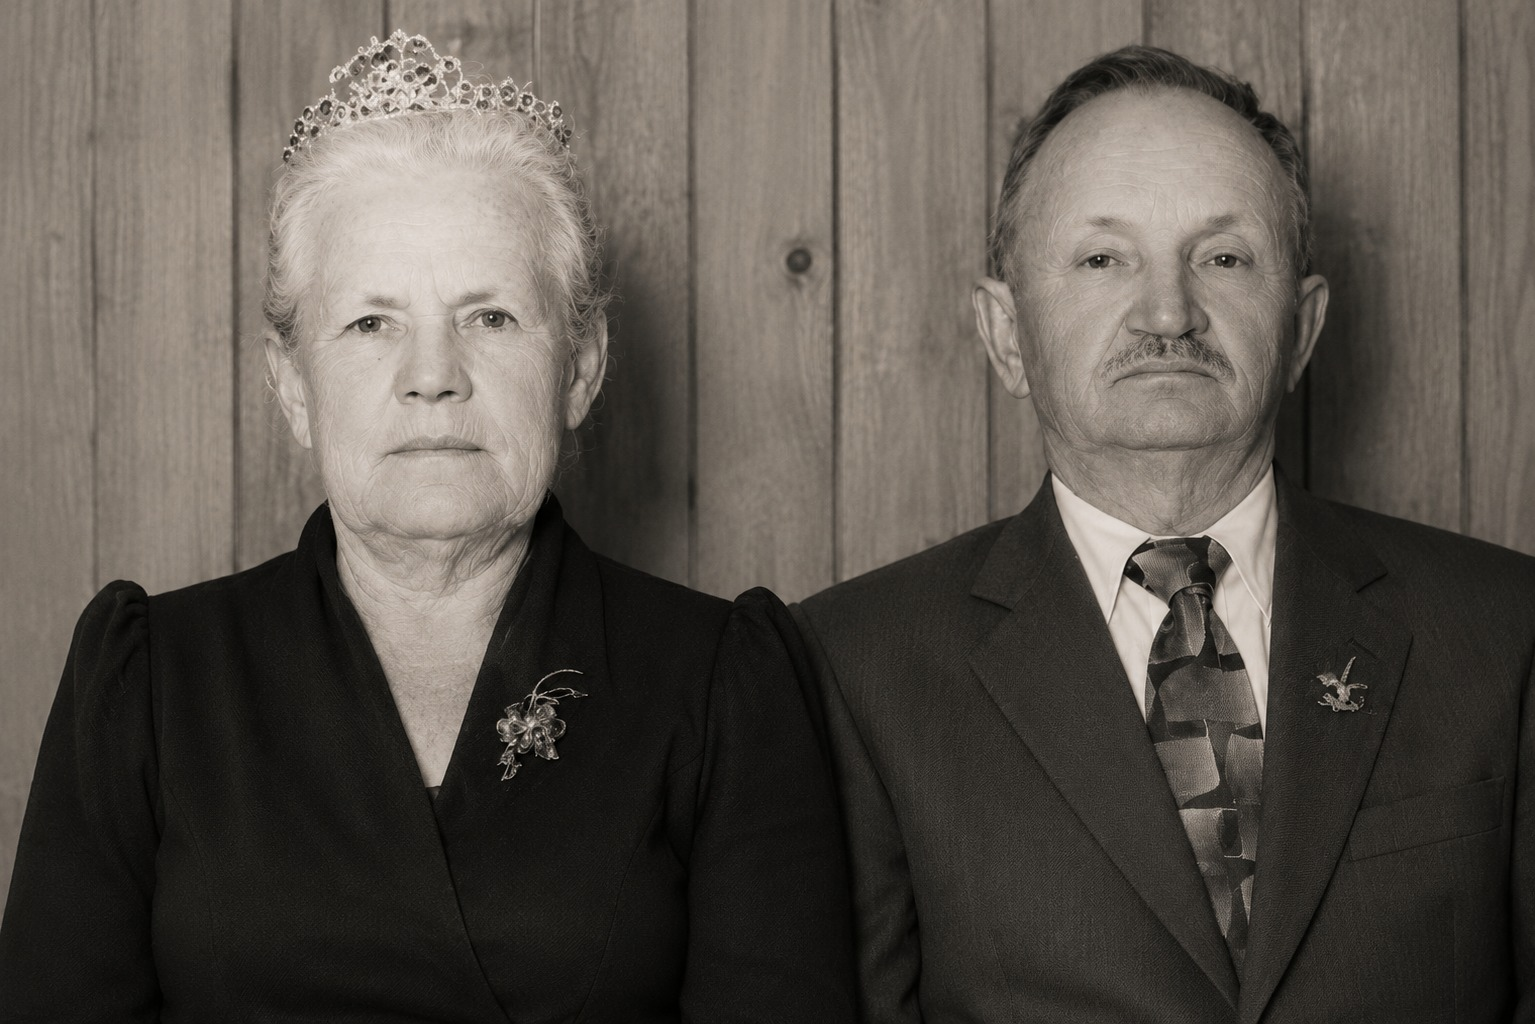
\includegraphics[width=0.75\linewidth,height=\textheight,keepaspectratio,alt={O Fata e a Mota nas Bodas de Ouro, em 1957 pela conta dos cinquenta anos do casamento de 1907: ela com uma pequena tiara no cabelo branco e uma flor presa ao vestido escuro; ele de terno, gravata e um broche na lapela. Acervo da família. Versão restaurada com IA; o original está no repositório, e detalhes dos rostos podem ter sido retocados.}]{imagens/haas_bodas_de_ouro_fata_e_mota_restaurada.jpg}
\caption{O \emph{Fata} e a \emph{Mota} nas Bodas de Ouro, em 1957 pela
conta dos cinquenta anos do casamento de 1907: ela com uma pequena tiara
no cabelo branco e uma flor presa ao vestido escuro; ele de terno,
gravata e um broche na lapela. Acervo da família. Versão restaurada com
IA; o original está no repositório, e detalhes dos rostos podem ter sido
retocados.}
\end{figure}

\section{\texorpdfstring{A \emph{Mota}}{A Mota}}\label{a-mota}

Se o \emph{Fata} era a voz da casa, a \emph{Mota} era o chão.

Maria Katharina Meier nasceu em Heumaden, na Baviera, em abril de 1888.
De que casa ela vinha, só fui saber muito depois. Antes de partir para o
Brasil, além dos trabalhos da casa, ganhava salário ordenhando vacas.
Era ela, segundo a tradição da família, quem conhecia a lida do campo, e
é provável que tenha sido ela o ponto de apoio prático de toda a
aventura: o \emph{Fata} sabia construir paredes, mas quem sabia fazer a
terra produzir, cuidar dos animais e manter uma casa funcionando no meio
do mato era a \emph{Mota}.

Durante os anos em Rio Novo, quando a família morava numa casa pequena
levantada no meio da mata, o \emph{Fata} passava dias e dias na cidade
trabalhando como pedreiro. A \emph{Mota} ficava sozinha com os filhos.
Cuidava da roça, dos animais, das crianças, e, nas palavras do texto do
centenário, defendia-se como podia, com o olhar sempre na estrada,
esperando o marido chegar com os provimentos que a terra não dava. Foi
nessa casa que nasceram Agnes, Elza, meu pai e Maria. Penso nela muitas
vezes quando ouço falar da coragem dos pioneiros. A coragem de enfrentar
o desconhecido costuma ser atribuída a quem parte. Há também a coragem
de quem fica, sozinha, numa clareira, com quatro ou cinco crianças
pequenas, ouvindo os barulhos da noite.

Ela nunca aprendeu o português. O contato com os falantes da língua era
pouco; a vida dela se passava entre a casa, a roça, a família e a
igreja, e em todos esses lugares se falava alemão. Quando os netos
nasceram, muitos deles já sem saber alemão, abriu-se entre a avó e eles
uma distância que nenhuma das partes tinha escolhido. Marise conta que
isso prejudicou muito a comunicação, mas não impediu a \emph{Mota} de
tocar o coração dos netos com olhares, gestos firmes e o que ela chama,
com carinho, de \emph{``resmungões''}. Gosto dessa palavra. Imagino uma
senhora de cabelo branco resmungando em dialeto bávaro para uma criança
que não entende uma palavra e que, mesmo assim, entende tudo.

Nos últimos anos, em Ribeirão das Pacas, a \emph{Mota} caminhava pela
roça apoiada em bengalas feitas de pedaços de pau. Os netos mais
próximos, filhos de Agnes e de Maria, que moravam ali perto, a ajudavam
a segurá-las. São eles que guardam as lembranças mais vivas dela, e são
eles que me fazem falta neste capítulo: preciso ainda ouvir cada um com
calma, com gravador, e pedir licença para citar o que disserem. Por
enquanto, o que tenho é a síntese que Marise fez de muitas vozes, e uma
imagem que se repete em todas elas. A \emph{Mota} abraçava.
\emph{``Nunca perdia a oportunidade de abraçar, abraçar, abraçar''},
escreveu minha irmã. E tinha olhos azuis, que o texto chama de
\emph{infinitamente meigos}.

\begin{figure}
\centering
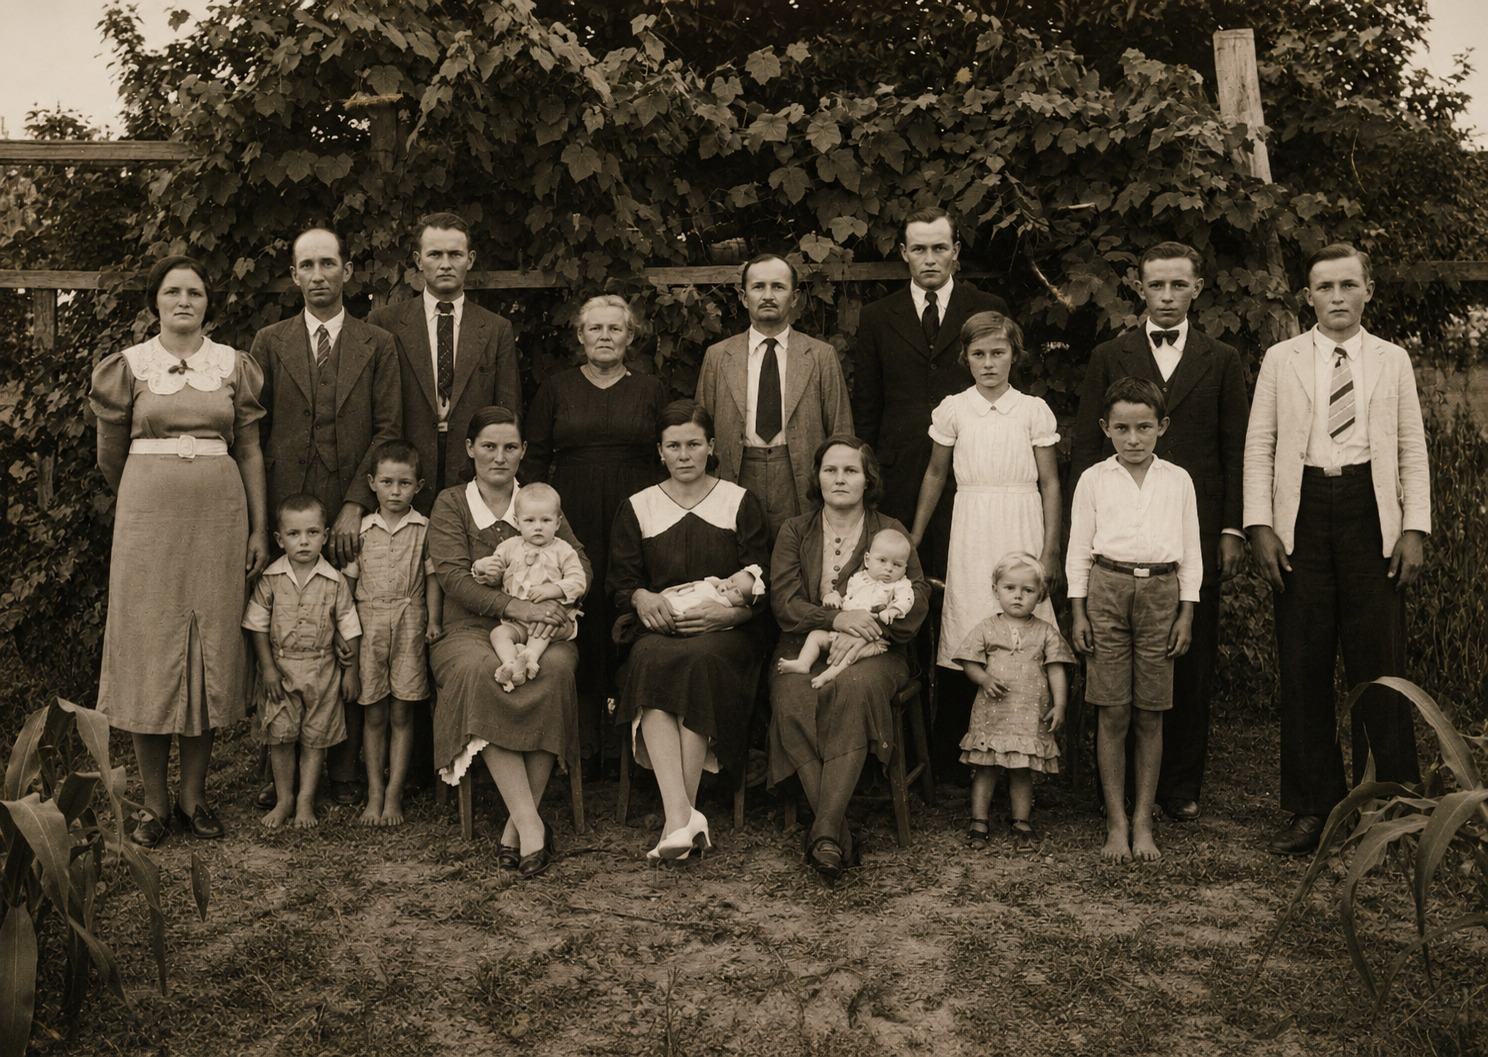
\includegraphics[width=0.85\linewidth,height=\textheight,keepaspectratio,alt={Os primeiros netos do Fata, reunidos com os avós sob uma parreira, provavelmente no fim dos anos 1930. O Fata e a Mota estão no centro da fileira de trás; à frente, três mães sentadas com bebês no colo e crianças descalças em pé. A identificação individual está a confirmar. Acervo da família. Versão restaurada com IA; o original está no repositório, e detalhes dos rostos podem ter sido retocados.}]{imagens/haas_primeiros_netos_do_fata_restaurada.jpg}
\caption{Os primeiros netos do \emph{Fata}, reunidos com os avós sob uma
parreira, provavelmente no fim dos anos 1930. O \emph{Fata} e a
\emph{Mota} estão no centro da fileira de trás; à frente, três mães
sentadas com bebês no colo e crianças descalças em pé. A identificação
individual está a confirmar. Acervo da família. Versão restaurada com
IA; o original está no repositório, e detalhes dos rostos podem ter sido
retocados.}
\end{figure}

Nessa outra fotografia, que a família guarda como a dos primeiros netos,
a \emph{Mota} aparece de vestido escuro, já de cabelos claros, de pé no
meio de filhos, genros, noras e netos, sob uma parreira carregada de
folhas. É a única que olha para a câmera com algo parecido com um meio
sorriso. Ao lado dela, de gravata escura, o \emph{Fata}. As crianças da
frente estão descalças, como as crianças das colônias costumavam andar,
e as mães seguram os bebês com aquele jeito de quem tem prática. Não sei
o nome de todas as pessoas da foto e não vou arriscar. Sei que é uma
fotografia de colheita: vinte e poucos anos depois de chegarem ao Brasil
com duas crianças que não chegariam a crescer, os dois estavam ali,
rodeados de gente que só existia porque eles tinham ficado.

João Haas morreu em 19 de março de 1969, e Maria em 8 de novembro de
1973, ambos com oitenta e cinco anos. Estão sepultados no cemitério de
Aurora, perto de muitos túmulos que ele mesmo fez.

\section{Duas palavras}\label{duas-palavras}

Durante muito tempo, tudo o que a família sabia sobre a origem exata dos
dois cabia em duas palavras.

Do lado da \emph{Mota}, a palavra era \emph{Heumaden}. Do lado do
\emph{Fata}, \emph{Sandberg}, às vezes acompanhada de \emph{Leonberg}.
Eram palavras ditas, mais do que escritas, e mudavam um pouco conforme
quem as dizia. Na planilha que meu primo Agenor montou ao longo de anos,
e da qual falarei no próximo capítulo, a aldeia da \emph{Mota} aparece
grafada \emph{Heimaden}, com \emph{i}, e Johann aparece como nascido
``em Leonberg, que hoje se chama Maxhütte, que fica no estado de
Bayern''. Era muito mais do que eu tinha. Era também, como eu
descobriria, um campo minado.

A diferença entre \emph{Heumaden} e \emph{Heimaden} parece pequena, uma
vogal, mas diz muito sobre como os nomes viajam. Uma palavra transmitida
de boca em boca durante noventa anos, por gente que já não falava a
língua de origem, vai se acomodando ao ouvido de quem a repete.
\emph{Heu} é feno, em alemão; o restante do nome lembra \emph{Mahd}, a
ceifa, o corte do capim, e a aldeia, imagino, deve ter nascido de algum
prado de feno ceifado no verão para alimentar o gado no inverno.
\emph{Heim}, por outro lado, é lar, casa. Não sei se a troca foi de quem
ouviu ou de quem escreveu, nem tenho como saber. Mas não deixo de achar
bonito que, ao passar pela memória de três gerações brasileiras, a
aldeia do feno tenha ficado parecida com a aldeia de casa.

Os nomes das pessoas sofreram o mesmo desgaste. Meier virou Meyer em
muitos papéis brasileiros, e as duas grafias convivem até hoje nos
documentos da família. Johann virou João, e Maria ganhou na memória da
família um Katharina que, no livro de batismos, era o nome da irmã mais
velha. Na planilha, o pai da \emph{Mota} aparece como Adam Meyer e a mãe
como Franciska Meyer, com o sobrenome do marido, como era costume
registrar as mulheres casadas. Cada uma dessas pequenas mudanças é
inocente. Somadas, podem tornar uma pessoa irreconhecível num arquivo do
outro lado do mar.

Para um meteorologista, uma estação de observação é um par de coisas: um
conjunto de medidas e uma posição. As medidas sozinhas não servem para
nada. Uma temperatura de dois graus negativos às seis da manhã é uma
informação banal se a estação estiver no alto de uma serra, e é um
alarme se estiver numa várzea do litoral. Por isso toda estação tem
coordenadas: latitude, longitude, altitude. E por isso um dos erros mais
traiçoeiros que se pode cometer na análise de dados é o erro de
posicionamento: uma medida correta atribuída ao lugar errado. Ela não
parece errada. Os números são plausíveis, o formato é perfeito, nada
chama a atenção. Mas, quando entra no mapa, ela contamina tudo ao redor.
O programa de análise ajusta as isolinhas para acomodar aquele valor, e
o que deveria ser um campo suave ganha uma bolha estranha, um falso
núcleo de frio ou de calor, que pode convencer um previsor desatento de
que há algo ali onde não há nada.

Os nomes de lugares numa genealogia funcionam como as coordenadas de uma
estação. Se estiverem certos, as medidas, as datas, os nomes dos pais,
os ofícios, se encaixam num mapa coerente. Se estiverem errados, tudo o
que vier depois será construído sobre um ponto deslocado. E nomes de
aldeias alemãs são especialmente traiçoeiros, porque se repetem.

\section{O perigo dos homônimos}\label{o-perigo-dos-homuxf4nimos}

Basta digitar as duas palavras num mapa da internet para entender o
problema.

Leonberg, para qualquer alemão e para a maior parte dos mapas, é uma
cidade de Baden-Württemberg, uns quinze quilômetros a oeste de
Stuttgart. É uma cidade conhecida, com centro histórico, castelo, uma
raça de cães gigantes que leva seu nome e uma autoestrada que passa ao
lado. Quem procura ``Leonberg, Alemanha'' cai lá quase sempre. E
Heumaden, por uma coincidência que parece armada de propósito, também
existe nos arredores de Stuttgart: é um bairro da própria cidade, na
zona de Sillenbuch, a uns vinte quilômetros de Leonberg.

Pensem na tentação. Um pesquisador brasileiro, com duas palavras
transmitidas oralmente por quase cem anos, digita os dois nomes e
descobre que ambos existem, lado a lado, na mesma região metropolitana
do sudoeste da Alemanha. Parece um achado. Parece a confirmação de que a
família inteira, \emph{Fata} e \emph{Mota}, vinha de uma mesma área, o
que explicaria como os dois se conheceram. Os dados são plausíveis, o
formato é perfeito, nada chama a atenção. É o erro de posicionamento em
estado puro.

Não vou dizer aqui que caí nessa armadilha, porque não tenho registro de
ter caído, e não quero inventar um tropeço para tornar a história mais
dramática. Mas sei que ela estava armada no caminho, e sei que muitos
pesquisadores de família, no Brasil e fora dele, já perderam meses em
cidades homônimas, consultando arquivos que nunca guardaram um único
papel dos seus antepassados. Os fóruns de genealogia estão cheios dessas
histórias. Por isso dedico a ela algumas linhas: para que vocês, se um
dia continuarem esta pesquisa, saibam que o primeiro resultado do mapa
quase nunca é o certo.

Havia pelo menos três sinais de que a região de Stuttgart não era a
resposta. O primeiro estava na própria nota do Agenor: Leonberg, dizia
ele, ficava em \emph{Bayern}, a Baviera, e tinha mudado de nome para
\emph{Maxhütte}. A Leonberg de Stuttgart nunca foi bávara, nem mudou de
nome. O segundo era a palavra \emph{Sandberg}, que não aparecia em
nenhum mapa perto de Stuttgart. O terceiro era o sotaque.

Os dialetos falados em torno de Stuttgart são suábios, da família
alemânica, aparentados aos falares da Suíça alemã e da Alsácia. Os da
Baviera pertencem a outra família, a bávara, aparentada aos falares da
Áustria. Para um ouvido brasileiro, é tudo alemão. Para um alemão, é a
diferença entre um gaúcho da fronteira e um nordestino do sertão, e às
vezes mais. O título deste capítulo fala em sotaque bávaro, e ele
adianta uma conclusão que só os documentos confirmariam mais tarde. Mas
o raciocínio já estava disponível: se o \emph{Fata}, que transitava
entre dialetos e era chamado justamente para traduzir uns para os
outros, fosse de Stuttgart, teria crescido falando suábio, e a família
guardaria dele outra música. E a única pista escrita que eu tinha, a
nota do Agenor, dizia \emph{Bayern} com todas as letras.

Quando se procura Leonberg dentro da Baviera, aparece outra coisa. No
Alto Palatinado, a \emph{Oberpfalz}, a região do nordeste bávaro que faz
fronteira com a Boêmia, a pouco mais de vinte quilômetros ao norte de
Regensburg, existe um município chamado Maxhütte-Haidhof. O nome vem de
uma siderúrgica, a \emph{Maximilianshütte}, fundada no século XIX, em
torno da qual cresceu uma cidade operária. Leonberg e Sandberg são
localidades que hoje fazem parte desse município. A nota do Agenor
estava certa, e a palavra \emph{Sandberg} se encaixava: era o nome de um
lugarejo ligado a Leonberg, ao lado da siderúrgica, e o lugar onde, ao
que tudo indicava, a família de Johann tinha vivido.

E Heumaden? Também existe na \emph{Oberpfalz}. É uma aldeia pequena do
município de Moosbach, no distrito de Neustadt an der Waldnaab, a menos
de vinte quilômetros da atual fronteira com a República Tcheca, numa
região de colinas, florestas e pequenos lugarejos agrícolas. Fica a
cerca de cinquenta quilômetros em linha reta de Maxhütte-Haidhof, e a
mais de duzentos de Stuttgart. A paróquia que a atende é a de São Pedro
e São Paulo, em Moosbach.

Desenhei os dois pontos no mapa como desenharia duas estações. Duas
aldeias da mesma região, separadas por uma distância que se fazia a pé
em dois dias ou de trem em poucas horas, ambas no Alto Palatinado, ambas
no mesmo dialeto. De repente as duas palavras deixavam de ser lendas e
passavam a ser coordenadas: Heumaden, cerca de 49,6° de latitude norte e
12,4° de longitude leste; Leonberg, em Maxhütte-Haidhof, cerca de 49,2°
norte e 12,1° leste.

Mas havia uma terceira palavra na nota do Agenor que não se encaixava em
nada disso. Segundo ele, Johann e Maria tinham se casado em 3 de agosto
de 1907 em \emph{Eibenstock}. Eibenstock, se for a cidade que os mapas
mostram, não fica na Baviera. Fica na Saxônia, nos Montes Metálicos,
junto à fronteira tcheca, bem mais ao norte. O que um estucador de
Leonberg e uma moça de Heumaden estariam fazendo lá? Trabalho, talvez.
Uma obra, uma temporada, um parente. Ou talvez seja outro homônimo,
outra estação deslocada. Não sei. Deixo o ponto marcado no mapa com um
sinal de interrogação, que é o que se faz com um dado suspeito: não se
apaga, mas também não se confia nele antes de conferir.

Eu tinha agora duas aldeias reais no lugar de duas palavras, uma data de
casamento num lugar intrigante e um punhado de perguntas que nenhuma
conversa de família ia responder: onde estariam os registros de
nascimento, quem eram os pais de Johann e de Maria, se teriam ficado
irmãos na Baviera, se alguém, do outro lado, ainda carregaria o mesmo
sobrenome.

Eram perguntas grandes demais para um homem só, com um computador e
algumas noites livres por semana. A boa notícia era que eu não estava
só. Havia na família, espalhados pelo Brasil, outros curiosos que vinham
juntando peças havia anos, cada um com seu pedaço do quebra-cabeça e
nenhum com o desenho completo.

\section{Para vocês descobrirem}\label{para-vocuxeas-descobrirem-1}

\begin{itemize}
\tightlist
\item
  Qual das crianças da fotografia dos nove rostos é Baldoíno? Sentem com
  os primos e confiram rosto por rosto.
\item
  O Eibenstock da nota do Agenor é mesmo a cidade da Saxônia, ou é outro
  homônimo? E o que um estucador de Leonberg e uma moça de Heumaden
  estariam fazendo lá?
\item
  A troca de \emph{Heumaden} por \emph{Heimaden} foi de quem ouviu ou de
  quem escreveu?
\item
  O que a \emph{Mota} dizia nos seus ``resmungões''? Perguntem aos netos
  que moravam perto dela em Ribeirão das Pacas, filhos de Agnes e de
  Maria.
\end{itemize}

\chapter{A Irmandade dos Primos-Detetives}\label{cap-3}

\emph{27,6° S · 48,5° O, Florianópolis, SC}

\begin{quote}
\emph{Nenhum observador vê a tempestade inteira. A rede vê.}
\end{quote}

Duas pessoas sérias da família escreveram a história da mesma menina, e
não concordam nem no ano nem no continente em que ela nasceu. Para minha
irmã, Gertrudes, irmã do meu pai, nasceu em 5 de maio de 1913 no
Barracão dos Imigrantes de Laguna. Para um primo, nasceu em 22 de
outubro de 1911, ainda na Alemanha, e veio com um ano de idade no
\emph{Formosa}. Cheguei a essa contradição aos poucos.

\section{Cem anos depois}\label{cem-anos-depois}

Em 30 de março de 2013, os descendentes de João e Maria Meyer Haas se
reuniram para comemorar o centenário da chegada dos dois ao Brasil.
Éramos, segundo a conta que se fez na época, mais de seiscentos
descendentes diretos, espalhados por Santa Catarina, pelo Paraná e por
outros cantos do país e do mundo. Uma boa parte estava ali.

Não vou reconstituir a festa. Não tenho notas daquele dia, e as imagens
que circulam na memória são vagas demais para virar cena sem que eu
acabe inventando. O que ficou do centenário, para mim, foi um texto.
Minha irmã mais nova, Marise Haas Lourenço, escreveu e leu naquele dia
uma história de João e Maria, assinada ``Florianópolis, março de 2013''.
Esse texto é, até hoje, a fonte mais completa que a família tem sobre os
dois, e boa parte da Parte II deste livro se apoia nele.

\begin{ficha}

\textbf{Ficha do Arquivo}: \emph{História de João e Maria Meyer Haas},
texto de Marise Haas Lourenço lido no centenário da chegada
(30/03/2013), assinado ``Florianópolis, março de 2013''. Cópia digital
no repositório da família:
\texttt{livro/fontes/historia\_joao\_e\_maria\_marise\_2013.txt}. Fontes
declaradas pela autora: documentos e fotos; pesquisas em arquivos,
museus e bibliotecas; entrevistas; relatos.

\end{ficha}

Li esse texto muitas vezes depois daquele dia, e cada leitura me mostrou
uma coisa diferente. Na primeira, li como neto: uma história comovente,
bem contada, com perdas e conquistas, com a coragem dos avós e a
gratidão dos descendentes. Na segunda, li como pesquisador, e comecei a
sublinhar. Na terceira, li como meteorologista, e percebi que o texto
era, ele mesmo, o produto de uma rede.

Marise abre com uma declaração de método que eu gostaria de ter escrito.
Diz que muitos contribuíram para que a história fosse escrita e que,
para não esquecer ninguém, opta por não mencionar nenhum nome. Diz que o
texto \emph{``não resulta da cabeça de quem escreveu''}, mas tenta se
aproximar o melhor possível da verdade. E lista as fontes: documentos e
fotos, pesquisas em arquivos, museus e bibliotecas, entrevistas,
relatos. Há ali, sem que ela use a palavra, a descrição exata de um
trabalho de síntese: muitas observações parciais, de qualidade desigual,
combinadas num retrato único.

Logo depois, ela faz uma observação que me pareceu, na época, apenas uma
gentileza, e que hoje considero a frase mais importante do texto. A
família Haas, escreve, \emph{``não é um sobrenome''}, mas o conjunto de
inúmeros outros, sem os quais não existe família. E agradece
nominalmente a alguns deles: aos Meyer, da \emph{Mota}; aos Sebold, do
Tio Augusto; aos da Rosa, da Tia Rosalina; aos Klettenberg, da Tia
Paula; aos Boeing, do Tio João; aos Nagel, do Tio Paulo; aos Doerner, da
Tia Adelina, que era minha mãe; e aos Sautner, do Tio Martin. E, por
extensão, a todos os outros sobrenomes sem os quais aquela família de
mais de seiscentos não existiria.

Só fui entender a precisão dessa lista meses depois, quando a comparei
com outra fonte. Mas já na primeira leitura ela me tocou por outro
motivo. Eu tinha passado anos pensando na minha genealogia como uma
linha, a linha Haas, que subia de mim para meu pai, do meu pai para o
\emph{Fata}, do \emph{Fata} para a Baviera. Marise estava dizendo, com
toda a delicadeza, que essa linha não existia sozinha. Que cada geração
tinha sido feita pelo encontro de duas famílias, e que a metade que não
levava o sobrenome era tão responsável pelo resultado quanto a outra.
Era a mesma coisa que eu tinha visto à mesa de Vidal Ramos, entre os
Haas do meu pai e os Doerner da minha mãe. Agora estava escrita.

\begin{figure}
\centering
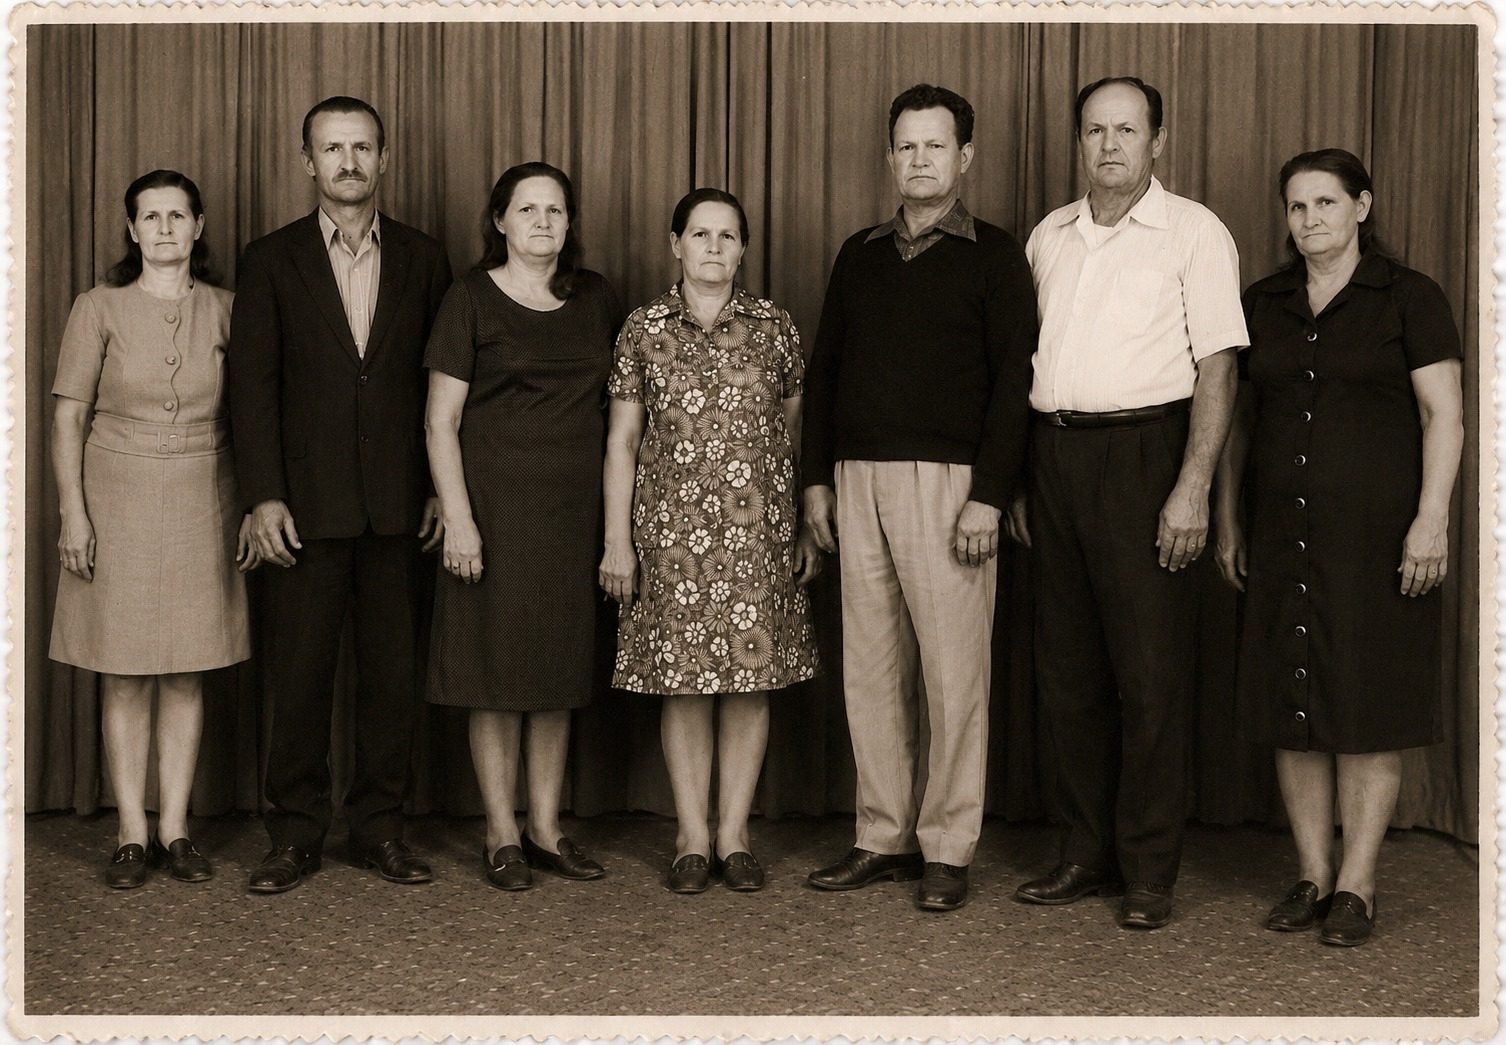
\includegraphics[width=0.85\linewidth,height=\textheight,keepaspectratio,alt={Irmãos Haas reunidos para um retrato de estúdio, diante de uma cortina: quatro mulheres e três homens já maduros, os sete filhos de Johann e Maria que chegaram à idade adulta, entre eles Baldoíno, o meu pai. A data e a posição de cada irmão na foto ainda estão por anotar. Acervo da família. Versão restaurada com IA; o original está no repositório, e detalhes dos rostos podem ter sido retocados.}]{imagens/haas_irmaos_reunidos_restaurada.jpg}
\caption{Irmãos Haas reunidos para um retrato de estúdio, diante de uma
cortina: quatro mulheres e três homens já maduros, os sete filhos de
Johann e Maria que chegaram à idade adulta, entre eles Baldoíno, o meu
pai. A data e a posição de cada irmão na foto ainda estão por anotar.
Acervo da família. Versão restaurada com IA; o original está no
repositório, e detalhes dos rostos podem ter sido retocados.}
\end{figure}

\section{O texto e o que ele não
diz}\label{o-texto-e-o-que-ele-nuxe3o-diz}

O texto de Marise conta a história em ordem. O casamento em 1907, ainda
jovens. O ofício de Johann, de família de pedreiros, especialista em
gesso, intérprete de dialetos. O trabalho de Maria, que ordenhava vacas
por salário. A crise na Alemanha, a ameaça de guerra, a morte precoce
das duas primeiras filhas, Hildegard e Frida, \emph{``por razões que
desconhecemos''}. O nascimento de Luisa em 1910 e de Walter em 1912. A
decisão de partir, tomada, imagina ela, depois de muitas conversas e
muitas opiniões contrárias e favoráveis. O embarque no \emph{Formosa},
em Marselha, com Maria grávida e os dois pequenos no colo.

Depois, a chegada. O texto diz que o navio chegou ao Brasil em 26 de
março de 1913, que o desembarque no Rio de Janeiro foi recusado e que o
vapor seguiu de porto em porto pela costa, cumprindo quarentena, com
excesso de passageiros, comida ruim e higiene precária, e com muitas
mortes a bordo. A família desembarcou finalmente em Laguna, foi levada
para o Barracão dos Imigrantes e ali, seis dias depois, em 5 de maio,
nasceu Gertrudes. Luisa e Walter, enfraquecidos pela viagem, não
resistiram. Quase nada disso, eu descobriria depois, resiste aos
documentos.

Daí em diante, a história segue para o Lote 17 em Rio do Ouro, hoje
Anitápolis, para Ituporanga, Rio Novo, Águas Negras, as obras da cidade,
a guerra, o rádio no porão, a velhice em Ribeirão das Pacas e as
sepulturas em Aurora. Marise não esconde as partes duras. Fala da
política de ocupação das terras indígenas e dos bugreiros pagos por
cabeça, chamando aquilo pelo nome que tem: um genocídio patrocinado pelo
Estado. Fala das notícias de violência contra descendentes de alemães
durante a guerra, que chegavam à família e fizeram o \emph{Fata} manter
a espingarda carregada ao alcance da mão. E termina com uma pergunta que
responde ela mesma: \emph{``Essa parece uma história triste? Não, não é
triste.''}

Como neto, eu concordava. Como pesquisador, comecei a fazer perguntas
que o texto não respondia, nem tinha a obrigação de responder. Em que
data exatamente eles saíram da Alemanha? O desembarque foi mesmo
recusado no Rio? Houve quarentena? Em que porto de Santa Catarina eles
desceram? Onde foram enterrados Luisa e Walter? Se Gertrudes nasceu no
Barracão de Laguna, há um registro de batismo dela na paróquia? E de
onde, na Alemanha, vinham os dois? O texto não dá o nome de nenhuma
aldeia.

Um texto escrito para ser lido num centenário diante de seiscentas
pessoas não é o lugar para notas de rodapé. Eram perguntas que só outros
documentos podiam responder, e eu sabia que alguns desses documentos já
estavam nas mãos de alguém da família.

\section{A planilha de Londrina}\label{a-planilha-de-londrina}

Esse alguém era meu primo-irmão Agenor Haas.

Agenor nasceu em 1943 em Ituporanga, filho mais velho de Alexandre Haas
e Paula Klettenberg, o que faz dele neto do \emph{Fata} e da \emph{Mota}
pelo mesmo caminho que eu, só que vinte e dois anos antes. É engenheiro
civil, formado na Universidade Federal do Paraná, com uma vida dedicada
à execução de obras, e radicado há muitos anos em Londrina. Durante
anos, sem alarde, com paciência de engenheiro e método de quem está
acostumado a orçamentos e cronogramas, montou uma planilha com todos os
descendentes de Johann e Maria que conseguiu encontrar.

Quando a planilha chegou até mim, numa das muitas trocas de mensagens
que tivemos, levei algum tempo para entender o tamanho do que estava
diante de mim. São 291 linhas. Na primeira coluna, os filhos de Johann e
Maria e seus cônjuges; na segunda, os netos; na terceira, os bisnetos;
na quarta, os trinetos. Pelo resumo que acompanha a planilha, são 11
filhos, 63 netos, 194 bisnetos e 109 trinetos. Em muitas células há
comentários, as notas de Agenor, 55 ao todo, com datas, lugares,
profissões e pequenas biografias.

Uma das primeiras coisas que percebi foi que a maior parte daquelas
notas não podia sair do computador. Agenor tinha juntado o que a família
lhe mandava, e a família mandava tudo: endereços completos, números de
telefone, endereços eletrônicos, escolaridade, profissão, situação
conjugal, nomes de crianças. Era um retrato precioso de uma família num
certo momento do início do século XXI, e era também um conjunto de dados
pessoais de pessoas vivas que nunca autorizaram sua publicação. Por isso
nenhum desses dados entra neste livro. Dos descendentes vivos, falo
apenas em números. Das notas, uso só as que tratam dos patriarcas e dos
filhos de Johann e Maria, todos já falecidos ou figuras da história da
família. Se um dia algum primo quiser contar a própria história, que
conte com a própria voz.

As notas dos patriarcas, porém, eram ouro.

Na célula de Johann, Agenor escreveu um pequeno resumo da vida dele. Diz
que era pedreiro, alemão, nascido em Leonberg, \emph{``que hoje se chama
Maxhütte''}, na Baviera, filho de Josef Haas e Franziska. Que casou em 3
de agosto de 1907 em Eibenstock. Que saiu da Alemanha em 13 de março de
1913 e chegou ao Rio de Janeiro em 26 de abril, depois de 44 dias de
viagem, no navio \emph{Formosa}. Que, nas palavras dele, \emph{``não foi
encontrado ainda o registro do desembarque deles em Florianópolis''}.
Que viveu até 1918 em Rio do Ouro, depois em Rio Novo, depois na cidade
de Ituporanga, de novo em Rio Novo, em Águas Negras a partir de 1930 e,
por fim, em Rio das Pacas, Aurora, onde morreu em 19 de março de 1969.
Na célula de Maria, que ela nasceu em 7 de abril de 1888 em
\emph{Heimaden}, filha de Adam e Franciska Meyer, e morreu em 8 de
novembro de 1973.

Era a primeira vez que eu via, por escrito, os nomes dos pais de Johann.
Era a primeira vez que via uma data de casamento. Era a primeira vez que
via a palavra \emph{Maxhütte}. E era também, como logo percebi, a
primeira vez que via a história contada de um jeito diferente do texto
de Marise.

\section{Quando as fontes discordam}\label{quando-as-fontes-discordam}

Coloquei as duas versões lado a lado, como faço quando comparo duas
reanálises da mesma tempestade. Quando dois modelos concordam, a gente
respira aliviado. Quando discordam, é aí que começa o trabalho
interessante, porque a diferença entre eles costuma apontar exatamente
para o lugar onde os dados são mais pobres.

As discordâncias apareceram logo.

A primeira era a data de nascimento de Johann. Agenor escreveu 8 de
julho de 1884. A data que hoje tenho por certa é outra e vem de um
documento que só conto no seu devido lugar. A diferença é pequena,
poucos dias, mas numa investigação genealógica poucos dias podem ser a
diferença entre achar e não achar um registro num livro de cartório.
Naquela altura, eu ainda não tinha como saber qual das datas estava
certa.

A segunda era a data da partida. Agenor dizia 13 de março de 1913. A
família guarda uma fotografia tirada antes da viagem, com uma inscrição
em alemão no verso que diz, traduzida, \emph{``Lembrança! Antes da nossa
partida para o Brasil, 7 de março de 1913''}. Uma foto de despedida pode
ter sido feita alguns dias antes do embarque, e as duas datas não são
necessariamente incompatíveis. Mas eram mais uma peça a encaixar.

A terceira era a chegada. Marise falava em 26 de março de 1913, no Rio
de Janeiro. Agenor falava em 26 de abril, e fazia a conta: 44 dias de
viagem. Fiz a mesma conta e ela fecha: de 13 de março a 26 de abril são,
de fato, 44 dias. A nota de Agenor era coerente consigo mesma. Só que o
dia era o mesmo, 26, e o mês era outro. Tinha todo o jeito de um único
deslize, um mês trocado num papel em algum momento da transmissão, que
depois se propagou para o cálculo dos dias. Era como encontrar, numa
série de dados, um valor perfeitamente consistente com os vizinhos,
salvo por um dígito.

A quarta era a mais séria, e era sobre Gertrudes. Pelo texto do
centenário, ela nasceu em 5 de maio de 1913 no Barracão dos Imigrantes
de Laguna, seis dias depois do desembarque: era o bebê que Maria trazia
no ventre durante a viagem. Pela planilha de Agenor, Gertrudes nasceu em
22 de outubro de 1911, ainda na Alemanha, e veio com um ano de idade no
\emph{Formosa}.

A quinta estava ligada à quarta. No texto de Marise, as duas crianças
que morreram depois da chegada se chamavam Luisa e Walter, nascidos na
Alemanha em 1910 e 1912, e morreram em Laguna. Na planilha de Agenor não
há Luisa nem Walter. Há, em vez disso, uma Lina e um Valter, que teriam
nascido no Brasil, em Rio do Ouro, e morrido pequenos, sepultados em
Anitápolis. Na planilha, os dois aparecem listados entre Alexandre, de
1917, e Agnes, de 1920, como se tivessem nascido nesse intervalo. Há até
um detalhe curioso: a nota de Valter diz que ele \emph{``faleceu ainda
pequena''}, no feminino, como se a frase tivesse sido copiada da nota de
Lina e não corrigida.

Por fim, havia Eibenstock, a cidade do casamento, que não ficava nem
perto de Leonberg nem perto de Heumaden. E havia um detalhe na contagem.
O resumo fala em onze filhos; mas, percorrendo a primeira coluna linha
por linha, encontrei doze nomes, porque o pequeno João, o caçula que
morreu criança, aparece sozinho perto do fim da tabela. Pelo texto de
Marise, também se chega a doze: as quatro crianças perdidas, os sete que
cresceram e João. A diferença, aqui, parece ser apenas de quem conta e
de como conta.

Durante algum tempo achei que teria de escolher entre as duas fontes.
Depois percebi que não era o caso. Nenhuma das duas era um documento
original. Ambas eram sínteses feitas por pessoas sérias, a partir de
memórias e papéis que circulavam na família, e cada uma tinha herdado
erros e acertos de suas próprias fontes. Eu precisava de uma observação
independente.

Ela apareceu na forma de uma lista de passageiros.

\begin{ficha}

\textbf{Ficha do Arquivo}: Lista de passageiros do vapor \emph{Formosa},
procedente de Marselha, assinada ``Rio, le 26 Mars 1913''. Linhas 161 a
164: Haas Johann, 28 anos, casado; Haas Marie, 25 anos, casada; Haas
Luisa, 2 anos; Haas Walter, 1 ano. Todos alemães, agricultores, terceira
classe. Nota ao pé da folha: ``Le Nº 70 continue sur Santos. Restent 174
passagers''. Imagem no repositório:
\texttt{imagens/doc\_haas\_navio\_formosa\_1913.jpg} (reproduzida no
Capítulo 5).

\end{ficha}

O manifesto do \emph{Formosa} é o primeiro documento de fora da família
que encontrei sobre essa história, e por isso o trato com o respeito que
se deve a uma medida direta. Ele confirma várias coisas de uma vez.
Confirma o navio, confirma Marselha, confirma a data de 26 de março de
1913 no Rio de Janeiro, como dizia Marise. Confirma que Johann tinha 28
anos. E confirma que a bordo estavam duas crianças, Luisa, de dois anos,
e Walter, de um.

E não lista nenhuma Gertrudes.

Isso não encerra o caso, mas pesa muito. Se Gertrudes tivesse nascido em
outubro de 1911, estaria a bordo com um ano e meio e, salvo um erro de
registro, apareceria na lista. Mais ainda: Luisa nasceu em 1910 e Walter
em 1912; encaixar entre eles outra criança nascida em outubro de 1911
seria biologicamente possível, mas muito improvável. Gertrudes,
portanto, nasceu depois da viagem. Quando e onde, só descobri muito mais
tarde, e conto no capítulo 5. E o manifesto desmente outra parte da
tradição: os quatro Haas estão vivos na lista assinada no Rio, sem
nenhuma anotação de óbito a bordo. Quanto a Lina e Valter, a hipótese
mais simples é que sejam Luisa e Walter vistos através de várias camadas
de memória: Lina pode ter sido o nome de casa de Luisa, e Valter é
Walter escrito como se pronuncia em português. E aqui Agenor estava mais
perto da verdade do que o texto do centenário: meu pai me contou que foi
com os irmãos a Anitápolis buscar os restos dos irmãos pequenos para
Ituporanga, onde Walter está sepultado. As crianças morreram em Rio do
Ouro, não em Laguna.

O manifesto também deixa suas próprias perguntas. Maria aparece com 25
anos, mas só completaria 25 em abril, depois da chegada; um ano de
diferença, que me lembra que listas de bordo eram preenchidas às
pressas, por funcionários que anotavam o que lhes diziam. E a nota ao pé
da folha, dizendo que um passageiro continuava para Santos e que
restavam 174 a bordo, sugere um navio que seguia distribuindo gente pela
costa, de porto em porto, exatamente como a memória da família conta. A
frase de Agenor sobre o registro do desembarque \emph{``em
Florianópolis''} que nunca foi encontrado ganha outro sentido: talvez
ele não tenha sido encontrado porque o desembarque não foi lá.

E então lembrei da lista de sobrenomes de Marise. Voltei à planilha de
Agenor, à primeira coluna, onde cada filho de Johann e Maria aparece ao
lado do cônjuge, e li os prenomes em ordem: Gertrudes e Augusto;
Fernando, que Agenor grafa Ferdinand, e Rosalina; Alexandre e Paula;
Agnes e João; Elza e Paulo; Baldoíno e Adelina; Maria e Martin. São
exatamente os tios e tias que Marise agradece, na mesma ordem: Tio
Augusto, Tia Rosalina, Tia Paula, Tio João, Tio Paulo, Tia Adelina, Tio
Martin. Duas fontes escritas por pessoas diferentes, em cidades
diferentes, sem que uma tivesse sido feita para conferir a outra, e que,
nesse ponto, se encaixavam como peças cortadas pela mesma serra. Foi a
primeira vez, nesta pesquisa, que senti o prazer muito particular de ver
duas observações independentes concordarem.

\section{A rede}\label{a-rede}

Há um instrumento meteorológico que acho especialmente bonito: a
radiossonda. É uma pequena caixa com sensores de temperatura, umidade e
pressão, presa a um balão de látex cheio de gás. Duas vezes por dia, no
mesmo horário, em centenas de estações espalhadas pelo planeta, alguém
solta um desses balões. Ele sobe por cerca de uma hora e meia,
transmitindo dados por rádio, até estourar a mais de vinte quilômetros
de altura. Cada sondagem, sozinha, conta pouca coisa: o perfil vertical
da atmosfera num único ponto, num único instante. Mas quando se juntam
as sondagens de todas as estações, feitas à mesma hora, aparece o
retrato tridimensional da atmosfera inteira.

Foi isso que aconteceu com a família a partir de 2013. Marise tinha seu
pedaço, feito de entrevistas e relatos. Agenor tinha o dele, feito de
anos de correspondência com os ramos espalhados pelo Paraná e por Santa
Catarina. Eu tinha as memórias de Vidal Ramos, a gravação de minha mãe,
as fotografias. Outros primos tinham outras coisas: uma certidão
guardada numa gaveta, um nome lembrado por uma tia, uma fotografia sem
legenda. Ninguém tinha o desenho completo. Juntos, começávamos a ter um
mapa.

Nessa fase, tratei a família como trato um banco de dados. Deformação
profissional. Passei a guardar cada informação nova com a fonte de onde
veio, cada data com quem a tinha dado, cada divergência anotada ao lado
da versão concorrente. Quando a correspondência com os primos ficou
grande demais para ser acompanhada à mão, escrevi um pequeno programa em
Python que vasculha minha caixa de correio atrás das mensagens sobre
genealogia e as organiza num arquivo só, com data, remetente e anexos,
para que nada se perca numa pasta esquecida. É um programa modesto,
desses que um aluno de graduação escreveria numa tarde, mas me poupou
muitas noites.

Mais tarde, a árvore foi para o FamilySearch, a grande base genealógica
colaborativa mantida pela Igreja de Jesus Cristo dos Santos dos Últimos
Dias, onde qualquer pessoa pode acrescentar ou corrigir um parente,
desde que cite a fonte. A vantagem é enorme: a árvore deixa de ser minha
e passa a ser de todos os que quiserem cuidar dela. A desvantagem
também: qualquer erro, uma vez lançado, se espalha. Ali, a dúvida sobre
o nascimento de meu pai aparece em pequena escala, porque um registro o
dá como nascido em Rio Novo de Águas Mornas, e não no Rio Novo de
Ituporanga. Mais um homônimo à espreita, agora dentro de Santa Catarina.
De tempos em tempos, outro programa, também em Python, baixa da base a
parte da árvore que me interessa e a salva num arquivo no formato que os
genealogistas usam para trocar dados, o GEDCOM. No último que gerei, a
árvore direta de Matheus e Lucas tinha cerca de trinta pessoas, mais de
duzentas fontes citadas e cinquenta e oito pares de coordenadas
geográficas, de aldeias alemãs a cemitérios catarinenses.

O curioso é que, quanto mais eu tratava a família como dados, mais os
dados insistiam em virar gente. Uma data de óbito de 1913 numa célula de
planilha é um número. A mesma data, quando se descobre que é a de uma
menina de dois anos que atravessou o oceano no colo da mãe e não
sobreviveu aos primeiros meses no Brasil, já não cabe numa célula. A
divergência entre Luisa e Lina, que comecei tratando como um problema de
consistência, terminou como uma pergunta sobre o nome que uma mãe usava
para chamar a filha.

\section{Para onde apontam as setas}\label{para-onde-apontam-as-setas}

Ao fim dessa fase, que se estendeu por alguns anos, a rede tinha chegado
a uma conclusão que nenhum de nós formulou de uma vez, mas que todos
fomos aceitando aos poucos.

Do lado brasileiro, havia muito a fazer ainda: procurar o registro de
nascimento de Gertrudes e os óbitos de Luisa e Walter em Anitápolis,
conferir os livros de terras de Anitápolis e os registros do cemitério
de Ituporanga, datar as obras de Ituporanga. Mas as perguntas que mais
nos intrigavam não seriam respondidas aqui. Quem eram Josef Haas e
Franziska, os pais de Johann? Quem eram Adam e Franziska, os pais de
Maria? Em que dia, exatamente, Johann nasceu? Teriam ficado irmãos na
Alemanha? Haveria ainda, em Leonberg ou em Heumaden, alguém com o mesmo
sangue?

Essas respostas não estavam no FamilySearch, nem na planilha de Agenor,
nem no texto de Marise, nem na minha caixa de correio. Estavam em
livros. Livros de registro civil de um pequeno cartório bávaro, livros
de batismo e de casamento de uma paróquia católica do Alto Palatinado,
escritos à mão, em letra gótica, por funcionários e padres mortos havia
mais de um século. Alguns desses livros, talvez, digitalizados em algum
arquivo diocesano. Outros, quase certamente, só consultáveis de corpo
presente, num balcão, diante de alguém disposto a abri-los.

Não sei precisar quando essa conclusão deixou de ser uma frase e virou
uma ideia. Não houve cerimônia. Foi só a constatação, numa das muitas
noites diante da tela, de que todas as setas do meu mapa apontavam para
o mesmo lugar, do outro lado do oceano, e de que nenhuma delas ia chegar
lá sozinha. Se eu quisesse saber o que havia no fim daquelas linhas,
alguém teria de ir até lá.

Ainda faltavam alguns anos para essa viagem. Antes dela, porém, este
livro precisa fazer o que a rede de primos me ensinou: voltar no tempo e
contar a história do jeito que os documentos e as memórias permitem, com
as dúvidas à mostra. Começando um pouco antes de 1913 e do cais de
Marselha, numa aldeia operária da Baviera, à sombra de uma siderúrgica,
num dia de julho de 1884.

\section{Para vocês descobrirem}\label{para-vocuxeas-descobrirem-2}

\begin{itemize}
\tightlist
\item
  Quem Marise ouviu para escrever o texto do centenário? Ela preferiu
  não citar nenhum nome. Perguntem a ela, que é tia de vocês, e aos
  primos mais velhos.
\item
  Quem contou a Agenor o nome \emph{Lina}? Luisa era chamada assim em
  casa, ou esse nome veio de outro lugar?
\item
  Em que ano os irmãos foram buscar os restos das crianças em
  Anitápolis? Walter está sepultado em Ituporanga; e Luisa, onde está?
  Procurem nos óbitos de Anitápolis e nos registros do cemitério de
  Ituporanga.
\item
  Em que porto de Santa Catarina os Haas desceram, se o registro do
  desembarque nunca apareceu em Florianópolis?
\end{itemize}

\part{O Vapor Formosa e a Floresta}\label{o-vapor-formosa-e-a-floresta}

\begin{boletim}

Deslocamento previsto: Marselha, Rio de Janeiro, Laguna. Mar de través,
quarentena prolongada. Na serra, mata fechada e promessas que não se
cumprem.

\end{boletim}

\chapter{Antes da Partida: Das Rodas de Heumaden à Fumaça de
Leonberg}\label{cap-4}

\emph{49,2° N · 12,1° L, Maxhütte-Haidhof · 49,6° N · 12,4° L, Heumaden,
Baviera}

\begin{quote}
\emph{Toda frente fria tem uma origem que ninguém vê: um pedaço de ar
que, um dia, ficou parado tempo demais no mesmo lugar.}
\end{quote}

Segundo a anotação do primo Agenor, Johann e Maria, dois católicos da
Baviera, casaram-se em 3 de agosto de 1907 em Eibenstock. Se é a
Eibenstock que eu conheço dos mapas, ela fica na Saxônia, que era
majoritariamente luterana. O que os dois foram fazer lá? Para chegar a
essa pergunta, preciso começar de onde cada um deles veio.

\section{Duas horas da madrugada em
Heumaden}\label{duas-horas-da-madrugada-em-heumaden}

\emph{Heumaden, Alto Palatinado, 7 de abril de 1888}

Imagino que a parteira tenha vindo a pé. Em abril, no Alto Palatinado,
as estradas de terra ainda guardam a umidade do degelo, e uma carroça
faria mais barulho do que a ocasião pedia. Ela se chamava Glas (é tudo o
que o livro paroquial diz sobre ela: um sobrenome e uma função,
\emph{Hebamme}), e é provável que conhecesse cada casa da aldeia pela
porta da cozinha. Heumaden não era grande: um punhado de casas de pedra
e madeira, alguns celeiros, campos ondulados que descem em direção às
florestas escuras da fronteira com a Boêmia. A igreja ficava em
Moosbach, a paróquia de São Pedro e São Paulo, e era para lá que se
levavam os recém-nascidos, os noivos e os mortos.

Às duas horas da madrugada daquele 7 de abril, na casa do \emph{Ökonom}
Georg Adam Meier, nasceu uma menina. A mãe, Franziska Voit, tinha vinte
e seis anos; o pai, vinte e nove. Casados havia pouco mais de três anos
(a cerimônia fora em 23 de novembro de 1884, na mesma igreja de
Moosbach), já tinham batizado, em junho de 1886, uma menina chamada
Maria Katharina. A recém-nascida de 1888 recebeu só o nome de Maria. A
família sempre a chamou de Maria Katharina, e o livro de batismos sugere
de onde veio a confusão: o nome pertencia à irmã mais velha. Se aquela
primeira menina morreu pequena, como tantas, o livro de óbitos de
Moosbach ainda não nos disse. Foi batizada no mesmo dia, como se fazia
na Baviera católica; a madrinha, diz o livro da paróquia, foi Katharina
Reichenberger, lavradora de Burgtreswitz, a aldeia da mãe. Foi ela a
madrinha de todas as meninas do casal.

Escrevo estas linhas com uma liberdade que vocês, Matheus e Lucas,
precisam conhecer. Eu não sei se chovia naquela madrugada. Não sei se a
parteira veio a pé, se havia lamparina acesa, se o pai esperou na
cozinha ou no curral. O que sei vem de um livro escrito à mão em letra
gótica, que só vou abrir de verdade mais adiante, quando contar a viagem
de inverno de 2018. Por ora, basta dizer que os fatos estão lá: o dia, a
hora, o nome da parteira, a profissão do pai. O resto é o que um
meteorologista faz quando tem uma única estação de observação e precisa
desenhar o mapa inteiro: interpola, com cuidado, sabendo que pode errar.

Uma coisa posso afirmar com alguma segurança, porque é climatologia e
não genealogia: as madrugadas de início de abril naquela parte da
Baviera são frias. O Alto Palatinado fica no coração do continente,
longe do Atlântico que amacia os invernos da Renânia. Quando o
anticiclone se instala sobre a Europa Central e o ar seco desce do
leste, por cima das montanhas da Boêmia, a temperatura despenca durante
a noite. Os camponeses tinham nome para esse vento que vinha da
fronteira: \emph{Böhmischer Wind}, o vento boêmio, frio, persistente,
que seca a pele e congela as poças. Gosto de pensar que a primeira coisa
que a Mota respirou neste mundo foi um pouco desse ar continental, o
mesmo ar que, setenta e tantos anos depois, ela diria aos netos, num
alemão que eles mal entendiam, que nunca mais tinha sentido.

O pai de Maria, Georg Adam, era filho de Michael Meier, que em Heumaden
exercia o ofício de \emph{Wagner}. A palavra não tem tradução exata em
português; \emph{Wagner} é o que faz \emph{Wagen}, carroças, e sobretudo
as rodas das carroças. Era um ofício de precisão: escolher a madeira,
curvá-la, encaixar os raios no cubo, ajustar o aro de ferro aquecido
que, ao esfriar, aperta a roda inteira como um abraço. Georg Adam
aprendeu o ofício do pai e, ao casar, aparece também como \emph{Ökonom},
palavra que nos registros bávaros quer dizer agricultor. A mãe,
Franziska, vinha de Burgtreswitz, aldeia vizinha, filha de Johann Voit,
\emph{Bauer}, camponês proprietário, e de Barbara Woppmann.

Depois de Maria, o livro de batismos de Moosbach registra mais dois
filhos do casal: Theresia, em junho de 1890, e Michael, em abril de
1892, nascido no dia em que Maria fazia quatro anos. Nos quatro
batismos, o pai muda de ofício: \emph{Wagner} em 1886, \emph{Ökonom} em
1888, \emph{Krämer} (pequeno vendeiro) em 1890, \emph{Häusler} (morador
sem terra de lavoura) em 1892. É uma família descendo a escada, num
lugar onde a terra não se multiplicava. Guardem essa frase, porque ela é
a chave deste capítulo inteiro.

E depois de 1892 o livro se cala. Nenhum outro batismo, casamento ou
óbito daquela casa aparece em Moosbach, enquanto os tios e primos que
ficaram em Heumaden seguem enchendo páginas até 1935. Para onde foram
Georg Adam, Franziska e os filhos? A resposta, como vocês vão ver no
Capítulo 7, estava numa gaveta da família, escrita por uma das irmãs da
Mota.

As árvores colaborativas da internet dão a Maria outros irmãos (Johann
Baptist, Barbara, Margaretha, Josef, Georg, Anna), mas nenhum deles
aparece no livro de batismos de Moosbach com estes pais. Ou nasceram em
outro lugar, depois de 1892, ou são de outra família Meier. Fica a
pergunta.

\begin{figure}
\centering
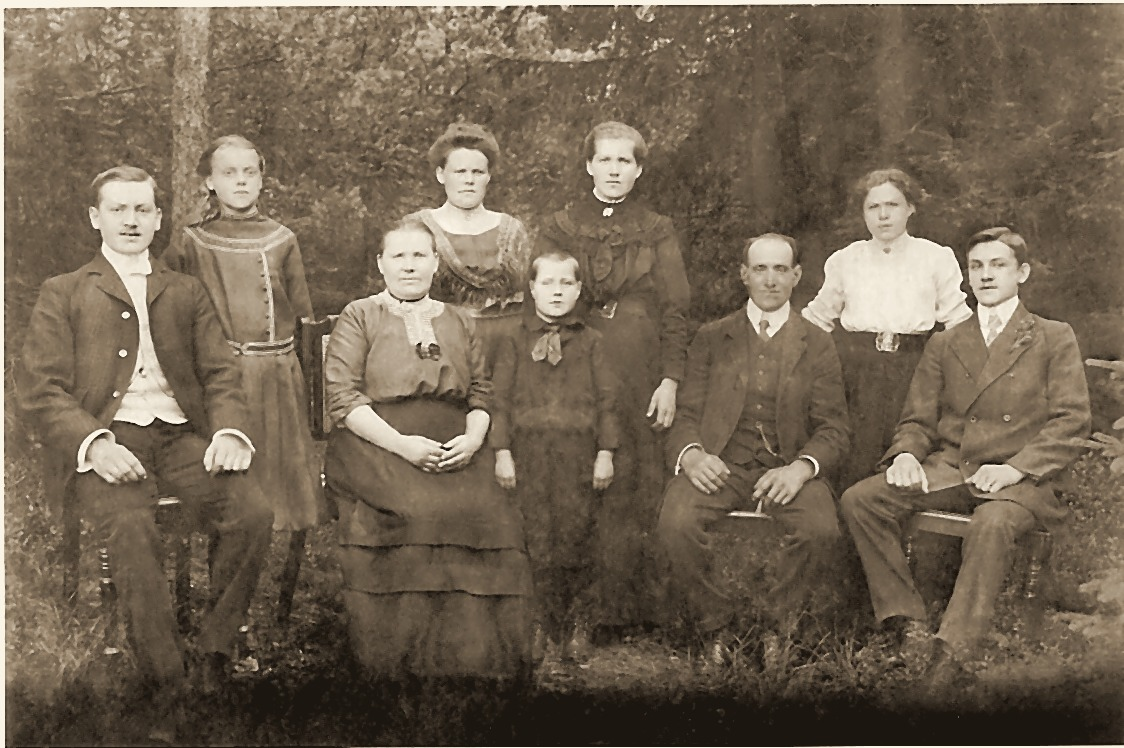
\includegraphics[width=0.85\linewidth,height=\textheight,keepaspectratio,alt={A família da Mota na Alemanha, antes da partida de 1913. Acervo da família; a identificação de cada pessoa ainda está por confirmar. Contraste e tons corrigidos.}]{imagens/meier_familia_da_mota_alemanha_restaurada.jpg}
\caption{A família da Mota na Alemanha, antes da partida de 1913. Acervo
da família; a identificação de cada pessoa ainda está por confirmar.
Contraste e tons corrigidos.}
\end{figure}

\section{O oleiro que não era
nosso}\label{o-oleiro-que-nuxe3o-era-nosso}

\emph{Stoffen, Alta Baviera, 1847, e Leonberg, Alto Palatinado, 1878}

Nas primeiras versões deste livro, o outro lado da história começava
numa aldeia chamada Stoffen, perto de Landsberg am Lech, na Alta
Baviera, quase trezentos quilômetros a sudoeste de Heumaden. As árvores
da internet diziam que Josef Haas, o pai do Fata, tinha nascido ali em
19 de maio de 1847, filho de Georg Haas, um \emph{Ziegelknecht}, peão de
olaria, e de Maria Anna Albrecht. Achei o batismo, li a palavra
\emph{Ziegelknecht}, gostei dela e escrevi páginas sobre o barro de
Stoffen, o gesso de Sandberg e o prumo de Ituporanga, como se fossem
três gerações do mesmo ofício.

Era um homônimo. Joseph Haas é um nome comum na Baviera católica, e o
batismo de Stoffen é verdadeiro, mas é de outro Joseph. Quem desfez o
engano foi o livro de casamentos de Leonberg. Em 4 de março de 1878 (o
ato civil fora em 1º de março), o padre registrou o casamento de
\emph{Haas Joseph}, solteiro, \emph{Fabrikarbeiter} em Leonberg, com
Franziska Dengler, filha de mineiro. Na coluna dos pais do noivo está
escrito, com todas as letras, \emph{Mich. Haas} e \emph{Kunigunde
Stadelmann}. Não Georg e Maria Anna. O avô do Fata se chamava Michael.

\begin{ficha}

\textbf{Ficha do Arquivo}: Paróquia de Leonberg (Diocese de Regensburg),
livro de casamentos 1874--1919 (Matricula: \texttt{Leonberg\_Bul012}),
p.~8, ano 1878, registro nº 4, de 4 de março. Noivo: Joseph Haas,
solteiro, \emph{Fabrikarbeiter} em Leonberg; pais: \emph{Mich. Haas} e
\emph{Kunigunde Stadelmann}. Noiva: Franziska Dengler, de Plattenhof,
filha de Margaretha Dengler, depois casada Rockinger. A leitura dos pais
do noivo foi feita pelo Antigravity e conferida por mim na imagem. O
lugar de origem dos pais, que o Antigravity lê como Etzgersrieth, ainda
não conferi.

\end{ficha}

E aqui vem a parte que me fez largar a caneta. Segundo a leitura do
Antigravity, que ainda preciso conferir com os meus olhos, Michael Haas
e Kunigunde Stadelmann eram de Etzgersrieth, uma aldeia da paróquia de
Moosbach, a uns quatro quilômetros de Heumaden. Se isso se confirmar, a
frase que escrevi mais adiante neste capítulo, de que entre as famílias
do Fata e da Mota havia cinquenta quilômetros, perde o sentido. Os avôs
dos dois teriam ido à mesma igreja de São Pedro e São Paulo, batizado os
filhos na mesma pia e enterrado os mortos no mesmo cemitério. Johann e
Maria podem ter sido, antes de noivos, filhos de vizinhos.

Guardo essa história do oleiro de Stoffen aqui, em vez de apagá-la,
porque ela ensina uma coisa que vale para toda a pesquisa de vocês: um
nome igual e uma data plausível não fazem uma pessoa. É preciso conferir
os pais, o cônjuge, o lugar. Eu não conferi, e passei anos chamando de
trisavô um homem que nunca foi nosso.

A pergunta que o \emph{Ziegelknecht} me fez, porém, continua de pé,
porque vale para os Haas verdadeiros: por que tanta gente da nossa
família, dos dois lados do oceano, trabalhou com as mãos em coisas que
não eram suas?

A resposta mais honesta que encontrei passa pela herança. Na Baviera
antiga (a Alta Baviera, o Alto Palatinado de Heumaden), a terra
camponesa não se dividia entre os filhos. Vigorava, pelo costume e
muitas vezes pela lei, o que os alemães chamam de \emph{Anerbenrecht}: o
direito do herdeiro único. A propriedade passava inteira a um filho, em
geral o mais velho ou o mais novo, conforme o lugar. Os outros recebiam,
quando muito, uma compensação em dinheiro, um enxoval, o direito de
morar na casa enquanto solteiros. A lógica era a da sobrevivência do
sítio: uma fazenda retalhada a cada geração deixa de alimentar quem quer
que seja. Na Renânia e no Mosela, de onde vieram os antepassados da
minha mãe, a regra era o oposto (a partilha igualitária, que picava a
terra em faixas cada vez mais estreitas), e vou contar essa outra
história nos capítulos da Parte III. Os dois sistemas tinham o mesmo
efeito final: empurravam gente para fora da terra.

Na Baviera, o irmão que não herdava tinha poucos caminhos. Podia ficar
como peão na propriedade do irmão. Podia aprender um ofício, e os
ofícios eram, em boa parte, os do barro, da pedra, da madeira e do
ferro. Podia ir para a cidade, para as fábricas que começavam a surgir
no meio do século. Ou podia emigrar. Não sei se Michael Haas era um
filho que não herdou. Sei que o filho dele, Joseph, não ficou na terra:
foi para a fábrica.

Não pretendo, aqui, transformar tudo em teoria. Volto ao assunto da
herança no capítulo 15, onde ele merece mais espaço. Só peço que vocês
notem o padrão, porque ele se repete: o ferro de Sandberg, o gesso do
Fata, o prumo de Ituporanga. Gerações de homens Haas sustentaram suas
famílias construindo coisas que outros iam habitar.

\section{A fumaça da
Maximilianshütte}\label{a-fumauxe7a-da-maximilianshuxfctte}

\emph{Sandberg, perto de Leonberg, Alto Palatinado, julho de 1884}

Em algum momento da juventude (não sei quando, nem por quê), Josef Haas
foi parar em Sandberg, junto de Leonberg, a pouca distância de
Regensburg. Ali havia, desde meados do século, uma usina siderúrgica: a
\emph{Maximilianshütte}, a ``fundição de Maximiliano'', batizada em
homenagem ao rei Maximiliano II da Baviera. A usina deu nome, mais
tarde, ao próprio município: Maxhütte-Haidhof, que hoje engloba Leonberg
e Sandberg. É o caso raro de uma cidade que se chama como a sua fábrica.

Gosto de imaginar o que ele encontrou ali: os altos-fornos, que derretem
o minério de ferro com carvão e ar soprado, num fogo que nunca se apaga.
Uma siderúrgica do século XIX tinha cheiro, barulho e fumaça; o céu, nos
dias de inversão térmica, devia ficar baixo e acinzentado, com a fumaça
das chaminés presa sob uma tampa de ar frio. Conheço bem esse fenômeno:
é o mesmo que, nas manhãs de inverno do Vale do Itajaí, segura a neblina
no fundo dos vales até o sol esquentar o suficiente para rompê-la.

Nos documentos, Josef aparece como \emph{Fabrikarbeiter}, operário de
fábrica. Casou-se com Franziska Dengler. E em 11 de julho de 1884, às
cinco horas da tarde, nasceu em Sandberg o filho que eles chamaram de
Johann, o meu bisavô, o homem que os netos brasileiros chamariam de
Fata. Dois dias depois, em 13 de julho, Josef foi ao cartório civil de
Leonberg declarar o nascimento. O registro recebeu o número 47 daquele
ano.

Há aqui uma pequena divergência que preciso registrar, porque o livro
inteiro é feito de divergências honestamente anotadas. O primo Agenor,
na planilha que é a espinha dorsal da nossa genealogia, escreveu que
Johann nasceu em ``08 de julho de 1884''. O registro civil diz 11 de
julho. Fico com o registro, feito dois dias depois do parto pela boca do
próprio pai. Agenor trabalhou com o que tinha (memória de família,
documentos brasileiros que repetiam a informação de documentos
anteriores), e uma diferença de três dias, depois de um século e um
oceano, é quase um elogio à precisão dele.

Johann não foi filho único. A planilha do Agenor lhe dá os irmãos Josef,
Alois, Georg, Maria, Franziska e Therese. O Antigravity, lendo página
por página os livros de batismo de Leonberg, encontrou outra lista de
filhos de Joseph Haas e Franziska Dengler: Barbara (1879), Joseph
(1880), Kunigunda (1882), Johann (1884), Franz Xaver (1888, morto com
doze dias), Georg (1889) e Sebastian (1891). As duas listas só concordam
em Josef e Georg. Ainda não conferi essas páginas, e por isso deixo as
duas aqui, lado a lado. Uma família operária numerosa, numa vila de
fábrica. Nenhum desses irmãos aparece no Brasil.

Há um detalhe nessa leitura que, se for confirmado, resolve outra
pergunta. O livro de batismos de Leonberg daria o nascimento de Johann
em 8 de julho de 1884, e não em 11. Seria de lá que veio a data do
Agenor.

\begin{figure}
\centering
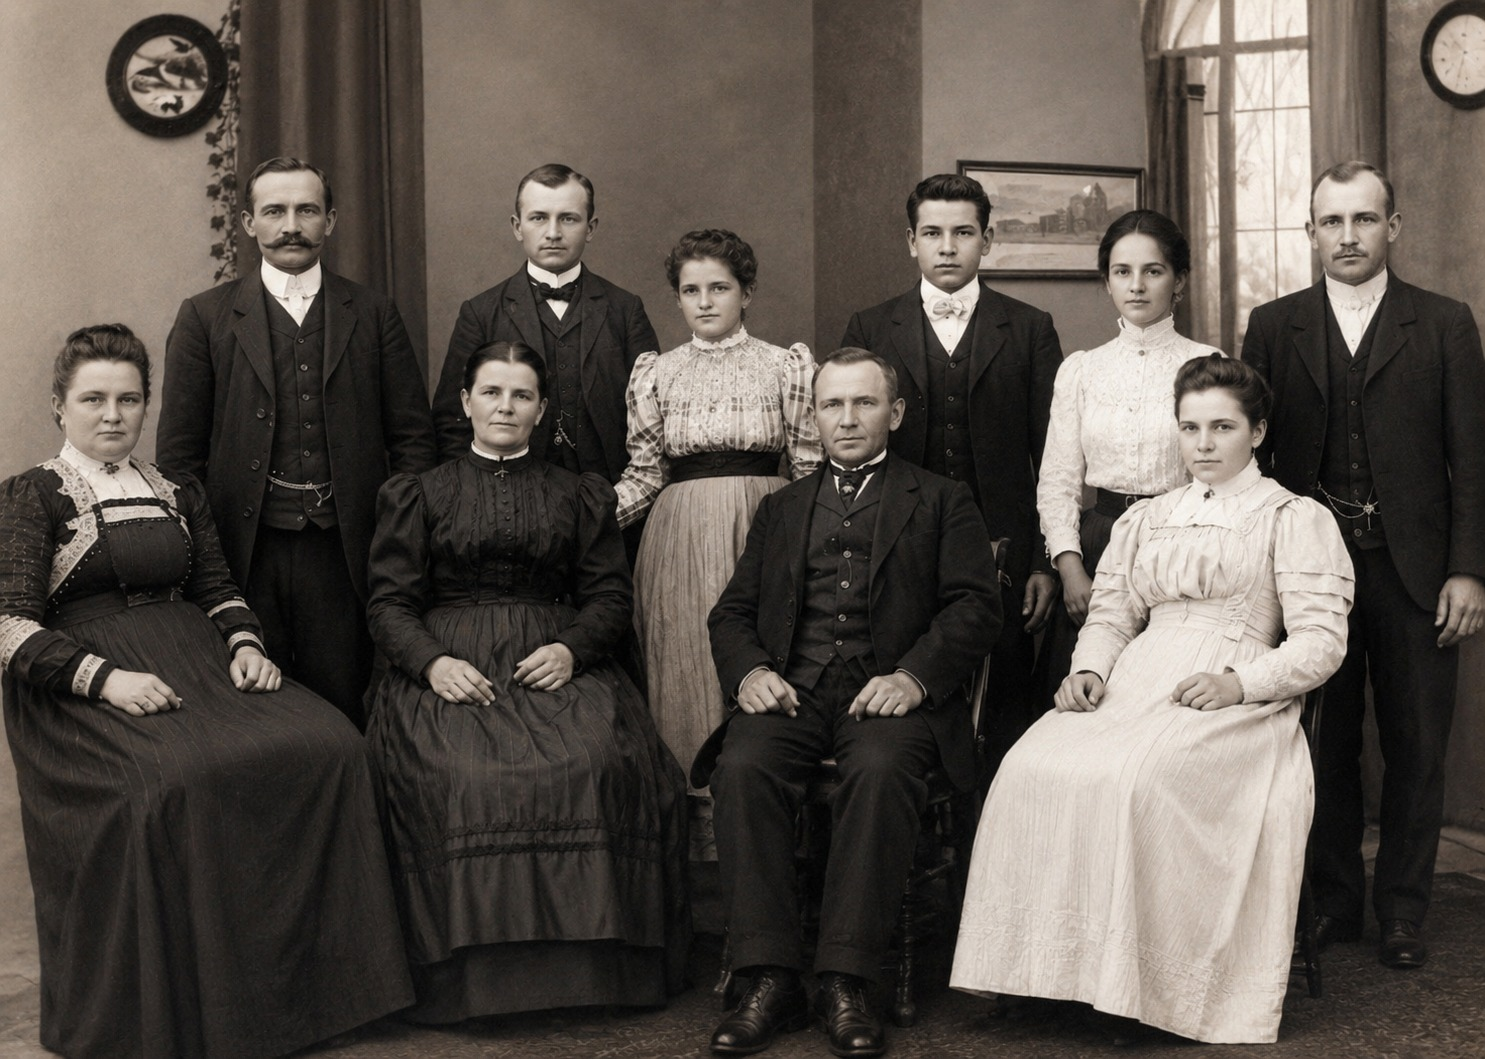
\includegraphics[width=0.85\linewidth,height=\textheight,keepaspectratio,alt={A família do Fata na Alemanha, antes de 1913. Acervo da família; a identificação individual de cada pessoa ainda está por confirmar. Versão restaurada com IA; o original está no repositório, e detalhes dos rostos podem ter sido retocados.}]{imagens/haas_familia_do_fata_alemanha_restaurada.jpg}
\caption{A família do Fata na Alemanha, antes de 1913. Acervo da
família; a identificação individual de cada pessoa ainda está por
confirmar. Versão restaurada com IA; o original está no repositório, e
detalhes dos rostos podem ter sido retocados.}
\end{figure}

Esta fotografia de estúdio chegou até nós com a legenda genérica de
``família do Fata na Alemanha''. Há onze pessoas: um casal mais velho
sentado ao centro, rodeado de moças de vestidos claros e rapazes de
colete e bigode. É tentador dizer que o casal sentado é Josef e
Franziska, e que um dos rapazes de pé é Johann. Eu mesmo, olhando para o
homem de bigode à esquerda, julguei reconhecer certa geometria do rosto.
Mas não sei. Não há nomes no verso que eu conheça. Prefiro deixar a
pergunta em aberto, como uma estação sem dados, a preencher o mapa com
um palpite que depois alguém vai citar como certeza.

O que a família guardou sobre Johann está no ofício. O texto do
centenário, escrito por minha irmã Marise Haas Lourenço em 2013, diz que
ele ``vinha de uma família de pedreiros e especializara-se em trabalhar
com gesso, emoldurando janelas, portais, altares''. Um estucador,
portanto: o artesão que, depois que o pedreiro levanta a parede, chega
para dar-lhe forma e ornamento. As cornijas das igrejas barrocas da
Baviera, os medalhões dos tetos, as molduras das janelas das casas
burguesas: tudo isso era trabalho de estucadores. Era um ofício de mãos
finas e paciência: preparar o gesso na consistência certa, correr o
molde de perfil ao longo da parede, modelar à mão as folhas, os anjos,
as volutas.

Johann vinha de uma cidade de fábrica, filho de operário. Ter chegado ao
gesso ornamental é, a meu ver, uma pequena ascensão social: do braço que
alimenta o forno à mão que desenha. Marise registrou outro detalhe que
me comove: ele era chamado com frequência para servir de intérprete,
porque dominava vários dialetos alemães, ``ainda muito presentes num
país cuja língua não estava unificada''. A Alemanha de 1900 era um país
recente, unificado politicamente havia apenas três décadas, e um bávaro
do Alto Palatinado podia ter dificuldade real para entender um saxão, um
suábio ou um homem do norte. Imagino Johann nas obras, entre equipes de
trabalhadores vindos de toda parte, traduzindo ordens do mestre de obras
para o dialeto de cada um. Um homem de ouvido bom, que trocava de
sotaque como quem troca de ferramenta.

Talvez por isso tenha sido, mais tarde, o contador de histórias que os
netos lembram. Quem passa a vida traduzindo aprende que toda frase tem
pelo menos duas versões.

\begin{figure}
\centering
\includegraphics[width=0.9\linewidth,height=\textheight,keepaspectratio,alt={De onde vieram: os lugares de origem dos ramos da família na Europa. Os pontos com interrogação vêm da tradição, não de documento. Mapa do autor.}]{imagens/mapa_europa_origens.jpg}
\caption{De onde vieram: os lugares de origem dos ramos da família na
Europa. Os pontos com interrogação vêm da tradição, não de documento.
Mapa do autor.}
\end{figure}

\section{Eibenstock, agosto de 1907}\label{eibenstock-agosto-de-1907}

Não sei como Johann e Maria se conheceram.

Essa é a frase que mais me custa escrever neste capítulo. Ele, de uma
vila siderúrgica perto de Regensburg; ela, de uma aldeia agrícola na
fronteira da Boêmia. Entre Sandberg e Heumaden há uns cinquenta
quilômetros em linha reta, longe o bastante para que dois jovens dessas
famílias dificilmente se cruzassem por acaso numa festa de igreja. E, no
entanto, se cruzaram. Se os avós de Johann vieram mesmo de Etzgersrieth,
como contei acima, a distância encolhe para quatro quilômetros, e o
acaso deixa de ser necessário.

O primo Agenor anotou que eles se casaram em 3 de agosto de 1907, em
Eibenstock. Se é a Eibenstock que eu conheço dos mapas, ela não fica na
Baviera, mas na Saxônia, nos Montes Metalíferos, perto da fronteira com
a Boêmia: uma região de mineração, de bordados e de reservatórios de
água, a uns cem quilômetros de Heumaden e bem mais de Sandberg. Ainda
não vi o registro desse casamento; não sei em que igreja foi, nem quem
foram as testemunhas. A Saxônia era majoritariamente luterana, e os dois
eram católicos. Tudo isso faz de Eibenstock uma das perguntas abertas
deste livro.

Tenho uma hipótese, que apresento como hipótese. O trabalho de Johann
era itinerante por natureza: o estucador vai aonde está a obra. E o de
Maria, segundo Marise, também a levava para fora de casa: ``Maria, além
dos trabalhos domésticos, recebia salário ordenhando vacas.'' Uma moça
de dezenove anos, filha de um pequeno lavrador com sete filhos, que
ordenhava vacas por salário, ou seja, nas propriedades dos outros. É o
retrato de uma filha que não ia herdar. O \emph{Anerbenrecht} de novo: a
terra dos Meier, em Heumaden, iria para um só dos irmãos, e os demais
teriam de buscar a vida onde houvesse trabalho. É perfeitamente possível
que os dois tenham se encontrado longe de casa, ambos trabalhando para
outros, num lugar que não era de nenhum deles. Mas é só isso, uma
possibilidade.

Há duas pistas que dão um endereço a essa possibilidade. A primeira é
uma lembrança da família: quando partiram para o Brasil, em 1913, Johann
e Maria moravam em Chemnitz, a grande cidade industrial da Saxônia, a
das fábricas de tecidos e de máquinas, que naqueles anos crescia
depressa e precisava de pedreiros. A segunda está numa gaveta da
família: cartas vindas da Alemanha com o endereço de remetente em
Dorfstadt, um bairro de Falkenstein, no Vogtland. Eibenstock fica entre
os dois, na beira dos Montes Metalíferos, a poucas dezenas de
quilômetros de Falkenstein e a pouco mais de Chemnitz. Se a lembrança
estiver certa, o casamento de 1907 deixa de ser um mistério de
geografia: não foi uma viagem até a Saxônia, foi um casamento na região
onde os dois já viviam e trabalhavam. E um porquê provável apareceu em
2026, nas cartas que conto no Capítulo 7: a família de Maria saiu de
Heumaden e foi parar no Vogtland, junto de Falkenstein, onde em 1971
ainda viviam três irmãs e um irmão dela. Se já estavam lá em 1907, Maria
casou perto da mãe. E continua a faltar o papel, que está no livro de
casamentos de Eibenstock e, se as crianças nasceram lá, nos registros de
Chemnitz.

O que Marise diz, e o que a família sempre repetiu, é que eles se
casaram jovens, ``com o sonho tão peculiar a todos nós de formar uma
família''. Johann tinha vinte e três anos; Maria, dezenove. Marise
acrescenta uma frase que eu acho certeira: era ela ``quem conhecia a
lida do campo e, certamente, o ponto de apoio para a grande jornada que
estavam próximos a empreender''.

\begin{figure}
\centering
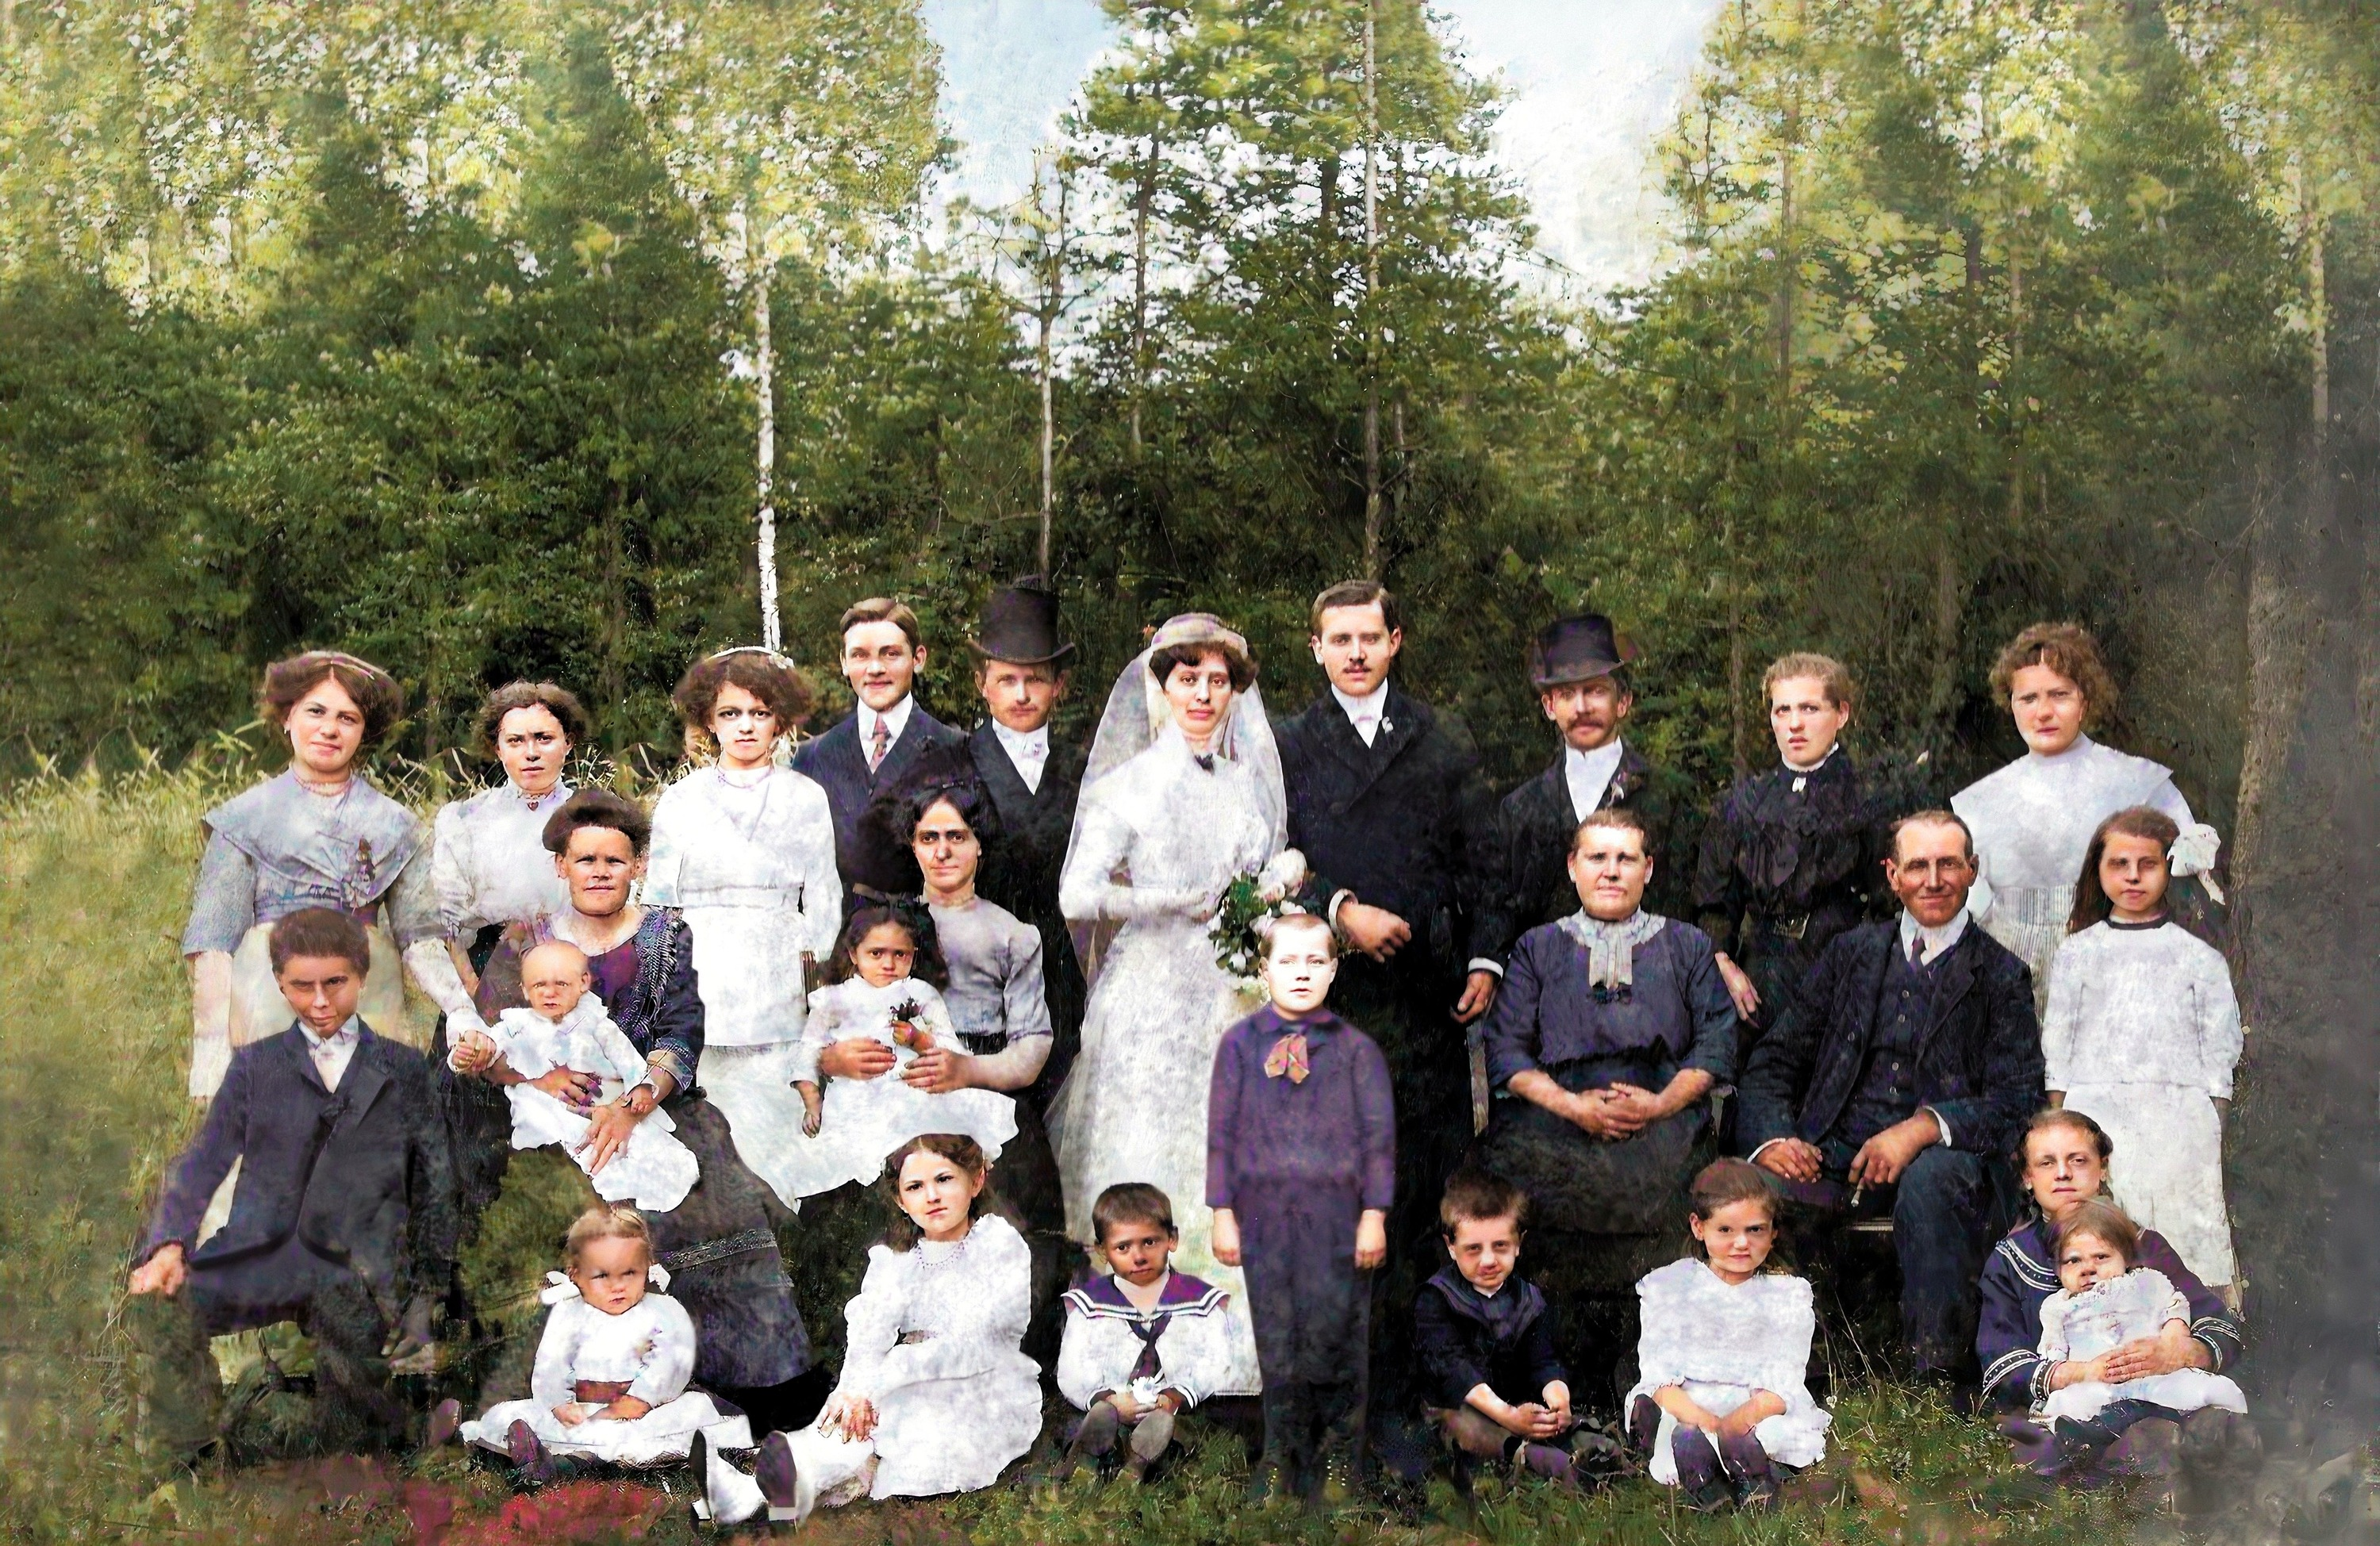
\includegraphics[width=0.85\linewidth,height=\textheight,keepaspectratio,alt={Fotografia de casamento da família da Mota na Alemanha, numa clareira de floresta. Acervo da família; o casal e os demais retratados ainda não foram identificados com segurança. Versão colorizada e restaurada com IA (MyHeritage); as cores são uma reconstrução, e o original em preto e branco está no repositório.}]{imagens/meier_familia_da_mota_alemanha_casamento_restaurada.jpg}
\caption{Fotografia de casamento da família da Mota na Alemanha, numa
clareira de floresta. Acervo da família; o casal e os demais retratados
ainda não foram identificados com segurança. Versão colorizada e
restaurada com IA (MyHeritage); as cores são uma reconstrução, e o
original em preto e branco está no repositório.}
\end{figure}

Esta outra fotografia sempre me intrigou. É um casamento, tirado ao ar
livre, numa clareira entre abetos e bétulas: a noiva de véu e buquê, o
noivo de bigode fino, dois homens de cartola, uma dúzia de crianças
sentadas na grama com roupas de domingo, senhoras de preto e moças de
branco. Chegou até mim como ``casamento da família da Mota''. Seria o
casamento de Johann e Maria? Seria o de um irmão ou irmã dela? Não sei.
A noiva não me parece ter dezenove anos, mas fotografias antigas
envelhecem as pessoas, e eu não confio no meu olho para isso. Coloco-a
aqui pelo que ela mostra com certeza: aquela gente, numa floresta muito
parecida com as de Heumaden, reunida para celebrar uma família que
começava.

Os primeiros anos do casamento, escreveu Marise, ``revelaram-se difíceis
e sofridos''. Aqui chegamos à parte do capítulo que eu gostaria de
pular.

Johann e Maria tiveram, na Alemanha, duas filhas que morreram pequenas:
Hildegard (o Agenor escreve Hildegart) e Frida. Não sabemos as datas de
nascimento, nem as de morte, nem a causa. ``Por razões que
desconhecemos'', diz o texto do centenário, com uma sobriedade que eu
respeito. Não sabemos onde estão sepultadas. Talvez em Eibenstock,
talvez em outro lugar onde o trabalho tenha levado o casal.

Em 1907, a mortalidade infantil na Alemanha ainda era alta; em muitas
regiões rurais e operárias, uma em cada cinco crianças não completava o
primeiro ano de vida. Dizer isso não diminui nada. Eu, que tenho dois
filhos, não consigo ler ``Hildegard e Frida'' sem parar um instante. São
os dois primeiros nomes de uma lista que este livro vai carregar até o
fim, a das crianças que não chegaram: cinco dos doze filhos do Fata e da
Mota. Os outros três nomes ainda não vou dizer. Vocês, Matheus e Lucas,
existem porque os outros sete aguentaram.

\section{Luisa, Walter e a decisão}\label{luisa-walter-e-a-decisuxe3o}

\emph{Alemanha, 1910 a 1913}

Em 1910 nasceu Luisa. Em 1912, Walter. Duas crianças vivas, depois de
duas perdas. Não sei onde nasceram; os registros que procuro ainda não
apareceram. Sei que estavam vivos e com saúde suficiente, em março de
1913, para atravessar a Europa de trem e embarcar num navio em Marselha,
e sei disso por um documento que vou mostrar no próximo capítulo, onde
os dois aparecem com as idades de dois anos e um ano.

No fim de 1912, Maria engravidou outra vez. Pelo menos é o que se
conclui do texto de Marise, porque o primo Agenor registrou as coisas de
outro modo.

Na planilha dele, há uma filha chamada Gertrudes nascida na Alemanha em
22 de outubro de 1911, que teria vindo no navio com um ano de idade. O
texto de Marise diz outra coisa: que Gertrudes nasceu no Brasil, em maio
de 1913, e que Maria embarcou grávida dela. Essas duas versões não podem
ser verdadeiras ao mesmo tempo, e no próximo capítulo vou colocá-las
lado a lado, com o documento que pesa mais. Por ora, sigo Marise: em
março de 1913, Johann e Maria tinham dois filhos pequenos e um terceiro
a caminho.

O que leva um casal assim a partir?

Marise fala da ``grande crise econômica e política'' da Alemanha e da
``iminência de uma guerra'' que ``assombrava o casal''. Gosto que ela
não tenha simplificado. A Alemanha de 1912 era, ao mesmo tempo, uma
potência industrial em plena expansão e um país de enormes
desigualdades, com o custo de vida subindo mais rápido que os salários
de operários e trabalhadores rurais. E o ar estava carregado. As crises
nos Bálcãs, a corrida naval com a Inglaterra, os orçamentos militares
crescendo ano a ano: tudo isso chegava às aldeias pelos jornais e pelas
conversas de taberna. Ninguém sabia exatamente o que ia acontecer, mas
muita gente pressentia que alguma coisa ia acontecer. Em meteorologia,
chamamos isso de instabilidade: a atmosfera acumula energia, a coluna de
ar fica pronta para subir, e falta apenas um gatilho.

Para um jovem pai de família, a guerra significava uma coisa muito
concreta: o alistamento. Johann tinha vinte e oito anos. É possível (e
aqui volto a especular) que o medo de ser convocado e deixar Maria
sozinha com os filhos tenha pesado tanto quanto a falta de dinheiro.

Do outro lado do oceano, havia o Brasil. Desde o fim do século XIX, o
governo brasileiro e os governos estaduais do Sul faziam propaganda na
Europa para atrair colonos: terra a preço baixo, pagável em prestações,
ferramentas, sementes, auxílio nos primeiros meses. Em Santa Catarina, o
governo federal havia aberto pouco antes um núcleo colonial no interior,
nas encostas da serra, com o nome de Anitápolis, em homenagem a Anita
Garibaldi, a heroína de Laguna. É para lá que os Haas iriam, ainda que
isso não estivesse claro no dia em que decidiram partir. Marise escreve
que eles iam ``para o paraíso'', com aspas que são dela, e que trazem
toda a ironia de quem sabe o que veio depois.

Eu suspeito que a terra, ela mesma, tenha sido o argumento decisivo. Um
pedreiro filho de operário e uma ordenhadeira filha de um pequeno
lavrador com sete filhos: nenhum dos dois ia herdar um pedaço de chão na
Baviera. Nem que vivessem cem anos. O \emph{Anerbenrecht} tinha fechado
essa porta antes mesmo que eles nascessem. No Brasil, diziam os
folhetos, havia lotes coloniais esperando por quem quisesse trabalhar.

Marise insiste num ponto que eu acho importante e que não quero apagar:
a decisão ``não foi arbitrária nem unilateral''. Os dois vinham de
famílias sólidas, nas quais ``o peso da opinião dos pais era tão grande
quanto o respeito que os filhos tinham por eles''. Houve conversas,
opiniões contra e a favor. Imagino a mesa da cozinha em Heumaden, numa
noite de inverno, com Georg Adam e Franziska ouvindo a filha dizer que
ia embora com o marido e os netos para um país do qual mal sabiam o nome
da capital. Imagino o silêncio depois.

\emph{Und wenn ihr nicht zurückkommt?} E se vocês não voltarem?

Não sei se alguém disse essa frase. Mas alguém deve ter pensado nela,
porque a fotografia que eles tiraram antes de partir tem a cara de uma
despedida definitiva. Marise escreveu que eles se despediram ``com
gestos que traduziam a certeza de que nunca mais se encontrariam''. Ela
estava certa: nunca mais se encontraram.

Quero terminar este capítulo com um exercício que faço com frequência no
trabalho. Quando analiso uma tempestade, procuro o momento em que ela se
tornou inevitável: o instante em que o ar quente e úmido encontrou a
frente fria e começou a subir, e a partir do qual nenhuma força pequena
poderia mais desfazê-la. Na genealogia dos Haas, esse instante não
aparece em nenhum documento. Ele aconteceu dentro de duas pessoas, numa
data que ninguém anotou, no inverno de 1912 para 1913. Antes dele, os
Haas eram bávaros com um futuro bávaro, provavelmente pobre,
provavelmente marcado pela guerra que viria. Depois dele, éramos nós.

No início de março de 1913, Johann, Maria, Luisa e Walter se puseram
diante de um fotógrafo, ao lado de parentes que ficariam. No dia 7, a
fotografia ganhou uma inscrição: \emph{Zum Andenken! vor unserer Abreise
nach Brasilien} (``Para recordação! Antes da nossa partida para o
Brasil''). Depois, imagino, vieram as malas, os livros que Marise diz
que eles levaram, as roupas de inverno que de nada serviriam do outro
lado, e uma estação de trem.

O trem ia para o sul. Para a França, para o mar.

\section{Para vocês descobrirem}\label{para-vocuxeas-descobrirem-3}

\begin{itemize}
\tightlist
\item
  Por que dois católicos da Baviera foram se casar em Eibenstock? O
  livro de casamentos de lá deve dizer em que igreja foi e quem foram as
  testemunhas.
\item
  Michael Haas e Kunigunde Stadelmann, os avós do Fata, eram mesmo de
  Etzgersrieth, vizinha de Heumaden? Procurem o batismo de Joseph Haas
  no livro de Moosbach, por volta de 1850.
\item
  Qual das duas listas de irmãos do Fata está certa, a do Agenor ou a
  dos livros de Leonberg?
\item
  Quem assinou as cartas de Dorfstadt, em Falkenstein, que estão numa
  gaveta da família?
\item
  Onde estão sepultadas Hildegard e Frida, e do que morreram? Se as duas
  nasceram em Chemnitz, comecem pelos registros de lá.
\item
  Quem são as onze pessoas da fotografia de estúdio da família do Fata?
  Mostrem a foto aos primos mais velhos: alguém sabe dizer um nome?
\end{itemize}

\chapter{Março de 1913: De Marselha ao Rio de Janeiro}\label{cap-5}

\emph{43,3° N · 5,4° L, Marselha · 22,9° S · 43,2° O, Rio de Janeiro}

\begin{quote}
\emph{Um rio não esquece o caminho até o mar. As famílias, às vezes,
esquecem; os papéis, quase nunca.}
\end{quote}

\section{\texorpdfstring{\emph{Zum
Andenken!}}{Zum Andenken!}}\label{zum-andenken}

Na fotografia de despedida há sete pessoas. Na lista do navio, quatro.

A fotografia mede pouco mais que a palma de uma mão, e a cópia que temos
é uma reprodução de reprodução, granulada, com as sombras empastadas.
Mesmo assim, é das imagens mais importantes deste livro. Na margem
esquerda, em letras brancas sobrepostas ao fundo escuro de arbustos,
alguém mandou imprimir: \emph{Zum Andenken! vor unserer Abreise nach
Brasilien, 7. März 1913.} ``Para recordação! Antes da nossa partida para
o Brasil, 7 de março de 1913.''

\begin{figure}
\centering
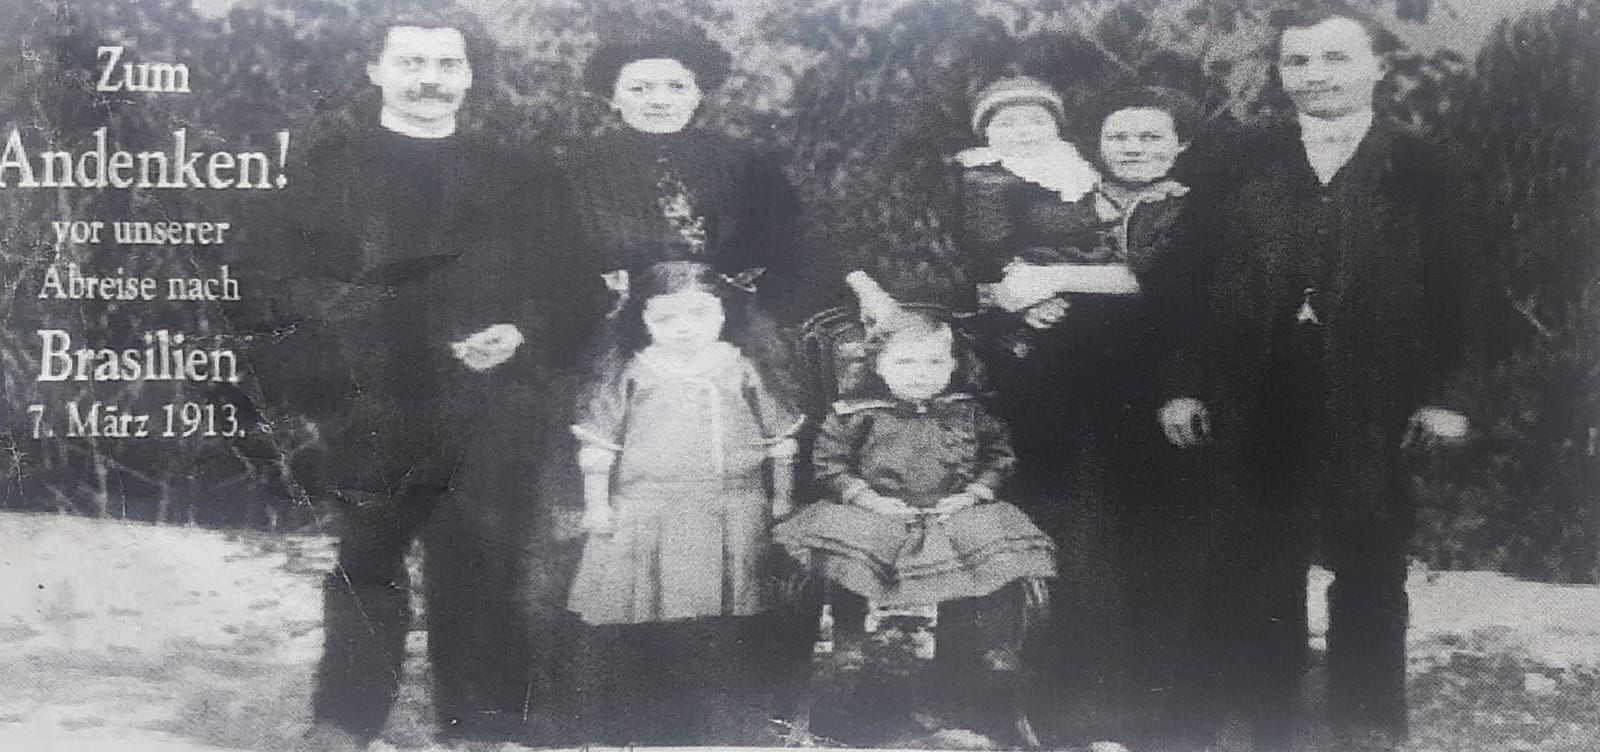
\includegraphics[width=0.9\linewidth,height=\textheight,keepaspectratio,alt={``Zum Andenken! vor unserer Abreise nach Brasilien, 7. März 1913.'' Fotografia de despedida tirada na Alemanha antes da viagem ao Brasil. Acervo da família; a identificação de cada pessoa retratada ainda não é segura.}]{imagens/haas_despedida_abreise_brasilien_1913.jpg}
\caption{\emph{``Zum Andenken! vor unserer Abreise nach Brasilien, 7.
März 1913.''} Fotografia de despedida tirada na Alemanha antes da viagem
ao Brasil. Acervo da família; a identificação de cada pessoa retratada
ainda não é segura.}
\end{figure}

Há sete pessoas na foto, de pé sobre um chão claro: terra batida, talvez
neve velha, é impossível dizer. À esquerda, um homem de bigode e roupa
escura, com as mãos juntas à frente do corpo. A seu lado, uma mulher de
cabelo preso no alto da cabeça, também de escuro. À direita, uma mulher
segurando no colo um bebê de touca e, ao lado dela, um homem jovem, sem
bigode, de paletó fechado. Entre os adultos, duas crianças: uma menina
de pé, de vestido claro e laço no cabelo, e uma criança menor sentada
numa cadeirinha de vime, com um vestido de babados.

Passei muito tempo olhando para essa imagem, e ela me deu mais perguntas
do que respostas. São quatro adultos e três crianças. Se Johann e Maria
estão ali (e a inscrição, na primeira pessoa do plural, ``nossa
partida'', sugere que sim), quem são os outros dois adultos? Um irmão,
uma irmã, um cunhado? E as três crianças: duas delas seriam Luisa, então
com uns dois anos, e Walter, com um? A menina de pé parece mais velha do
que dois anos. O bebê no colo parece mais novo do que um. Mas eu sei o
quanto as roupas de criança daquele tempo enganam (meninos de até três
ou quatro anos usavam vestido), e sei o quanto uma reprodução ruim
achata as proporções. Não vou forçar uma identificação. A família me
entregou essa foto como a despedida do Fata e da Mota, e é isso que ela
é. Quem é quem fica para os primos da Alemanha, se um dia os
encontrarmos, ou para outra cópia, mais nítida, que talvez esteja
guardada em alguma caixa.

O que a fotografia afirma sem ambiguidade é a data e a intenção. Em 7 de
março de 1913, alguém sabia que estava partindo para o Brasil e quis que
os que ficavam tivessem uma lembrança. A palavra \emph{Andenken} tem a
mesma raiz de \emph{denken}, pensar: é aquilo que faz pensar em alguém.
A foto foi feita para ser olhada por quem ficava. É uma ironia bonita
que ela tenha atravessado o oceano e chegado até nós, os que foram.

\section{Linhas 161 a 164}\label{linhas-161-a-164}

\emph{Marselha, março de 1913}

Os emigrantes alemães, em sua maioria, partiam de Hamburgo ou de Bremen,
os grandes portos do Mar do Norte. Os Haas partiram de Marselha. A
explicação que ouvi de meu pai é que, em 1913, o governo alemão,
prevendo a guerra, tinha proibido as emigrações, e por isso a família
saiu por um porto fora da Alemanha. Johann tinha 28 anos, idade de
servir. Ainda não achei a lei que confirme isso, e preciso saber se
houve uma proibição geral ou restrições aos homens em idade militar.
Outras razões podem ter pesado: uma passagem mais barata numa companhia
francesa, ou um agente de emigração que trabalhasse com os navios do
Mediterrâneo.

A história tem uma consequência para vocês. Por ter saído assim, a
família dava por impossível conseguir a cidadania alemã. Só que o Fata
nunca abriu mão da dele. Viveu no Brasil como estrangeiro e ia de tempos
em tempos à Polícia Federal se registrar. Se os papéis confirmarem isso,
a cidadania pode ter passado de pai para filho até vocês. Não sou
advogado: a resposta depende das leis alemãs da época e dos documentos,
e quem decide é a autoridade alemã. Mas é uma porta que pode estar
aberta, e foi o próprio Fata quem a deixou assim.

Imagino a viagem de trem: da Baviera para o sudoeste, atravessando a
fronteira francesa, descendo o vale do Ródano. Imagino o momento em que
o ar mudou. Quem sai do inverno continental bávaro e chega a Marselha no
início de março encontra outro mundo: luz mediterrânea, oliveiras, e
talvez o mistral, o vento frio e seco que desce pelo Ródano e varre o
porto em rajadas. Os bisavós trocaram o vento boêmio pelo mistral, e
logo trocariam o mistral pelos alísios. É assim que eu, por vício de
ofício, desenho a rota deles como uma sequência de ventos.

No porto, o vapor \emph{Formosa}. E, a bordo, uma lista.

\begin{figure}
\centering
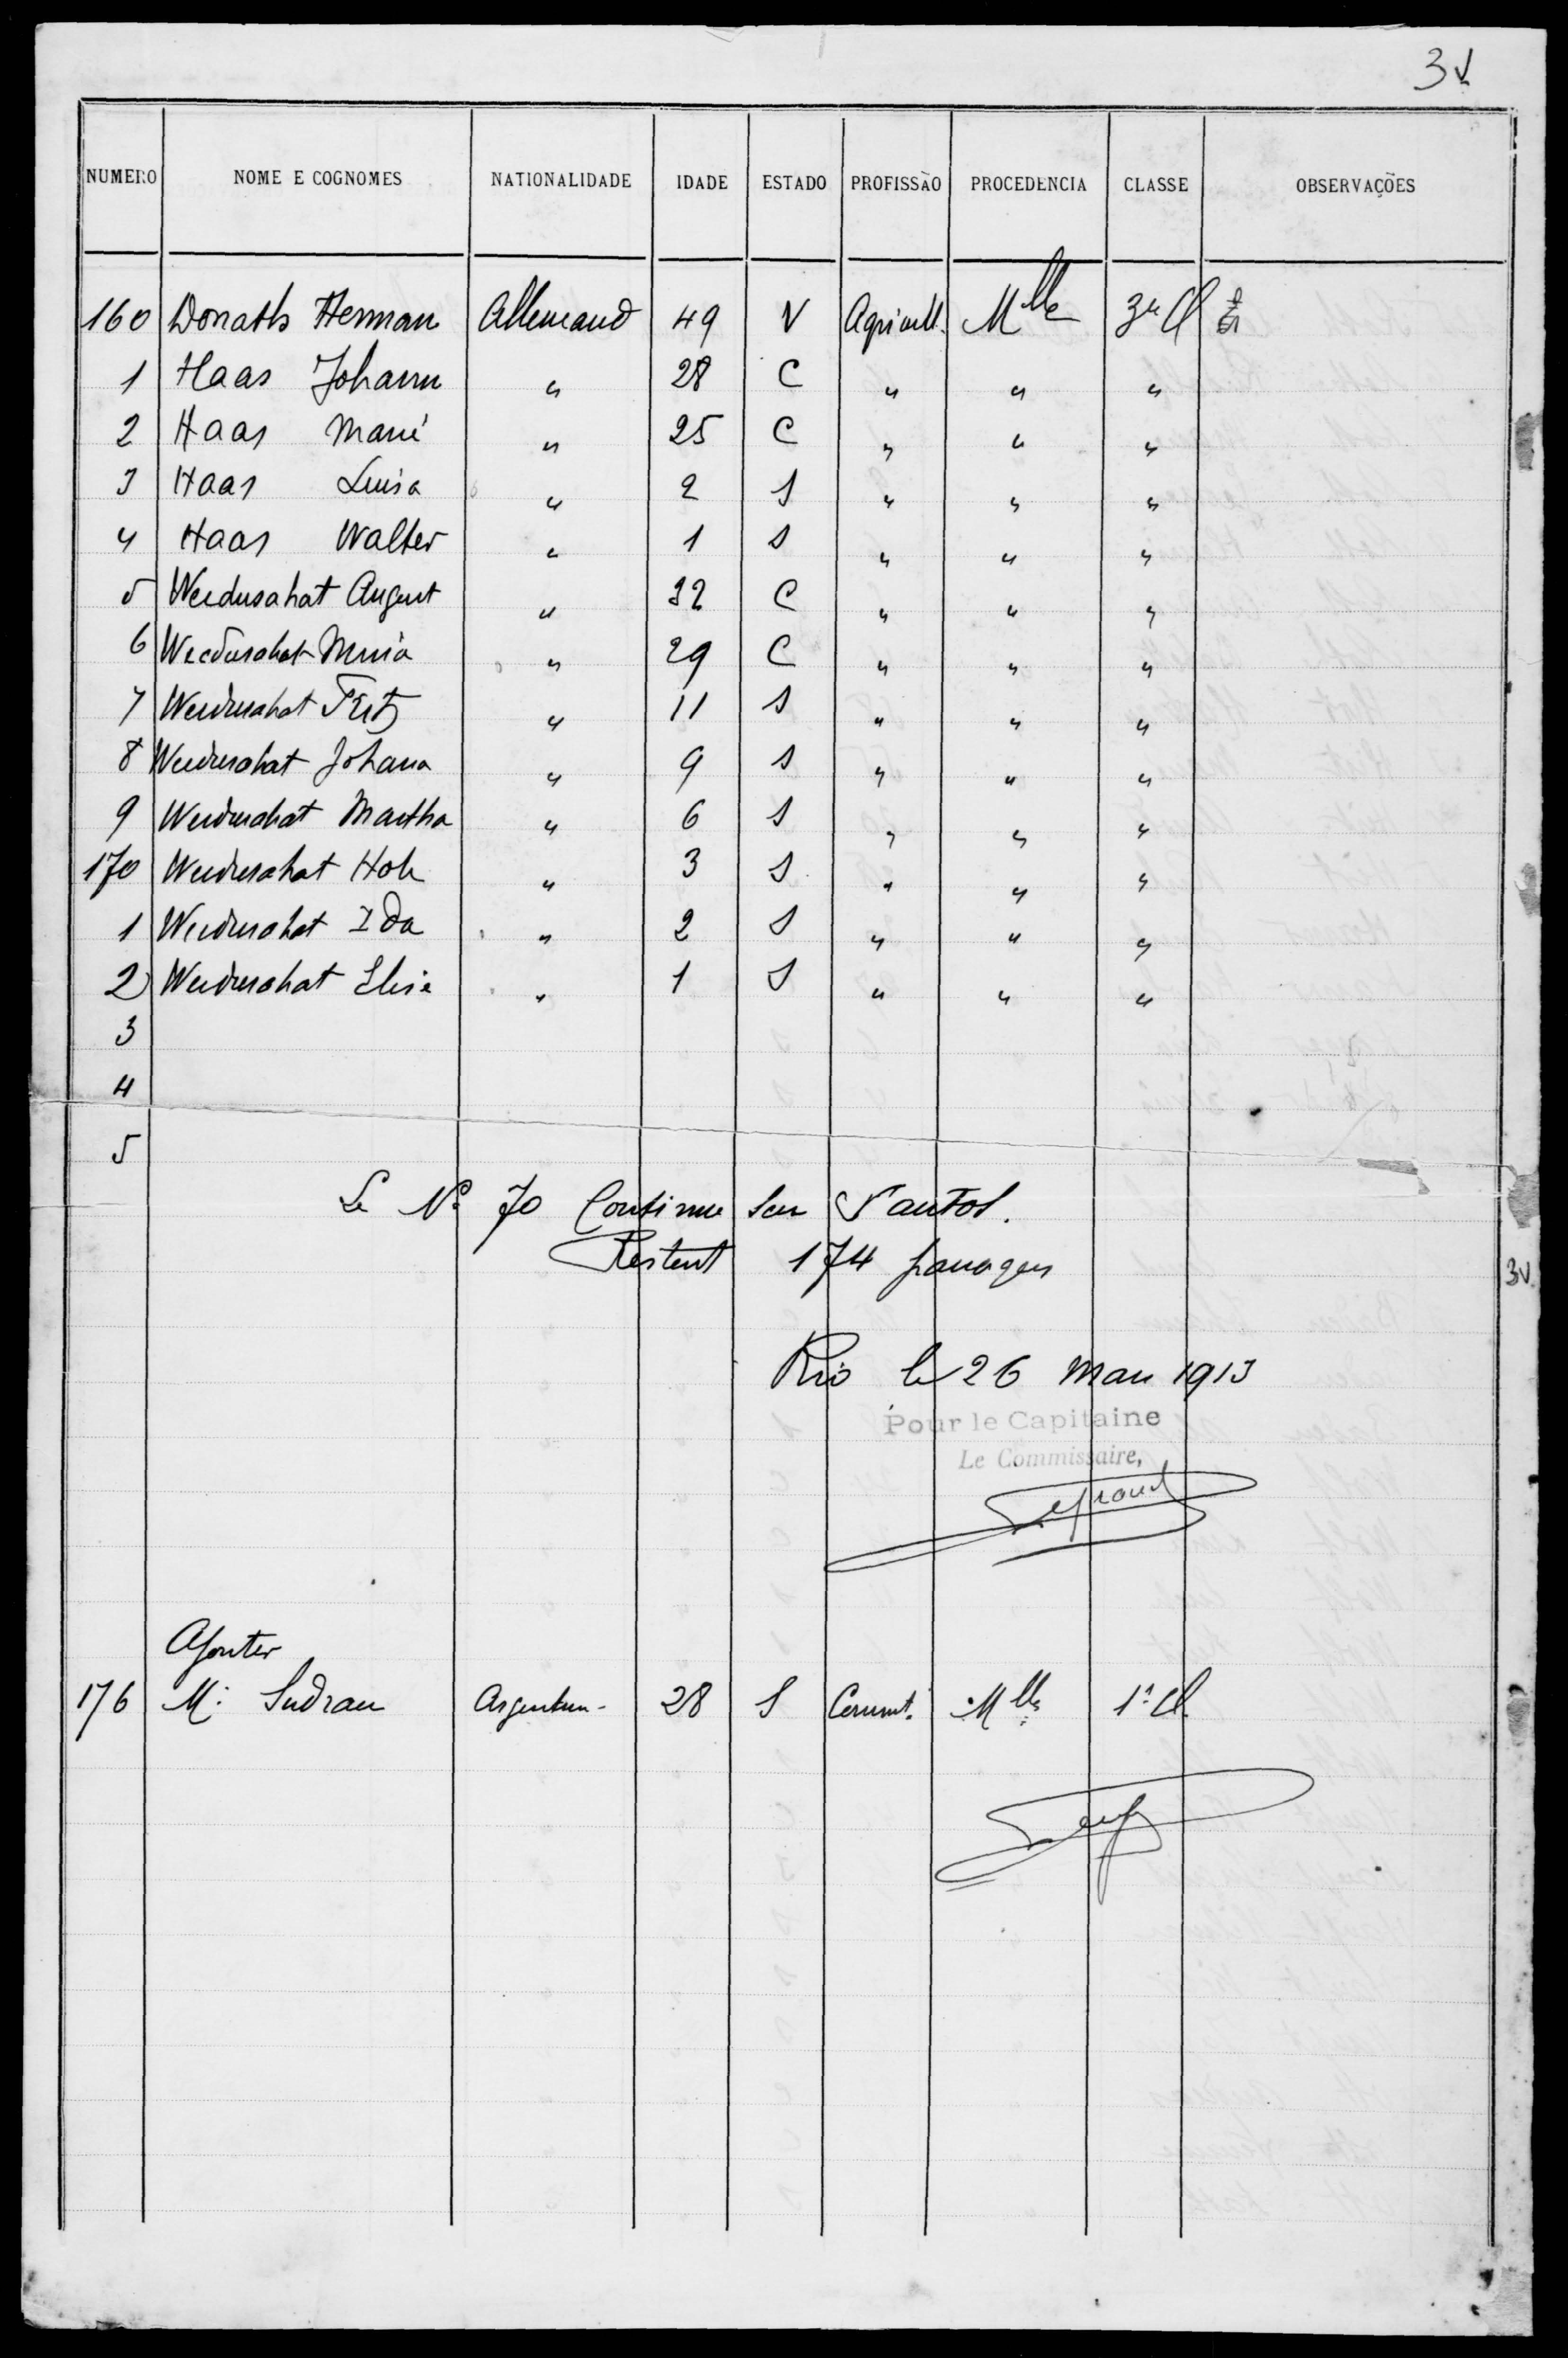
\includegraphics[width=0.9\linewidth,height=\textheight,keepaspectratio,alt={Manifesto de passageiros do vapor Formosa, folha 31, com a família Haas nas linhas 161 a 164: Johann, 28 anos; Marie, 25; Luisa, 2; Walter, 1. Ao pé, a nota ``Le Nº 70 continue sur Santos. Restent 174 passagers'' e a data ``Rio, le 26 Mars 1913''.}]{imagens/doc_haas_navio_formosa_1913.jpg}
\caption{Manifesto de passageiros do vapor \emph{Formosa}, folha 31, com
a família Haas nas linhas 161 a 164: Johann, 28 anos; Marie, 25; Luisa,
2; Walter, 1. Ao pé, a nota ``Le Nº 70 continue sur Santos. Restent 174
passagers'' e a data ``Rio, le 26 Mars 1913''.}
\end{figure}

\begin{ficha}

\textbf{Ficha do Arquivo}: Lista de passageiros do vapor \emph{Formosa},
procedente de Marselha, apresentada no Rio de Janeiro. Folha numerada
31. Colunas impressas em português (\emph{Numero, Nome e Cognomes,
Nationalidade, Idade, Estado, Profissão, Procedencia, Classe,
Observações}); preenchimento manuscrito em francês. Linhas 161 a 164:
\emph{Haas Johann}, 28, \emph{C} (casado); \emph{Haas Marie}, 25,
\emph{C}; \emph{Haas Luisa}, 2, \emph{S} (solteira); \emph{Haas Walter},
1, \emph{S}. Nacionalidade \emph{Allemand}, profissão \emph{Agricult.},
procedência \emph{M\textsuperscript{lle}} (Marselha) e
\emph{3\textsuperscript{e} Cl.} (terceira classe), todas indicadas por
aspas de repetição a partir da linha 160. Nota ao pé: \emph{``Le Nº 70
continue sur Santos. Restent 174 passagers.''} Data e assinatura:
\emph{``Rio, le 26 Mars 1913. Pour le Capitaine, Le Commissaire''}.
Imagem: \texttt{imagens/doc\_haas\_navio\_formosa\_1913.jpg}.

\end{ficha}

Quando vi esse documento pela primeira vez, a sensação foi parecida com
a de encontrar, numa série de dados que eu julgava perdida, uma
observação limpa, com hora e coordenada. Até então, tudo o que tínhamos
da viagem de 1913 era memória oral, recontada muitas vezes. De repente,
havia um papel escrito por alguém de fora da família, no próprio ano,
que dizia: eles estavam aqui.

O papel diz coisas que a memória não dizia. Diz que Johann se declarou
\emph{agriculteur}, agricultor, e não estucador, o que faz todo o
sentido, porque o Brasil queria colonos para a lavoura, não artesãos de
cidade, e é provável que o agente de emigração tenha orientado todos a
se declararem assim. Diz que Maria tinha vinte e cinco anos, quando na
verdade, em março de 1913, ainda tinha vinte e quatro: só completaria
vinte e cinco em 7 de abril, já do lado de cá do oceano. Uma diferença
pequena, do tipo que se arredonda num guichê. Diz que eles viajaram de
terceira classe, como quase todos os emigrantes. E diz, sem nenhuma
ambiguidade, que a bordo estavam Luisa, de dois anos, e Walter, de um.

Mais abaixo, na mesma folha, vem uma família inteira de sobrenome
difícil de ler (algo como \emph{Weidushat}), com pai, mãe e seis filhos
de onze anos para baixo. Fico pensando nas conversas na terceira classe
entre Maria e aquela outra mãe, com seis crianças. Não sei nada sobre
eles. Sei que dividiram a mesma página, e provavelmente o mesmo porão.

Não sei também como foi a travessia. Dezessete ou dezoito dias, talvez,
de Marselha ao Rio: o Mediterrâneo, o estreito de Gibraltar, a costa
africana, a calmaria equatorial, os alísios de sudeste. Para uma mulher
talvez grávida, cuidando de um bebê de um ano e de uma menina de dois,
num porão de terceira classe, imagino que cada um desses dias tenha sido
longo. Não vou inventar tempestades. A reanálise de 1913 é grosseira
demais para me dizer o que o \emph{Formosa} enfrentou, e eu prefiro o
silêncio honesto ao drama inventado.

Sei que chegaram ao Rio em 26 de março. O manifesto diz.

\begin{figure}
\centering
\includegraphics[width=0.85\linewidth,height=\textheight,keepaspectratio,alt={A viagem de 1913, de Marselha ao Rio de Janeiro. O traçado é esquemático: não conheço a rota nem as escalas desta viagem, e o ponto de entrada em Santa Catarina continua em aberto. Mapa do autor.}]{imagens/mapa_viagem_1913.jpg}
\caption{A viagem de 1913, de Marselha ao Rio de Janeiro. O traçado é
esquemático: não conheço a rota nem as escalas desta viagem, e o ponto
de entrada em Santa Catarina continua em aberto. Mapa do autor.}
\end{figure}

\section{O que o papel diz, e o que ele não
diz}\label{o-que-o-papel-diz-e-o-que-ele-nuxe3o-diz}

\emph{Rio de Janeiro, 26 de março de 1913}

Durante muitos anos, a família contou a chegada de um jeito só. O texto
do centenário, escrito por Marise em 2013, registrou essa versão: o
desembarque no Rio teria sido recusado, o navio teria seguido de porto
em porto pela costa cumprindo quarentena, com gente demais, comida ruim
e ``inúmeros óbitos'' a bordo, até que a família desceu, exausta, em
Laguna.

Preciso ser claro com vocês, porque as primeiras versões deste livro se
apoiaram demais nesse texto. Ele foi escrito cem anos depois dos fatos,
a partir de lembranças de terceira e quarta mão, para ser lido numa
festa. Tem o mérito enorme de ter juntado o que a família sabia. Mas,
onde pode ser comparado com documentos, erra com frequência. Por isso a
regra deste livro é simples: \textbf{quando o papel da época e a
tradição discordarem, fico com o papel}, e a tradição passa a ser uma
pergunta, não uma resposta.

O papel da época, neste ponto, é a lista do \emph{Formosa}. Foi assinada
no Rio de Janeiro, em 26 de março de 1913, pelo comissário de bordo,
para ser entregue às autoridades brasileiras. Nela estão vivos, nas
linhas 161 a 164, os quatro Haas: Johann, Marie, Luisa e Walter. Ninguém
da família morreu na travessia. A coluna de observações, onde se
anotaria um óbito a bordo, está vazia. A nota do pé da página
(\emph{``Le Nº 70 continue sur Santos. Restent 174 passagers''}) diz que
um passageiro seguia para Santos e que os demais ficavam. O Rio era o
porto de chegada da família. Nenhum documento que eu tenha visto fala em
desembarque recusado, em navio vagando pela costa ou em mortes a bordo.

O que o papel não diz é o que veio depois. Os recém-chegados passavam,
em geral, pela Hospedaria de Imigrantes da Ilha das Flores, na baía de
Guanabara, e dali eram encaminhados aos estados de destino. Os registros
da Ilha das Flores e da Inspetoria de Imigração, guardados no Arquivo
Nacional, devem dizer quando os Haas saíram do Rio, em que navio e para
que porto de Santa Catarina. Pode ter sido Florianópolis, onde o primo
Agenor procurou sem achar, ou Laguna, como diz a tradição. Enquanto
esses livros não forem abertos, não sei. E não vou preencher o intervalo
com quarentenas e tempestades.

\section{Gertrudes}\label{gertrudes}

O mesmo vale para o nascimento de Gertrudes. A tradição diz que ela
nasceu em 5 de maio de 1913, no Barracão dos Imigrantes de Laguna. A
planilha do primo Agenor diz que nasceu na Alemanha, em 22 de outubro de
1911, e veio no navio. O manifesto não traz nenhuma Gertrudes a bordo, e
isso já tornava a data de 1911 difícil de sustentar: uma menina de
dezesseis meses estaria na lista, como estão as crianças de um ano da
mesma página.

O papel que faltava apareceu nos índices de registros católicos de Santa
Catarina. Gertrud, filha de Johann Haas e Maria Meyer, foi batizada em
23 de novembro de 1913 na paróquia de Teresópolis, hoje Águas Mornas,
que atendia o núcleo colonial de Anitápolis. O perfil dela no
FamilySearch dá o nascimento em 5 de maio de 1913, em Anitápolis. A data
da tradição estava certa; o lugar, provavelmente não. Gertrudes nasceu
cerca de seis semanas depois da chegada ao Rio, e Maria, portanto,
viajou grávida, como a família sempre contou. Gertrudes cresceu, casou
em maio de 1932 em Ituporanga com Augusto Sebold, filho de colonos de
Teresópolis, e foi com ele para o norte do Paraná. Morreu em 23 de junho
de 1997, em Pindauvinha, no município de Ivaiporã.

\begin{ficha}

\textbf{Ficha do Arquivo}: Batismo de Gertrud Haas, filha de Johann Haas
e Maria Meyer, em 23/11/1913, paróquia de Teresópolis (SC): ``Brasil,
Santa Catarina, Registros da Igreja Católica, 1714--1977'',
FamilySearch, ark:/61903/1:1:QPQC-X62B. Casamento com Augusto Sebold:
religioso em 07/05/1932 e civil em 09/05/1932, Ituporanga (``Brasil,
Santa Catarina, Registro Civil, 1850--1999'', ark:/61903/1:1:X9B4-G1T4).
A data de nascimento (05/05/1913, Anitápolis) e a de óbito (23/06/1997,
Pindauvinha, Ivaiporã, PR) vêm do perfil G8P8-X9D, ainda sem certidão
anexada.

\end{ficha}

\section{Onde estão Luisa e Walter}\label{onde-estuxe3o-luisa-e-walter}

Sobre as duas crianças do \emph{Formosa}, a tradição escrita também se
enganou. O texto do centenário diz que Luisa e Walter morreram ainda nos
barracões, enfraquecidos pela viagem. A planilha de Agenor, porém,
registra duas crianças, ``Lina'' e ``Valter'', sepultadas em Rio do
Ouro, Anitápolis, o lugar para onde a família foi depois da chegada. E
há uma testemunha que eu ouvi com meus próprios ouvidos: meu pai.

Baldoíno me contou que foi com os irmãos a Anitápolis buscar os restos
dos irmãos pequenos, para trazê-los a Ituporanga. Foi nessa viagem, na
serra, que ele viu neve pela primeira vez. Walter está hoje sepultado em
Ituporanga, junto da família. As crianças, portanto, sobreviveram à
viagem, chegaram a Rio do Ouro e morreram lá. Anos depois, os irmãos
foram buscá-las.

``Lina'' é, muito provavelmente, a Luisa da lista de bordo, com o nome
de casa; ``Valter'' é o Walter escrito à brasileira. Ainda não sei as
datas das mortes, nem o ano do traslado, nem em que inverno nevou na
serra para meu pai ver. Mas a história agora se apoia em três pernas: um
documento de bordo, uma planilha montada com cuidado e o relato de quem
carregou os restos. Já não depende de uma frase escrita para uma festa.

O resto continua em aberto. A data de partida que Agenor anotou, 13 de
março, não combina com a fotografia de 7 de março nem com a chegada ao
Rio no dia 26. A fotografia pode marcar a despedida em casa, e não o
embarque em Marselha; a viagem de trem até a França levava dias. O dia
26 de abril, também anotado por ele, cai exatamente um mês depois da
chegada ao Rio: pode ser a chegada a Santa Catarina, depois da
hospedaria e do navio costeiro, ou um simples erro de mês. O batismo de
Gertrudes em Teresópolis sugere que a família subiu para Anitápolis pelo
caminho de Florianópolis, Palhoça e Teresópolis, e não por Laguna; mas a
lista do navio costeiro ainda não foi encontrada. Essas perguntas estão
listadas, uma a uma, no fim deste livro, para quem quiser procurar.

\section{Laguna, fevereiro de 2012}\label{laguna-fevereiro-de-2012}

Em fevereiro de 2012, fomos a Laguna e a Tubarão: eu, Bárbara, Matheus e
Lucas. Matheus tinha nove anos; Lucas ia fazer sete. Não eram muito mais
velhos do que Luisa e Walter quando atravessaram o oceano.

Na época, eu ainda não tinha o manifesto do \emph{Formosa} nem sabia de
todas essas contradições. Sabia o que a família repetia: que o Fata e a
Mota tinham chegado por Laguna e que ali estavam as primeiras covas da
família no Brasil. Hoje sei que a segunda parte está errada, porque as
covas estavam em Anitápolis, e que a primeira ainda espera documento.
Mas fomos olhar a cidade com essa ideia na cabeça.

Laguna é uma das cidades mais antigas de Santa Catarina, fundada no
século XVII. O centro histórico tem casario colonial português, a igreja
matriz de Santo Antônio dos Anjos, ruas estreitas que descem para a
lagoa. Foi a terra de Anita Garibaldi e o palco da efêmera República
Juliana de 1839. É também a cidade dos botos que, há gerações, conduzem
os cardumes de tainha na direção das tarrafas dos pescadores na barra,
uma cooperação entre espécies que os biólogos estudam até hoje. É,
sobretudo, uma cidade construída em torno de uma passagem de água: a
barra que liga o sistema de lagoas ao oceano, por onde entravam e saíam
os navios.

Se os bisavós entraram por ali, não deixaram marca. Não há placa, não há
registro no cais, não há memorial do Barracão dos Imigrantes que eu
tenha encontrado. Há só a barra e a água entrando e saindo com a maré.

Em Tubarão, a poucas dezenas de quilômetros rio acima, vimos o acervo de
Willy Zumblick, o pintor da cidade, que dedicou boa parte da vida a
retratar a história do sul catarinense: Anita, Garibaldi, os lanchões da
República Juliana, a paisagem do litoral. Eu gosto de pintores
históricos pela mesma razão que gosto de reanálises: eles reconstroem o
que ninguém fotografou, sabendo que estão reconstruindo.

Deixo o resto daquela viagem com os meninos e com a Bárbara, que guardam
dela as lembranças deles. A minha, a que importa para este livro, é uma
imagem de geógrafo: Laguna fica na foz de um rio. O rio é o Tubarão.

\section{O rio que desce para a
barra}\label{o-rio-que-desce-para-a-barra}

Quem chega a Laguna pelo mar não vê o rio Tubarão. Ele desemboca no
complexo de lagoas por trás da cidade, depois de descer da Serra Geral,
atravessar a cidade de Tubarão e serpentear pela planície costeira. A
água que sai pela barra de Laguna é, em boa parte, água que choveu na
serra.

Em março de 1974, essa água desceu toda de uma vez.

Nos dias 24 e 25 de março de 1974, uma enchente devastou a cidade de
Tubarão. Foi o maior desastre natural da história de Santa Catarina até
então. Os números oficiais mais citados falam em cerca de duzentos
mortos e dezenas de milhares de desabrigados. Bairros inteiros ficaram
submersos; a cidade levou anos para se refazer. Depois da tragédia, o
rio foi retificado e canalizado no trecho urbano: as curvas que a água
tinha desenhado durante milênios foram cortadas por engenheiros que, com
razão, não queriam ver aquilo de novo.

Eu tinha oito anos em março de 1974. Ainda não pensava em ser
meteorologista. Hoje, quando olho para aquele evento, vejo o que a minha
profissão me ensinou a ver: uma bacia hidrográfica que nasce em escarpas
íngremes, recebe chuva orográfica quando o ar úmido do oceano é
empurrado contra a serra, concentra essa água em poucas horas e a
despeja numa planície baixa, onde ela não tem para onde ir a não ser
para os lados. Em 1973 e 1974, o Pacífico estava em fase de La Niña.
Muita gente gosta de procurar no El Niño e na La Niña a explicação de
cada desastre, e eu preciso ser cuidadoso aqui: essas oscilações mudam
as probabilidades, não decidem o destino. O clima carrega os dados; quem
joga é o tempo, dia após dia. Uma frente que estaciona, um sistema que
se aprofunda, um fluxo de leste que persiste por mais um dia: é isso que
transforma uma estação chuvosa numa catástrofe.

Trabalho há anos com modelagem de cheias, hidrologia e previsão. Passei
boa parte da carreira tentando antecipar o que os rios de Santa Catarina
vão fazer quando a chuva vier: o Itajaí, o Tubarão, e também o Taquari,
lá no Rio Grande do Sul, de onde vem a família de Bárbara. Não vou
detalhar projetos aqui. Quero registrar uma coincidência que só percebi
ao escrever este capítulo: a cidade que a família sempre apontou como a
sua porta de entrada fica na boca de um rio que, seis décadas depois,
faria a maior tragédia da história do estado. E o neto deles, sem saber
dessa ligação, escolheria passar a vida estudando exatamente esse tipo
de água.

Este livro vai voltar às enchentes. No capítulo 13, os três rios das
nossas famílias (o Tubarão, o Itajaí e o Taquari) aparecem juntos,
porque a chuva que cai sobre eles é, muitas vezes, uma só. Por ora,
deixo apenas esta imagem: a barra de Laguna como uma porta de entrada.
Por ela entraram navios de imigrantes; por ela sai, todo dia, a chuva da
serra. Se os Haas passaram por ela, foi uma vez, de fora para dentro. O
rio passa por ela sempre, de dentro para fora.

Em algum dia de 1913 que nenhum papel encontrado até agora registra,
Johann e Maria chegaram ao litoral catarinense e subiram a serra.
Levavam Luisa e Walter, ainda vivos, e, cedo ou tarde, uma recém-nascida
chamada Gertrudes. À frente, as encostas da serra e a promessa de um
lote de terra num lugar chamado Rio do Ouro.

O nome, como tantos outros nomes daquela época, era uma promessa que a
terra não ia cumprir.

\section{Para vocês descobrirem}\label{para-vocuxeas-descobrirem-4}

\begin{itemize}
\tightlist
\item
  A Alemanha proibiu mesmo a emigração em 1913, como meu pai contava?
  Por que os Haas embarcaram em Marselha, se a maioria dos emigrantes
  alemães partia de Hamburgo ou de Bremen?
\item
  Onde estão as fichas de estrangeiro do Fata, dos registros que ele
  fazia na Polícia Federal? Elas podem ser a prova de que ele continuou
  alemão.
\item
  Em que navio e por que porto a família chegou a Santa Catarina:
  Laguna, Florianópolis ou outro? Os livros da Ilha das Flores e da
  Inspetoria de Imigração, no Arquivo Nacional, devem dizer.
\item
  Quem são os outros dois adultos da fotografia de 7 de março, e de quem
  são as três crianças? Perguntem aos primos se existe, em alguma caixa,
  uma cópia mais nítida.
\item
  Em que inverno nevou na serra, na viagem em que Baldoíno e os irmãos
  foram buscar os restos das crianças? Perguntem aos primos mais velhos
  se ouviram essa história dos pais deles.
\end{itemize}

\chapter{Os Anjos de Gesso de Rio do Ouro e as Clareiras de
Ituporanga}\label{cap-6}

\emph{27,9° S · 49,1° O, Rio do Ouro, Anitápolis · 27,4° S · 49,6° O,
Ituporanga, SC}

\begin{quote}
\emph{O gesso endurece em minutos. A terra, em gerações. Quem trabalha
com os dois aprende a esperar de jeitos diferentes.}
\end{quote}

\section{Uma carta de Heumaden}\label{uma-carta-de-heumaden}

\emph{Rio do Ouro, Santa Catarina, fim de 1914}

Em algum momento entre o fim de 1914 e o início de 1915 (não sei a data,
e a carta, se ainda existir, nunca passou pelas minhas mãos), chegou ao
interior de Santa Catarina uma carta da Alemanha. Vinha de uma irmã da
Mota. Podia ser Barbara, a mais velha das meninas, ou Margaretha, ou a
pequena Anna, que em 1914 teria uns dezesseis anos. O que a família
lembra é o conteúdo: a guerra tinha começado. Não tentassem voltar.

Marise, no texto do centenário, conta isso de passagem, numa frase que
esconde muito: ``mesmo desesperados, infelizes e querendo fazer o tempo
voltar, não poderiam mais retornar à Alemanha, pois uma carta recebida
de uma irmã da Mutter alertava-os para o início da Guerra''.
\emph{Mutter}, mãe: a palavra que os netos brasileiros, de ouvido,
transformaram em Mota.

Eu fico pensando no que essa frase revela. Revela, primeiro, que eles
queriam voltar. Pouco mais de um ano depois de chegar, com dois filhos
enterrados e uma terra que não produzia, Johann e Maria consideravam
seriamente o caminho de volta. E revela que alguém, em Heumaden, sabia
disso: que eles escreviam para casa, contavam o que estava acontecendo,
e que a família da Baviera respondia. Havia um fio, ainda. A carta da
irmã foi, ao mesmo tempo, a notícia que cortou esse fio e uma prova de
que ele existia.

Imagino Maria lendo a carta em voz alta para Johann à luz de um lampião,
numa casa de madeira no meio da encosta. Imagino o silêncio de duas
pessoas que acabam de entender que a porta atrás delas se fechou. Daqui
por diante, o único caminho era para a frente, e, como diz Marise, ``não
estavam sós, tinham Gertrudes e muitos companheiros na mesma situação''.

\begin{figure}
\centering
\includegraphics[width=0.9\linewidth,height=\textheight,keepaspectratio,alt={Santa Catarina da família: os rios e os lugares por onde os ramos Haas, Dörner, Preis, Michels e Arns passaram. Os rios vêm do meu modelo de cheias. Mapa do autor.}]{imagens/mapa_santa_catarina.jpg}
\caption{Santa Catarina da família: os rios e os lugares por onde os
ramos Haas, Dörner, Preis, Michels e Arns passaram. Os rios vêm do meu
modelo de cheias. Mapa do autor.}
\end{figure}

\section{O Lote 17}\label{o-lote-17}

\emph{Rio do Ouro, Núcleo Colonial de Anitápolis, 1913 a 1918}

Do litoral, por um porto que ainda não sei qual foi, a família foi para
o interior, subindo as encostas da Serra Geral até um lugar chamado Rio
do Ouro. Hoje, Rio do Ouro pertence ao município de Anitápolis, na
região serrana a sudoeste da Grande Florianópolis. Naquele tempo,
pertencia a Palhoça; é assim que o primo Agenor registra o nascimento de
Alexandre, o pai dele: ``em Rio do Ouro, Palhoça, hoje pertence a
Anitápolis''.

\begin{ficha}

\textbf{Ficha do Arquivo}: Planilha genealógica de Agenor Haas, nota
biográfica sobre Alexandre Haas: \emph{``nasceu no dia 23 de maio de
1917, em Rio do Ouro, Palhoça, hoje pertence a Anitápolis, SC, era
pedreiro''}. Na nota sobre os patriarcas, Agenor anota que Johann
\emph{``viveu até 1918 na localidade Rio do Ouro, em Anitápolis, SC,
quando mudou-se para Rio Novo em Ituporanga''}. Fonte: transcrição da
planilha original \texttt{.xls}, guardada no arquivo privado da família.

\end{ficha}

Anitápolis era um núcleo colonial aberto pelo governo federal poucos
anos antes, nas cabeceiras de rios que descem da serra, para receber
imigrantes europeus. O nome homenageava Anita Garibaldi, a heroína de
Laguna. Essa volta me agrada: se a tradição estiver certa, a família
entrou em Santa Catarina pela terra de Anita e foi viver no lugar
batizado com o nome dela. Mais tarde, a partir de 1918, as instalações
do núcleo abrigariam um Patronato Agrícola, uma escola-internato para
meninos pobres e órfãos que o governo queria transformar em
trabalhadores do campo.\footnote{Sobre o Patronato Agrícola de
  Anitápolis (1918--1930), ver Daniel Alves Boeira, \emph{Uma
  ``solução'' para a menoridade na Primeira República: o caso do
  Patronato Agrícola de Anitápolis/SC (1918--1930)}, dissertação de
  mestrado, UDESC, 2012, citada por Juliana da Silva Monteiro e Maria do
  Carmo Brazil na \emph{Revista HISTEDBR On-line}, v. 19, 2019.} Mas
isso já seria depois da partida dos Haas.

Marise conta que ``junto com um amigo, compraram um pedaço de terra. O
Lote 17, em Rio do Ouro''. Não sei quem era o amigo: outro imigrante do
barracão, talvez, alguém da mesma viagem. A compra em sociedade diz
muito sobre o quanto eles tinham: nem o suficiente para um lote inteiro.
E o lote, escreve Marise, era ``uma terra ingrata: seca e ácida, sem
capacidade de boa produção de alimentos nem para a própria subsistência.
Até descobrirem quão inférteis eram, já haviam investido o pouco que
tinham.''

Quero me deter nessa frase porque ela diz alguma coisa sobre a ciência
do solo e sobre a política de colonização. Os solos das encostas da
Serra Geral catarinense, formados a partir de rochas antigas e lavados
por chuvas abundantes durante milênios, tendem a ser ácidos e pobres em
nutrientes. Debaixo da mata atlântica, enganam: a floresta parece
exuberante porque recicla os próprios nutrientes, as folhas que caem
alimentam as raízes que sobem. Derrubada a mata e queimada a coivara, as
primeiras colheitas aproveitam as cinzas; depois de dois ou três anos, a
terra se esgota. Um agricultor experiente da Baviera, acostumado a outro
solo e a outro clima, não tinha como saber disso de antemão. Um
estucador da cidade, menos ainda. E Maria, que conhecia o campo,
conhecia o campo de Heumaden.

As promessas, também, não se cumpriram. Marise lista o que o governo
prometera e não entregou: subsídio em dinheiro, ferramentas, sementes,
gado, material de construção, estradas, investimento na região. Esse é
um refrão que vai voltar, quase com as mesmas palavras, quando a família
se mudar para Ituporanga. Os imigrantes do início do século XX no Brasil
foram, muitas vezes, recrutados com promessas que o Estado brasileiro
não tinha meios (ou não tinha intenção) de cumprir.

Foi ali, no Lote 17, entre a espera da colheita e a frustração de pouco
colher, que a família começou a refazer a vida. Nasceram dois meninos:
Fernando, em 1915, e Alexandre, em 23 de maio de 1917. Depois de quatro
filhos perdidos, dois meninos que vingaram. Fico imaginando o que
significou, para Maria, ver Fernando passar do primeiro ano, depois do
segundo. Cada aniversário devia ser uma pequena vitória contra uma
estatística que ela conhecia de perto.

É aqui também, em Rio do Ouro, que a planilha de Agenor coloca as covas
de Lina e Valter, no cemitério de Anitápolis. São Luisa e Walter, as
duas crianças do \emph{Formosa}: chegaram vivas ao Rio, subiram a serra
com os pais e foi na terra nova que morreram e foram enterradas. Não
ficaram ali para sempre. Meu pai, Baldoíno, foi com os irmãos a
Anitápolis buscar os restos dos irmãos pequenos, para levá-los a
Ituporanga, onde Walter está hoje sepultado. Foi nessa viagem que ele
viu neve pela primeira vez. Ele me contou isso como quem conta um
passeio, e só muito depois entendi o que era: os irmãos que tinham
nascido no Brasil indo buscar, na serra fria, os irmãos que tinham vindo
da Alemanha. Ainda não sei o ano dessa viagem, nem as datas das mortes.
Os livros do cemitério de Ituporanga e da capela de Rio do Ouro devem
dizer.

\section{Anjos de granilite}\label{anjos-de-granilite}

Foi em Rio do Ouro que o Fata descobriu o ofício que salvaria a família
da fome.

Marise escreve: ``Só não passaram fome, entre a espera da colheita e a
frustração de pouco conseguir colher, graças ao Vater, que acostumado a
lidar com os infortúnios, além de trabalhar como pedreiro, adaptou sua
habilidade de moldurista para construir túmulos em granilite,
decorando-os com desenhos e imagens de anjos em gesso.''

Granilite é uma espécie de marmorite: cimento misturado a fragmentos de
mármore ou granito, que depois de curado é lixado e polido até ganhar um
brilho de pedra. Era o mármore dos pobres, e foi, durante décadas, o
material de incontáveis túmulos nos cemitérios do interior do Sul do
Brasil. Um artesão que dominasse o granilite podia fazer, com cimento,
areia e paciência, um túmulo que parecia de pedra nobre. E se, além
disso, soubesse modelar anjos em gesso para coroá-lo, tinha um produto
que nenhum outro colono da região sabia fazer.

O Fata sabia. Os anos de molduras, cornijas e altares na Alemanha
encontraram aqui um uso que ele nunca poderia ter previsto: em vez de
enfeitar igrejas barrocas, ele enfeitava a morte dos colonos. Numa terra
de imigrantes recém-chegados, com mortalidade alta e famílias que
queriam honrar seus mortos à maneira de casa, havia mercado. E havia uma
espécie de justiça triste nisso. Um homem que tinha perdido quatro
filhos ganhava o pão fazendo anjos para os túmulos dos filhos dos
outros.

Não sei como eram esses anjos. Não tenho fotografia de nenhum túmulo de
Rio do Ouro feito por ele. Imagino figuras pequenas, de asas recolhidas,
mãos postas ou segurando uma flor, rosto inclinado: o repertório
clássico da escultura funerária que ele deve ter visto em centenas de
cemitérios alemães. Imagino as fôrmas que ele mesmo teria feito, e que
permitiriam repetir o mesmo anjo em vários túmulos, com pequenas
variações à mão. Mas isso já é o que eu imagino. O que a família sabe é
que os anjos existiram, que foram muitos, e que ele continuou a fazê-los
pelo resto da vida.

Este é um motivo que vai atravessar o livro. Os anjos de gesso do Fata
nasceram da fome em Rio do Ouro. Cinquenta anos depois, quando ele
morreu em Aurora, foi enterrado num cemitério onde muitos dos túmulos
tinham sido feitos por ele. Os anjos que ele moldou para sobreviver
acabaram velando o seu próprio sono. Se um dia vocês forem a Aurora,
Matheus e Lucas, olhem os túmulos à volta dos bisavós. Alguns deles
foram feitos pelas mãos que fizeram, indiretamente, as de vocês.

Em 1918, a família tinha juntado algum dinheiro e uma conclusão: não
dava para continuar no Lote 17.

\section{As clareiras e quem já estava
lá}\label{as-clareiras-e-quem-juxe1-estava-luxe1}

\emph{Ituporanga, Alto Vale do Itajaí, 1918}

Em 1918 os Haas se mudaram para Ituporanga, no Alto Vale do Itajaí, ``na
esteira de uma nova onda de emigração patrocinada pelos governantes do
estado'', escreve Marise, ``interessados em ocupar vastas áreas de
terras ocupadas por indígenas''. Terras baratas, ferramentas e sementes
que seriam pagas com a produção futura. Muitos colonos do litoral
venderam o que tinham e subiram.

Primeiro moraram de aluguel no centro do povoado. Depois, compraram
``boa quantidade de terra'' no Rio Novo, uma localidade de Ituporanga.
Ali encontraram a mata fechada, que precisava ser derrubada a machado,
árvore por árvore, e na qual, diz Marise numa frase que eu acho
extraordinária, ``caiu por terra a distinção entre homens e mulheres''.

Preciso, a esta altura, parar e fazer uma coisa que os relatos de
família raramente fazem. Preciso dizer quem estava naquela mata antes
dos Haas.

As florestas do Vale do Itajaí e de seus afluentes, incluindo as
encostas de Ituporanga, eram território dos Xokleng, que hoje preferem
ser chamados de Laklãnõ, nome que se costuma traduzir como ``gente do
sol'' ou ``os que vivem onde nasce o sol''. Eram caçadores e coletores
que se moviam pelas matas de araucária do planalto e pelas florestas das
encostas, seguindo as estações do pinhão e da caça. A colonização
europeia do século XIX e do início do século XX avançou exatamente sobre
esse território: Blumenau, Brusque, Joinville e, depois, as colônias do
Alto Vale foram abertas em terras que os Xokleng ocupavam e de que
dependiam para viver.

O choque foi violento, dos dois lados, e não foi simétrico. Os Xokleng
atacavam colonos que derrubavam a mata e espantavam a caça. Os governos
e as companhias colonizadoras responderam contratando os chamados
bugreiros: tropas de homens armados, pagas para ``limpar'' a mata de
indígenas. Os bugreiros atacavam os acampamentos ao amanhecer, matavam
homens, mulheres e crianças, e às vezes levavam orelhas como prova do
serviço feito, para receber o pagamento. Marise, no texto que leu diante
de seiscentos descendentes em 2013, não suavizou: escreveu que a região
era ``habitada, legitimamente, por índios furiosos com a invasão e o
desrespeito''; que alguns colonos tentaram a convivência pacífica, ``mas
os interesses políticos não eram esses''; que o Estado contratava
bugreiros ``pagando-os por cada escalpo entregue''; e que, assim, ``a
política de ocupação das terras foi bem-sucedida, mas camuflou o
genocídio da população indígena, sob o patrocínio do Estado''.

Leiam essa frase de novo, porque ela foi escrita por uma de nós, num dia
de festa, para ser lida em voz alta à família inteira. É uma frase
corajosa. E é, até onde a historiografia permite dizer, verdadeira. O
antropólogo catarinense Sílvio Coelho dos Santos dedicou boa parte da
vida a documentar o que aconteceu aos Xokleng, e a palavra que os
historiadores usam hoje para aquilo é a mesma de Marise.\footnote{Sílvio
  Coelho dos Santos, \emph{Índios e brancos no sul do Brasil: a
  dramática experiência dos Xokleng} (1973), entre outros trabalhos do
  autor. A perspectiva contemporânea dos próprios Laklãnõ, que este
  livro não tem autoridade para representar, está nas falas de suas
  lideranças e em pesquisadores indígenas da Terra Indígena
  Ibirama-Laklãnõ.} Em 1914, depois de décadas de matança, um pequeno
grupo de Xokleng sobreviventes foi contatado por agentes do governo nas
margens do rio Plate, perto do que hoje é Ibirama, e confinado numa área
reservada. Quando os Haas chegaram ao Alto Vale, em 1918, a
``pacificação'' era recente, e o território tinha sido praticamente
esvaziado de seus donos pela força.

Não sei se os Haas tiveram algum contato com os Xokleng. A família não
guardou nenhuma história desse tipo, e eu não vou inventar uma. Mas não
posso contar a história da derrubada da mata no Rio Novo como se aquela
mata estivesse vazia à espera de alguém. Ela tinha sido esvaziada. Os
bisavós não mataram ninguém: eram pobres, chegaram tarde, compraram
terra que outros tinham ``liberado''. Mas a terra onde nasceu o avô de
vocês, Baldoíno, foi terra tirada à força de um povo que ainda existe, e
que ainda vive ali perto.

Ainda vive, e ainda perde. A Terra Indígena Ibirama-Laklãnõ, no vale do
rio Hercílio, a poucas dezenas de quilômetros de Ituporanga, abriga hoje
os descendentes daqueles sobreviventes de 1914. E foi justamente ali que
o Estado, já no fim do século XX, construiu a Barragem Norte, em José
Boiteux, concluída em 1992 para conter as cheias do Itajaí que inundavam
as cidades do médio e do baixo vale: Rio do Sul, Blumenau, Gaspar,
Itajaí. O reservatório da barragem inundou parte da Terra Indígena. Para
proteger as cidades fundadas pelos colonos, alagaram-se as terras que
tinham restado aos indígenas. É um conflito ainda vivo, que volta a cada
enchente e a cada discussão sobre a operação da barragem.

Eu trabalho com cheias do Itajaí. Não posso escrever sobre a Barragem
Norte só como engenheiro hidráulico. Ela é também uma herança, e nem
todas as heranças deste livro são bonitas.

\section{A Mota sozinha na mata}\label{a-mota-sozinha-na-mata}

\emph{Rio Novo, Ituporanga, anos 1920}

No Rio Novo, a família construiu uma casa pequena no meio da mata. Aqui
o texto de Marise muda de foco: o centro da história deixa de ser o Fata
e passa a ser a Mota.

O Fata não ficava em casa. A terra, outra vez, não dava o suficiente, e
ele ia para a cidade trabalhar como pedreiro, às vezes durante dias
seguidos. Maria ficava. ``Sozinha, durante dias e dias, a Mutter
trabalhava e cuidava dos filhos.'' A agricultura era de subsistência:
milho, feijão, mandioca, uma horta, algumas galinhas e porcos. ``Os
animais domésticos confundiam-se com os selvagens, mesclando o medo do
que podia surgir da mata com a coragem de uma mulher determinada a
garantir a vida de seus filhos.''

\emph{Rio Novo, uma tarde qualquer, meados dos anos 1920}

Imagino uma tarde qualquer. Maria está na roça, de enxada na mão, com
Gertrudes, que já tem uns doze anos, cuidando dos pequenos à sombra.
Fernando e Alexandre, com uns dez e oito, carregam lenha. Um bebê dorme
num cesto. Há um barulho na borda da mata: um bicho, talvez um
gato-do-mato atrás das galinhas, talvez nada. Ela para, olha, segura a
enxada de outro jeito. Depois volta ao trabalho, mas de vez em quando
ergue os olhos para a trilha que leva à estrada. Marise diz que ela
vivia ``sempre com o olhar na estrada, esperando o marido chegar com os
provimentos que a terra não gerava''.

\emph{Kommt der Vater heute?} O pai vem hoje?

Imagino essa pergunta feita por uma das crianças, muitas vezes. E
imagino a resposta, também muitas vezes: \emph{Vielleicht morgen.}
Talvez amanhã.

Naquela casa nasceram mais quatro filhos: Agnes, que no Brasil seria
Inês, em 1920; Elza, em 1922; Baldoíno, em 20 de abril de 1924; e Maria,
a caçula das meninas, em 1926. Os registros desses filhos contam a
mudança de um jeito menos limpo que a tradição. Alexandre foi batizado
em 18 de junho de 1917, ainda no tempo de Anitápolis. Agnes nasceu em
janeiro de 1920, mas foi batizada em março, em Teresópolis, a velha
paróquia do sul. Elza foi registrada em 1922 como nascida em Catuíra,
hoje Alfredo Wagner, no caminho da serra entre Anitápolis e Ituporanga.
E o perfil de Baldoíno no FamilySearch põe o Rio Novo dele em Águas
Mornas, onde existe outro Rio Novo. Pode ser erro de quem montou o
perfil; pode ser que a família tenha ido e voltado mais de uma vez antes
de se fixar no Alto Vale. A saída de Anitápolis ficou entre junho de
1917 e o começo de 1920; o resto ainda está por conferir. Baldoíno é o
meu pai. Ele nasceu numa casa de colono no meio da mata derrubada, de
uma mãe que não falava português, com o pai trabalhando longe, numa
terra que tinha sido dos Xokleng até poucos anos antes. Na minha
memória, ele é o homem sereno de Vidal Ramos, que contava pouco dessas
coisas. Só agora, juntando os papéis, entendo de que silêncio aquela
serenidade era feita.

Com sete filhos para criar, ``praticamente só'', e com a necessidade de
mandar as crianças para a escola, Maria acabou convencendo a família a
voltar para perto do centro. Mudaram-se para Águas Negras, outra
localidade de Ituporanga, onde compraram terra de novo, mas, diz Marise,
``já não procuraram fazer da agricultura sua principal fonte de
renda''.\footnote{A cronologia da planilha de Agenor Haas é um pouco
  diferente e mais detalhada: Rio Novo a partir de 1918; centro de
  Ituporanga de 1923 a 1925; de novo Rio Novo; Águas Negras a partir de
  1930; e, por fim, Rio das Pacas, em Aurora. Baldoíno, que nasceu em
  1924, aparece na própria planilha como nascido em Rio Novo, o que
  mostra como essas datas de mudança devem ser lidas com alguma folga.}
A escola importava porque as crianças, em casa, só falavam alemão. Os
livros trazidos da Alemanha e os jornais de Blumenau que a família
assinava mantinham viva a língua, mas a escola era o lugar onde as
crianças aprenderiam o português que os pais nunca dominaram.

Ali, em 1932, nasceu o último filho: João, o nome do pai traduzido para
a terra nova. Morreu pequeno. Marise escreve que a morte dele
``relembrou a dor sentida quando da perda dos quatro primeiros filhos e
se viu refletida em todos''. O quinto. Maria tinha uns quarenta e quatro
anos.

Hildegard, Frida, Luisa, Walter, João. Sempre que escrevo esses cinco
nomes juntos, penso que a coragem da Mota na mata do Rio Novo não foi só
a de enfrentar bichos e solidão. Foi a coragem de continuar tendo filhos
depois de perdê-los, e de continuar amando os que ficavam sem medo de
perdê-los também. Marise diz que ela ``nunca perdia a oportunidade de
abraçar, abraçar, abraçar''. Agora entendo um pouco melhor por quê.

\section{As obras e o rio}\label{as-obras-e-o-rio}

Em Ituporanga, escreve Marise, ``a profissão do pai falou mais alto''.
Os meninos, ainda pequenos, começaram a aprender o ofício de pedreiro
com o Fata: Fernando, Alexandre e, mais tarde, Baldoíno. O ofício
``entranhou-se na vida dos meninos'' e seria com ele que os três
sustentariam suas famílias, em cidades e estados diferentes.

Então a família começou a construir a cidade, literalmente. O Fata, que
na igreja de Ituporanga foi também presbítero, foi antes de tudo um
construtor de igrejas. A palavra ``presbítero'' é a da família. Na
Igreja Católica, presbítero é o padre ordenado, e o Fata não era padre.
Nas capelas das colônias alemãs, atendidas por frades que não podiam
estar em todas aos domingos, havia leigos que cuidavam da capela, das
chaves, das obras e do cemitério, e que puxavam as orações quando o
padre não vinha: os fabriqueiros, ou a diretoria da capela, o
\emph{Vorstand}. É provável que fosse essa a função dele. Só o livro do
tombo da paróquia de Ituporanga pode dizer o cargo exato e os anos. Os
Haas ergueram, em Ituporanga, a Igreja Matriz, a Casa Paroquial, o
Seminário Franciscano e a ampliação do Hospital das Irmãs. E, em toda a
região, ``clubes, escolas, casas residenciais, estufas, fornos, fogões,
escadarias, serrarias, túmulos e tantas outras obras mais''. Não tenho
ainda as datas de cada uma dessas obras; os livros de tombo da paróquia
e os arquivos do município devem tê-las, e um dia alguém da família vai
procurá-las. O que sei é a cadeia de mãos: o Fata ensinou aos filhos, e
Alexandre, o único que ficou em Ituporanga, ``deixou sua marca nas
maiores obras construídas na cidade''.

Volto, por um instante, à Baviera, onde a terra ia inteira para um só
herdeiro e onde Josef Haas, o pai do Fata, trocou o campo pela fumaça da
siderúrgica. O filho dele, Johann, atravessou um oceano para ter terra
própria, e teve, três vezes: no Lote 17, no Rio Novo, em Águas Negras.
Em nenhuma delas a terra o sustentou. O que sustentou a família, no fim,
foi o ofício que a falta de terra tinha empurrado os Haas a aprender,
geração após geração: trabalhar com barro, pedra, cal e gesso.

Ituporanga fica às margens do rio Itajaí do Sul, um dos formadores do
Itajaí-Açu. A família chegou ao Alto Vale sete anos depois de uma das
maiores cheias da história de Blumenau, a de 1911, que aconteceu,
portanto, dois anos antes de os Haas desembarcarem no Brasil, quando
eles ainda estavam na Baviera e não sabiam que o Vale do Itajaí existia.
Blumenau já tinha sofrido outra grande cheia em 1880. O vale inteiro,
desde a fundação das colônias, viveu na beira de rios que sobem.

O mecanismo é o que eu estudo há décadas. As encostas íngremes do Alto
Vale recebem a umidade que chega do oceano, empurrada contra a serra
pelos ventos de leste, ou trazida do norte pelo jato de baixos níveis
quando uma frente estaciona sobre o estado. A chuva cai sobre centenas
de pequenos rios (o Itajaí do Sul, o Itajaí do Oeste, o Itajaí do Norte,
que é o Hercílio), e todos convergem para Rio do Sul e, dali, descem
juntos até Blumenau e o mar. Quando chove muito em todo o Alto Vale ao
mesmo tempo, as águas chegam juntas, e o vale inteiro enche.

Foi para enfrentar isso que, décadas depois, se construíram as três
barragens de contenção do Alto Vale: a Oeste, em Taió; a Norte, em José
Boiteux, a mesma que inundou parte da terra dos Laklãnõ; e a Sul, em
Ituporanga, no rio Itajaí do Sul, nos anos 1970. A Barragem Sul fica no
município que os Haas ajudaram a construir. Ela segura, nos dias de
chuva forte, a água que desce das mesmas encostas onde o Fata e a Mota
abriram clareiras a machado. Não sei se o Fata viveu para ver as obras
da barragem; ele morreu em 1969, já em Aurora. Mas gosto de pensar que
ele, que construía coisas para durar, teria entendido a lógica de uma
obra feita para segurar um rio.

Aurora fica um pouco mais abaixo no vale. Foi para lá que os bisavós se
mudaram na velhice, perto das filhas Agnes e Maria, e é lá que estão
enterrados, cercados pelos anjos que ele fez.

Antes, em 1939, com os filhos crescidos e a cidade de pé, o Fata tomou
uma decisão que ninguém na família conseguiu explicar direito. Quis
voltar para a Alemanha.

\section{Para vocês descobrirem}\label{para-vocuxeas-descobrirem-5}

\begin{itemize}
\tightlist
\item
  Qual das irmãs da Mota escreveu a carta sobre a guerra: Barbara,
  Margaretha, Anna? Perguntem aos primos se essa carta ainda existe em
  alguma gaveta.
\item
  Quem era o amigo que comprou o Lote 17 junto com o Fata?
\item
  Por que Elza foi registrada em 1922 como nascida em Catuíra, e por que
  o perfil de Baldoíno põe o Rio Novo dele em Águas Mornas? A família
  foi e voltou antes de se fixar no Alto Vale?
\item
  Que cargo o Fata teve na igreja, se a família o chamava de presbítero
  e ele não era padre? O livro do tombo da paróquia de Ituporanga pode
  dizer.
\end{itemize}

\chapter{O Rádio no Porão e as Caixas da Paz (1939--1973)}\label{cap-7}

\begin{quote}
\emph{Uma estação que se cala não apaga o tempo que fez. Apenas deixa de
contá-lo.}
\end{quote}

\emph{27,4° S · 49,6° O, Ituporanga, SC · 27,3° S · 49,6° O, Aurora, SC}

Durante a guerra, o rádio da casa era ouvido no porão, ``sempre com um
neto vigiando'', e o \emph{Fata} deixava a espingarda carregada e à mão.
De que tinha medo um homem que fazia anjos de gesso para cemitérios de
colonos?

Nas cartas sinóticas antigas que às vezes mostro aos alunos, há um
defeito que ninguém nota à primeira vista. É preciso olhar devagar. Em
certos dias dos anos de guerra, regiões inteiras do mapa ficam em
branco. Não que lá não ventasse ou não chovesse: chovia, ventava, as
frentes passavam como sempre passaram. Acontece que as estações tinham
parado de transmitir. Os observadores tinham sido convocados, ou as
linhas cortadas, ou os boletins passaram a ser segredo militar, porque
saber o tempo de amanhã sobre o Atlântico Norte valia navios. Quem
reconstrói o clima daqueles anos, com as reanálises de hoje, trabalha
com esses buracos. Sabe que o tempo continuou acontecendo dentro deles e
precisa adivinhá-lo pelas bordas.

A história da família, entre 1939 e 1945, tem um buraco desse tipo.
Durante seis anos a estação Haas deixou de transmitir para fora de casa.
Não se falava alemão na rua, não se escrevia para a Baviera, não se
dizia em voz alta o que se ouvia no rádio. O que sei desses anos chegou
por um único canal, o texto que Marise Haas Lourenço leu no centenário
de 2013, montado com as lembranças de quem viveu aquele tempo. É pouco,
mas é muito mais do que o silêncio que meu pai, Baldoíno, guardou sobre
o assunto a vida inteira. Este capítulo tenta ler esse silêncio pelas
bordas.

\section{O rádio no porão}\label{o-ruxe1dio-no-poruxe3o}

\emph{Ituporanga, Alto Vale do Itajaí, uma noite de 1942 ou 1943}

Imagino que fosse de noite, porque é de noite que as ondas curtas chegam
melhor. Isso não é memória de ninguém, é física: depois do pôr do sol a
camada mais baixa da ionosfera se desfaz, e o sinal que sai da Europa
passa a ricochetear entre o céu e o mar com menos perdas, de salto em
salto, até cair num vale do interior de Santa Catarina. Um homem de 58
anos, mãos de gesseiro, desce a escada do porão com uma lamparina e liga
um aparelho que precisa de alguns segundos para esquentar as válvulas.
Primeiro vem o chiado, depois uma voz em alemão, longe, subindo e
descendo como quem fala de dentro de um poço.

Lá fora, na estrada, há um menino de vigia. O texto do centenário é
claro nesse ponto: o rádio que trazia as notícias da antiga pátria era
ouvido no porão, ``sempre com um neto vigiando'' para ver se não havia
estranhos por perto. Penso muito nesse menino. Os netos mais velhos de
Johann e Maria eram, naqueles anos, crianças ou quase. Gertrudes, a
primeira filha nascida no Brasil, mal tinha chegado aos trinta. Pôr uma
criança na estrada, no escuro, com a tarefa de avisar se alguém se
aproximava, diz muito sobre o tamanho do medo naquela casa. Diz também
que o medo foi passado adiante como se passa um ofício: cedo e sem
explicações.

Não sei em que casa ficava esse porão. A família morava então em
Ituporanga, e o mais provável é que fosse a casa de Águas Negras, para
onde tinham se mudado por causa da escola das crianças. Também não sei
que aparelho era, nem que emissora sintonizavam. Sei que Johann lia
jornais desde sempre. O texto de Marise conta que a família assinava
jornais, sobretudo da região de Blumenau, e guardava os livros trazidos
da Alemanha. Era gente que queria saber do mundo. Em 1942, querer saber
do mundo, naquela língua, tinha virado coisa de porão.

A cena tem uma segunda figura, que o texto põe ao lado do rádio. Ciente
das notícias que corriam, o \emph{Fata} ``não hesitou em carregar sua
espingarda e deixá-la à mão'', pronto para proteger a família. É uma
frase de poucas palavras, e eu a leio como se lê um sismograma. Johann
Haas foi o piadista da família, o contador de histórias depois de umas
cervejas, o homem que fazia anjos de gesso para cemitérios de colonos. E
houve um tempo em que dormia com uma arma carregada perto da cama, num
país que tinha escolhido, para onde tinha trazido a mulher e onde tinha
enterrado dois filhos.

\section{A passagem que não houve}\label{a-passagem-que-nuxe3o-houve}

\emph{Ituporanga, 1939}

O buraco no mapa começa um pouco antes. Em 1939, conta o texto do
centenário, o \emph{Vater} quis voltar para a Alemanha, e o início da
Segunda Guerra frustrou a tentativa. Marise teve a honestidade de
acrescentar que não foi possível identificar, nas diferentes versões
contadas por quem viveu aquele momento, as razões e as circunstâncias do
plano. Ninguém sabe se era uma visita ou uma volta definitiva, se havia
passagem comprada ou só desejo dito à mesa.

Nesse ponto a lista de pendências deste livro cresce, e eu aprendi a
respeitá-la. Posso enumerar hipóteses, mas não posso escolher uma. Em
1939 Johann tinha 55 anos e estava no Brasil havia 26. Os filhos homens
já trabalhavam como pedreiros, as obras de Ituporanga tinham dado à
família um nome na cidade, a terra de Águas Negras estava paga. Talvez
quisesse rever os pais, se ainda vivessem, ou os irmãos de Sandberg
cujos nomes eu só conheceria em 2018. Talvez Maria quisesse rever
Heumaden, as irmãs, a irmã que em 1914 tinha escrito avisando que a
guerra começara e que não tentassem voltar. Talvez fosse apenas a idade,
que puxa as pessoas para o lugar onde nasceram. Talvez a propaganda que
chegava pelo rádio e pelos jornais falasse de uma Alemanha que já não
existia. Tudo isso é \emph{talvez}. O fato é um só: em setembro de 1939
a guerra começou na Europa, e o caminho de volta, que já era longo,
fechou-se.

Há uma simetria que me incomoda. Em 1914 a carta da irmã da \emph{Mota}
trancou a porta de volta logo depois da chegada. Em 1939 outra guerra
trancou a porta de novo, quando talvez ela parecesse aberta. É estranho
chamar isso de sorte, mas visto daqui, com o que sabemos do que
aconteceu na Europa entre 1939 e 1945, a viagem frustrada pode ter
poupado a família de coisas piores. Eles não tinham como saber disso. O
que tinham, em 1939, era uma frustração e um país que logo começaria a
desconfiar deles.

\section{A língua que se calou}\label{a-luxedngua-que-se-calou}

\emph{Santa Catarina, 1938 a 1945}

A Campanha de Nacionalização começou antes da guerra e não por causa
dela. Desde 1937, com o Estado Novo, o governo Vargas decidiu que o
Brasil precisava ``abrasileirar'' à força as regiões de colonização
estrangeira. Em Santa Catarina, sob o interventor Nereu Ramos, a
campanha ganhou zelo próprio. A partir de 1938 os decretos fecharam ou
nacionalizaram as escolas comunitárias que ensinavam em alemão, exigiram
professores brasileiros natos, enquadraram as associações, os clubes de
tiro e os coros, e foram calando a imprensa em língua estrangeira. Para
uma família como a dos Haas, cujos filhos tinham chegado à escola
falando só alemão, isso mexia com a língua que se falava à mesa.

Os dois primeiros anos da guerra, lembra o texto de Marise, foram
relativamente tranquilos, porque o Brasil se manteve neutro. A virada
veio com o rompimento com o Eixo. O texto da família põe o rompimento em
1941. Os livros põem em janeiro de 1942, e a declaração de guerra em
agosto do mesmo ano, depois que submarinos alemães afundaram navios
brasileiros na costa. A memória comprime as datas, como comprime tudo,
mas o sentido é o mesmo. A partir dali ser imigrante ou descendente de
alemães ou italianos, diz o texto, ``virou sinônimo de inimigo''. Falar
alemão em público passou a ser motivo de prisão. Nas vilas do Vale,
vizinhos denunciavam vizinhos, às vezes por medo, às vezes por terra, às
vezes por nada.

Foi nesse clima que chegaram à casa as notícias. Uso essa palavra de
propósito, e o leitor me desculpe a insistência. O texto do centenário
fala de notícias de pessoas torturadas fisicamente em praças e vias
públicas, obrigadas a ingerir óleo e outros líquidos introduzidos com o
cano dos fuzis. Não tenho como verificar esses episódios: não sei onde
teriam ocorrido, nem com quem, nem quem os contou primeiro.\footnote{O
  relato está no texto do centenário (Marise Haas Lourenço, 2013) e é
  tratado aqui como notícia que chegava à família, não como fato
  apurado. Sobre a Campanha de Nacionalização em Santa Catarina e seus
  efeitos sobre as comunidades teuto-brasileiras, ver, entre outros,
  Giralda Seyferth, \emph{Nacionalismo e identidade étnica}
  (Florianópolis, 1981). Fica como pendência buscar depoimentos
  identificados ou documentos policiais da região de Ituporanga no
  período.} O que posso afirmar é que essas notícias chegavam à família,
eram acreditadas e mudaram o comportamento de um homem que até então só
tinha erguido paredes. A historiografia catarinense registra prisões,
humilhações públicas e abusos durante a campanha. Mas este livro não é o
lugar de transformar um relato que corria de boca em boca num fato
apurado, e eu prefiro deixá-lo como ele foi para eles: um vento que
vinha de longe, sem que se soubesse de onde, e que fazia fechar as
janelas.

\begin{ficha}

\textbf{Ficha do Arquivo}: \emph{História de João e Maria Meyer Haas},
texto de Marise Haas Lourenço lido no centenário da chegada, em 30 de
março de 2013 (cópia em
\texttt{livro/fontes/historia\_joao\_e\_maria\_marise\_2013.txt}). É a
única fonte escrita sobre os anos de 1939 a 1945 na família. Elementos
que ela registra: o plano frustrado de 1939; a ruptura da neutralidade
brasileira, que o texto data de 1941 (historicamente, janeiro de 1942);
as notícias de torturas que chegavam à família; a espingarda à mão; o
rádio no porão com um neto de vigia; o alemão falado só em casa; a ajuda
humanitária de 1945; a perda de contato com os parentes na Alemanha.
Nenhum desses elementos está, por ora, confirmado por documento
independente.

\end{ficha}

O que aconteceu dentro de casa está mais bem registrado do que o que
aconteceu fora, e foi o que durou mais. ``Falar alemão, só em casa, com
a família'', escreve Marise. E logo adiante vem a frase que, para mim,
explica meu pai: por medo e vergonha de serem ``alemães'', muitos
deixaram de falar a língua, e isso acompanhou as novas gerações.

Baldoíno tinha 18 anos quando o Brasil entrou na guerra. Era a idade de
ser chamado, de ser olhado na rua, de ter de provar alguma coisa. Ele
aprendeu o ofício de pedreiro com o pai, falava alemão desde o berço e
cresceu num país que de repente o tratava como suspeito. No Capítulo 1
contei que ele não falava da guerra nem da língua. Agora sei, ou acho
que sei, de onde vinha aquele silêncio. Era a mesma regra do porão,
aplicada a vida inteira: certas coisas a gente ouve baixinho e não
repete lá fora.

O texto da Marise diz o dilema melhor do que eu diria. Aquelas pessoas
não conseguiam se desvencilhar da tradição e da língua materna, nem
queriam. Ao mesmo tempo, não queriam mais ser vistas como estrangeiras,
porque não eram. Amavam o Brasil, pagavam impostos, cumpriam as leis, e
quanto mais o país as discriminava, mais lhes custava sentirem-se
brasileiras. Johann Haas tinha construído a Igreja Matriz de Ituporanga,
a Casa Paroquial, o Seminário Franciscano, a ampliação do Hospital das
Irmãs. Não sei se algum dos homens que naqueles anos olhavam com
desconfiança para os ``alemães'' da cidade rezava, sem saber, debaixo de
um forro moldado por ele. É provável.

Para mim, a língua silenciada é o fio mais longo deste livro, e o mais
pessoal. Começa com a \emph{Mota}, que nunca aprendeu o português. Passa
pelo porão de 1942 e pelo silêncio do meu pai. Chega a mim, que em 2018
precisei de paciência, de dicionário e de ajuda para ler a letra gótica
com que um escrivão bávaro registrou o nascimento do meu avô. Em três
gerações a língua da casa virou língua de arquivo. A Campanha de
Nacionalização não fez isso sozinha, porque as línguas de imigrantes se
perdem também por conta própria, com o tempo, os casamentos e a escola.
Mas acelerou a perda e a fez doer.

\section{Roupas para um país
arrasado}\label{roupas-para-um-pauxeds-arrasado}

\emph{Ituporanga, 1945 e depois}

A guerra acabou na Europa em maio de 1945. A Alemanha estava derrotada,
dividida em zonas de ocupação, com as cidades em ruínas e milhões de
pessoas sem casa, sem comida e sem notícias de ninguém. No Alto Vale do
Itajaí a notícia deve ter chegado pelo rádio e pelos jornais, que agora
só podiam ser em português, e eu imagino que tenha sido recebida com uma
mistura que nenhuma palavra resolve: alívio, vergonha, medo pelos que
tinham ficado, cansaço.

O texto do centenário conta o que João e Maria fizeram. Juntaram-se a
muitos amigos para enviar ajuda humanitária: roupas e alimentos não
perecíveis. Na minha cabeça chamo essas remessas de Caixas da Paz. O
nome é meu, não deles; não sei como a família as chamava, nem se as
chamava de algum modo. Também não sei por qual caminho seguiram, se por
uma paróquia, por uma associação de imigrantes ou por alguma organização
de socorro que recolhia doações no Sul do Brasil e as embarcava para a
Europa. Sei que depois da guerra muitas comunidades teuto-brasileiras
fizeram isso, e que as remessas atravessaram o mesmo oceano que Johann e
Maria tinham atravessado, no sentido contrário.

A frase seguinte do texto é a mais triste do capítulo. Como tinham
perdido completamente o contato com os familiares que lá haviam ficado,
``se é que ainda os tinham'', o que lhes sobrara da antiga pátria eram
as lembranças. Ou seja, as caixas não tinham destinatário. Não iam para
a irmã de Heumaden nem para os irmãos de Sandberg, mas para quem
precisasse, gente sem nome numa terra que tinha sido deles. Eu não
conheço gesto mais generoso nem mais solitário: fazer um pacote para a
própria família sem saber se ela existe e mandá-lo para um país inteiro,
na esperança de que chegue.

Não sei se alguma resposta voltou. Essa pergunta está anotada desde o
começo da pesquisa, e continua aberta. Se tivesse havido carta, imagino
que ela teria sido guardada e lembrada, e que Marise a teria mencionado.
O silêncio do texto sugere que não houve. Mais de setenta anos depois,
quando entrei no \emph{Standesamt} de Maxhütte-Haidhof com o nome do meu
avô escrito num papel, eu estava entregando a última dessas caixas.

\section{Ribeirão das Pacas}\label{ribeiruxe3o-das-pacas}

\emph{Aurora, Alto Vale do Itajaí, anos 1950 e 1960}

Escreve Marise que as feridas sararam e ficaram as cicatrizes, e que a
vida seguiu. Seguiu espalhando a família. Fernando, Gertrudes e Elza
foram com suas famílias para o Paraná, em outra das ondas de migração
que levaram filhos de colonos catarinenses para as terras novas do norte
e do oeste daquele estado. Agnes casou-se e foi morar em Ribeirão das
Pacas, no município de Aurora. Maria, a caçula, seguiu os passos da
irmã. Baldoíno casou-se em 1947 com Adelina Doerner e foi para Vidal
Ramos. Alexandre foi o único a ficar em Ituporanga, onde deixou sua
marca nas maiores obras da cidade.

Olhando o mapa, a dispersão dos filhos repete em escala menor a história
da própria família. Johann e Maria tinham deixado a Baviera porque a
terra e o trabalho não davam para todos. Os filhos deixaram Ituporanga,
em parte, pelo mesmo motivo. A regra não escrita das colônias do Sul era
que um filho ficasse com os pais e os outros buscassem chão em outro
lugar, no vale vizinho, no planalto, no estado ao lado. A antropóloga
Ellen Woortmann descreveu esse padrão entre os colonos do Sul, e ele
está inteiro na família Haas: um filho que fica, os outros que partem,
uma rede de parentes que, em vez de se romper, se estende. Mais de
seiscentos descendentes, no centenário de 2013, espalhados pelo Brasil e
pelo mundo, começaram ali.

Johann e Maria, já velhos, também se mudaram. Buscaram refúgio perto da
filha mais nova e compraram terras novas em Ribeirão das Pacas, para que
a \emph{Mota} continuasse a revolver o chão, a cuidar das plantas e dos
bichos. O texto chama o lugar de ``casa de doces'', e eu entendo a
expressão como o sonho de um canto tranquilo onde a vida finalmente se
assentasse. Não sei se Johann ainda trabalhava com o gesso. Sei que ao
redor de Aurora havia cemitérios coloniais com túmulos feitos por ele,
porque é ao lado deles que os dois estão enterrados.

É desses anos que vêm as memórias dos netos, sobretudo dos filhos de
Agnes e de Maria, que moravam perto. Foram eles que ajudaram a
\emph{Mota} a segurar as bengalas feitas de pedaços de pau em que ela se
apoiava para andar pelas roças. Foram eles que se sentaram para ouvir as
histórias do \emph{Fata}, de preferência depois de umas cervejas. A
\emph{Mota} nunca aprendeu o português, e isso, diz o texto, prejudicou
muito a comunicação com os netos que não falavam alemão. Não os impediu
de entender o que importava. Ela falava com os olhos azuis, com gestos
firmes, com o que Marise chama de ``resmungões'' e com abraços
demorados. Pelas datas, eu tinha três anos quando o \emph{Fata} morreu e
oito quando a \emph{Mota} morreu. As lembranças que uso aqui não são
minhas. São dos netos de Aurora, recolhidas e organizadas por Marise, e
eu as recebo como se recebe um dado de uma estação vizinha, com gratidão
e com a obrigação de citar a fonte.

Houve festa também, e o texto do centenário faz questão de dizer que
aquela não era uma história triste. Houve as Bodas de Ouro. Para alguns
netos, escreve Marise, a lembrança dessa comemoração é tão presente como
se fosse ontem. Se a conta seguiu o calendário, foram cinquenta anos
depois de Eibenstock, em 1957, mas não encontrei registro que fixe a
data e deixo o ano como dedução. A fotografia daquele dia está no
Capítulo 2, e não vou repeti-la aqui. Quem quiser pode voltar algumas
dezenas de páginas e olhar de novo o \emph{Fata} e a \emph{Mota}
sentados lado a lado, cinquenta anos depois do altar, mais de quarenta
depois do \emph{Formosa}, com o buraco no mapa dos anos de guerra já
para trás. Eu olho para aquela foto e penso no porão. Naquele dia, pelo
menos, puderam fazer barulho.

\section{Os anjos de Aurora}\label{os-anjos-de-aurora}

\emph{Ribeirão das Pacas, Aurora, 1969 e 1973}

Os últimos anos foram de doença longa. O texto do centenário registra a
atenção e o desvelo com que Maria e a irmã Agnes cuidaram dos pais nesse
tempo. Não diz que doença era, e eu não pergunto ao texto mais do que
ele quer dizer.

Johann Haas morreu em 19 de março de 1969. Maria Katharina Meier Haas
morreu em 8 de novembro de 1973. O texto da família diz que ambos
morreram com 85 anos. A conta exata, que o meteorologista não consegue
deixar de fazer, dá ao \emph{Fata} 84 anos e oito meses, a menos de
quatro meses dos 85. A \emph{Mota} tinha completado 85 em abril. A
diferença não importa para ninguém, salvo para quem passou a vida
corrigindo séries de dados, e eu a registro só para que ninguém me acuse
de tê-la deixado passar. Mais importante é outra conta. Maria viveu
quatro anos e meio sem o marido, num país cuja língua nunca falou,
cercada de filhas e netos que a entendiam pelo afeto. Em 1973 ela era,
provavelmente, uma das últimas pessoas do Alto Vale que ainda pensavam
em alemão bávaro.

Estão sepultados no cemitério de Aurora, ao lado de muitos túmulos
feitos por ele. Escrevo esta frase e penso nos anjos de gesso de Rio do
Ouro, os primeiros que ele moldou para comprar o pão da família, em
1914, 1915, quando a terra ácida do Lote 17 não dava nada. Meio século
depois os anjos que ele fez para os mortos dos outros velam o sono dele.
Que túmulos são dele, exatamente, o texto do centenário não diz, e a
pergunta fica anotada na lista de pendências. Já não é preciso, porém,
provar que o ofício o acompanhou até o fim.

O Alto Vale onde os dois descansam é o vale do rio Itajaí do Sul e de
seus afluentes, o mesmo que eu estudo hoje com modelos hidrológicos. Dez
anos depois da morte da \emph{Mota}, em julho de 1983, num ano de El
Niño forte, a chuva caiu durante dias sobre a bacia do Itajaí, e a água
chegou a cerca de 15 metros em Blumenau. Em agosto de 1984 veio outra,
que em Blumenau passou um pouco da marca do ano anterior. Rio do Sul,
logo abaixo de Aurora, ficou debaixo d'água nas duas ocasiões, e o Alto
Vale inteiro aprendeu de novo que vivia numa bacia. Quando vejo nos meus
mapas as manchas de inundação de 1983 e 1984 sobre o Alto Vale, penso
que a família escolheu, como todas as famílias de colonos, morar junto à
água. A água era estrada, força e risco ao mesmo tempo. Volto a esses
rios no Capítulo 13.

Johann e Maria tinham saído da Baviera em março de 1913 com dois filhos
pequenos e, segundo a tradição, um bebê a caminho. Deixaram no Brasil
sete filhos criados, dezenas de netos e um nome escrito nas igrejas de
Ituporanga. Durante muitos anos escrevi, nesta mesma página, que eles
tinham deixado também um fio cortado: que desde a guerra ninguém da
família escrevera para a Alemanha e que, quando Maria morreu, ninguém do
outro lado soube. Eu estava errado, e o erro é a melhor notícia deste
capítulo.

\section{As cartas de Rempesgrün}\label{as-cartas-de-rempesgruxfcn}

\emph{Ribeirão das Pacas, Aurora, e Rempesgrün, Saxônia, 1971 a 1974}

Em novembro de 2026, quando este livro já estava publicado, apareceu na
família um maço de envelopes de correio aéreo, de papel fino, com selos
da República Democrática Alemã, a Alemanha comunista. Um deles,
datilografado, era endereçado à \emph{Familie Johann Haas}, no Alto
Vale. Os outros eram para o tio Martin Sautner, marido da tia Maria, a
filha caçula do Fata e da Mota, em Ribeirão das Pacas. O remetente
escrito no verso era Walter Heckel, de Rempesgrün, uma aldeia junto a
Auerbach, no Vogtland saxão, a três quilômetros de Dorfstadt e de
Falkenstein. É a mesma região de onde vinham as cartas que a família
sempre guardou, e a umas poucas dezenas de quilômetros de Eibenstock,
onde Johann e Maria se casaram em 1907.

Dentro havia quatro cartas. Foram escaneadas pela metade, só o quarto
superior esquerdo de cada folha, e o fim das linhas ficou cortado. Ainda
assim, o que se lê basta para mudar a história.

A primeira tem data de 22 de agosto de 1971. A Mota estava viva, com
oitenta e três anos. Quem escreve é uma mulher, numa letra redonda de
escola antiga, com um pequeno arco desenhado sobre cada letra \emph{u}.
Esse arco é um hábito da velha escrita alemã, a \emph{Kurrent}, que se
usava para não confundir o \emph{u} com o \emph{n}; ela escrevia no
alfabeto moderno sem conseguir desaprender o gesto da escola. Agradece a
carta que chegou em 17 de agosto, agradece por não deixarem a amizade se
romper, e escreve então a linha que me fez parar:

\emph{Oft d{[}\ldots{]} am Bahnhof das habe ich n{[}\ldots{]} liebe
Schwester nicht mehr sehe.}

O fim das linhas se perdeu no escaneamento, mas o sentido não deixa
dúvida: muitas vezes ela pensa na estação de trem, e nunca esqueceu que
não veria mais a querida irmã. Logo abaixo conta que se reúne com
frequência com as duas outras irmãs e com Karl, e que a cada encontro
alguém pergunta se chegou carta do Brasil, porque prometeram à mãe que
continuariam a se escrever.

No Capítulo 4 eu imaginei uma estação de trem em março de 1913, depois
da fotografia de despedida, e escrevi que \emph{imaginava}. Agora sei
que houve uma plataforma, e que uma irmã da Mota estava nela e se
lembrou daquilo por cinquenta e oito anos.

\begin{figure}
\centering
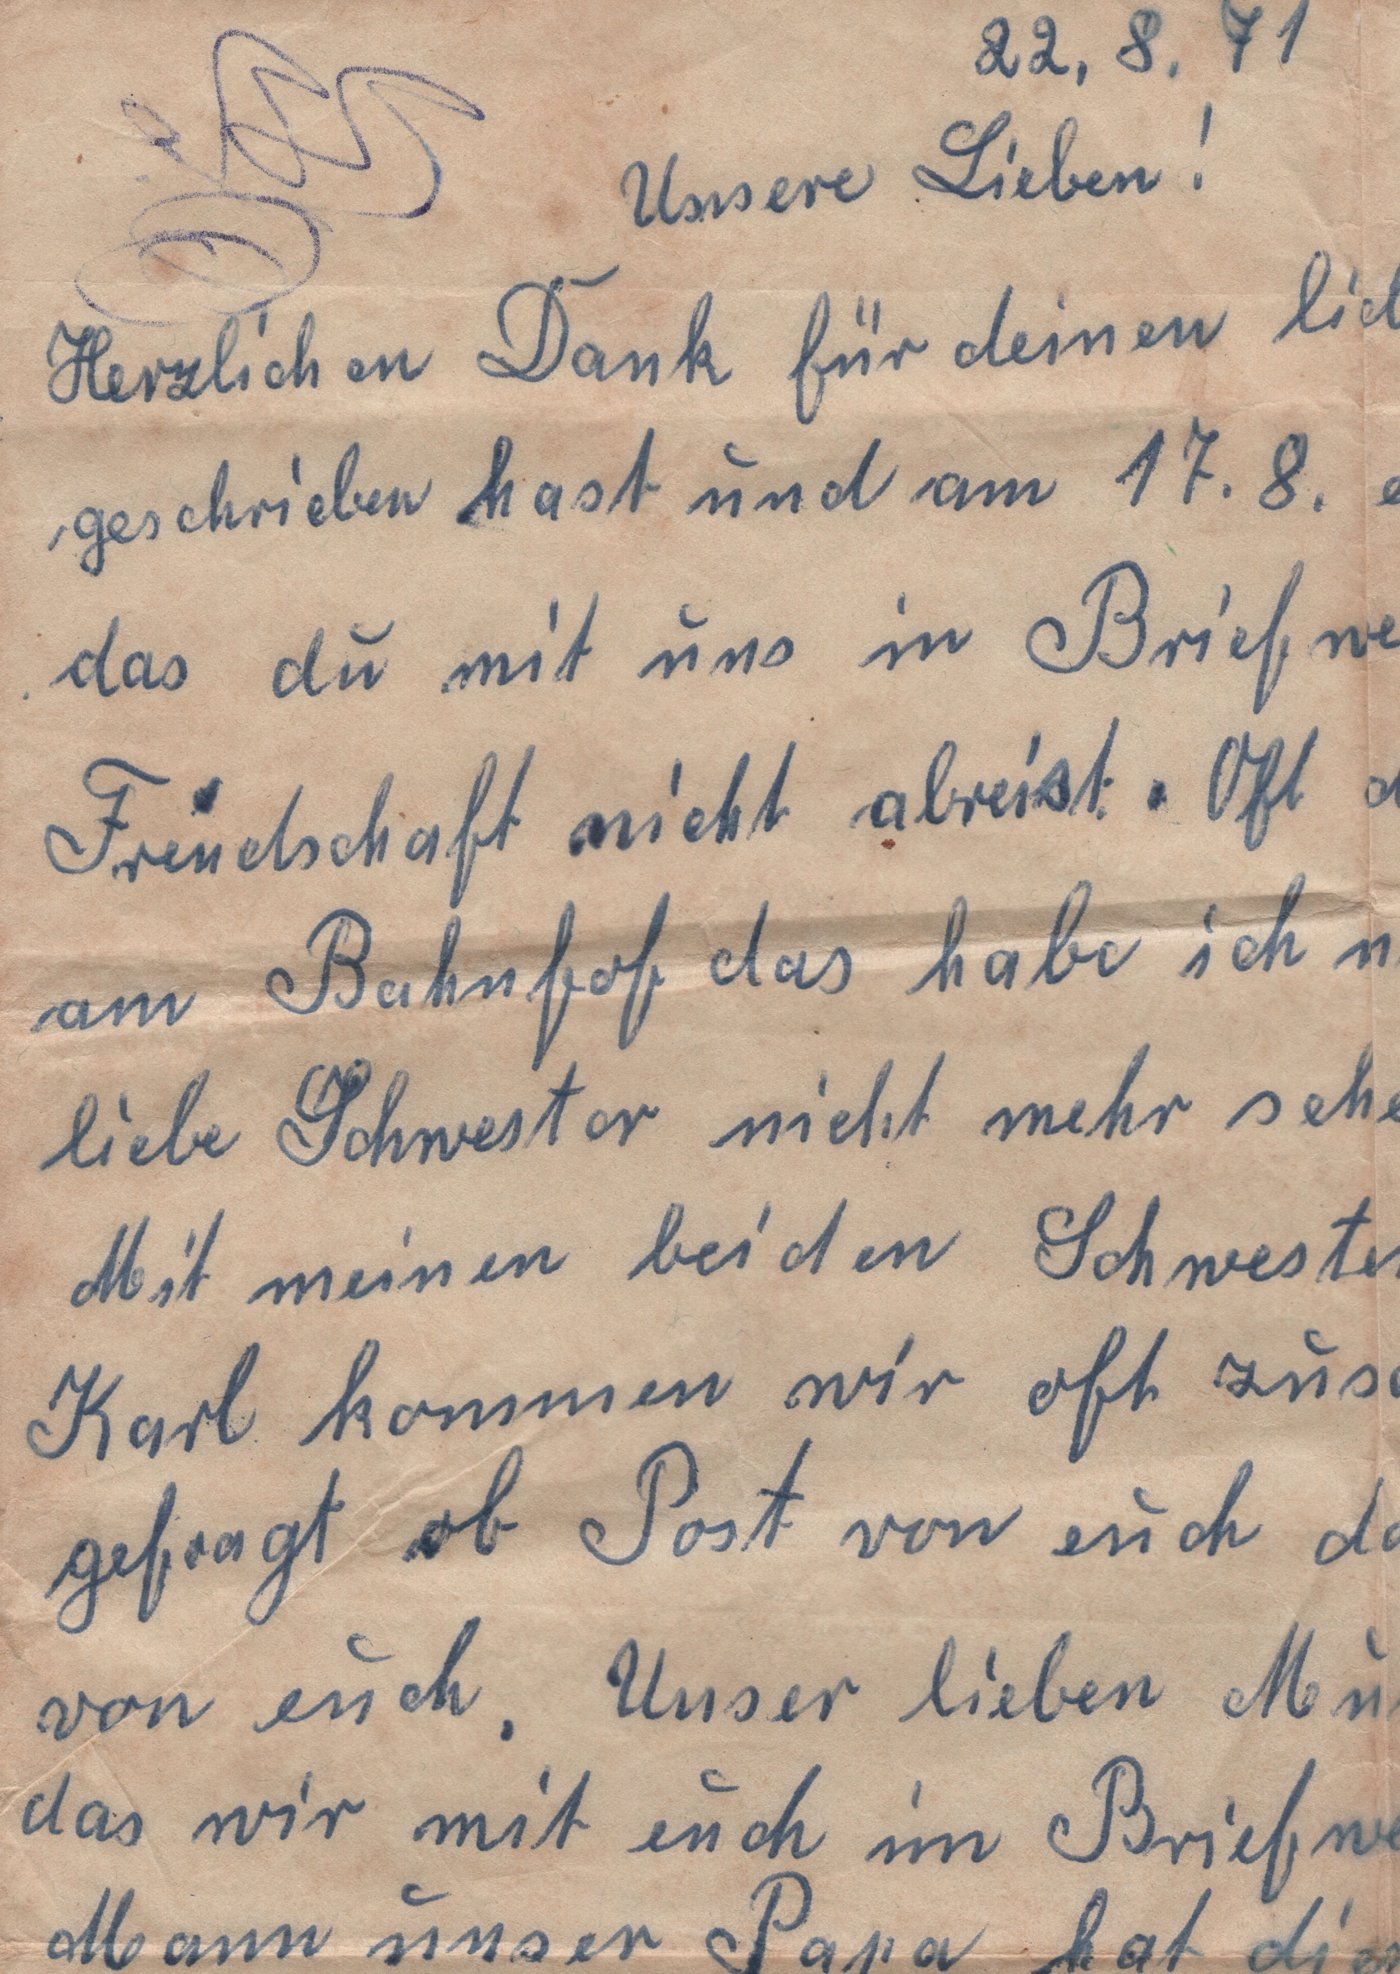
\includegraphics[width=0.75\linewidth,height=\textheight,keepaspectratio,alt={O começo da carta de 22 de agosto de 1971, escrita em Rempesgrün por uma irmã da Mota. Repare no pequeno arco sobre cada letra u. O lado direito da folha ficou fora do escaneamento.}]{imagens/carta_rempesgruen_1971.jpg}
\caption{O começo da carta de 22 de agosto de 1971, escrita em
Rempesgrün por uma irmã da Mota. Repare no pequeno arco sobre cada letra
\emph{u}. O lado direito da folha ficou fora do escaneamento.}
\end{figure}

A segunda carta, sem data visível, começa com \emph{Rempesg{[}rün{]}} e
foi escrita por outra mão, mais jovem. Diz que cada carta do Brasil é um
\emph{Freudentag}, um dia de festa; que já vão fazer quase sessenta anos
desde que se viram pela última vez, o que a põe por volta de 1972; que é
bom saber que todos cuidam bem da mãe e que ela recebe uma pequena
aposentadoria. Pergunta o nome e o endereço de alguém da família que
estaria na Alemanha Ocidental, e conta que o filho tem amigos em
Veszprém, na Hungria, e que a Hungria, como eles, é socialista.

A terceira tem data de 3 de janeiro de 197{[}4{]}, com o último
algarismo cortado, e foi escrita depois da morte da Mota, porque fala
dos \emph{pais que já não estão vivos}. Começa assim: \emph{Wir bedauern
das Ableben Eurer l{[}ieben{]} Mutter. Ihr Leben bestand aus M{[}ühe
und{]} Sorge. Es bleibt eben niemand auf {[}dieser{]} Erde.} Lamentamos
a morte da vossa querida mãe. A vida dela foi feita de trabalho e
preocupação. Ninguém fica para sempre nesta terra. Depois agradece à tia
Maria a carta e as fotografias, e explica, com uma franqueza que me fez
rir e quase chorar ao mesmo tempo, que ninguém ali conseguiu traduzir a
carta, porque tinha sido escrita em português, e lá as línguas eram o
alemão, o inglês e o russo. O tio Martin, diz, sempre lhes escreveu
cartas bonitas em alemão. E pede que, mesmo sem os pais vivos, a
correspondência não acabe: não precisam escrever cartas grandes, basta
que saibam sempre o que se passa do lado de cá.

A quarta é de novo da mulher do arco sobre o \emph{u}. Não tem data
visível. Ela conta que esperou muito por notícias e que precisa
comunicar que Walter, o marido dela, morreu. Estava cego e já não podia
andar. A última palavra dele, escreve, foi o nome dela, ou é assim que
leio a linha cortada. \emph{Es geht ein nach den andern}: vai um depois
do outro. Depois fala dos filhos, Hans e Horst, de uma casa bonita que
vão embelezando, e diz que tem três ovelhas.

Então a irmã da Mota era a mulher de Walter Heckel, e foi ela quem
escreveu de Rempesgrün. Não sei o nome dela. Pode ser Theresia, a irmã
nascida em Heumaden em 1890, ou uma irmã mais nova, nascida depois que a
família deixou a aldeia. O sobrenome de casada ela nos deu; o de
batismo, a carta guardou na metade que o escâner não pegou.

Quem manteve o fio, durante décadas, foi o tio Martin Sautner. A Mota
não escrevia em português, as filhas e os netos já não escreviam em
alemão, e era ele quem sentava à mesa em Ribeirão das Pacas e escrevia,
em alemão, para o outro lado da Cortina de Ferro. Quando a Mota morreu,
a família de lá soube. Mandou pêsames. Pediu para não parar.

E nós paramos. Não sei quando chegou a última carta, nem quem deixou de
responder. Sei que, quando comecei esta pesquisa, em 2012, ninguém me
falou dos primos de Rempesgrün, e que fui procurar parentes na Baviera,
onde eles não estavam. O mapa tinha um buraco, mas não era o buraco da
guerra: era o nosso. Antes de tentar fechá-lo, eu precisava recuar muito
mais. Minha mãe, Adelina Doerner, vinha de uma gente que tinha chegado a
Santa Catarina oitenta e cinco anos antes do \emph{Formosa}, em
veleiros, num tempo em que ainda não havia vapor nem quarentena de porto
em porto, mas havia calmaria. A estação seguinte desta retrotrajetória
fica na baía de Desterro, em novembro de 1828.

\section{Para vocês descobrirem}\label{para-vocuxeas-descobrirem-6}

\begin{itemize}
\tightlist
\item
  Qual neto ficava de vigia na estrada enquanto o rádio tocava no porão?
  Perguntem aos primos mais velhos.
\item
  O que o Fata queria em 1939: uma visita ou a volta definitiva? Havia
  passagem comprada ou só um desejo dito à mesa? Quem ouviu as versões
  daquele tempo pode ainda lembrar de alguma.
\item
  Por que caminho seguiram as caixas de 1945, e alguma resposta voltou
  da Alemanha?
\item
  Quais túmulos do cemitério de Aurora foram feitos pelo Fata? O texto
  do centenário não diz. Vão lá olhar e perguntem aos netos de Aurora.
\item
  Como se chamava a irmã da Mota casada com Walter Heckel? E quem eram
  as outras duas irmãs e o irmão Karl? As folhas inteiras das cartas,
  escaneadas em tamanho A4, frente e verso, devem trazer a assinatura.
\item
  Quem da família estava na Alemanha Ocidental por volta de 1972, a
  pessoa cujo endereço os primos de Rempesgrün pediram?
\item
  Onde estão as cartas que o tio Martin escreveu? Se os primos de lá as
  guardaram como nós guardamos as deles, elas contam o nosso lado da
  história.
\end{itemize}

\part{Os Pioneiros de 1828, o Mosela e as Lâminas de
Solingen}\label{os-pioneiros-de-1828-o-mosela-e-as-luxe2minas-de-solingen}

\begin{boletim}

Alísios de nordeste. Veleiros retidos na calmaria equatorial.
Visibilidade: quase dois séculos.

\end{boletim}

\chapter{12 de Novembro de 1828 --- Os Primeiros Barcos de
Desterro}\label{cap-8}

\begin{quote}
\emph{Antes do vapor, quem decidia a data da chegada era o vento.}
\end{quote}

\emph{49,7° N · 6,9° L, Hermeskeil, Hunsrück · 27,6° S · 48,8° O, São
Pedro de Alcântara, SC}

Não sei em que navio Anton Michels atravessou o oceano. A nota que
guardo sobre ele oferece duas rotas, com duas datas de chegada a
Desterro, separadas por cinco dias. Ignazia Loch, do mesmo ramo, tem
registro de nascimento num lugar que, no ano indicado, ainda não
existia. Bernard Preis tem um ano de nascimento no papel e outro na
pedra do túmulo.

Até aqui segui o lado do meu pai, que é o lado mais próximo e mais
documentado. Os Haas chegaram em 1913, e houve netos que ainda ouviram a
voz do \emph{Fata} contando histórias. Quando passo para o lado da minha
mãe, Adelina Doerner, a escala de tempo muda. Os Michels, os Arns e, ao
que parece, os Preiss e os Loch não chegaram a Santa Catarina num vapor
com manifesto datilografado e carimbo de porto. Chegaram em veleiros,
quase um século antes (os Doerner viriam depois, por outro caminho),
quando o Brasil ainda tinha imperador, a ilha de Santa Catarina se
chamava Desterro e não havia na província uma única colônia alemã.

O ramo materno, por isso, é feito de outro material. No lado Haas eu
tinha memória e procurava documentos. No lado Doerner tenho documentos,
muitos, espalhados por índices paroquiais, listas de navios e anotações
de genealogistas alemães e brasileiros, e quase nenhuma memória. Ninguém
viu Anton Michels desembarcar. Ninguém guardou a voz dele. O que tenho
são datas, umas certas e outras impossíveis, e grafias que mudam a cada
escrivão. Este capítulo é uma tentativa de pôr carne nesse esqueleto sem
fingir que ele é mais do que é.

\section{Hermeskeil, verão de 1828}\label{hermeskeil-veruxe3o-de-1828}

\emph{Hermeskeil, Hochwald do Hunsrück, Província do Reno (Prússia),
junho de 1828}

Anton Michels nasceu em 11 de maio de 1822 em Hermeskeil e foi batizado
no dia seguinte. Hermeskeil fica no Hochwald, a parte alta e florestada
do Hunsrück, uns trinta quilômetros a sudeste de Trier. Para um
meteorologista é um lugar fácil de imaginar: um planalto de meia
altitude, exposto aos ventos de oeste que chegam do Atlântico carregados
de umidade e a descarregam em forma de chuva fina, neblina e invernos
longos. Terra de centeio, aveia, batata e floresta, mais do que de
trigo. Uma terra que dava para viver se cada família tivesse o bastante
dela.

As famílias não tinham. Para entender por que um menino de seis anos
sobe a prancha de um navio em Bremen, é preciso entender uma regra
jurídica que nenhum dos meus antepassados leu, mas que todos eles
sofreram: a \emph{Realteilung}, a partilha igualitária. No Hunsrück, no
Mosela, em boa parte da Renânia e do Palatinado, a terra de um pai era
dividida em partes iguais entre todos os filhos quando ele morria.
Parece justo, e em certo sentido é, só que a cada geração os campos se
partiam de novo. Uma lavoura que sustentava uma família virava duas
faixas que sustentavam duas famílias pela metade, depois quatro tiras
que não sustentavam ninguém. No começo do século XIX havia aldeias do
Hunsrück em que um camponês trabalhava dez ou quinze retalhos de terra
espalhados pelo município, cada um do tamanho de um quintal. Na Baviera
antiga dos Haas valia o contrário, o herdeiro único, e os irmãos que não
herdavam viravam oleiros e operários. Aqui todos herdavam, e todos
herdavam pouco. São dois caminhos opostos para o mesmo resultado: gente
sobrando na terra.

A isso se somou o clima, e aqui o meteorologista pede licença. Em abril
de 1815 o vulcão Tambora, na Indonésia, teve uma das maiores erupções
dos últimos milênios. O véu de aerossóis de enxofre que subiu à
estratosfera espalhou-se pelo planeta e refletiu parte da luz do sol. O
ano seguinte, 1816, ficou conhecido na Europa como o ano sem verão:
geadas em junho, chuva sem fim, colheitas apodrecendo no campo. Na
Renânia e no sudoeste da Alemanha, 1816 e 1817 foram anos de fome. Anton
ainda não tinha nascido, mas nasceu numa região que lembrava daquela
fome e que tinha aprendido com ela que a terra podia falhar. A Renânia,
além disso, acabara de passar para o domínio da Prússia, depois do
Congresso de Viena, com impostos novos, serviço militar e uma
administração distante.

Foi nesse terreno que caíram as promessas dos agentes de emigração. Nos
anos 1820 o Império do Brasil, recém-independente, queria colonos
europeus para ocupar o Sul e defendê-lo, e mandava recrutá-los na
Alemanha. Os recrutadores falavam de terra de graça, de ferramentas, de
sementes, de subsídio nos primeiros anos. Imagino que no inverno de 1827
para 1828 essas palavras tenham corrido as aldeias do Hochwald de casa
em casa. Imagino também a decisão dos pais de Anton. Seus nomes não
consegui fixar com segurança nas fontes que tenho, e eles aparecem aqui
só como ``os pais''. Vendem o pouco que têm e partem com os filhos para
Bremen, no verão de 1828, para atravessar o oceano.

Para um menino de seis anos a viagem até o porto já devia ser a maior
aventura da vida. Primeiro as estradas do Hunsrück, depois os rios,
depois a planície do norte, que ele nunca tinha visto, sem colinas e sem
florestas, com um céu enorme. Bremen, os mastros, o cheiro de alcatrão.
É provável que ele não entendesse a palavra \emph{Brasilien}. Entendia
que estava indo com a família para algum lugar, e para uma criança isso
basta.

\section{Duas rotas para um mesmo
novembro}\label{duas-rotas-para-um-mesmo-novembro}

\emph{Bremen, junho e julho de 1828}

A primeira dúvida aparece logo no cais. O perfil de Anton Michels no
FamilySearch guarda, nas notas, um resumo compilado de fontes alemãs que
reproduzo aqui porque é a melhor descrição que tenho da viagem e porque
mostra, com franqueza, que não se sabe em qual navio ele veio.

\begin{ficha}

\textbf{Ficha do Arquivo}: Nota no perfil de Anton Michels no
FamilySearch (LDL7-7XZ), em alemão, com referência à compilação
\emph{Emigration nach Brasilien 1828}, de Ursula Buchholz. Tradução
livre: ``Em 7 de novembro de 1828, 276 pessoas chegaram com o
\emph{Luiza} à colônia de São Pedro de Alcântara. Em 12 de novembro de
1828 chegaram com o \emph{Marquês de Viana} outras 259 pessoas. Destas,
523 colonos vieram diretamente de Bremen (Bremerhaven). Entre eles,
gente dos distritos de Cochem, Mayen, Bernkastel-Wittlich e
Trier-Saarburg.'' Seguem duas rotas possíveis: de Bremen, em 28 de junho
de 1828, no \emph{Johanna Jakobs}, até o Rio de Janeiro, e dali, em
outubro, no \emph{Luiza}, até Desterro (chegada em 7 de novembro); ou de
Bremen, em 6 de julho de 1828, no \emph{Charlotte \& Louise}, até o Rio,
e dali, em outubro, no \emph{Marquês de Viana}, até Desterro (chegada em
12 de novembro). A data de imigração registrada para Anton é 12 de
novembro de 1828.

\end{ficha}

A nota diz ``oder'', ou. A data que ficou no registro de Anton, 12 de
novembro, é a da chegada do \emph{Marquês de Viana}, e por ela ele teria
saído de Bremen no \emph{Charlotte \& Louise}. Mas a mesma nota oferece
a outra rota, o \emph{Johanna Jakobs} e o \emph{Luiza}, chegando cinco
dias antes, e foi essa a primeira versão que entrou nas minhas anotações
e no roteiro deste livro. Não tenho como decidir. Para isso precisaria
ver as listas de passageiros com o nome dele, e não as vi. Fico com o 12
de novembro, que é a data registrada, mas mantenho a outra rota viva. Em
genealogia, como em previsão do tempo, é melhor publicar a incerteza do
que uma certeza falsa.

Há outro detalhe nesses números. Dos 535 que chegaram nos dois brigues,
523 vinham direto de Bremen; os demais, imagino, juntaram-se no caminho,
no Rio de Janeiro. E as regiões de origem citadas, Cochem, Mayen,
Bernkastel-Wittlich e Trier-Saarburg, desenham no mapa um único
território: o Mosela e o Hunsrück, a margem esquerda do Reno. Os
pioneiros de São Pedro de Alcântara eram, em grande parte, vizinhos.
Saíram das mesmas colinas, falavam o mesmo dialeto e tinham fugido da
mesma partilha. Há registro, por exemplo, de uma família Berens, de
Wintrich, no Mosela, que chegou no brigue \emph{Luiza} em 7 de novembro
de 1828 e se instalou na nova colônia.\footnote{A família Berens
  (Berns), de Wintrich, Bernkastel-Wittlich, é citada por Toni Jochem
  como chegada no brigue \emph{Luisa} em 7 de novembro de 1828 e
  instalada em São Pedro de Alcântara. Ver o artigo de Toni Jochem e
  colaboradores sobre as colônias Piedade e Santa Isabel, na série
  \emph{Páginas da Colonização: Estudos/subsídios históricos sobre a
  Colônia Alemã Santa Isabel --- 175 anos de Fundação} (2022--2023).}

\section{Calmaria}\label{calmaria}

\emph{Atlântico, entre o Canal da Mancha e o Rio de Janeiro, julho a
setembro de 1828}

Não sei quanto durou a travessia de Anton, mas sei como eram essas
viagens, e sei como era o oceano que ele cruzou, porque é o mesmo de
hoje. Um veleiro que saía de Bremen no começo de julho descia o Mar do
Norte, passava o Canal, ganhava o Atlântico e procurava os alísios de
nordeste, que o empurravam para o sul e o sudoeste com regularidade de
relógio. Até aí, com sorte, a viagem andava.

Depois vinha a faixa que os marinheiros temiam e que eu ensino aos
alunos com outro nome. Perto do equador os alísios dos dois hemisférios
se encontram, o ar sobe, forma nuvens altas e pancadas de chuva, e na
superfície o vento simplesmente some. Hoje chamamos essa faixa de Zona
de Convergência Intertropical. Os marinheiros ingleses a chamavam de
\emph{doldrums}, e os portugueses, de calmarias. Um navio podia ficar
ali parado dias, às vezes semanas, com as velas penduradas, sob um calor
úmido que não dá trégua, esperando um sopro que o tirasse do lugar. A
água doce apodrecia nos barris, a comida estragava, as crianças
adoeciam. É o ponto da viagem em que se entende que, antes do vapor,
quem decidia a data da chegada era o vento.

Imagino Anton, aos seis anos, no convés de um navio parado no meio do
oceano. Talvez achasse aquilo bonito, a água lisa como um espelho e o
horizonte em toda a volta. Talvez visse um enterro no mar, porque em
quase toda travessia daquele tempo alguém morria, e quase sempre eram as
crianças e os velhos. Não sei se a família dele perdeu alguém. Sei que
ele sobreviveu. Num navio de emigrantes de 1828, que um menino de seis
anos sobrevivesse era um acontecimento.

Passada a calmaria, os alísios de sudeste levavam o navio ao longo da
costa brasileira até o Rio de Janeiro. Ali os colonos esperavam,
desembarcavam, eram contados e redistribuídos. Em outubro de 1828 os
destinados a Santa Catarina embarcaram nos dois brigues costeiros, o
\emph{Luiza} e o \emph{Marquês de Viana}, para a última perna da viagem,
para o sul, ao longo de uma costa de serras verdes que nenhum deles
conhecia.

\section{Uma vila açoriana e uma estrada para
Lages}\label{uma-vila-auxe7oriana-e-uma-estrada-para-lages}

\emph{Nossa Senhora do Desterro, novembro de 1828 a março de 1829}

O brigue entrou na baía de Desterro numa manhã de novembro. Se foi mesmo
o \emph{Marquês de Viana}, era 12 de novembro de 1828. É a data que dá
título a este capítulo, e gosto dela também pelo que tem de incerto,
como uma observação que pode estar cinco dias errada.

Para um menino do Hunsrück aquilo devia ser outro planeta. A ilha
coberta de mata, a água morna da baía, as casas brancas de uma vila de
pescadores e lavradores de origem açoriana, que falavam uma língua que
ele não entendia e professavam a mesma fé que ele, embora rezassem de
outro jeito. Os moradores de Desterro tampouco sabiam o que fazer com
aquela gente de cabelo claro e roupa de lã. Uma vila acostumada à
farinha de mandioca e ao peixe recebia de uma vez mais de quinhentos
colonos alemães para alojar e alimentar enquanto o governo decidia onde
pô-los.

Há uma coisa que o meteorologista não pode deixar passar. O roteiro
deste livro, numa primeira versão, falava do ``inverno de espera'' em
Desterro. Era um erro de hemisfério. Anton chegou em novembro, no fim da
primavera austral, e passou em Desterro o verão, o primeiro verão da
vida dele em que dezembro foi quente. A família, que deixara Bremen no
verão do norte, emendou dois verões e pulou um inverno inteiro. Gosto de
pensar que o menino estranhou o Natal com calor e os dias longos de
janeiro, e que em algum momento daquele verão aprendeu a palavra ``mar''
em português.

A espera durou alguns meses. Em março de 1829 os colonos foram levados
para o continente e subiram em direção à serra, ao longo da estrada que
o governo abria para ligar Desterro a Lages, no planalto. Ali, a uns
trinta quilômetros da costa, foi fundada a colônia de São Pedro de
Alcântara, a primeira colônia alemã de Santa Catarina. A ideia era
povoar a estrada, para que os tropeiros e as tropas tivessem pouso,
comida e gente ao longo do caminho, e ao mesmo tempo ocupar terras que o
Império considerava vazias.

Não estavam vazias, mas essa é uma conversa que já começou no Capítulo 6
e que não cabe repetir aqui. Estavam também longe de ser boas. As
encostas de São Pedro de Alcântara eram íngremes, o solo pobre e lavado
pela chuva, e as promessas de subsídio e ferramentas, como aconteceria
com os Haas oitenta e cinco anos depois em Rio do Ouro, foram cumpridas
pela metade ou não foram. Nos anos seguintes muitas famílias abandonaram
a colônia e se espalharam pelos vales vizinhos, por Santo Amaro, pela
baixada, por onde houvesse terra que desse. Anton Michels acompanhou
esse movimento. Quando o reencontramos nos registros, já homem, ele vive
na Colônia Santa Isabel, fundada em 1847 mais acima na mesma estrada de
Lages. Morreu em 1874 em Vargem Grande, hoje município de Águas Mornas.
Entre o menino do brigue e o colono de Santa Isabel há quase vinte anos
de que não sei nada. O próximo capítulo começa quando a vida dele cruza
a de uma moça do Mosela.

\section{Ignazia, a menina sem data}\label{ignazia-a-menina-sem-data}

\emph{São Pedro de Alcântara, 1828?}

No mesmo ramo da árvore, duas gerações acima de Gertrudes Preiss, minha
avó materna, há um casal que também pertence a essa primeira leva, ou
que pelo menos deveria pertencer. São Bernard Preis e Ignazia Loch, pais
de Emanuel Preis, meu bisavô, que o recenseamento de 1920 chamará de
Manoel Preuss. Para Ignazia o registro diz o seguinte.

\begin{ficha}

\textbf{Ficha do Arquivo}: Perfil de Agnes Ignacia (Ignazia) Loch no
FamilySearch (LV7G-Z2H). Nascimento: ``1828, São Pedro de Alcântara,
Santa Catarina, Brasil''. Falecimento: ``von 1872 zu 1914'', ou seja, um
intervalo estimado, sem data. Nos índices paroquiais e civis
catarinenses em que aparece como mãe ou avó, o nome dela é grafado
Ignacia Loch, Ignazia Locho, Ignacia Lock, Ignacia Locks, Ignazia Luch,
Ignacia Roch e até Ignácio Lach.

\end{ficha}

Esse registro tem um problema que se vê à primeira leitura. Ignazia não
pode ter nascido em São Pedro de Alcântara em 1828, porque em 1828 São
Pedro de Alcântara não existia. Os colonos chegaram a Desterro em
novembro daquele ano e a colônia só foi assentada em março de 1829. Uma
data e um lugar que não podem coexistir são, para quem trabalha com
dados, o equivalente a uma estação que registra neve em Florianópolis em
pleno janeiro: alguma coisa foi anotada errado, e é preciso descobrir o
quê.

Vejo quatro possibilidades. A primeira é que Ignazia tenha nascido na
Europa em 1828, antes da partida, e chegado de colo num daqueles
brigues. Nesse caso o lugar está errado e o ano, certo. A segunda é que
tenha nascido a bordo, durante a travessia ou na espera do Rio, o que
acontecia com frequência e explicaria por que alguém, mais tarde,
atribuiu o nascimento ao único lugar brasileiro que a família conhecia.
A terceira é que tenha nascido em Desterro, entre novembro de 1828 e
março de 1829, durante a espera, e que a memória familiar tenha fundido
a cidade da espera com a colônia que veio depois. A quarta é que o ano
seja apenas aproximado, um ``por volta de 1828'' que virou data, e que
ela tenha nascido já na colônia, em 1829 ou depois.

A quarta me parece a mais provável, mas não tenho como prová-la.
Emanuel, o filho dela que nos interessa, nasceu em 1864, e há filhos
batizados até 1872. Se Ignazia nasceu em 1828, teria 44 anos no último
parto, o que é possível, mas raro. Alguns anos a menos tornariam tudo
mais comum. É só uma probabilidade, e uma probabilidade não substitui um
assento de batismo. Por isso, ao longo deste livro, a data de nascimento
de Ignazia Loch é tratada como aproximada.

O sobrenome também não ajuda tanto quanto eu gostaria. Loch é nome do
Mosela e do Hunsrück, como quase todos os desta parte da árvore. Aparece
na tradição de São Pedro de Alcântara e aparece também na lista de
sobrenomes da Colônia Santa Isabel, de 1847 em diante. No recenseamento
de 1920 há um Pedro Loch Junior proprietário na mesma página que Manoel
Preuss, no vale do Capivari. Os Loch e os Preis, em outras palavras,
viveram lado a lado por pelo menos três gerações, e eu ainda não sei
dizer de qual leva de navios saiu a família de Ignazia.

\section{O homem de Schweich}\label{o-homem-de-schweich}

\emph{Schweich, Mosela, 1827 (ou 1829)}

Bernard Preis é, se possível, ainda mais escorregadio. O arquivo diz que
nasceu em 1827 em Schweich, uma pequena cidade à beira do Mosela, poucos
quilômetros rio abaixo de Trier, terra de vinhedos em encosta e de
barqueiros. Ao lado dessa data, porém, há uma nota de outra mão.

\begin{ficha}

\textbf{Ficha do Arquivo}: Perfil de Bernhard (Bernard) Preiss no
FamilySearch (L58N-QCC). Nascimento: 1827, Schweich, Trier, Renânia,
Prússia. Nota anexa: ``No túmulo consta na lápide a data de 1829.''
Falecimento: 11 de outubro de 1893, Alto São Martinho, Santa Catarina.
Nos índices brasileiros em que aparece como pai, o nome é grafado
Bernard Preis, Bernardo Preis, Bernard Preus, Bernardo Reis, Bernardo
Freis, Bernardo Treis e Bernardo Redo.

\end{ficha}

O registro de papel diz 1827; a pedra do túmulo, 1829. Uma lápide
costuma ser feita pelos filhos, que sabem a idade do pai de ouvido, e um
registro genealógico costuma ser montado a partir de um batismo, que é
mais confiável, ou de uma idade declarada num óbito, que é menos. Sem
ver o batismo de Schweich, não tenho como arbitrar. Fico, como no caso
de Ignazia, com a data do arquivo e a ressalva ao lado.

A dúvida maior é outra: quando e como Bernard chegou ao Brasil. Não sei.
Se nasceu em 1827, poderia ter vindo de colo na leva de 1828, o que
faria dele companheiro de viagem de Anton Michels sem que nenhum dos
dois soubesse que os filhos se casariam. Poderia também ter vindo jovem,
na segunda grande onda, a de 1846 e 1847, que trouxe a família Arns e
fundou Santa Isabel. Ou mais tarde, sozinho. Há uma pista solta que
anoto por honestidade, sem lhe dar mais peso do que tem. Na planta da
Colônia da Piedade, de 1850, reconstituída pelo pesquisador Beat Richard
Meier e citada pelo historiador Toni Jochem, aparece um lote de um certo
Sebastian Preis, vizinho de famílias que chegaram em janeiro de
1847.\footnote{Mesma fonte da nota anterior, que se apoia em Beat
  Richard Meier (1990) e na planta da Colônia Alemã de Nossa Senhora da
  Piedade, de 1850. A relação de Sebastian Preis com Bernard Preis é
  apenas uma hipótese a investigar.} Seria um parente de Bernard, um
pai, um tio, um irmão mais velho? Ou apenas um homônimo, como tantos que
já me fizeram perder semanas? Por ora é um ponto no mapa, sem seta
ligando-o a nada.

O que se sabe com segurança vem depois, já no Brasil. Em 1864 Bernard e
Ignazia vivem na Colônia Vargem Grande, ao lado de Santa Isabel, hoje
Águas Mornas. Ali nasce, em 31 de março, o filho Emanuel, batizado em 26
de abril do mesmo ano com o nome de Manuel. Vêm depois, entre outros,
Nicolaus, batizado em 1868, Peter, em 1870, e Johannes, em 1872. É a
mesma Vargem Grande onde Anton Michels morreria em 1874, e a mesma
vizinhança em que, ao que tudo indica, nasceu Helena Michels, filha de
Anton, no mesmo ano de 1864 que Emanuel. Os dois bebês de 1864, ela
filha de um pioneiro de 1828 e de uma imigrante de 1847, ele filho de um
homem de Schweich cuja chegada ninguém registrou, cresceram
provavelmente a poucos quilômetros um do outro, sem que ninguém pudesse
imaginar que seriam meus bisavós.

Mais tarde os Preis, como os Michels, desceram para o sul, para os vales
do Capivari, em São Martinho, onde havia terra nova. Bernard morreu ali,
em Alto São Martinho, em 11 de outubro de 1893, com cerca de 66 anos se
a data do papel estiver certa, cerca de 64 se a da pedra estiver. A essa
altura o sobrenome já começava a se desfazer na boca dos escrivães
brasileiros. Preis virou Preiss, virou Preuss, virou Reis, Freis, Treis.
Num índice há até o casamento de uma filha dele datado de 1809, quase
vinte anos antes de existir qualquer Preis em Santa Catarina, prova de
que o erro de digitação também é uma força da natureza. Minha avó será
registrada como Gertrudes Preuss e conhecida como Gertrudes Preiss.
Neste livro, por convenção, uso Preis para Bernard e Emanuel, que é como
aparecem nos registros mais antigos, e Preiss para Gertrudes, como a
família a chamava. São a mesma gente com a ortografia que cada escrivão
conseguiu.

Penso em Bernard de Schweich e em Anton de Hermeskeil como dois homens
vindos da mesma lógica. Os dois nasceram na margem esquerda do Reno, a
pouco mais de vinte quilômetros um do outro, em terras onde a partilha
igualitária tinha retalhado os campos até o osso. Os dois deixaram o
Mosela e o Hunsrück para receber, do outro lado do mundo, um lote
inteiro, um pedaço de terra que nenhum irmão ia dividir. Do lote
prometido de 1828 ao ``lote'' que agora tento entregar aos meus filhos
em forma de arquivo digital, a palavra atravessa este livro. Aqueles
homens cruzaram o oceano para não ter de partir a terra em pedaços. Os
filhos deles, com dez, doze, quinze irmãos cada um, logo descobririam
que no Brasil a conta também não fechava, e que o remédio era o mesmo:
partir de novo, mais para o sul, mais para o interior.

Dezenove anos depois daquele novembro de 1828, outro brigue entrou na
baía de Desterro. Trazia, entre os passageiros, uma moça de dezenove
anos nascida numa curva do Mosela. Ela viveria quase um século.

\section{Para vocês descobrirem}\label{para-vocuxeas-descobrirem-7}

\begin{itemize}
\tightlist
\item
  Em qual rota veio Anton Michels: no \emph{Johanna Jakobs} e depois no
  \emph{Luiza}, ou no \emph{Charlotte \& Louise} e depois no
  \emph{Marquês de Viana}? Só as listas de passageiros com o nome dele
  podem dizer, e eu não as vi.
\item
  Onde e quando nasceu Ignazia Loch, e de qual leva de navios saiu a
  família dela? Um assento de batismo valeria mais do que todas as
  minhas probabilidades.
\item
  Quem era Sebastian Preis, dono de um lote na planta da Colônia da
  Piedade de 1850: parente de Bernard ou apenas homônimo?
\item
  Bernard Preis nasceu em 1827, como diz o arquivo, ou em 1829, como diz
  a lápide? E quando chegou ao Brasil? Comecem pelo batismo de Schweich,
  que eu não vi.
\end{itemize}

\chapter{A Matriarca de 96 Anos --- De Pünderich ao Lote
38}\label{cap-9}

\begin{quote}
\emph{Há rios que fazem curvas tão fechadas que quase se encontram
consigo mesmos. Certas vidas também.}
\end{quote}

\emph{50,0° N · 7,1° L, Pünderich, Mosela · 28,1° S · 48,9° O, Vargem do
Cedro, São Martinho, SC}

Durante cinco meses de 1924, uma mulher nascida em 1827 e um bebê
dividiram o mesmo céu catarinense. Os dois nunca se viram e ninguém
pensou neles juntos. O bebê era Baldoíno Haas, meu pai. A mulher, a que
viveu mais que todas as outras na árvore da família, é a razão de este
capítulo se chamar assim. Angela Catharina Arns nasceu em dezembro de
1827 na margem do Mosela e morreu em setembro de 1924 num vale do sul de
Santa Catarina, a menos de três meses de completar 97 anos. Atravessou o
oceano aos dezenove, ficou viúva aos quarenta e seis, mudou de vale com
os filhos e enterrou, é quase certo, gente demais.

Nos registros ela muda de nome conforme a mão que escreve. É Angela
Catharina Arend no FamilySearch, mas nos índices paroquiais e civis
aparece como Catharina Arns, Catharina Arens, Catarina Arns, Cathar.
Arns, Catharina Arno e, num índice de 1849, num desses desastres de
transcrição que eu já aprendi a amar, como Angela Catharina Armando. Uso
Arns, porque é assim que a família a chama hoje e é assim que o pai,
Nikolaus, aparece nas listas da colônia. Arend, a forma que está no
FamilySearch, é provavelmente a grafia alemã de origem. Os escrivães
brasileiros do século XIX escreviam os sobrenomes alemães como os
ouviam, e cada ouvido ouvia uma coisa. Para quem pesquisa, antes de
cruzar os dados, é preciso descobrir que se trata da mesma pessoa.

\section{Uma curva do Mosela}\label{uma-curva-do-mosela}

\emph{Pünderich, Mosela, Província do Reno (Prússia), 5 de dezembro de
1827}

Pünderich fica numa das curvas mais fechadas do Mosela, perto de Zell. O
rio, que desce da França rumo a Koblenz, ali se dobra sobre si mesmo num
laço, de modo que a aldeia, de um lado, olha para as encostas de vinhedo
do outro. Quem já viu fotografias do Mosela conhece a paisagem: aldeias
de casas de enxaimel espremidas na margem, igrejas de torre pontuda e,
por cima de tudo, as encostas de ardósia tão íngremes que as videiras
parecem penduradas.

Esse vale é uma lição de microclima, e eu não resisto a ela. A uva não
deveria amadurecer tão ao norte. O Mosela está a cinquenta graus de
latitude, muito ao norte para uma uva. Só amadurece porque o vale é
fundo e protegido do vento, porque as encostas viradas para o sul
recebem o sol de frente, quase em ângulo reto, e porque a ardósia escura
guarda o calor do dia e o devolve à noite, como um acumulador. Há ainda
o rio, que, largo, reflete luz e amortece as geadas. O vinhedo do Mosela
é um equilíbrio de frações de grau. Um ano de verão curto ou de geada
tardia basta para estragar a colheita.

Foi nesse lugar, no começo do inverno de 1827, que Angela Catharina
nasceu, filha de Nikolaus Arns. Foi batizada na igreja de Maria
Himmelfahrt, a igreja da Assunção da aldeia. Quando a família emigrou,
vinte anos depois, Nikolaus viajou com a ``segunda esposa'', Maria
Elisabetha Klering. Por muito tempo só deduzi que a primeira,
provavelmente a mãe de Angela, tinha morrido antes de 1847. O
FamilySearch traz um nome: Anna Margaretha Simonis, nascida em Reil em
1802, casada com Nikolaus em Pünderich em 27 de novembro de 1821 e morta
em Pünderich em 3 de fevereiro de 1835, quando Angela tinha sete anos.
Ainda preciso conferir esses dados nos livros da paróquia. Se estiverem
certos, Angela cresceu com uma madrasta e atravessou o oceano ao lado
dela. Não há nos documentos uma linha sobre como era essa relação. Fica
registrado apenas que a moça que embarcou para o Brasil já tinha perdido
alguém.

Imagino a infância dela pelo pouco que se sabe das aldeias do Mosela
naqueles anos: o trabalho nos vinhedos desde cedo, a colheita de outono
com cestos nas costas, encosta acima e encosta abaixo, a missa, o
dialeto. Imagino também a terra encolhendo. A mesma partilha igualitária
que retalhou os campos do Hunsrück, no capítulo anterior, retalhava os
vinhedos do Mosela. Uma parreira a mais ou a menos fazia diferença.
Quando um vinhedo é dividido entre seis filhos, cada um herda umas
poucas fileiras de videiras numa encosta onde só se sobe a pé.

\section{O brigue sardo}\label{o-brigue-sardo}

\emph{De Pünderich a Desterro, 1846 a 5 de janeiro de 1847}

Em 1845 apareceu nos campos da Europa uma doença que ninguém conhecia.
As folhas da batata escureciam, os tubérculos apodreciam na terra, e em
poucas semanas lavouras inteiras se perdiam. Era o míldio da batata, um
micro-organismo trazido das Américas que gostava exatamente do clima
úmido e ameno do noroeste europeu. Na Irlanda provocou a Grande Fome. Na
Renânia e no Mosela, onde a batata tinha se tornado o pão dos pobres, os
anos de 1845 a 1847 foram de colheitas perdidas, preços em disparada e
fome, agravados por safras ruins de cereais em 1846. Para uma família
que vivia de poucas fileiras de videiras e de uma horta de batatas, foi
o empurrão final.

Foi nessa crise que se formou a segunda grande onda de emigração alemã
para o Brasil, a de 1845 a 1847, que fundou Petrópolis, no Rio de
Janeiro, e, em Santa Catarina, as colônias de Santa Isabel e da Piedade.
Os navios saíam de Dunquerque, de Antuérpia, de Hamburgo. Não sei de que
porto saiu a família Arns. Sei em que navio fez a travessia oceânica e
em que barco chegou a Desterro, porque o perfil dela no FamilySearch
guarda uma nota que é, até hoje, o documento mais preciso que tenho
sobre esse ramo.

\begin{ficha}

\textbf{Ficha do Arquivo}: Nota de imigração no perfil de Angela
Catharina Arns (Arend) no FamilySearch (L61J-RDG), apoiada, segundo
outra nota do mesmo registro, num livro de história da família Michels
no Brasil: ``Nikolaus Arns veio da Europa a bordo do brigue sardo
\emph{Eridano}, com a segunda esposa, Maria Elisabetha Klering, e os
filhos Anna Bárbara, Ângela Catharina, Phillipp Joseph e Anna Maria.
Chegaram a Desterro (atual Florianópolis), Santa Catarina, em
05/01/1847, a bordo da sumaca \emph{14 de Novembro}. Fizeram parte da
segunda leva de imigrantes para a Colônia Santa Isabel e foram enviados
para a localidade de Primeira Linha Velha (que posteriormente passou a
ser chamada Loeffelscheidt), Rio dos Bugres. Receberam o lote número
38.''

\end{ficha}

Um brigue sardo, isto é, com bandeira do Reino da Sardenha, cujo porto
principal era Gênova. Os estudos que o historiador Toni Jochem reuniu
para os 175 anos de Santa Isabel confirmam o desenho dessa viagem em
duas pernas. Os imigrantes que formaram Santa Isabel e a vizinha Colônia
da Piedade chegaram ao Rio de Janeiro no fim de 1846, em navios como a
galera americana \emph{Ariosta} e o brigue sardo \emph{Eridano}. Do Rio
foram redistribuídos em barcos costeiros: o \emph{Vênus} e o \emph{14 de
Novembro} levaram os que iriam para Santa Isabel; o \emph{Affonso I} e a
corveta \emph{Bertioga}, os da Piedade.\footnote{Toni Jochem e
  colaboradores, série \emph{Páginas da Colonização: Estudos/subsídios
  históricos sobre a Colônia Alemã Santa Isabel --- 175 anos de
  Fundação} (2022--2023), em especial a introdução e o artigo sobre as
  colônias Piedade e Santa Isabel, que retoma a pesquisa de Beat Richard
  Meier (1990) e a Coleção Ficker. As datas de 16 de julho de 1847
  (primeiras certidões de demarcação) e a citação do jornal \emph{O
  Conciliador Catharinense} (1850) vêm desses textos.} Na reconstituição
de um desses pesquisadores, as duas colônias nasceram juntas porque
nenhuma delas tinha lotes bastantes para acomodar todos os colonos
chegados entre o fim de 1846 e o início de 1847. Dividiram-nos pelos
navios que os traziam.

Não tenho como reconstituir a travessia de Angela com mais do que
imaginação, e é com ela que escrevo o que segue. A moça tinha dezoito
anos quando embarcou. Viajava com o pai, que já não era jovem, com a
madrasta e com três irmãos, e é provável que coubesse a ela, como irmã
mais velha ou quase, uma parte do cuidado com os pequenos. Phillipp
Joseph e Anna Maria, pela ordem em que a nota os lista, eram os mais
novos. Um brigue de emigrantes não tinha cabines para ninguém. As
famílias dormiam no entrepont, entre caixotes e trouxas, com pouca luz e
pouco ar, e o enjoo das primeiras semanas devia ser seguido pelo tédio,
pelo calor do equador, pela calmaria que já descrevi no capítulo
anterior. O aniversário dela caía em 5 de dezembro. Se as datas que
conhecemos estão certas, completou dezenove anos no mar, ou na espera do
Rio de Janeiro, ou num barco costeiro descendo para o sul. Imagino que
ninguém tenha feito festa. Imagino também que alguém, a madrasta talvez,
tenha lembrado da data, porque nas famílias católicas do Mosela o dia do
santo e o dia do nascimento não passavam em branco. É um detalhe que
nenhum documento confirma e que eu me permito por ser o único presente
que posso dar a ela.

Angela tinha acabado de fazer dezenove anos quando a sumaca entrou na
baía. Era 5 de janeiro, pleno verão. Pela segunda vez, no espaço deste
livro, uma família do Mosela ou do Hunsrück chega a Desterro na estação
quente, depois de deixar a Europa no frio, e eu penso no choque térmico
daquele janeiro, no ar pesado da baía, na roupa de lã que não servia
para nada. Penso também numa coincidência que nenhum deles podia
conhecer. Dezenove anos antes, na mesma baía, tinha desembarcado de
outro brigue um menino de Hermeskeil chamado Anton Michels.

\section{Lote 38}\label{lote-38}

\emph{Primeira Linha, Rio dos Bugres, Colônia Santa Isabel, 1847 a 1874}

A Colônia Santa Isabel não tem data exata de fundação, e o próprio Toni
Jochem, que dedicou anos a ela, diz isso com todas as letras. Sabe-se
que em maio de 1847 o nome já aparecia num relatório do governo imperial
e que as primeiras certidões de demarcação dos lotes foram expedidas em
16 de julho de 1847. Um jornal de 1850 diz que a colônia ``teve
princípio em julho de 1847''. Fica no caminho entre Desterro e Lages, a
mesma estrada que, duas décadas antes, os colonos de São Pedro de
Alcântara tinham sido postos a povoar, só que mais acima, já na subida
da serra, nas terras do que hoje são os municípios de Águas Mornas e
Rancho Queimado.

A família Arns foi para a Primeira Linha, a linha colonial aberta em
1847 ao longo do Rio dos Bugres, que mais tarde ganharia o nome de
Loeffelscheidt. O nome lembra Löffelscheid, uma aldeia das colinas acima
do Mosela, e é provável que tenha vindo de colonos que saíram de lá.
Recebeu o lote número 38. É um número pequeno e eu me apeguei a ele mais
do que deveria, porque é a primeira propriedade da família na América de
que tenho registro: um retângulo de mata na encosta, com frente para um
rio de nome que hoje ninguém usaria.

O mesmo jornal de 1850 descreve a colônia em poucas linhas que valem
como fotografia. Diz que já tinha mais de setenta pessoas, que havia
abundância de pastos, animais e plantações e que cada família tinha seu
engenho de farinha e também de açúcar. Diz ainda que a colônia tinha
``um ramo na várzea grande''. Essa várzea grande, imagino, é a Colônia
Vargem Grande, às margens do rio Cubatão, ao lado de Santa Isabel, onde
Anton Michels morreria em 1874 e onde Emanuel Preis nasceria em 1864.
Segundo o verbete da Wikipédia, que não cita fontes e não fala nem nos
Michels nem nos Preis, ela nasceu em 1837, quando 43 alemães e um
dinamarquês deixaram São Pedro de Alcântara porque as terras não
prestavam. Anton tinha quinze anos em 1837. Não sei se a família dele
estava entre os que saíram, mas essa é uma pista para os anos de que não
sei nada. Os nomes vão se encaixando como peças de um quebra-cabeça que
alguém montou e depois espalhou pelo chão.

Não sei quando nem como Angela conheceu Anton. Ele estava no Brasil
desde menino, tinha crescido entre São Pedro de Alcântara e as terras
vizinhas, falava, imagino, um alemão do Hunsrück já misturado com
palavras portuguesas e conhecia a mata, o clima e os caminhos melhor que
os recém-chegados. Ela era uma moça do Mosela que mal tinha
desembarcado. A região era pequena, católica e de língua alemã, e os
bailes, as missas e os casamentos dos vizinhos aproximavam essa gente.
Os registros dizem que Anton viveu na Colônia Santa Isabel e que os dois
se casaram. A data do casamento não está no meu arquivo. O registro de
Anton traz uma referência à compilação de Ursula Buchholz sobre a
emigração de 1828, com um número de casamento, e o de Angela traz o
mesmo número, sinal de que alguém, em algum livro, já ligou os dois.
Esse livro eu ainda não vi.

Os filhos de que tenho batismo são de 1864 em diante. Helena, minha
bisavó, nasceu em 1º de janeiro de 1864 e foi batizada em 7 de
fevereiro; Catharina foi batizada em 1866, Anton em 1869, Stephan em
1871. Nos registros posteriores aparecem outros Michels com os mesmos
pais, Maria, Elisabeth, José, um Pedro que foi para o Rio Grande do Sul,
e é muito provável que houvesse filhos mais velhos, nascidos nos anos
1850, que meu arquivo ainda não alcançou. Angela tinha 36 anos quando
Helena nasceu. Não era, quase certamente, a primeira filha.

Fico imaginando o lote 38 nesses anos, sem poder confirmar nenhum
detalhe: a casa de madeira, depois talvez de enxaimel; o engenho de
farinha que o jornal mencionou; o milho e a mandioca no lugar das
videiras. A vinha do Mosela precisava de encosta voltada para o sol e de
ardósia que guardasse calor. Na encosta catarinense o problema era o
oposto: sobrava calor e sobrava chuva, e a terra, depois de dois ou três
anos de roça, se cansava e precisava descansar sob capoeira. Os colonos
do Mosela tiveram de desaprender quase tudo o que sabiam de agricultura.

\section{Viúva}\label{viuxfava}

\emph{Vargem Grande e Vargem do Cedro, 1874}

Anton Michels morreu em 1874 em Vargem Grande. Tinha cinquenta e poucos
anos. Não sei de que morreu, e o arquivo também não sabe. O menino do
brigue de 1828 passou 46 anos no Brasil, foi colono, marido e pai, e não
deixou, que eu saiba, nenhuma linha escrita. Morreu com o Império ainda
de pé, antes da ferrovia, antes da abolição.

Angela tinha 46 anos, uma casa cheia de filhos, alguns ainda pequenos
(Stephan, o mais novo de que tenho registro, não tinha três), e uma
decisão a tomar. A nota do arquivo diz só isto: após ficar viúva,
mudou-se com os filhos para Vargem do Cedro, em São Martinho. O roteiro
deste livro, numa primeira versão, chamava esse movimento de ``marcha'',
e a palavra me parece justa, ainda que eu não saiba se a mudança foi
feita de uma vez, em carroça, ou aos poucos, filho por filho.

Vargem do Cedro fica bem mais ao sul, no vale do rio Capivari, no que
hoje é o município de São Martinho, a uns cinquenta quilômetros em linha
reta de Santa Isabel. Nas últimas décadas do século XIX aqueles vales
recebiam os filhos das colônias antigas da Grande Florianópolis. A terra
perto da capital estava ocupada e repartida, e as famílias de dez ou
doze filhos já não cabiam nos lotes dos pais. Era o mesmo problema da
\emph{Realteilung}, agora em solo brasileiro. A regra que se impôs nas
colônias, como contei no Capítulo 7 a propósito dos filhos de Johann
Haas, foi que um filho ficasse com a terra dos pais e os outros fossem
abrir terra nova em outro lugar. Para uma viúva, ir junto com os filhos
que partiam talvez fosse a única forma de não ficar sozinha.

É a única explicação que tenho, e é uma dedução. Pode ter havido outras
razões: uma dívida, uma briga de herança, um genro já instalado no
Capivari, a vontade de recomeçar longe do túmulo do marido. Os Preis
fizeram o mesmo caminho e foram parar em Alto São Martinho, onde Bernard
morreu em 1893. As famílias que tinham sido vizinhas em Vargem Grande
reencontraram-se, ou nunca se separaram, nos vales do sul.

Há um desacerto nos registros que essa mudança talvez explique. O
arquivo dá Vargem do Cedro como lugar de nascimento de Helena Michels,
em 1864. Mas em 1864 a família vivia, ao que tudo indica, em Vargem
Grande, e só se mudou para Vargem do Cedro depois de 1874. Desconfio que
o lugar registrado seja o lugar em que Helena viveu e morreu,
transportado para o nascimento por alguém que montou a ficha muito
depois. É um erro comum, o mesmo das estações que registram a posição da
sede e não a do instrumento. Deixo anotado e sigo.

\section{Helena e Manoel}\label{helena-e-manoel}

\emph{Vargem do Cedro, São Martinho, anos 1890 a 1945}

Em Vargem do Cedro, Helena Michels cresceu e se casou com Emanuel Preis,
o Manoel, filho de Bernard e de Ignazia. Os dois tinham nascido em 1864,
ela em janeiro, ele em março, e tinham passado a infância, ao que
parece, na mesma vizinhança de Vargem Grande. Se se conheciam desde
crianças, não sei. Não tenho a data do casamento. Os primeiros batismos
de filhos do casal que encontrei nos índices são dos anos 1890 e estão
nos livros da paróquia de São Sebastião, de Vargem do Cedro. Elisabeth
foi batizada em 1894. Gertrudes, minha avó, nasceu em 5 de março de
1896. Vieram outros, Pedro, Stephano, José, Antônio, Maria, Catharina,
uma família grande como todas daquele vale.

Em 1920, quando o Brasil fez o seu recenseamento, Manoel Preuss estava
lá, listado entre os proprietários de estabelecimentos rurais do
distrito de São Martinho.

\begin{ficha}

\textbf{Ficha do Arquivo}: \emph{Recenseamento do Brasil, 1920. Relação
dos proprietários dos estabelecimentos rurais recenseados no Estado de
Santa Catharina} (Diretoria Geral de Estatística, Rio de Janeiro, 1927),
p.~262: Município de Imaruí, Distrito de São Martinho, Rio Capivari. Na
mesma página aparecem Manoel Preuss (Emanuel Preis, 1864--1927), Pedro
Preuss, Stephano Preuss, Catharina Preuss, Guilherme Eller e Roberto
Dorner. Transcrição em
\texttt{livros\_e\_artigos\_internet/10\_Livro\_Recenseamento\_1920\_Proprietarios\_Rurais\_Santa\_Catarina.md}.

\end{ficha}

Gosto dessa página porque ela é um mapa sem desenho. Em 1920 os Preuss,
os Eller e os Dorner (os sobrenomes que no Capítulo 10 vão se juntar no
casamento dos meus avós maternos) estão listados um embaixo do outro,
proprietários no mesmo vale do Capivari. O recenseador que passou por
ali com seu formulário não podia saber que estava registrando, numa só
folha, metade da ancestralidade de uma família que ainda não existia. A
outra metade, nesse mesmo ano de 1920, derrubava mata em Rio Novo,
Ituporanga, a uns cem quilômetros dali.

Emanuel Preis morreu em 27 de março de 1927, em Vargem do Cedro, quatro
dias antes de fazer 63 anos. Helena viveu viúva quase duas décadas e
morreu em 8 de junho de 1945, um mês depois do fim da guerra na Europa.
Em Ituporanga, nesses mesmos meses, Johann e Maria Haas estariam
juntando roupas para mandar a um país arrasado. Os dois ramos da família
seguiam sem se conhecer.

\section{Cinco meses de 1924}\label{cinco-meses-de-1924}

\emph{Vargem do Cedro e Rio Novo, abril a setembro de 1924}

Angela Catharina viveu cinquenta anos de viúva. Não sei como foram. Sei
que sobreviveu ao marido, quase certamente a alguns filhos,
provavelmente a netos. Atravessou o tempo da ferrovia que chegou ao sul
do estado, da abolição, da queda do Império, da República e da Primeira
Guerra, que pela primeira vez pôs os teuto-brasileiros sob suspeita.
Nasceu súdita do rei da Prússia e morreu cidadã de uma república
sul-americana, sem ter mudado de língua, imagino, em nenhum momento.
Quando morreu, as filhas de Helena eram mulheres feitas, e Gertrudes, a
neta, tinha 28 anos e estava casada com um rapaz chamado Fernando
Dörner, filho de um imigrante da Renânia.

Ela morreu em 15 de setembro de 1924, em Vargem do Cedro; o arquivo dá a
mesma data para a morte e para o sepultamento. Tinha 96 anos e nove
meses. Há um registro dela num índice de sepulturas da internet, com o
nome de Angela Catharina Arns Michels, e o livro da família Michels que
meu arquivo cita registra a mesma data.

\begin{ficha}

\textbf{Ficha do Arquivo}: Perfil de Angela Catharina Arns (Arend) no
FamilySearch (L61J-RDG). Nascimento: 5 de dezembro de 1827, Pünderich,
Cochem-Zell; batismo na igreja de Maria Himmelfahrt, Pünderich.
Imigração: 5 de janeiro de 1847, Desterro. Residência: Colônia Santa
Isabel, Águas Mornas. Falecimento e sepultamento: 15 de setembro de
1924, Vargem do Cedro, São Martinho, SC. Notas: ``Após ficar viúva,
mudou-se com os filhos para Vargem do Cedro, São Martinho, Santa
Catarina.'' Há também um memorial no índice \emph{Find a Grave} (Angela
Catharina Arns Michels).

\end{ficha}

Agora a conta que me fez escrever este capítulo. Baldoíno Haas, meu pai,
nasceu em 20 de abril de 1924, em Rio Novo, Ituporanga, na casa de
madeira no meio da mata onde a \emph{Mota} criava os filhos sozinha
enquanto o \emph{Fata} trabalhava na cidade. Angela Catharina morreu em
15 de setembro de 1924. Durante cinco meses daquele ano, de abril a
setembro, a mulher mais velha do ramo da minha mãe e o bebê que seria
meu pai estiveram vivos ao mesmo tempo, a pouco mais de cem quilômetros
um do outro em linha reta, separados por serras, rios e uma distância
social que na época parecia intransponível. Ela era a matriarca de uma
família de pioneiros de 1847, enraizada havia três gerações no Capivari.
Ele era o sexto filho nascido no Brasil de um casal de imigrantes
chegados onze anos antes, em cuja casa só se falava alemão. Ninguém,
naquele inverno de 1924, teria ligado os dois.

Hoje eu ligo, e não só pela árvore. Os dois deixaram em mim marcas que
se podem medir. As mitocôndrias, as pequenas usinas de energia das
células, têm um DNA próprio que só a mãe passa aos filhos. O meu veio de
Adelina, que o recebeu de Gertrudes, que o recebeu de Helena Michels,
que o recebeu de Angela Catharina. Já o cromossomo Y passa só de pai
para filho. O meu é o de Baldoíno, que o recebeu do \emph{Fata}, que o
recebeu de Josef Haas, o operário de Leonberg, e de Georg, o oleiro de
Stoffen. Carrego, portanto, a mitocôndria da mulher mais velha da árvore
e o Y do bebê de 1924. Quando descobri que os dois estiveram vivos ao
mesmo tempo em Santa Catarina, foi uma das maiores surpresas desta
pesquisa.

Com vocês, Matheus e Lucas, a conta muda pela metade. O Y de vocês é o
mesmo, o dos Haas, porque passou por mim. As mitocôndrias de vocês
vieram da mãe, e a linha delas sobe por Ilusca, por Oma Rosita e por
Miguelina Leocádia Endres, até onde ainda não sei.

Angela e Baldoíno não se conheceram e não se conheceriam nunca. Vinte e
três anos depois, em 1947, Baldoíno se casaria com Adelina Doerner,
bisneta de Angela, nascida em 1926 em São Martinho, dois anos depois da
morte dela. O fio que a velha senhora de Vargem do Cedro segurava, sem
saber, foi parar nas mãos do menino de Rio Novo.

Angela Catharina viu nascer, provavelmente, bisnetos. Ligou o Mosela
pré-industrial de 1827 ao Brasil do rádio de 1924. É por ela, mais que
por qualquer outro, que os meus filhos podem dizer que têm uma raiz numa
curva de rio onde a uva amadurece contra todas as probabilidades.

O nome dela também viajou. Na família dos meus avós maternos, Fernando e
Gertrudes, a memória das gerações anteriores chegou, imagino, cada vez
mais fina, como acontece em todas as famílias de colonos: a avó que veio
da Alemanha, a bisavó que viveu quase cem anos, alguém que chegou num
navio antigo. A neta de Angela casaria, como eu disse, com o filho de um
homem que a tradição faz nascer em Solingen, a cidade das lâminas, e que
tinha vindo ao sul de Santa Catarina por um caminho bem mais tortuoso
que o brigue sardo. O próximo capítulo vai atrás dele, até o som de
martelo sobre bigorna.

\section{Para vocês descobrirem}\label{para-vocuxeas-descobrirem-8}

\begin{itemize}
\tightlist
\item
  Um teste de DNA do cromossomo Y feito por um de vocês poderia dizer se
  o Haas de Leonberg é mesmo nosso parente, se ele ou alguém da família
  dele fizer o mesmo teste. E um teste do meu DNA mitocondrial, que é o
  de Angela Catharina, poderia encontrar parentes de Angela Catharina na
  Alemanha. Vale a pena tentar?
\item
  Quando e onde se casaram Anton Michels e Angela Catharina? Os
  registros dos dois trazem o mesmo número de casamento, ligado à
  compilação de Ursula Buchholz, e esse livro eu ainda não vi.
\item
  Quem foi a mãe de Angela? Não sei o nome dela. O lugar para começar é
  o batismo de Angela na igreja de Maria Himmelfahrt, em Pünderich.
\item
  Quantos filhos Angela teve antes de Helena? Meu arquivo ainda não
  alcançou os anos 1850.
\item
  Por que a viúva saiu de Vargem Grande para Vargem do Cedro, e foi de
  uma vez só ou filho por filho? Perguntem aos mais velhos da família se
  alguém ainda ouviu contar essa mudança.
\end{itemize}

\chapter{Das Forjas de Solingen a Capivari e Brusque (Doerner, Eller e
Peters)}\label{cap-10}

\begin{quote}
\emph{Toda lâmina guarda o calor da forja. Toda família guarda o de um
recomeço.}
\end{quote}

\emph{51,2° N · 7,1° L, Solingen, Renânia · 27,1° S · 48,9° O, Brusque,
SC}

Um dia, meu avô Fernando Dörner me contou que tinha participado de
milícias de colonos que queriam apoiar uma invasão do Sul do Brasil pela
Alemanha, e que depois mudou de lado. Nenhum papel da família registra
isso. Antes de chegar lá, preciso contar de onde ele vinha, e até isso é
difícil: a ficha do pai dele no FamilySearch, segundo a nota seca de um
pesquisador, é uma fusão de três ou quatro homens diferentes.

\section{O som da bigorna}\label{o-som-da-bigorna}

\emph{Renânia, Reino da Prússia, por volta de 1854}

Em Solingen, o som que se ouvia antes de qualquer outro era o do
martelo. Fazia séculos que a cidade, nas colinas do Bergisches Land,
entre o Reno e o vale do Wupper, vivia de lâminas: espadas, facas,
tesouras, navalhas. Os riachos que desciam para o Wupper moviam os
rebolos de afiar, e em cada vale havia um \emph{Kotten}, a pequena
oficina onde o metal chegava da forja ainda escuro e saía polido. Era
uma indústria de casas e de famílias, em que o ofício passava de pai
para filho junto com o sobrenome.

É desse mundo, provavelmente, que vem o meu bisavô Carlos Dörner. O que
um documento brasileiro garante sobre ele é pouco e firme: o assento do
segundo casamento, em 1900, diz que era filho de Guilherme Dörner e de
Joanna Lauterjung, que tinha quarenta e cinco anos e que era ``natural
de Europa''. Nasceu, portanto, por volta de 1854 ou 1855.

Preciso corrigir aqui o que as primeiras versões deste livro diziam,
porque elas copiavam o FamilySearch. Lá, Carlos aparece como ``Carl
Reinhard Dörner'', nascido em Solingen em 20 de novembro de 1854, numa
ficha que mistura vários homens. Um pesquisador deixou nela uma nota
seca: \emph{obviously a merger of 3-4 different men}, uma fusão de três
ou quatro homens diferentes. Há pelo menos três razões para a confusão.
Primeiro, Carlos teve duas certidões de nascimento, o que já basta para
duplicar uma pessoa num índice. Segundo, ele teve um filho chamado
Carlos Reinaldo Doerner, e ``Reinhard'' é Reinaldo em alemão: é muito
provável que o nome do filho tenha sido grudado no pai. Terceiro,
Guilherme tinha irmãos, e é possível que outras famílias Dörner, de tios
de Carlos, também tivessem um filho chamado Carl. Num tempo em que se
repetiam os nomes dos avôs em todos os ramos, um ``Carl Dörner'' nascido
nos anos 1850 pode ser o nosso ou um primo dele. Por isso, a data de 20
de novembro de 1854 e o batismo de Solingen ficam, neste livro, como
hipótese a conferir, e não como fato.

Os registros que o FamilySearch reuniu começam com um batismo na
Alemanha e terminam, do outro lado do oceano, com um lavrador de Santa
Catarina chamado simplesmente Carlos Doerner. Entre um ponto e outro, há
um vazio que ainda não consegui preencher. Não sei em que ano ele
embarcou nem em que navio, se veio menino com os pais ou rapaz, sozinho.
A tradição da família liga o sobrenome Lauterjung às guildas de
cuteleiros de Solingen. É uma ligação plausível, porque a cidade inteira
era cutelaria, mas eu a anoto como tradição e não como prova. Nenhum
documento que tenho nas mãos diz que Wilhelm ou o pai de Joanna batiam
ferro.

Mesmo assim, começo a história dos Dörner pela imagem da bigorna, porque
ela serve a uma ideia que atravessa o livro. Johann Haas trouxe da
Baviera o prumo e o gesso. Os Meier de Heumaden faziam rodas. Os Dörner
vinham da cidade das lâminas. Matheus, Lucas: vocês descendem de gente
que sabia transformar matéria dura em coisa útil. Na colônia, nenhum
deles exerceu o ofício de origem. Carlos Doerner aparece nos papéis
brasileiros como lavrador. A mão que talvez tivesse aprendido a temperar
o aço aprendeu a derrubar mato, a plantar milho na encosta e a criar
quinze filhos.

Na meteorologia, quando uma massa de ar atravessa um oceano, ela perde
algumas propriedades e adquire outras, mas um bom analista ainda
reconhece nela a origem. Chamamos isso de modificação. As famílias
imigrantes também se modificavam assim. Perdiam o ofício, a língua da
aldeia, às vezes a confissão religiosa, e conservavam outra coisa, mais
difícil de nomear e mais teimosa. Neste capítulo procuro essa outra
coisa no ramo da minha mãe.

\section{Os Eller da Vestfália}\label{os-eller-da-vestfuxe1lia}

\emph{Vestfália e São Bonifácio, décadas de 1850 e 1860}

A segunda corrente deste capítulo vem da Vestfália. Franz Adam Eller foi
batizado em 3 de março de 1832 numa paróquia de São Pedro e São Paulo,
na Vestfália. O FamilySearch não diz em qual das muitas igrejas com esse
nome, e uma nota de outro pesquisador explica que ``Adam'' era o segundo
nome dele, não parte do sobrenome. Franz Adam casou com Anna Maria
Knopker, de quem quase nada sei além do nome e de que nasceu na
Alemanha. Deles nasceu Anna Eller, a minha bisavó.

As primeiras versões deste livro diziam que Anna nasceu no Rio Grande do
Sul, em 1858, e eu cheguei a escrever uma página sobre a menina que
teria aprendido o minuano antes das letras. Tive de apagá-la. No
FamilySearch, a data e o lugar do nascimento de Anna trazem uma nota do
próprio sistema: \emph{Date and Location are generated}, isto é, foram
preenchidos por um algoritmo, sem documento nenhum. Os irmãos dela
contam outra história. Guilherme Eller nasceu na Alemanha em agosto de
1860; Mathilde nasceu em 31 de janeiro de 1866, e Maria em 28 de outubro
de 1869, ambas em São Bonifácio, Santa Catarina. Os Eller vieram,
portanto, da Vestfália para as colônias de Teresópolis e São Bonifácio
na primeira metade da década de 1860, e Anna nasceu por volta de 1858 a
1860, provavelmente ainda na Alemanha. Nenhum papel que conheço os põe
no Rio Grande do Sul. Fica a lição, que vale para toda a árvore: um dado
de árvore colaborativa sem fonte é só um palpite com cara de documento.
Nos registros, a profissão de Anna aparece como \emph{doméstica}, que
naquele tempo era o nome que se dava a quase todo o trabalho de uma
mulher.

O certo é que Anna Eller e Carlos Doerner se casaram em Santa Catarina e
formaram família na região de Imaruí e São Martinho. Na época, São
Martinho era um distrito de Imaruí, e por isso os mesmos lugares
aparecem nos documentos ora com um nome, ora com outro.

O primeiro casamento foi, provavelmente, por volta de 1877: o filho mais
velho que encontrei nos livros de batismo, Wilhelm Dörner, filho de Carl
Dörner e Anna Eller, foi batizado em 4 de agosto de 1878. Depois vêm uma
Maria Anna em 1880, um Carlos Reinaldo em 1882 (o filho cujo nome, como
contei, acabou confundido com o do pai), uma Paulina Rosalia em janeiro
de 1886, um Robert em 1890 e uma Wilhelmina em 1892. O FamilySearch põe
ainda uma Maria, casada com Alberto Feuser, nascida em maio de 1886, o
que é impossível ao lado de Paulina Rosalia, nascida quatro meses antes;
uma das duas datas está errada. Carlos Reinaldo, o filho de 1882, viveu
em Vargem do Cedro, casou com Catharina Back em 1907, teve nove filhos e
morreu em 2 de outubro de 1953. Os registros dele, batismo, casamento e
óbito, estão todos nos índices, e é por isso que tenho tanta certeza de
que o ``Reinhard'' da ficha do pai pertence a ele. A memória da família
conta dez filhos desse casamento: Carlos Filho, Guilhermina, Adolfo,
Bertha, Maria, Guilherme, Augusto, Anna, Germano e Fernando. As duas
listas não coincidem por inteiro. Guilherme é Wilhelm e Guilhermina é
Wilhelmina, mas Robert e Paulina Rosalia não aparecem na lista da
família, e Adolfo, Augusto e Germano ainda não encontrei nos índices.
Bertha encontrei, mas do outro lado: nasceu em 7 de março de 1901, em
Vargem do Cedro, e é filha do segundo casamento. Pode ser que algumas
crianças tenham morrido pequenas e saído da memória. Pode ser que os
nomes de batismo e os nomes de uso fossem diferentes, como era comum.
Registro a diferença e sigo em frente: o número dez é o da família, e
cabe aos próximos pesquisadores conferi-lo nos livros.

O caçula dessa primeira leva foi Fernando Dörner, nascido em 24 de
agosto de 1897, em São Martinho. É o meu avô materno. Pouco depois do
nascimento dele, por volta de 1898, Anna Eller morreu. O FamilySearch
põe a morte em Imaruí. A data exata não aparece em nenhum documento que
eu tenha visto. Ela tinha uns quarenta anos e deixou um bebê no berço e
uma casa cheia de filhos. É a primeira das mulheres deste livro que
morre quase junto com o nascimento de um filho. Não será a última, e a
outra vocês encontrarão no Capítulo 12. Naquele tempo, a morte de parto
também fazia parte das condições em que as famílias viviam.

\section{O assento número 23}\label{o-assento-nuxfamero-23}

\emph{Capela de São José, Capivari, 29 de abril de 1900}

Um homem de quarenta e cinco anos, viúvo e com a casa cheia de crianças,
não fica muito tempo sozinho numa colônia. Quem cozinha, quem cuida do
caçula de dois anos, quem ordenha a vaca enquanto ele está na roça? Na
sociedade colonial, o segundo casamento de um viúvo era uma questão de
sobrevivência, e os vizinhos e o padre sabiam disso. Imagino que tenha
sido mais ou menos assim que Carlos Doerner chegou à Capela de São José,
no Capivari, numa manhã de outono de 1900, para casar com Hulda Peters.

Hulda nascera em 20 de agosto de 1870, no Capivari, e fora batizada em 5
de dezembro daquele ano em Teresópolis, hoje Águas Mornas. Era filha de
João Peters (Johann Heinrich Theodor Peters, nos registros mais antigos)
e de Paulina Büchner. Tinha vinte e nove anos, dezesseis a menos que o
noivo. Ao casar, recebia de uma vez uma família inteira para cuidar.

Na família, contava-se a história de Carlos Doerner de um jeito torto.
Ouvi mais de uma vez, meio rindo, que o bisavô ``tivera duas mulheres'',
e houve até quem falasse em três. Quinze filhos e duas esposas, num
tempo em que pouca gente sabia as datas, produziam esse tipo de lenda. O
documento a desfaz. Carlos foi viúvo e casou de novo, como mandavam a
lei e a Igreja.

\begin{figure}
\centering
\includegraphics[width=0.85\linewidth,height=\textheight,keepaspectratio,alt={Assento nº 23 do livro de casamentos da Capela de São José (Capivari, SC), de 29 de abril de 1900: o casamento de Carlos Dörner, 45 anos, filho de Guilherme Dörner e Joanna Lauterjung, com Hulda Peters, 29 anos, filha de João Peters e Paulina Büchner. Na margem direita, os nomes dos noivos.}]{imagens/casamento_carlos_doerner_hulda_peters_1900.jpg}
\caption{Assento nº 23 do livro de casamentos da Capela de São José
(Capivari, SC), de 29 de abril de 1900: o casamento de Carlos Dörner, 45
anos, filho de Guilherme Dörner e Joanna Lauterjung, com Hulda Peters,
29 anos, filha de João Peters e Paulina Büchner. Na margem direita, os
nomes dos noivos.}
\end{figure}

Abro a imagem do assento na tela, amplio e leio linha por linha, como
fiz em Moosbach com a letra gótica (essa história ainda virá). Aqui a
letra é a caligrafia inclinada de um padre do interior de Santa
Catarina, em português com a grafia da época: ``receberam-se em
matrimonio Carlos Dörner com quarenta e cinco annos de idade, filho
legítimo de Guilherme Dörner e de Joanna Lauterjung, com Hulda Peters
com vinte e nove annos de idade, filha legítima de João Peters e de
Paulina Büchner, sendo elle natural de Europa e ella do Capivary e sendo
ambos moradores do Capivary''. As idades conferem com as datas de
nascimento: ele fizera quarenta e cinco em novembro e ela faria trinta
em agosto. Na margem direita estão o número, 23, e os dois nomes.

Mas há um problema. Durante a pesquisa surgiram duas leituras do assento
número 23. Uma é esta imagem. Ela registra o casamento na presença de um
reverendo cujo nome leio, com alguma hesitação, como Frederico Tombröck,
e das testemunhas José May e João Peters, o pai da noiva, e é assinada
por outro sacerdote. A outra é uma transcrição feita durante a pesquisa,
de origem que não consegui conferir. Essa transcrição fala da mesma
capela e do mesmo dia, mas dá outras testemunhas (Augusto Peters e
Henrique Hömke), diz que os noivos moravam no Braço do Norte e é
assinada pelo Padre Francisco Auling, vigário. E traz uma frase que na
imagem eu não encontro: ``depois de dispensados do impedimento de
religião mista''. Há ainda um terceiro papel, que não é o assento mas
conversa com ele. Nos índices de registros católicos, Hulda Peters tem
um ato lançado em São Ludgero em 28 de abril de 1900, a véspera do
casamento.

\begin{ficha}

\textbf{Ficha do Arquivo}: Assento nº 23/1900, livro de casamentos que
inclui a Capela de São José (Capivari) e a Capela de São Ludgero; região
de Braço do Norte, SC. Casamento de Carlos Dörner (45 anos, natural da
Europa) e Hulda Peters (29 anos, natural do Capivari), em 29/04/1900.
Leitura da imagem: filiação de ambos, testemunhas José May e João
Peters, moradores do Capivari, sem menção a dispensa. Transcrição feita
durante a pesquisa, sem imagem que a confirme: celebrante Pe. Francisco
Auling, testemunhas Augusto Peters e Henrique Hömke, moradores no Braço
do Norte, \textbf{com dispensa do impedimento de religião mista}.
Hipótese: duas vias do mesmo ato (livro da capela e livro da matriz). A
conferir no original. Arquivo:
\texttt{imagens/casamento\_carlos\_doerner\_hulda\_peters\_1900.png}.

\end{ficha}

Como cientista, sei que duas medições discordantes do mesmo fenômeno não
querem dizer que uma esteja errada e a outra certa. Primeiro é preciso
saber o que cada instrumento mede. Naquele tempo era comum que um
casamento celebrado numa capela fosse anotado no livro da própria capela
e depois copiado, com mais formalidades, no livro da matriz. A cópia da
matriz era redigida pelo vigário e trazia as dispensas canônicas que ele
próprio concedera ou obtivera. Pode ser isso: a imagem que tenho seria a
via da capela, e a transcrição viria da via do vigário. Pode ser também
que a transcrição tenha misturado informações de mais de uma fonte.
Enquanto eu não vir a outra página, trato a dispensa de religião mista
como um fato da transcrição e não da imagem. É provável, mas ainda não
está verificado.

Se a dispensa existiu, e acredito que sim, ela diz algo importante.
\emph{Religião mista} era o termo canônico para o casamento entre um
católico e um batizado de outra confissão, em geral protestante. A
Igreja permitia esse casamento, mas exigia dispensa e, quase sempre, a
promessa de batizar e educar os filhos na fé católica. Um dos dois
noivos, portanto, não era católico. Qual deles?

Aqui as pistas se cruzam. Os filhos do primeiro casamento de Carlos
aparecem nos índices de \emph{Registros da Igreja Católica} de Santa
Catarina, o que faria dele, pelo menos na prática, um católico. Mas ele
nascera em Solingen, uma cidade de maioria protestante, e numa coletânea
de estudos sobre a Colônia Santa Isabel organizada por Toni Jochem, um
artigo de Antônio Carlos Glück e Lucas Mendes Laureth sobre os
holandeses luteranos da região registra uma Henriette Dörner, nascida em
24 de outubro de 1866, casada em 12 de julho de 1891 na igreja
evangélica de Santa Isabel. O mesmo artigo conta que o pastor luterano
Christian Zluhan, a partir de 1879, descia o vale do Capivari para
atender as famílias evangélicas espalhadas pelo sul, e que em 1886
chegou até Braço do Norte. Não sei se Henriette era parente de Carlos.
Sei apenas que havia Dörner luteranos naquela paisagem. E Hulda,
batizada em Teresópolis, filha de Peters e Büchner, pode muito bem ter
sido a evangélica do casal. O ato de 28 de abril de 1900, na véspera,
aponta nessa direção: é o que se esperaria se ela tivesse sido recebida
na Igreja Católica, ou batizada sob condição, para poder casar no dia
seguinte. Ainda é leitura de índice, não da página; mas é a primeira
pista documental de qual dos dois noivos vinha de fora. A tradição da
nossa família diz que ``os Doerner eram luteranos''. Os documentos dizem
que, pelo menos desde 1878, os filhos de Carlos eram batizados por
padres. As duas coisas podem ser verdade ao mesmo tempo, em momentos
diferentes da vida da mesma família.

Para mim, a dispensa de 1900 é uma das chaves deste livro. Mostra que,
já naquela geração, a fé em Santa Catarina passava por negociação, e não
apenas por herança. Do lado Haas, todos eram católicos da Baviera. Do
lado da mãe de vocês, como vocês verão nos próximos capítulos, quase
todos eram luteranos: os Lohmann, os Hoeveler e os Funke da Coroa do
Advento. Quando Bárbara e eu nos casamos, juntamos de novo duas
tradições de fé. Mas o gesto já estava escrito, numa letra inclinada, no
livro de uma capela do Capivari, cento e poucos anos antes.

Com Hulda, Carlos teve mais filhos. A família guarda os nomes de Laura,
Clara, Carlos Júnior, Ida e Ricardo. Os índices dão outra lista: Bertha,
em 1901; Joanna, em 1902; Emma, em 1903, que morreu aos catorze anos;
João, em 1905; Gustavo, em 1906; e um Martinho. As duas listas não têm
um nome em comum. Pode haver nomes de uso, crianças que os índices não
alcançaram, ou lembranças de primos misturadas às de irmãos.

É aqui que aparece o outro Carlos. No mesmo perfil do FamilySearch está
pendurado um casamento civil de 9 de outubro de 1893, em Águas Mornas,
de um Carl Dörner com Charlotte Elisabetha Stock, de São Bonifácio, com
filhos nascidos em 1896, 1898 e 1900: Emma, Teodoro e Daniel. Em 1893 o
nosso Carlos estava casado com Anna Eller, que ainda teria Fernando em
1897. São, portanto, dois homens com o mesmo nome, contemporâneos,
morando a poucas léguas um do outro. É provável que fossem parentes,
talvez primos, filhos de irmãos de Guilherme; mas isso ainda é hipótese.
Na árvore que acompanha este livro, separei as duas famílias. Somando os
dois casamentos do nosso Carlos, chega-se aos quinze que a família
repete com um misto de orgulho e espanto. Quinze filhos de duas mães,
irmãos e meios-irmãos que cresceram juntos na mesma casa, e um caçula da
primeira leva, Fernando, que não deve ter guardado nenhuma lembrança da
própria mãe. Para ele, Hulda foi a mulher que o criou. Os papéis não
dizem como ele a chamava.

Esse número diz também alguma coisa sobre a terra. Na Renânia e na
Vestfália de onde vinham os Dörner e os Eller, a partilha igualitária
retalhava as propriedades a cada geração, até não sobrar terra que
sustentasse uma família, e esse foi um dos motores da emigração. Na
colônia catarinense, quinze filhos não cabiam num lote de vinte e cinco
hectares. A solução, que a antropóloga Ellen Woortmann descreveu tão bem
para os colonos do Sul, era quase sempre a mesma: um filho ficava com os
pais e indenizava os outros, e os demais partiam para frentes novas,
como o Alto Vale, o Oeste e o Paraná. Assim a família se espalhava em
vez de se dividir. O meu avô Fernando foi um dos que partiram.

\section{Fernando e Gertrudes}\label{fernando-e-gertrudes}

\emph{São Martinho, Santa Catarina, por volta de 1921}

No Capítulo 9 vimos de onde vinha Gertrudes Preiss. Ela nasceu em 5 de
março de 1896, filha de Emanuel (Manoel) Preis e de Helena Michels, neta
de Bernard Preis e Ignazia Loch por um lado e de Anton Michels e Angela
Catharina Arns por outro. Era, portanto, neta da matriarca de noventa e
seis anos e neta de um menino que desembarcou em Desterro em 1828.
Quando Gertrudes e Fernando se casaram, juntaram-se num só casal quase
todas as correntes da Parte III: o Mosela de Pünderich, o Hunsrück de
Hermeskeil, Schweich junto a Trier, Solingen e a Vestfália. Eu sempre
soube que a minha avó materna tinha ``sangue antigo de Santa Catarina'',
mas só montando a árvore percebi quanto. Por ela, Adelina descendia dos
primeiros colonos alemães do estado; por Fernando, de um imigrante da
Renânia, talvez da cidade das lâminas, e de uma moça da Vestfália.

A data do casamento me deu trabalho. Os índices do FamilySearch
registram o casal mais de uma vez. Uma entrada de registro civil, com os
nomes estropiados como ``Fernando Doermer e Gertruda Preuss'', traz a
data de 25 de fevereiro de 1913. Uma entrada de registro católico,
``Fernando Dorner e Gertrud Puno'', traz 9 de julho de 1921. E há uma
terceira, também civil, também de São Martinho, com o mesmo dia e o
mesmo mês da primeira: 25 de fevereiro de 1923. O mistério se desfaz aí.
Mil novecentos e vinte e três foi lido como mil novecentos e treze num
dos índices. O casal casou na igreja em 9 de julho de 1921 e no cartório
em 25 de fevereiro de 1923, quatro meses depois do nascimento da
primeira filha, Hilda Ana, em outubro de 1922. Casar primeiro na igreja
e só depois no civil era comum nas colônias. Em 1921 ele tinha vinte e
três anos e ela vinte e cinco.

\begin{ficha}

\textbf{Ficha do Arquivo}: Casamento de Fernando Dörner e Gertrudes
Preiss. (a) Religioso: ``Brasil, Santa Catarina, Registros da Igreja
Católica, 1714--1977'', entrada ``Fernando Dorner and Gertrud Puno'',
09/07/1921, Vargem do Cedro (ark:/61903/1:1:6BGD-68BP). (b) Civil:
``Brasil, Santa Catarina, Registro Civil, 1850--1999'', São Martinho,
25/02/1923 (ark:/61903/1:1:XSXC-4TP1); a mesma entrada aparece indexada
como 25/02/1913, provável leitura errada do ano. Em todas, o noivo é
filho de Carlos Doerner e Anna Eller.

\end{ficha}

Em 30 de outubro de 1926 nasceu em São Martinho a filha Adelina. Foi a
minha mãe, a Dona Adelina do Capítulo 1, a mulher que, nas Bodas de 65
anos, em 2012, aceitou contar a própria vida diante da minha câmera. Ela
casou com o meu pai em 1947 e foi viver no Alto Vale do Itajaí, longe
dos vales do sul onde tinha nascido. Os pais dela deixaram São Martinho,
viveram em Vidal Ramos e, mais tarde, foram para Brusque, no vale do
Itajaí-Mirim. As datas eu deveria ter perguntado à minha mãe, e não
perguntei; acabei montando-as pelos registros dos filhos. Em outubro de
1926, quando Adelina nasceu, a família ainda estava em São Martinho. Em
março de 1930, já registrava filhos em Vidal Ramos: Ottilia, nascida em
janeiro de 1929, que morreu em junho de 1930 com um ano e cinco meses.
Depois vieram Irma, em 1931, Lino Fernando, em 1937, e Celso, que nasceu
e morreu em 1939. Em março de 1948, Adelina e o irmão Lindolfo casaram
no civil no mesmo dia, no cartório de Vidal Ramos. A mudança para Vidal
Ramos aconteceu, portanto, entre o fim de 1926 e o começo de 1930, e a
família ainda estava lá em 1948.

Um texto que eu não conhecia fecha essas datas. Em 2011, Fábio Sidney
Thiesen, no \emph{Jornal Mirim} de Vidal Ramos (edição nº 508, 6 de
julho de 2011), publicou um perfil do casal, montado com a memória da
família. Segundo ele, Fernando e Gertrudes chegaram a Vidal Ramos em
maio de 1927, no lombo de burros, com Hilda, Lindolfo e Adelina, que
tinha sete meses e veio no colo da mãe. A conta bate com a certidão:
Adelina nasceu em outubro de 1926. As primeiras terras foram no baixo
Molungu, numa casa de chão batido, onde ficaram quatro anos, com ajuda
da família Petry. Depois compraram terras em Santa Cruz e montaram uma
serraria, que a partir de 1931 foi a principal atividade da família. Por
volta de 1935 mudaram-se para o centro, para tocar um armazém de Ernesto
Brás Barni. E em 1964, procurando tratamento de saúde, foram morar em
Brusque, na casa da filha Hilda. É memória de família posta em jornal,
não documento; mas as datas que posso conferir conferem. Por que saíram
de Vidal Ramos eu sei em parte, porque o próprio Fernando me contou, e
conto adiante.

Em setembro de 2012, poucos meses depois das Bodas, a família Doerner se
reuniu numa festa de família, e fizemos naquele mesmo mês a viagem ao
Rio Grande do Sul que vocês verão no Capítulo 12. Da festa ficaram
fotografias e uma sensação: a de que os quinze filhos de Carlos Doerner
tinham se tornado centenas de pessoas que, na maioria, não sabiam umas
das outras. É a mesma sensação do centenário dos Haas, em 2013.

\section{O avô de um retrato só}\label{o-avuxf4-de-um-retrato-suxf3}

\emph{Vidal Ramos e Brusque, de 1927 a 1981}

Deste avô eu tenho muito pouco. Não tenho uma carta nem um objeto. Tenho
duas certidões de cartório, a do óbito da mulher e a dele próprio, as
lembranças de conversas e um único retrato, que só apareceu quando este
livro já estava escrito.

\begin{figure}
\centering
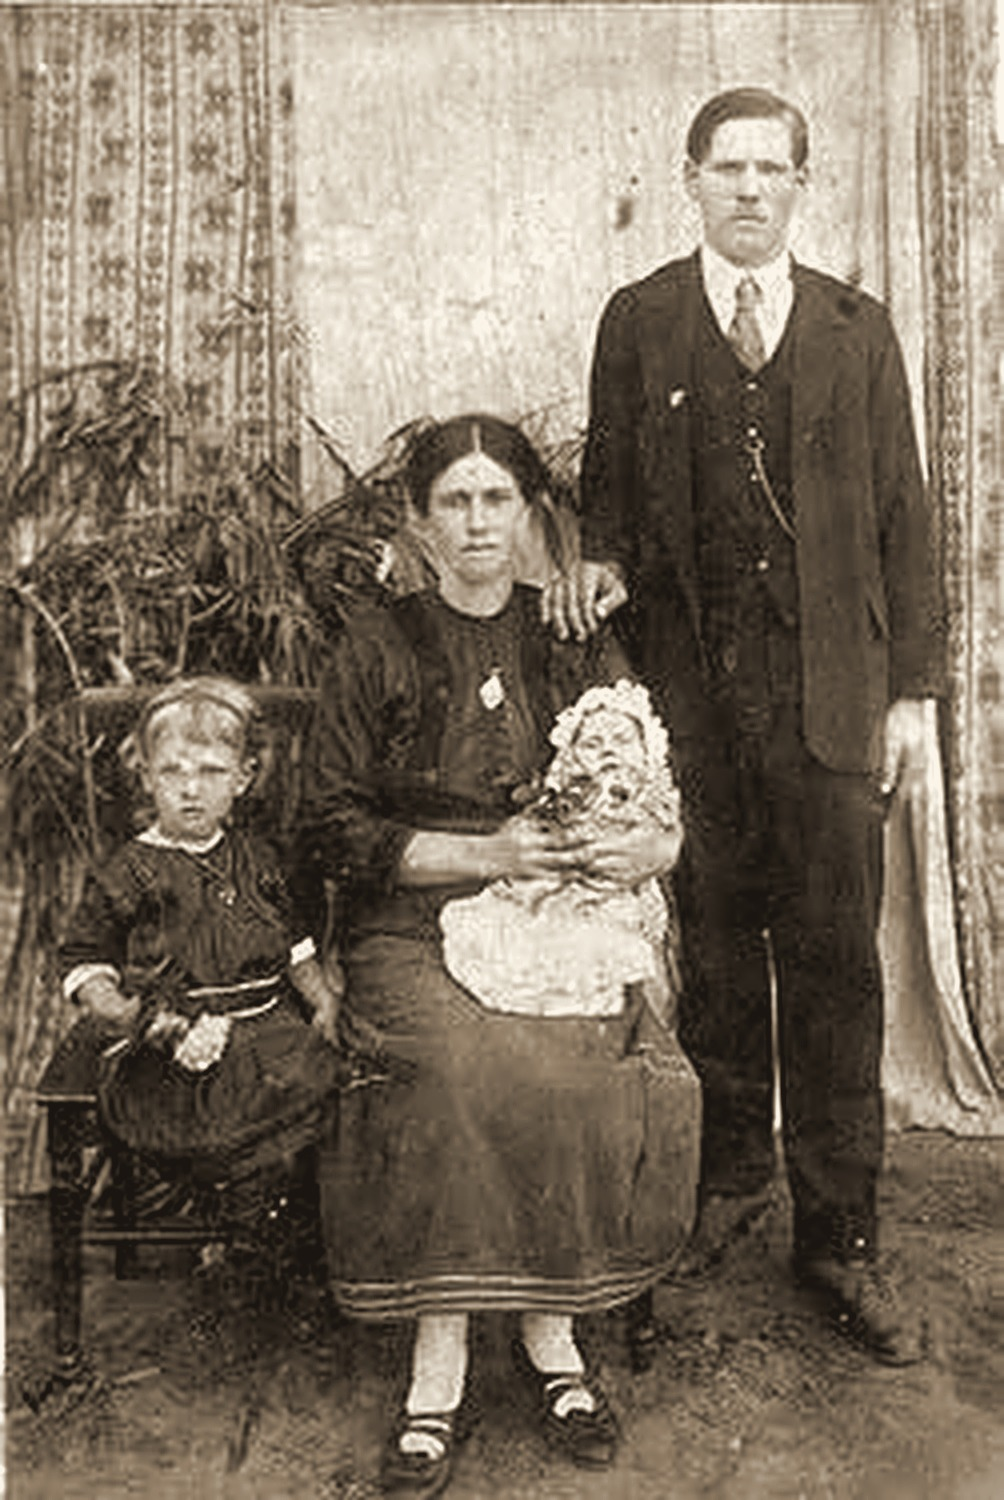
\includegraphics[width=0.6\linewidth,height=\textheight,keepaspectratio,alt={Fernando Dörner e Gertrudes Preiss com Hilda Ana, sentada na cadeira, e Adelina, a minha mãe, bebê no colo de Gertrudes. Por volta de 1927, pouco antes ou logo depois da mudança para Vidal Ramos. Reprodução de uma cópia pequena, ampliada e com contraste corrigido; o original está no repositório.}]{imagens/doerner_fernando_gertrudes_hilda_adelina_c1927_restaurada.jpg}
\caption{Fernando Dörner e Gertrudes Preiss com Hilda Ana, sentada na
cadeira, e Adelina, a minha mãe, bebê no colo de Gertrudes. Por volta de
1927, pouco antes ou logo depois da mudança para Vidal Ramos. Reprodução
de uma cópia pequena, ampliada e com contraste corrigido; o original
está no repositório.}
\end{figure}

É uma foto de estúdio do interior: uma cortina estampada, um vaso de
folhagens, uma cadeira para a menina. Fernando está de pé, de terno
escuro, colete e corrente de relógio, com a mão no ombro da mulher. Tem
uns trinta anos e o olhar sério de quem posa para um fotógrafo poucas
vezes na vida. Gertrudes, sentada, segura Adelina vestida de branco.
Hilda Ana, de vestido escuro, olha direto para a câmera. Quando a foto
circulou nas redes, em 2017, alguém da família escreveu que o bebê era o
tio Lindolfo; mas é a minha mãe, e o tio Lindolfo, então com uns dois
anos e meio, ficou fora do retrato. É o único rosto do meu avô que
conheço fora da memória. Para nós, os netos, ele era o \emph{Opapa}, e
Gertrudes, a \emph{Omama}. Se algum primo guarda outra fotografia de
Fernando Dörner, sobretudo dos anos de Vidal Ramos ou de Brusque, ela é
a peça que mais falta neste arquivo.

Do lado Haas, o Fata deixou marcas de fé visíveis: foi presbítero em
Ituporanga e construtor de igrejas. Fernando também era um homem muito
religioso. O artigo de 2011 conta que ele hospedou e alimentou os
construtores da igreja, do salão paroquial e da escola de Vidal Ramos,
abriu a Estrada da Igreja, doou terras para o Clube Esportivo Fluminense
e para a Escola Cacilda Guimarães e foi, por vários anos, delegado de
polícia, sem receber nada por isso. Diz também que era leitor assíduo e
assinante de revistas, que chegavam com dificuldade ao lugar. Não sei
ainda em que anos foi delegado, nem como isso se cruza com a história
que ele me contou.

Os pais de minha mãe não foram direto de São Martinho para Brusque.
Antes, viveram em Vidal Ramos, no Alto Vale, a cidade em que eu
cresceria. Foi lá que aconteceu essa história, que nenhum papel da
família registra.

Sempre gostei de ouvir histórias de gente mais velha, e isso não passou
despercebido à minha mãe. Quando eu já fazia o segundo grau, meu avô
veio morar na nossa casa. Estava com câncer de pele, a doença já
cheirava muito forte, e ele queria resolver os problemas dos terrenos
antes de morrer. Um dia, perguntei a ele como tinha sido a Segunda
Guerra em Vidal Ramos. Não perguntei o que ele tinha feito. Foi ele quem
sentiu que devia falar disso.

Meu avô me contou, então, que tinha apoiado Hitler e participado de
milícias de colonos que queriam apoiar uma invasão do Sul do Brasil pela
Alemanha. Contou também que mudou de lado. Segundo ele, foi lendo
revistas como as \emph{Seleções do Reader's Digest} que percebeu que
estava do lado errado. A mudança não foi aceita em Vidal Ramos. Junto
com as doenças de minha avó, foi uma das razões que o levaram a sair de
lá e ir para Brusque.

Disse que não passava um dia sem se arrepender de ter apoiado Hitler, e
que isso ele teria de resolver com Deus. Disse também que um líder como
Hitler exerce um encantamento sobre as pessoas, e que isso voltaria a
acontecer. Ele morreu em 1981. Não sei em quem pensava, nem se pensava
em alguém.

A palavra para o que ele foi naqueles anos é quinta-coluna: o morador de
um país disposto a ajudar, de dentro, a invasão de um exército de fora.
A palavra é minha, não dele, e a única prova que tenho é o que ele mesmo
me disse. Ele não precisava ter contado nada a um neto de quinze ou
dezesseis anos que nem tinha perguntado por isso. Contou assim mesmo,
doente e perto da morte.

Escrevo isso como guardei, sem acrescentar cenas e sem pôr aspas onde
não tenho as palavras exatas. Há um dado que ajuda a pôr a história no
tempo. A edição brasileira das \emph{Seleções do Reader's Digest}
começou a circular em fevereiro de 1942, o mês seguinte ao rompimento do
Brasil com a Alemanha, a Itália e o Japão, como parte da propaganda
americana da política da Boa Vizinhança. Se as revistas que ele leu eram
as \emph{Seleções} em português, a mudança de lado não pode ser anterior
a 1942. Não sei que grupo era esse, quem o organizava, quantos eram, se
tinham armas, nem em que anos ele participou. Não sei como as revistas
chegavam a Vidal Ramos, nem que artigos ele leu. A palavra ``milícia''
foi a que ele usou, ou a que eu guardei; pode ter sido uma organização
formal, ligada a algum partido ou associação, ou um grupo de vizinhos
que conversava e treinava. A história de Santa Catarina dos anos 1930 e
1940 tem de tudo isso, e não cabe a mim adivinhar qual era o caso dele.
Os historiadores que estudaram o período, como René Gertz e Marlene de
Fáveri, descrevem o quadro em que ele se moveu: o integralismo forte no
Vale do Itajaí até 1937; os núcleos do partido nazista entre os
teuto-brasileiros até a proibição de 1938; a campanha de nacionalização;
e, depois de 1942, o medo da ``quinta-coluna'', as buscas, as prisões e
as divisões dentro das próprias comunidades. Mostram também que não
existiu um plano militar alemão para invadir o Sul do Brasil, embora
muita gente nas colônias acreditasse nele, a favor ou contra. Nada disso
diz o que meu avô fez. Diz apenas que a história que ele me contou cabe
no seu tempo.

Também não foi o único conflito. Houve em Vidal Ramos uma disputa de
terras em que meu avô se colocou contra os outros colonos, e esses
colonos acabaram presos. O artigo de 2011 conta o episódio do mesmo
jeito, com mais detalhes. Muitos colonos se recusaram a pagar pelas
terras e se revoltaram contra a companhia que as tinha vendido.
Fernando, que tinha pago a sua, ficou do lado da companhia. Quando os
revoltosos foram presos em Brusque, foi ele quem fez roça para as
famílias que ficaram sem os homens, até que fossem soltos, cerca de um
ano depois, com a vitória da companhia. Ainda não sei o ano, o nome da
companhia nem os nomes dos presos.

O mesmo artigo lembra o outro lado da guerra. Na campanha do Estado Novo
contra os teuto-brasileiros, a família foi tratada como suspeita, e
falar e ler alemão virou agravante. O avô, ``decepcionado'', quase
proibiu os netos de aprender a língua, para protegê-los. O artigo não
fala de milícias. A memória pública da família guardou a perseguição; a
mim, ele contou também o que veio antes. As duas coisas podem ser
verdade.

Não sei a data, os nomes nem o lado da lei em cada momento da revolta
das terras. O que sei é que os dois episódios precisam ser lidos juntos,
dentro de uma história maior: os conflitos de terra nas colônias, a
desconfiança contra os teuto-brasileiros durante o Estado Novo e a
guerra, as prisões de colonos, as divisões dentro das próprias
comunidades. Um homem que mudou de lado numa questão e ficou contra os
vizinhos na outra não saiu de Vidal Ramos só por causa da saúde da
mulher.

Não vou julgar o meu avô com o que sei hoje, nem absolvê-lo com o que
não sei. Prefiro fazer o que um pesquisador faz quando um dado não
fecha: anotar, procurar a fonte e esperar. As perguntas para isso estão
listadas, uma a uma, num documento à parte do repositório. Elas vão a
jornais da época, a processos e inquéritos policiais, aos arquivos do
Estado e aos estudos sobre o nazismo e o integralismo em Santa Catarina.
Se as respostas vierem, entram aqui. Se não vierem, fica o que ele me
contou. Para quem ouviu, isso também é uma fonte: a de um homem que, já
velho e doente, disse ao neto que tinha errado, que tinha mudado e que
se arrependia todos os dias.

\section{Dois óbitos em Brusque}\label{dois-uxf3bitos-em-brusque}

\emph{Brusque, Santa Catarina, abril de 1970 e maio de 1981}

Os dois últimos documentos deste capítulo são certidões de óbito, e as
leio com o cuidado que se tem com uma carta de família.

Gertrudes morreu primeiro. Foi às oito e meia da noite de 9 de abril de
1970, em casa, em Brusque. O médico, Dr.~Germano Hoffmann, atestou
carcinoma. O termo foi lavrado no cartório de registro civil em 14 de
abril, e quem compareceu para declarar a morte foi o próprio marido,
Fernando Doerner, que assina ao pé do termo. A certidão diz que ela era
natural de Imaruí, tinha setenta e quatro anos, era doméstica, filha de
Manoel Preus e de Helena Michels, ambos falecidos, e casada com Fernando
Doerner, com quem deixava seis filhos maiores. O escrivão os escreveu em
sequência: Hilda Ana, Lindolfo, Adelina, Irma, Olga e Lino Fernando. A
sepultura foi feita no cemitério católico da cidade.

\begin{figure}
\centering
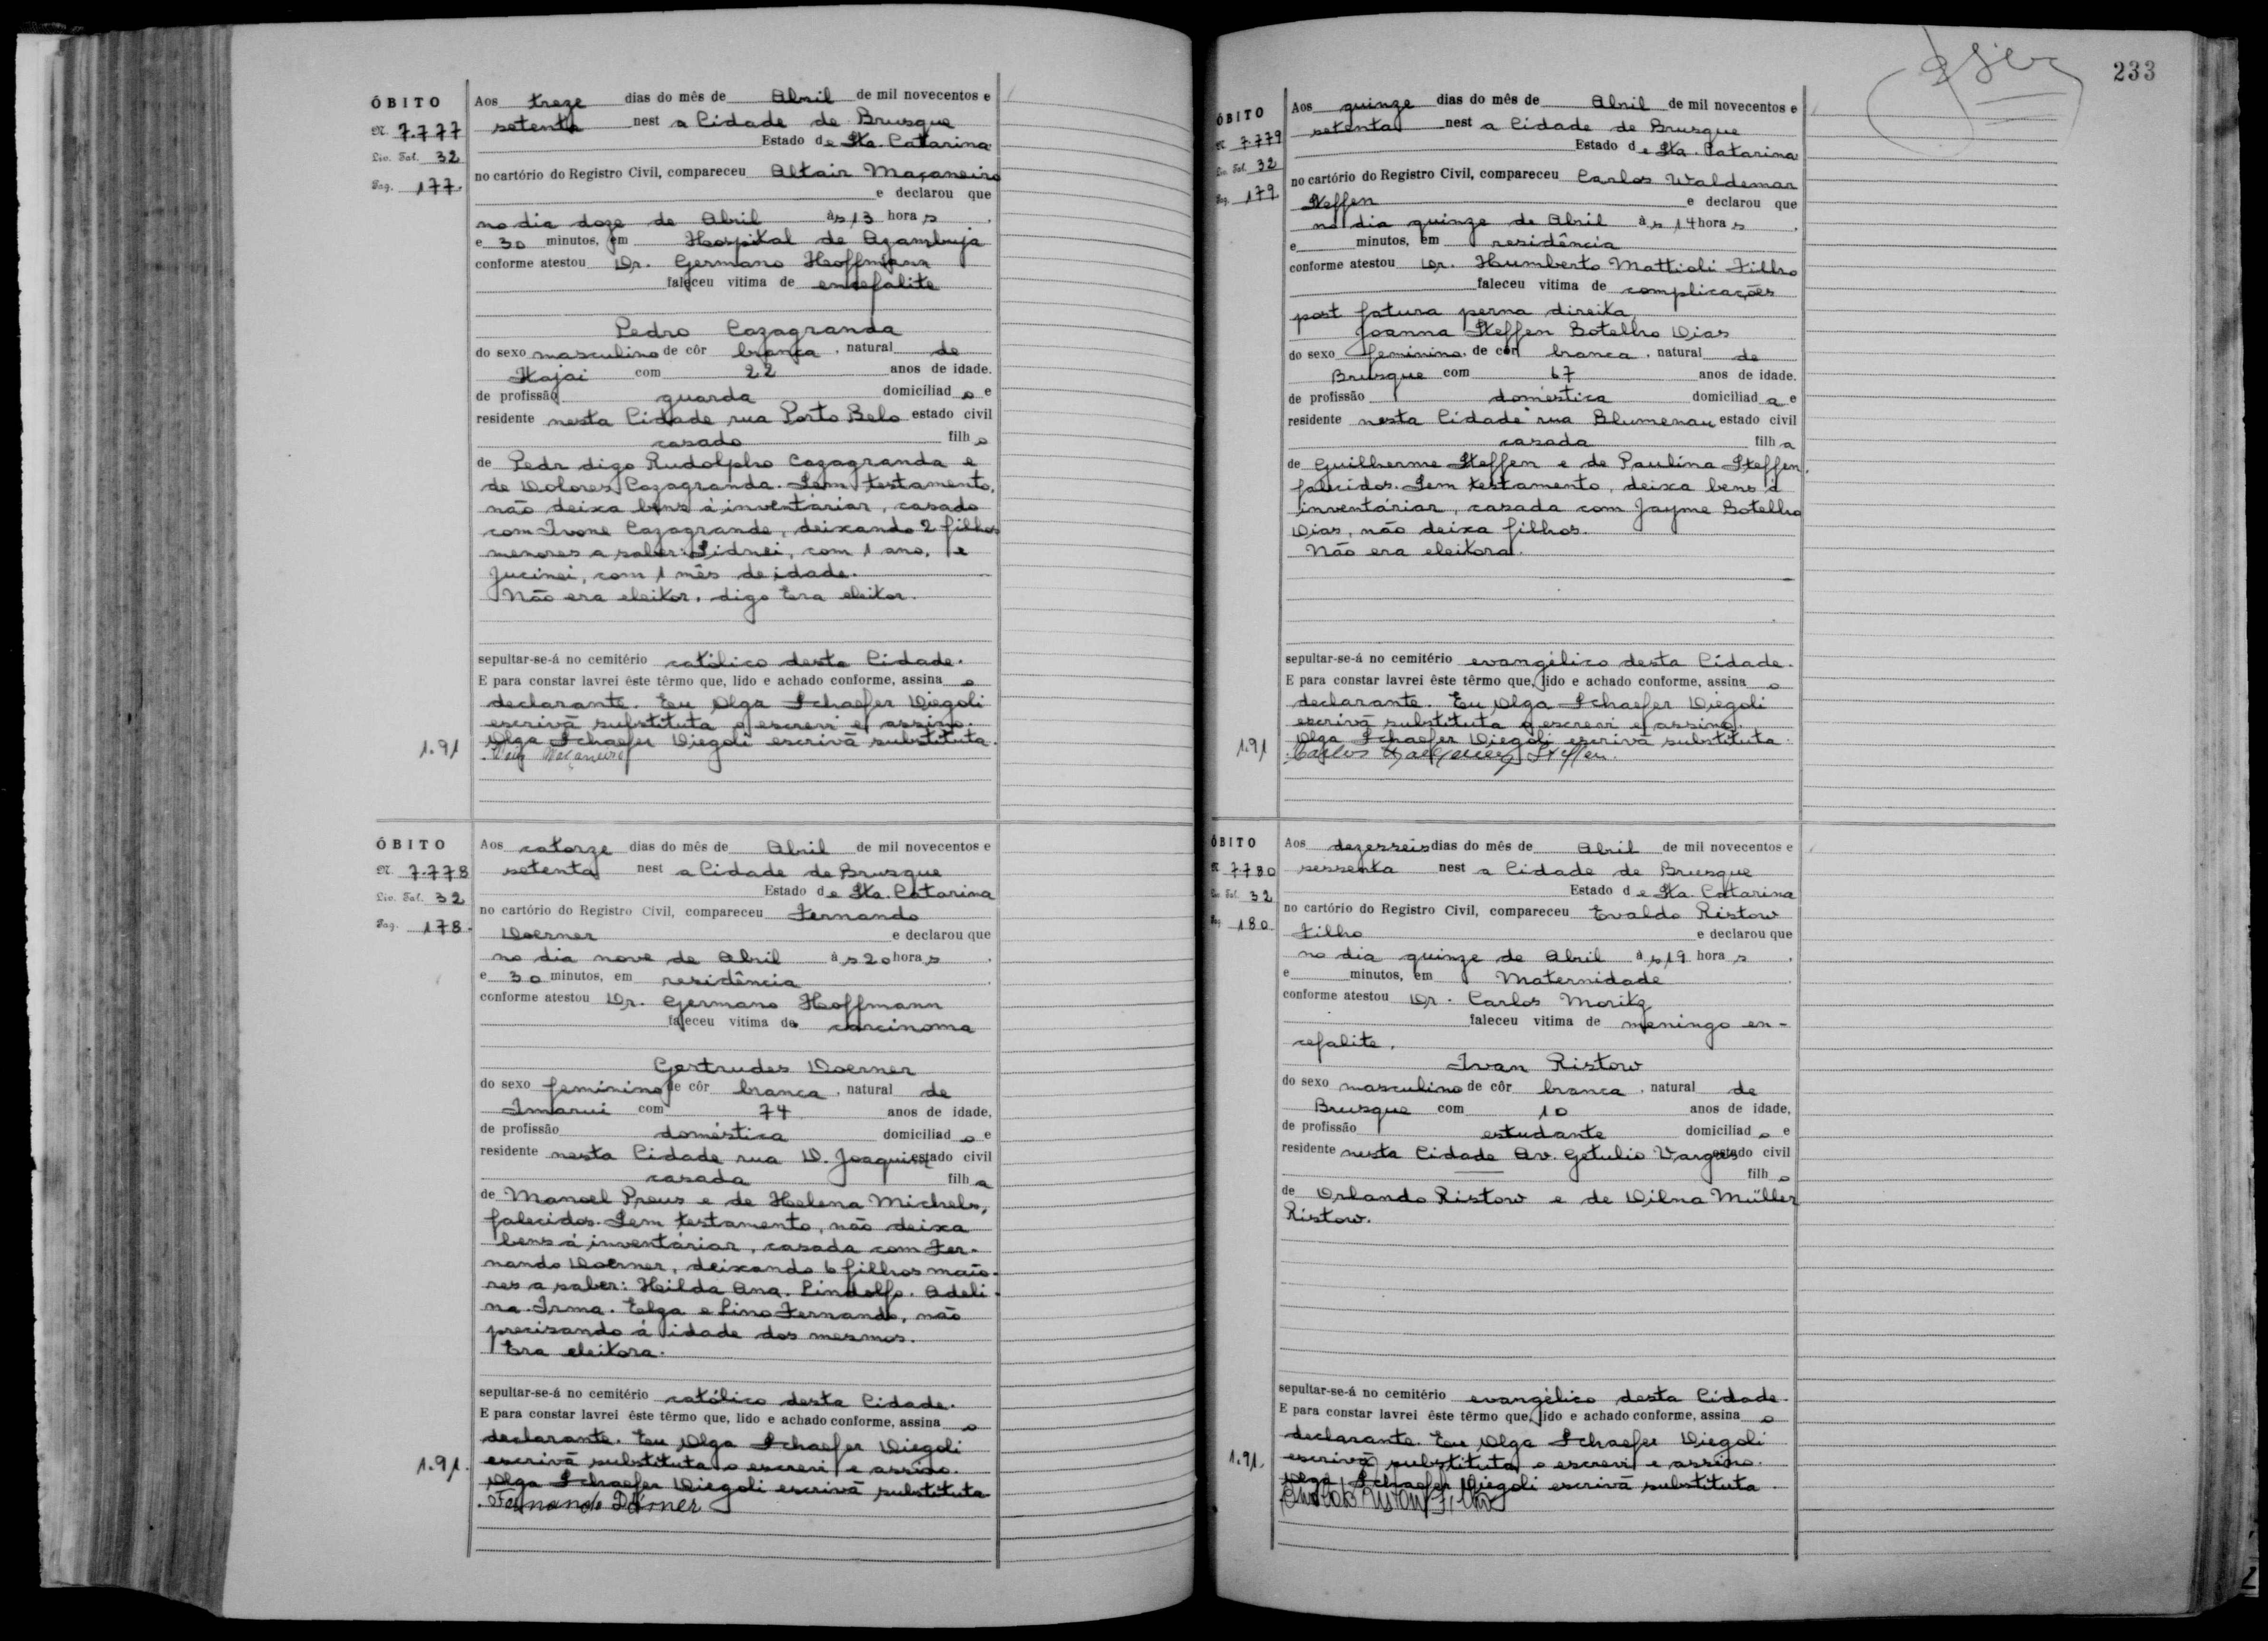
\includegraphics[width=0.85\linewidth,height=\textheight,keepaspectratio,alt={Livro de óbitos do Registro Civil de Brusque, abril de 1970: o termo de Gertrudes Doerner (canto inferior esquerdo), natural de Imaruí, 74 anos, filha de Manoel Preus e Helena Michels, casada com Fernando Doerner, que é o declarante e assina o registro.}]{imagens/doc_doerner_obito_gertrudes_preiss_1970.jpg}
\caption{Livro de óbitos do Registro Civil de Brusque, abril de 1970: o
termo de Gertrudes Doerner (canto inferior esquerdo), natural de Imaruí,
74 anos, filha de Manoel Preus e Helena Michels, casada com Fernando
Doerner, que é o declarante e assina o registro.}
\end{figure}

Há um detalhe que me comove mais que os outros. O declarante é o marido.
Em quase todos os óbitos que li nesta pesquisa, quem vai ao cartório é
um filho, um genro, um vizinho, às vezes um funcionário da funerária.
Aqui foi Fernando, aos setenta e dois anos, quem ditou ao escrivão o
nome dos sogros e dos seis filhos e assinou. Não sei se fez isso por
costume, por dever ou porque não quis deixar que outro fizesse. A
assinatura está lá, no pé do termo 7.778, folha 178 do livro 32.

Fernando viveu mais onze anos. Morreu às dez da manhã de 21 de maio de
1981, em casa, em Brusque, ``sem assistência médica'', como diz o termo.
Não houve atestado de médico, e por isso o termo não dá a causa. Eu o
tinha visto, pouco antes, doente de câncer de pele, em nossa casa; não
sei quando voltou para Brusque. Tinha oitenta e três anos. Era
aposentado, natural de Imaruí, viúvo, filho de Carlos Dörner e de Anna
Eller, ambos falecidos. Deixava cinco filhos maiores, sem testamento e
sem bens a inventariar, o que talvez queira dizer que os terrenos
estavam resolvidos, e era eleitor. Foi sepultado no Cemitério Municipal
da cidade, que a família conhece como Parque da Saudade.

\begin{figure}
\centering
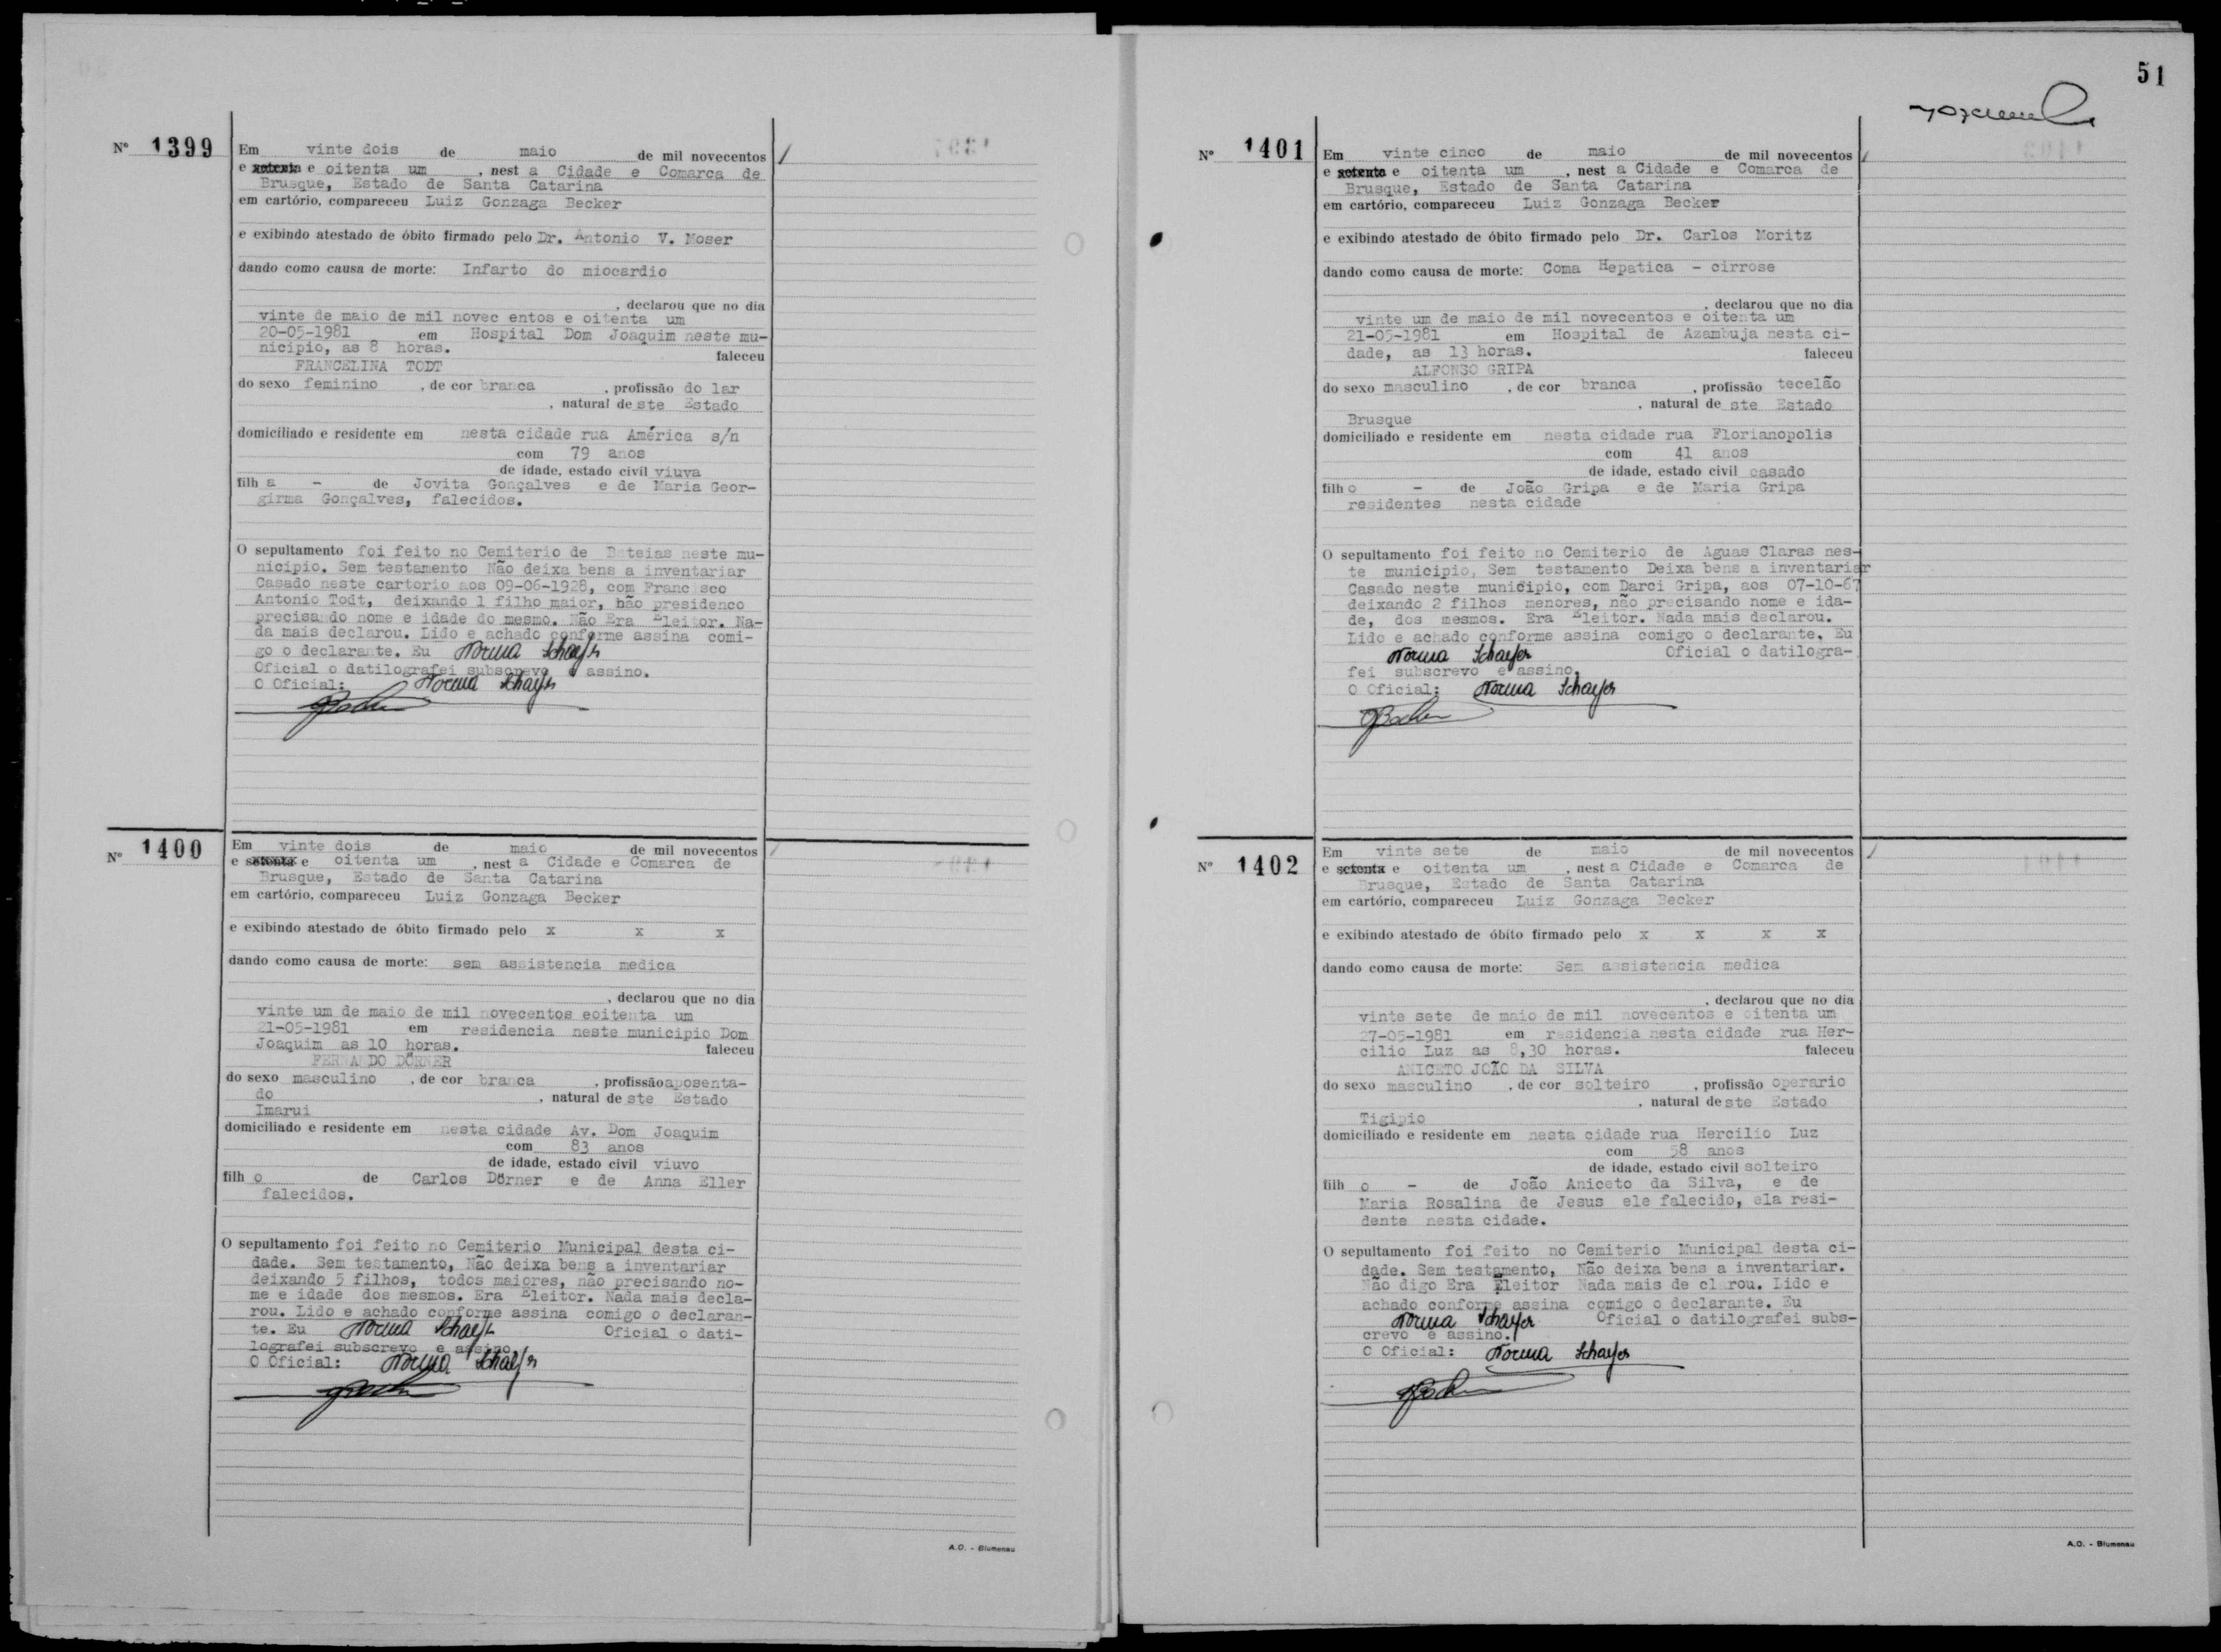
\includegraphics[width=0.85\linewidth,height=\textheight,keepaspectratio,alt={Livro de óbitos do Registro Civil de Brusque, maio de 1981: o termo nº 1400 (canto inferior esquerdo), de Fernando Dörner, 83 anos, aposentado, natural de Imaruí, viúvo, filho de Carlos Dörner e Anna Eller.}]{imagens/doc_doerner_obito_fernando_1981.jpg}
\caption{Livro de óbitos do Registro Civil de Brusque, maio de 1981: o
termo nº 1400 (canto inferior esquerdo), de Fernando Dörner, 83 anos,
aposentado, natural de Imaruí, viúvo, filho de Carlos Dörner e Anna
Eller.}
\end{figure}

\begin{ficha}

\textbf{Ficha do Arquivo}: (1) Óbito de Gertrudes Doerner, Registro
Civil de Brusque, livro 32, fl.~178, termo nº 7.778, lavrado em
14/04/1970; falecimento em 09/04/1970, às 20h30, na residência; atestado
do Dr.~Germano Hoffmann, carcinoma; natural de Imaruí, 74 anos; filha de
Manoel Preus e Helena Michels; declarante: Fernando Doerner; seis filhos
maiores: Hilda Ana, Lindolfo, Adelina, Irma, Olga e Lino Fernando;
sepultura no cemitério católico de Brusque. (2) Óbito de Fernando
Dörner, Registro Civil de Brusque, termo nº 1400, lavrado em 22/05/1981;
falecimento em 21/05/1981, às 10h, na residência, ``sem assistência
médica''; natural de Imaruí, 83 anos, aposentado, viúvo; filho de Carlos
Dörner e Anna Eller; cinco filhos maiores; sepultura no Cemitério
Municipal. Arquivos:
\texttt{imagens/doc\_doerner\_obito\_gertrudes\_preiss\_1970.jpg} e
\texttt{imagens/doc\_doerner\_obito\_fernando\_1981.jpg}.

\end{ficha}

Duas observações de investigador. A primeira: os dois documentos dizem
``natural de Imaruí'', e não São Martinho, como o FamilySearch. Não há
contradição, porque quando eles nasceram São Martinho pertencia a
Imaruí, e o escrivão de Brusque escreveu o nome do município de então.
Um detalhe desses parece pequeno, mas quem procura registros de batismo
nos livros errados perde meses por causa dele. A segunda: em 1970 havia
seis filhos vivos, e em 1981 eram cinco. Entre um termo e outro, um dos
filhos de Fernando e Gertrudes morreu. As duas certidões não dizem qual,
mas o registro civil de Brusque diz: Lino Fernando, o caçula dos que
sobreviveram, morreu em 14 de fevereiro de 1979, aos quarenta e um anos.
Fernando enterrou um filho dois anos antes de morrer.

Brusque é uma cidade de rio. Nasceu em 1860 como Colônia Itajahy, na
margem do Itajaí-Mirim, o braço menor do grande rio que atravessa o
Vale. A água foi, como em todas as colônias, estrada, energia e risco.
Movimentou as primeiras tecelagens que deram à cidade a sua fama e, de
tempos em tempos, subiu para dentro das casas. Fernando morreu em maio
de 1981. Três anos depois, em agosto de 1984, uma das grandes cheias do
Vale do Itajaí inundou Brusque. Vieram outras em novembro de 2008, no
desastre que matou cerca de cento e trinta e cinco pessoas em Santa
Catarina, e em 2011. Em todas houve a mesma combinação de chuva
persistente vinda do mar contra a encosta da serra, um rio estreito
encaixado entre morros e uma cidade construída onde a água sempre
passou. Eu trabalho com modelos de cheias no Itajaí, e quando abro o
mapa de áreas inundáveis de Brusque procuro, quase sem querer, a rua
onde moravam os meus avós. Não vou escrever aqui o nome dela. Basta
dizer que, se tivessem vivido um pouco mais, teriam visto o rio entrar
na cidade como entrou no Vale inteiro. No Capítulo 13 volto a esses
rios, que no fim são um só problema.

Penso às vezes na distância entre o primeiro e o último documento deste
capítulo. De um lado, a Renânia das forjas, onde nasce um menino por
volta de 1854. Do outro, um cartório de Brusque em 1981, onde o filho
dele, já velho, é registrado como ``aposentado'' e ``eleitor'', duas
palavras que nenhum Dörner de Solingen teria imaginado ao lado do
próprio nome. O caminho entre esses dois pontos passa pela Vestfália dos
Eller, por dez filhos de uma mulher que morreu cedo, por uma capela no
Capivari onde dois cristãos de confissões talvez diferentes precisaram
de uma dispensa para casar, por mais cinco filhos de outra mãe, por um
caçula que nunca conheceu a dele e por uma moça que descendia dos barcos
de 1828. Desse caminho saiu Adelina, e de Adelina saí eu.

Com este capítulo fecho a parte paterna da árvore de vocês. Do lado do
meu pai e da minha mãe, já tínhamos quatro séculos de história. Faltava
a outra metade dos meus filhos.

\section{Para vocês descobrirem}\label{para-vocuxeas-descobrirem-9}

\begin{itemize}
\tightlist
\item
  Qual dos noivos de 1900 não era católico? Procurem a página do ato de
  Hulda em São Ludgero, de 28 de abril de 1900, que só conheço pelo
  índice, e a outra via do assento nº 23.
\item
  Em que ano e em que navio Carlos Dörner embarcou, e ele nasceu mesmo
  em Solingen? Nenhum documento que tenho responde.
\item
  Que grupo era esse de que meu avô Fernando participou, quem o
  organizava e em que anos? As perguntas estão num documento à parte do
  repositório e vão a jornais da época, a processos e inquéritos
  policiais e aos arquivos do Estado.
\item
  Quando meu avô disse que o encantamento por um líder como Hitler
  voltaria a acontecer, de que estava falando? Olhem o tempo de vocês e
  decidam se ele acertou.
\item
  Algum primo guarda outra fotografia de Fernando Dörner, sobretudo dos
  anos de Vidal Ramos ou de Brusque? Perguntem também aos parentes de
  Vidal Ramos o que se conta sobre a revolta das terras: o ano, a
  companhia, os presos.
\end{itemize}

\part{Os Horizontes de Bárbara}\label{os-horizontes-de-buxe1rbara}

\begin{boletim}

Ar úmido subindo o Vale do Taquari. Correntes contínuas entre Joinville,
Estrela e Arroio do Meio. Microclimas de família.

\end{boletim}

\chapter{Na Garagem da Oma Rosita, nos Retratos do Vô Erno e no Legado
do Dr.~Carlos Heinz Funke}\label{cap-11}

\begin{quote}
\emph{Há casas onde o Natal começa pelo cheiro das bolachas. Foi numa
delas que a outra metade desta história me esperava.}
\end{quote}

\emph{26,3° S · 48,8° O, Joinville, SC}

\section{Quatro gerações numa
garagem}\label{quatro-gerauxe7uxf5es-numa-garagem}

Na fotografia que abre este capítulo há cinco pessoas, e a legenda da
família só dá nome a quatro. A imagem é a fotografia de uma fotografia.
Alguém fotografou com o celular uma página de álbum e, sem querer,
deixou na parte de cima da imagem um pedaço da página anterior: um
beiral branco, um céu muito azul e dois pássaros escuros pousados na
calha. Embaixo, protegida pelo plástico do álbum, está a cena que
importa. É uma garagem em Joinville, no início de 2005. Atrás, uma porta
de madeira e um carro escuro, e lá fora o verde de um quintal.

Segundo a legenda que a família escreveu para ela, estão ali quatro
gerações. A bisavó Oma Rosita Lohmann Hoeveler, de cabelos brancos e
vestido florido, apoiada num andador de alumínio. A neta dela, Bárbara,
de vestido estampado, com a barriga redonda de quem espera o segundo
filho. Esse filho é você, Lucas, que nasceria em 10 de março daquele
ano. E a avó, a Dra. Ilusca Leocádia Hoeveler Funke, com um menino loiro
de camiseta azul no colo: você, Matheus, que tinha nascido em 20 de
junho de 2002. Por uma coincidência que nunca deixa de me divertir, você
nasceu no mesmo dia do meu aniversário. Recebi um presente com trinta e
sete anos de atraso.

\begin{figure}
\centering
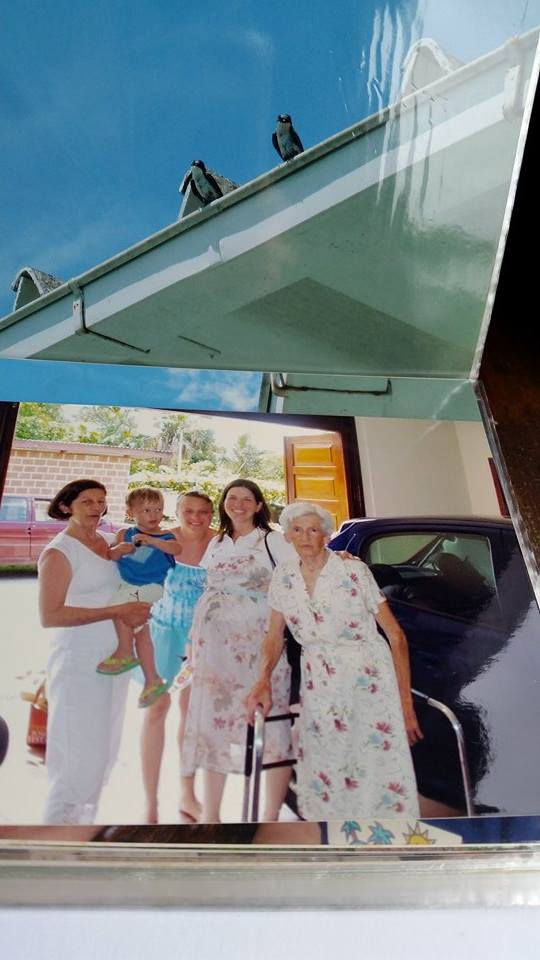
\includegraphics[width=0.85\linewidth,height=\textheight,keepaspectratio,alt={Quatro gerações na garagem da casa da família em Joinville, no início de 2005: a bisavó Oma Rosita Lohmann Hoeveler, com o andador; Bárbara Funke Haas, grávida de Lucas; e a avó Dra. Ilusca Leocádia Hoeveler Funke com Matheus no colo. A imagem é uma reprodução de uma página de álbum.}]{imagens/lohmann_4_geracoes_oma_rosita_ilusca_barbara_matheus.jpg}
\caption{Quatro gerações na garagem da casa da família em Joinville, no
início de 2005: a bisavó Oma Rosita Lohmann Hoeveler, com o andador;
Bárbara Funke Haas, grávida de Lucas; e a avó Dra. Ilusca Leocádia
Hoeveler Funke com Matheus no colo. A imagem é uma reprodução de uma
página de álbum.}
\end{figure}

Gosto dessa imagem pelo que ela mostra e pelo que ela esconde. Mostra
uma linha de mulheres: Rosita, que nasceu em 1918 no Vale do Taquari, no
Rio Grande do Sul; Ilusca, que cresceu entre Estrela e Nova Petrópolis;
Bárbara, que nasceu em Joinville em 27 de julho de 1972. Esconde quase
tudo o que veio antes delas: os veleiros de 1846, uma fazenda de vinte e
quatro colônias, uma mulher morta vinte e seis dias depois de um parto,
uma casa nova em Palmas, diante do Salto do Taquari. Nada disso aparece
na fotografia, mas tudo isso estava ali dentro, de pé numa garagem, num
dia de verão. A quinta pessoa, uma moça de vestido azul, a legenda não
identifica, e eu a deixo assim.

Nos capítulos anteriores segui as correntes que desembocam em mim: os
Haas e os Meier da Baviera, os Doerner, os Preiss, os Michels e os Arns.
Agora preciso fazer o que um meteorologista faz quando percebe que a sua
retrotrajetória só explicou metade da umidade de uma tempestade:
procurar a outra fonte. Matheus e Lucas não são só Haas. São também
Funke, Hoeveler, Lohmann, Endres, Schnack e Wingert. Essa metade eu não
posso contar sozinho.

Por isso, nesta Parte IV, Bárbara fala também. Os trechos em itálico,
introduzidos sempre com o nome dela, são dela, na primeira pessoa. O
resto continua sendo a minha voz, a de quem chegou a essa família de
fora, como genro, e foi aprendendo os nomes aos poucos.

\section{A outra metade}\label{a-outra-metade}

Joinville tem um clima que eu, como meteorologista, sempre achei
teatral. A cidade fica espremida entre a Baía da Babitonga, a leste, e a
muralha da Serra do Mar, a oeste, ali chamada de Serra Dona Francisca. O
ar úmido que vem do oceano é empurrado contra a encosta, sobe, esfria e
despeja a umidade em forma de chuva. Por isso chove tanto em Joinville.
É uma das cidades mais chuvosas do Sul do Brasil, com dias inteiros de
garoa e tardes de verão em que a chuva cai pesada sem nenhum aviso. Os
colonos que chegaram em 1851 para fundar a Colônia Dona Francisca
aprenderam isso logo. Os descendentes deles guardam até hoje o hábito de
ter um guarda-chuva perto da porta.

Foi nessa cidade, entre o mar e a serra, que os Funke se estabeleceram,
e foi para ela que vieram, mais tarde, os Hoeveler do Rio Grande do Sul.
O pai de Bárbara, o médico Carlos Heinz Funke, nasceu ali em 10 de
agosto de 1939. A mãe, Ilusca, chegou do Rio Grande. Não sei, e não vou
inventar, onde e como os dois se conheceram. Ele se formou em Medicina
no Rio Grande do Sul, e a vida acadêmica em Porto Alegre ou nos
arredores é o cenário mais provável, mas é só uma hipótese. Sei que se
casaram, que tiveram quatro filhos (Bárbara, Katherine, Alessandra e
Paulo Jacques) e que Oma Rosita passou os últimos anos perto deles, em
Joinville.

Os Funke trazem uma surpresa que eu só vi quando juntei as duas árvores.
Nos registros do FamilySearch, Paulo Funke e Hulda, os bisavós de
Bárbara, nasceram em Glauchau, na Saxônia, em 1881 e 1889, e o filho
deles, Oscar Martin, avô de Bárbara, nasceu no distrito de Glauchau em
1º de dezembro de 1910. Glauchau fica a poucas dezenas de quilômetros de
Chemnitz. E Chemnitz é a cidade onde a minha família lembra que o Fata e
a Mota moravam antes de partir, em 1913. Por volta de 1910, portanto, é
possível que os bisavós do meu lado e os de Bárbara vivessem na mesma
região da Saxônia, sem saber uns dos outros, e que todos tenham acabado
em Santa Catarina. Nenhum papel diz que se cruzaram. E há mais um galho
longe dali: Dora Marta, a Oma Dora, era filha de Jacques Aenishaenslin,
nascido na Suíça, numa família de Ormalingen, perto de Basileia.

Quando casei com Bárbara, juntei à minha árvore um galho que eu não
conhecia. Do meu lado, católicos da Baviera e do Mosela, com uma
dispensa de religião mista perdida no Capivari, como vocês viram no
capítulo anterior. Do lado dela, luteranos de Braunschweig, de
Schleswig-Holstein, da tradição evangélica do Vale do Taquari e da Serra
Gaúcha. Do meu lado, gente que construía igrejas com as mãos. Do lado
dela, gente que ensinava e curava. Não quero transformar isso em
fórmula, porque as famílias são mais misturadas do que qualquer resumo,
mas o contraste existe e eu o senti desde os primeiros almoços de
domingo em Joinville.

Aqui passo a palavra a Bárbara.

\emph{Na minha lembrança, a Oma Rosita faz parte da casa de Joinville
tanto quanto a cozinha. Ela vinha do Rio Grande, de uma família de doze
irmãos, e eu demorei muito para entender o que isso queria dizer. Quando
ela falava dos irmãos, os nomes pareciam de personagens: Urbano,
Armando, Sunta, Arlindo. Por muito tempo, para mim, foram mais nomes do
que rostos: gente que vivia longe, num vale de onde ela tinha saído
havia muito tempo.}

\emph{O nome que me liga a ela mais diretamente nem é o meu, é o da
minha mãe. Ilusca Leocádia. O Leocádia veio da bisavó, Miguelina
Leocádia Endres, a mãe da Oma Rosita. Na nossa família os nomes passam
assim, por dentro, no segundo nome, como uma coisa que não se anuncia
mas também não se perde.}

\section{O médico de Pirabeiraba}\label{o-muxe9dico-de-pirabeiraba}

O Dr.~Carlos Heinz Funke, que aparece nos documentos ora como Heinz, ora
como Heins, morreu em Joinville em 1989, por volta dos cinquenta anos.
Bárbara era adolescente. Eu não o conheci. Sei dele o que a família
conta e o que a cidade guardou, e a cidade guardou bastante.

Em Pirabeiraba, o distrito rural ao norte de Joinville, ao pé da serra,
duas instituições públicas levam o nome dele. Uma é a Unidade Básica de
Saúde da Família Dr.~Carlos Heinz Funke. A outra é a Escola Agrícola
Municipal Carlos Heins Funke, criada em 1989, o ano da morte dele, e
autorizada a funcionar em 15 de fevereiro de 1990.

\begin{ficha}

\textbf{Ficha do Arquivo}: Escola Agrícola Municipal Carlos Heins Funke,
Pirabeiraba, Joinville (SC). Criada em 1989 pelo Decreto nº 6168/89 e
pelo Parecer 452/89; funcionamento autorizado em 15/02/1990; APP
reconhecida de utilidade pública pela Lei nº 3.968, de 05/07/1999.
Oferece o ensino fundamental (6º ao 9º ano) com pré-qualificação em
agropecuária, em período integral, para alunos de todo o município.
Fonte: página institucional da APP da escola (consulta em 2026).

\end{ficha}

Gosto de imaginar o que esse nome numa escola agrícola diria a um homem
que passou a vida entre consultórios e hospitais. A página da escola
explica que o objetivo é preparar o jovem para atuar na propriedade
rural da família, ``despertando o interesse pela permanência no campo''.
É quase uma resposta, cem anos depois, ao drama de todas as famílias
deste livro, que tinham filhos demais para a terra que havia e os viam
partir. Não sei se o Dr.~Carlos Heinz pensou nisso alguma vez. Sei que
os nomes que uma cidade dá às suas escolas e postos de saúde são uma
forma de dizer quem cuidou dela.

Da família dele tenho duas fotografias, e as duas pedem cuidado na
leitura.

A primeira é um retrato de estúdio em sépia, manchado pelo tempo, que a
família guarda como ``o bisavô e a família de Oma Dora''. Oma Dora é a
mãe do Dr.~Carlos Heinz, a avó paterna de Bárbara. No centro, sentados,
um homem de bigode, terno claro e colete, e uma mulher de vestido branco
de gola larga, com as mãos no colo. Em volta deles, nove jovens: rapazes
de gravata, moças de cabelo curto à moda do fim dos anos 1920, uma
menina de franja reta, um menino de colarinho aberto. Se a minha
contagem está certa, são nove filhos. A identificação de cada rosto,
inclusive o de Dora, ainda está por confirmar com quem a conhece, e eu
não vou arriscar.

\begin{figure}
\centering
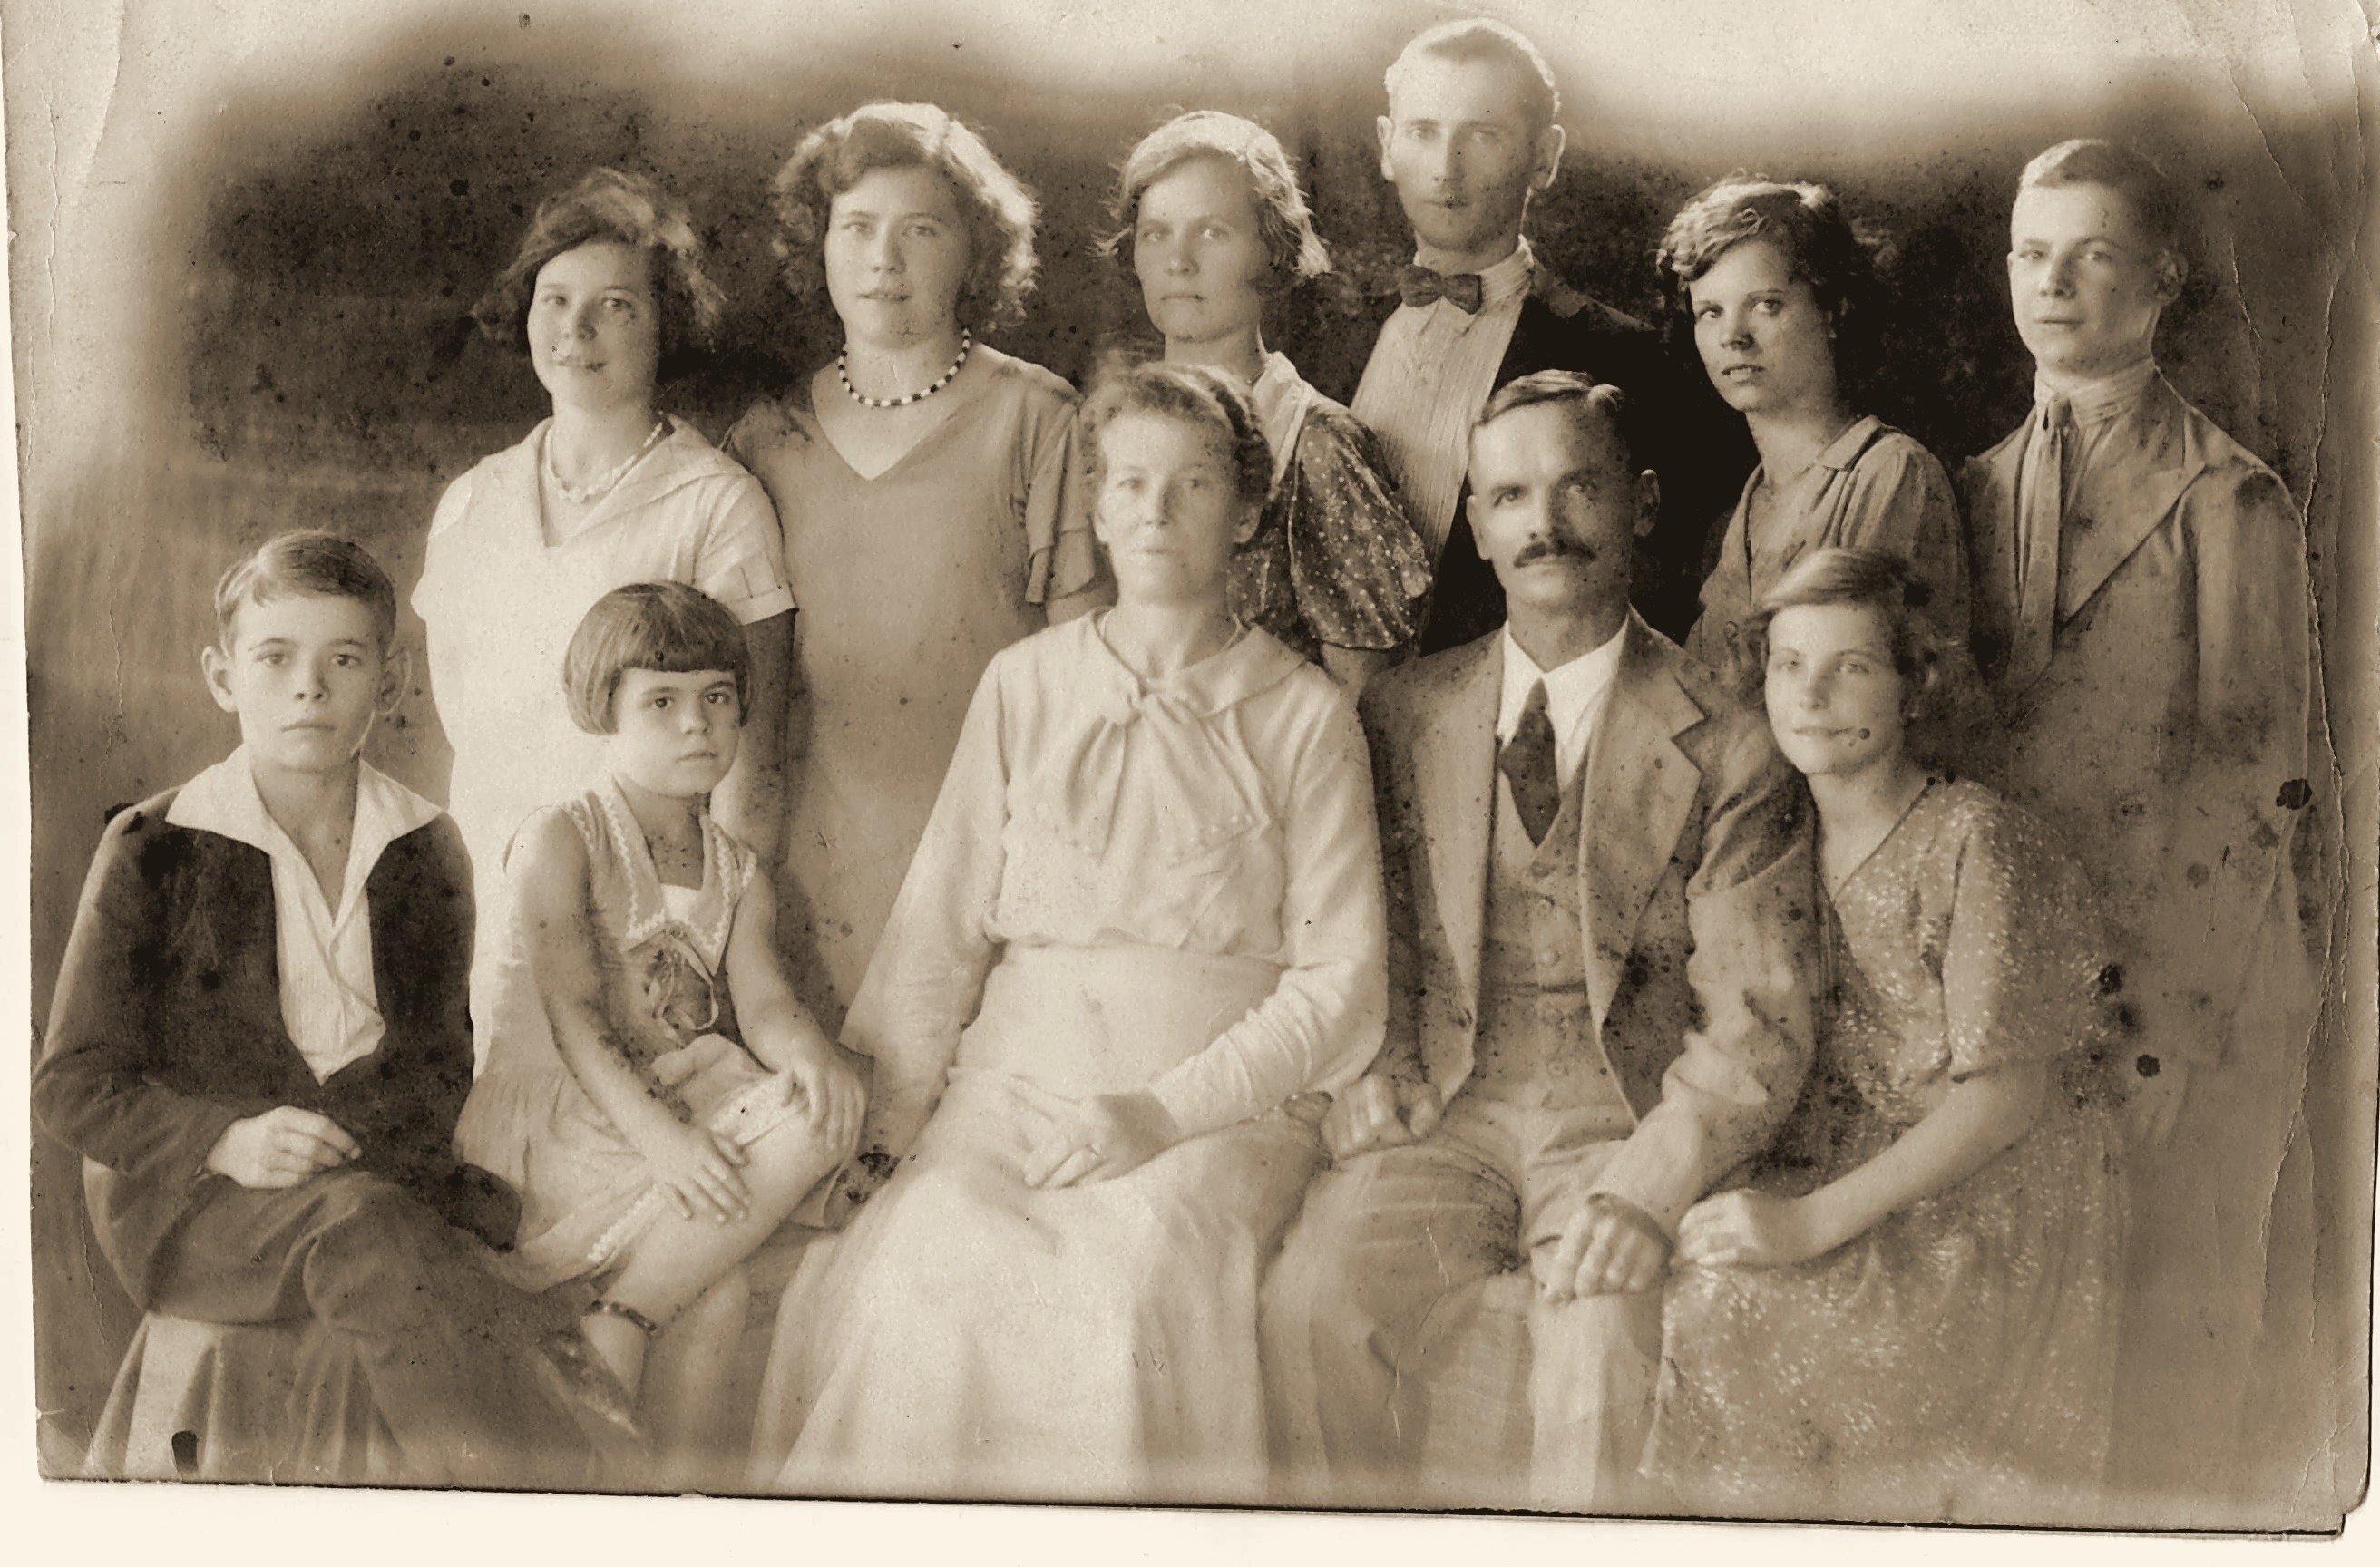
\includegraphics[width=0.85\linewidth,height=\textheight,keepaspectratio,alt={Retrato de família em sépia, guardado como ``o bisavô e a família de Oma Dora'': o casal sentado ao centro, cercado pelos filhos, provavelmente no fim da década de 1920 ou início da de 1930. A identificação individual está por confirmar. Contraste e tons corrigidos.}]{imagens/funke_bisavo_e_familia_oma_dora_restaurada.jpg}
\caption{Retrato de família em sépia, guardado como ``o bisavô e a
família de Oma Dora'': o casal sentado ao centro, cercado pelos filhos,
provavelmente no fim da década de 1920 ou início da de 1930. A
identificação individual está por confirmar. Contraste e tons
corrigidos.}
\end{figure}

A segunda foi tirada cinquenta e poucos anos depois, num salão de festas
com lustres de cristal e cortinas vermelhas. Na toalha de uma mesa
enfeitada de margaridas brancas, alguém escreveu à caneta a data:
22/01/83. Oito pessoas posam lado a lado e riem: seis mulheres de
vestidos estampados e dois homens de terno, um deles de cravo branco na
lapela. A família registra a imagem como ``Oma Dora com seus sete
irmãos''. Oito, portanto, é a soma certa, Dora e mais sete. Se no
retrato antigo havia nove filhos, um dos irmãos não chegou à festa de
1983, ou a minha contagem do retrato antigo está errada. Prefiro deixar
a pergunta para Bárbara e as irmãs dela a forçar uma resposta.

\begin{figure}
\centering
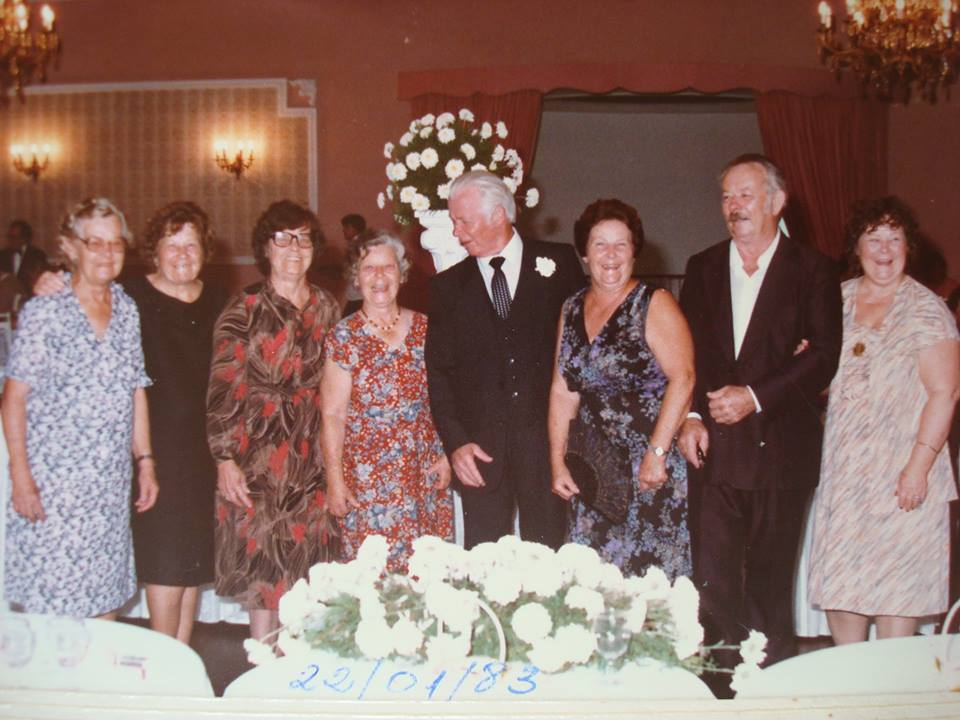
\includegraphics[width=0.85\linewidth,height=\textheight,keepaspectratio,alt={Oma Dora e seus sete irmãos num salão de festas, em 22 de janeiro de 1983 (data escrita na toalha da mesa).}]{imagens/funke_oma_dora_7_irmaos_1983.jpg}
\caption{Oma Dora e seus sete irmãos num salão de festas, em 22 de
janeiro de 1983 (data escrita na toalha da mesa).}
\end{figure}

Olhando as duas imagens juntas, vejo uma coisa que a genealogia
raramente consegue mostrar: o tempo agindo sobre as mesmas pessoas. Os
jovens sérios do estúdio, que olham para a câmera com a solenidade de
quem não sabe se haverá outra fotografia, viram os velhos risonhos do
salão, que já não têm medo da câmera e se abraçam para caber no quadro.
Entre uma imagem e outra cabem uma guerra mundial, a Campanha de
Nacionalização, que proibiu o alemão nas escolas e nas ruas, e a
transformação de Joinville de cidade colonial em cidade industrial. Cabe
também a vida inteira do Dr.~Carlos Heinz, que em janeiro de 1983 tinha
quarenta e três anos e mais seis pela frente.

Pirabeiraba, onde estão a escola e o posto que levam o nome dele, é um
bom lugar para entender Joinville. O distrito fica ao norte da cidade,
onde a planície encontra a serra. Por ali passa a velha Estrada Dona
Francisca, aberta no século XIX para ligar a colônia do litoral ao
planalto de São Bento, uma das obras de que os colonos mais se
orgulhavam. É uma terra de sítios, de bananais e arrozais, de casas de
colonos com jardins cuidados, e também de rios que descem da serra com
pressa e transbordam com facilidade depois de uma chuva forte. Um médico
que trabalhasse ali atendia agricultores, operários que desciam todos os
dias para as fábricas da cidade, crianças com verminose, velhos com
pressão alta. Não tenho a lista dos lugares onde o Dr.~Carlos Heinz
atendeu, e não vou inventá-la. Mas a escolha do nome dele para duas
instituições daquele distrito diz, com bastante clareza, que foi ali que
a cidade o reconheceu.

Sobre o pai, Bárbara escreve pouco, e eu respeito a medida.

\emph{É estranho ver o nome do próprio pai numa placa. A gente cresce
chamando de pai uma pessoa que, para os outros, era o doutor. Depois que
ele morreu (eu era adolescente), o nome dele foi para uma escola e para
um posto de saúde, e deixou de ser só nosso. Hoje acho que isso é uma
forma de herança também: saber que o trabalho de alguém continuou
servindo depois que ele se foi, em lugares onde nenhum de nós estava.}

\section{O professor de Nova
Petrópolis}\label{o-professor-de-nova-petruxf3polis}

Do lado da mãe de Bárbara, a fotografia mais antiga que tenho é de uma
escola. Também ela é uma reprodução: uma foto pequena, em preto e
branco, posta sobre um tecido cor-de-rosa e fotografada de cima. Nela,
umas quatro dezenas de alunos estão alinhados em fileiras diante de um
prédio, os da frente agachados, os de trás de pé, quase todos de camisa
ou blusa branca e as meninas de saia escura. No centro, de terno escuro,
um homem adulto. Atrás, o que parece ser uma bandeira. É o Vô Erno
Hoeveler, bisavô de vocês, professor.

\begin{figure}
\centering
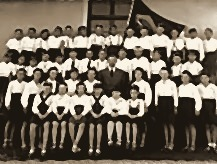
\includegraphics[width=0.85\linewidth,height=\textheight,keepaspectratio,alt={O bisavô Erno Hoeveler (``Vô Erno''), professor luterano em escolas comunitárias do Rio Grande do Sul, cercado por seus alunos. Reprodução de uma fotografia antiga. Contraste e tons corrigidos.}]{imagens/hoeveler_vo_erno_escola_restaurada.jpg}
\caption{O bisavô Erno Hoeveler (``Vô Erno''), professor luterano em
escolas comunitárias do Rio Grande do Sul, cercado por seus alunos.
Reprodução de uma fotografia antiga. Contraste e tons corrigidos.}
\end{figure}

Erno Hoeveler foi professor em escolas da comunidade evangélica em
Estrela e em Nova Petrópolis, no Rio Grande do Sul. Casou com Rosita
Érica Lohmann, a filha de Francisco Jacob Lohmann e Miguelina Endres, e
teve com ela quatro filhos, entre eles Ilusca e Walter. Nas colônias
alemãs do Sul, o professor da escola comunitária era uma figura central,
muitas vezes o único homem letrado da localidade além do pastor.
Ensinava a ler em alemão e em português, ensinava aritmética e o
catecismo, e com frequência regia o coral e ajudava no culto. Não era um
ofício que enriquecesse ninguém. A própria Ilusca disse isso com toda a
simplicidade numa reportagem de jornal sobre os Natais de antigamente em
Joinville: o pai era professor e ganhava pouco, e por isso muitos
presentes de Natal eram consertados e reaproveitados, e às vezes o
presente eram maçãs e biscoitos.

Na mesma reportagem, ela conta dois presentes que marcaram a infância.
Uma boneca, que guarda até hoje, já com os olhos afundados pelo tempo, e
um violino usado que o pai comprou numa casa de penhores em Porto
Alegre. Leio essa frase e vejo o Vô Erno, que eu também não conheci,
entrando numa casa de penhores da capital com o salário curto de
professor de colônia, escolhendo entre objetos que outras famílias
tinham deixado por necessidade e saindo com um violino para a filha. Não
sei o ano nem a loja, e não preciso saber. Quando Ilusca casou, contou
ela, deu o violino a um sobrinho.

Ilusca, a filha do professor que ganhava pouco, tornou-se advogada. Para
uma moça nascida por volta de 1943 numa família de colônia, filha de um
professor de escola comunitária, isso foi um salto de geração tão grande
quanto o de Johann Haas ao trocar a Baviera por Rio do Ouro. Em duas
gerações, a família que vivia do salário curto de um mestre-escola
passou a ter, numa mesma casa de Joinville, uma advogada e um médico.
Não romantizo esse salto. Imagino que ele tenha custado anos de estudo,
distância de casa e alguma solidão, como custou a todos os filhos de
colonos que foram os primeiros da família a entrar numa faculdade. Mas
ele aconteceu, e foi feito com a mesma matéria-prima que o violino da
casa de penhores: a convicção de que valia a pena gastar com o que forma
uma pessoa.

A tradição de ensinar parece correr fundo nesse lado da família. No
Capítulo 12 vocês vão ler que o primeiro Lohmann a chegar ao Rio Grande
do Sul, em 1846, era filho de professor, e que a liga dos Lohmann da
Alemanha se orgulhava de ter tido mestres-escolas e pastores ``em todas
as ramificações'' desde o século XVII. Erno era Hoeveler, não Lohmann, e
casou com a família, não nasceu nela. Mesmo assim, é difícil não ver ali
um padrão. Os Lohmann tinham uma tradição de professores e casaram uma
filha com um professor.

A fé luterana era o outro fio. Aqui Bárbara fala de novo.

\emph{A Kathe contou isso a um jornal de Joinville melhor do que eu
contaria: o Natal chegava quando a Oma começava a fazer bolachas. As
forminhas, a minha mãe disse na mesma entrevista, ainda são as mesmas. O
Advento era levado a sério, com a coroa de quatro velas, uma acesa a
cada domingo, e os hinos cantados pelo hinário. Na noite de 24, a minha
mãe entrava primeiro na sala e acendia as velas, e os outros entravam
depois, cantando. No presépio, o berço ficava vazio até o dia de Natal,
porque o Menino Jesus só chegava quando nascia.}

\emph{Quando o meu pai morreu, alguém precisou ficar no lugar dele na
noite de Natal, puxando as reflexões e os cantos. Foi o nosso irmão, o
pianista da família. Penso que essa é uma herança tão concreta quanto
uma casa: o lugar à frente da família na noite de 24, que passa de um
para outro quando alguém falta.}

Para o investigador que há em mim, o valor desse trecho é que ele não
depende só da memória de uma pessoa. A reportagem publicada em Joinville
traz os depoimentos de Katherine e de Ilusca, e as duas descrevem a
mesma casa e os mesmos ritos. A Oma das bolachas, as velas do Advento e
o berço vazio estão documentados.

De Nova Petrópolis veio também o tio que deu nome a um livro. Walter
Hoeveler, irmão de Ilusca, o Tio Walter da família, mudou-se para
Florianópolis em 1960. Katherine Funke, jornalista e escritora, irmã de
Bárbara, publicou em 2013 \emph{Viagens de Walter}, inspirado nele.
Gosto de pensar que nesta família, além de ensinar, também se escreve.
Katherine escreveu sobre o tio, Bárbara escreve aqui comigo, e eu
escrevo para vocês.

\section{A caixa de retratos}\label{a-caixa-de-retratos}

Oma Rosita morreu em Joinville em 2014, com noventa e poucos anos. A
reportagem sobre os Natais saiu um ano depois, e nela a família conta
que, no primeiro Natal sem ela, o pinheirinho de verdade foi trocado por
um artificial, com pisca-pisca. Ilusca explicou a troca com uma conta
simples: antes eram seis pessoas para montar a árvore, e agora era só
ela. Em toda a reportagem, é a frase que mais me toca: fala de mão de
obra. É assim que as perdas aparecem numa família: alguém falta, e uma
tarefa que era de muitos passa a ser de um só.

Depois da morte de Rosita ficaram as coisas dela, entre elas os
retratos. Não sei se estavam todos numa caixa, como se diz nas
histórias, ou espalhados em álbuns e gavetas. Sei que entre eles havia
um que, para esta investigação, valia mais que todos os outros.

É um retrato de casamento numa moldura de papelão cor de terra, com uma
barra decorada em linhas finas. Não é oval, como eu me lembrava e como
cheguei a escrever no rascunho do roteiro deste livro: a memória
arredonda as coisas. A noiva está à esquerda, com um véu longo preso por
uma coroa de flores, vestido branco de gola alta e mangas compridas, e o
rosto sério e redondo. O noivo está à direita, de terno escuro com
colete, gravata-borboleta branca, um raminho de flores na lapela e uma
corrente de relógio aparecendo no colete. Tem bigode, cabelo curto
penteado para o lado e a mão da noiva apoiada no braço. Atrás deles, o
cenário pintado de um estúdio de fotógrafo, com uma janela falsa e uma
folhagem desenhada. São Francisco Jacob Lohmann e Miguelina Leocádia
Endres, no casamento de 5 de setembro de 1914. Bisavós de Bárbara.
Trisavós de vocês.

\begin{figure}
\centering
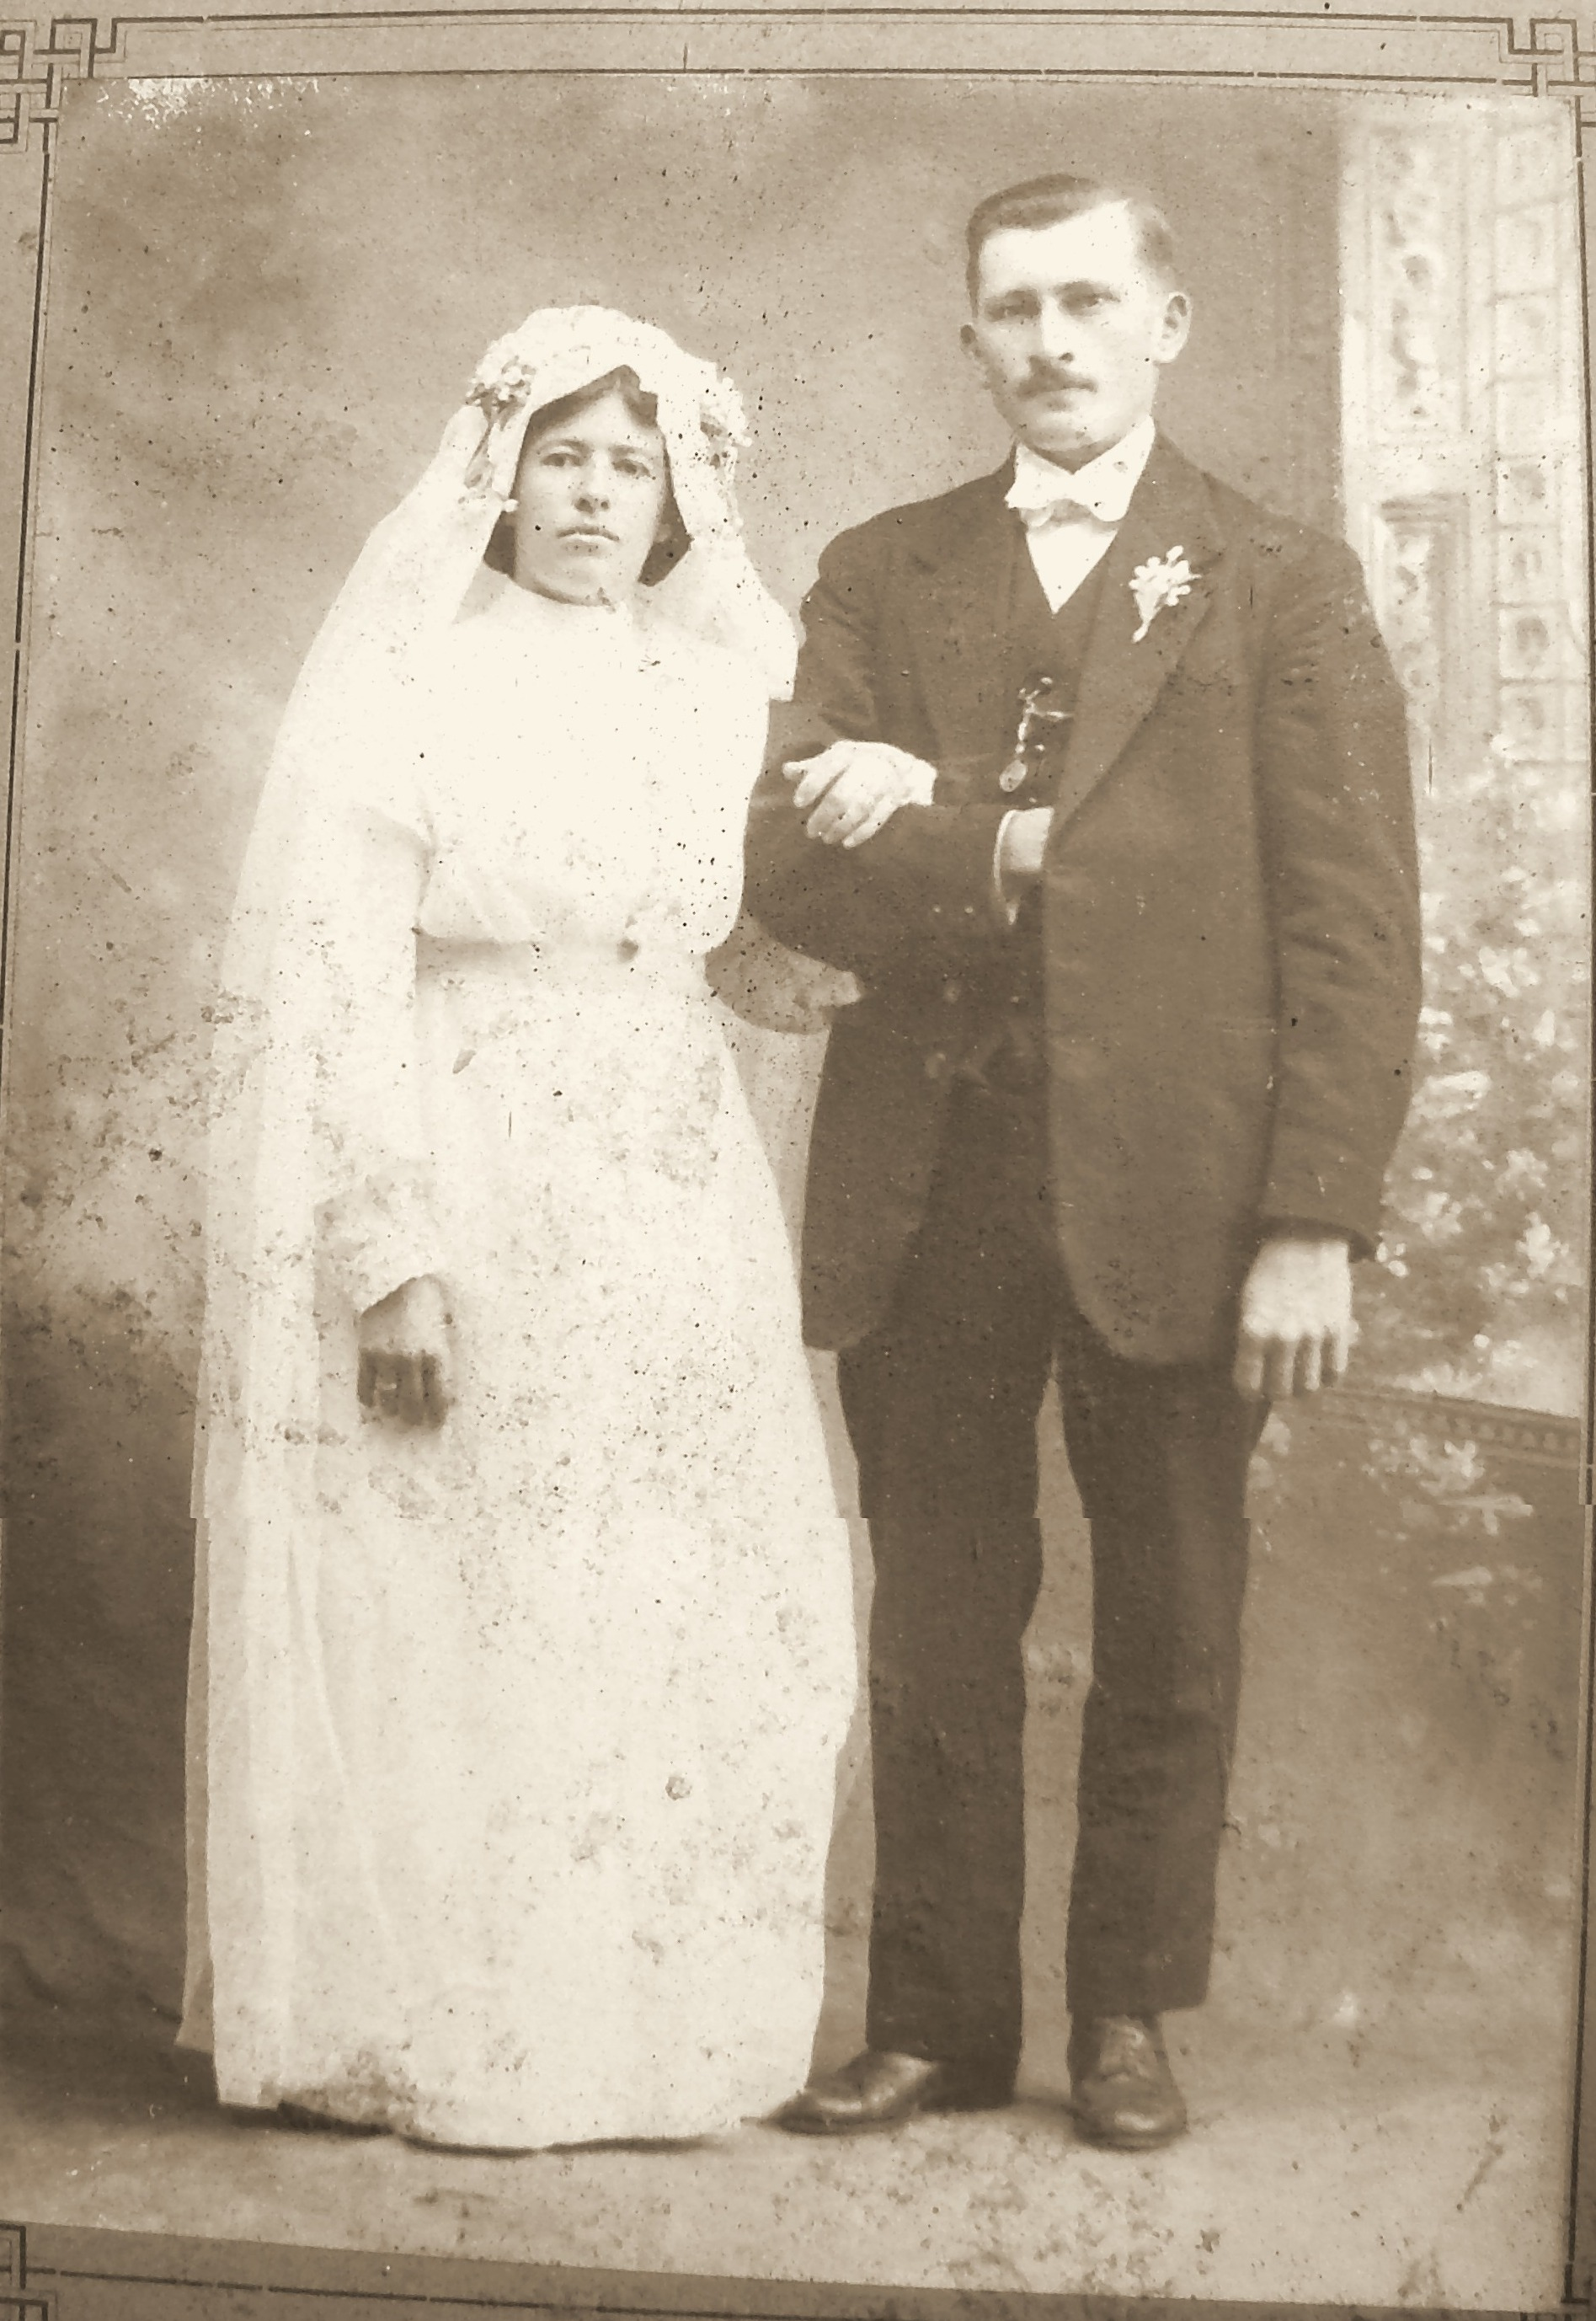
\includegraphics[width=0.85\linewidth,height=\textheight,keepaspectratio,alt={Retrato de casamento de Francisco Jacob Lohmann (1889--1975) e Miguelina Leocádia Endres (n.~1891), de 5 de setembro de 1914, guardado por Oma Rosita: os bisavós de Bárbara e trisavós de Matheus e Lucas. Contraste e tons corrigidos.}]{imagens/lohmann_bisavo_francisco_e_bisavo_michelina_restaurada.jpg}
\caption{Retrato de casamento de Francisco Jacob Lohmann (1889--1975) e
Miguelina Leocádia Endres (n.~1891), de 5 de setembro de 1914, guardado
por Oma Rosita: os bisavós de Bárbara e trisavós de Matheus e Lucas.
Contraste e tons corrigidos.}
\end{figure}

Faço a conta, por hábito. Francisco nasceu em 20 de novembro de 1889,
portanto tinha vinte e quatro anos no dia do retrato. Miguelina, nascida
em 9 de dezembro de 1891, tinha vinte e dois. Do outro lado do oceano,
um mês antes, tinha começado a Primeira Guerra Mundial. Em Santa
Catarina, os Haas estavam fazia um ano e meio no Brasil e tinham
enterrado Luisa e Walter. Nada disso aparece no retrato, e talvez nada
disso tenha chegado àquele estúdio do Vale do Taquari, onde um rapaz que
nunca conheceu a mãe posava, de bigode e gravata-borboleta, para começar
a própria família.

Esse rapaz que nunca conheceu a mãe é a pista que me levou ao capítulo
seguinte. Quando montei a árvore no FamilySearch, a ficha de Francisco
Jacob trouxe uma data que me fez parar: a mãe dele, Suzana Regina
Schnack, morreu em 16 de dezembro de 1889, vinte e seis dias depois de
ele nascer. Esse homem cresceu sem mãe e teria, com a moça de véu do
retrato, doze filhos. Uma das filhas foi Rosita, que guardou o retrato a
vida inteira e o deixou para a neta.

Fecho este capítulo com Bárbara.

\emph{Eu já tinha visto esse retrato muitas vezes sem olhar para ele de
verdade. Era a foto dos bisavós, e pronto. Só quando o Reinaldo começou
a montar a árvore, e a gente se sentou com as datas na frente, foi que
eu entendi que o rapaz de bigode tinha perdido a mãe com menos de um mês
de vida. Fiquei pensando na mulher que o criou, na casa onde ele cresceu
e no que quer dizer, para um homem assim, ter doze filhos. Não sei se a
Oma Rosita conhecia essa história em detalhe. Se conhecia, talvez
achasse que não era coisa de contar.}

\emph{Foi aí que decidimos ir. Se a Oma não estava mais lá para contar,
os irmãos dela ainda estavam. Em setembro de 2012 fomos com os meninos
para o Rio Grande.}

Na ordem do livro, conto essa viagem agora, depois da morte de Rosita.
Na ordem da vida, ela aconteceu antes, em setembro de 2012, quando Oma
Rosita ainda estava viva em Joinville e quatro dos irmãos dela nos
esperavam no Vale do Taquari. Para entender quem eram Francisco e
Miguelina no retrato de casamento, precisávamos descer a serra até lá.

\section{Para vocês descobrirem}\label{para-vocuxeas-descobrirem-10}

\begin{itemize}
\tightlist
\item
  Quando e por que os Funke vieram de Glauchau para Joinville? Os Funke
  e os Haas chegaram a se cruzar na Saxônia antes de 1913?
\item
  Quem é a moça de vestido azul da fotografia da garagem? Perguntem à
  mãe de vocês e às tias.
\item
  No retrato antigo da família de Oma Dora contei nove filhos; na festa
  de 22 de janeiro de 1983 estão Dora e mais sete. Um dos irmãos faltou,
  ou contei errado? Bárbara e as irmãs dela são as primeiras a quem
  perguntar.
\item
  Onde e como Carlos Heinz Funke e Ilusca se conheceram? A vida
  acadêmica em Porto Alegre é só uma hipótese minha.
\item
  Quem é o sobrinho que ganhou o violino da casa de penhores quando
  Ilusca casou, e onde está esse violino hoje?
\end{itemize}

\chapter{Da Fazenda Lohmann aos Cemitérios de Estrela --- O Vale do
Taquari}\label{cap-12}

\begin{quote}
\emph{Os rios do Sul têm memória longa. Quem mora na beira deles também
precisa ter.}
\end{quote}

\emph{29,3° S · 51,9° O, Palmas, Arroio do Meio, RS}

A família diz que Francisco Jacob Lohmann e Miguelina Leocádia Endres
tiveram doze filhos. Os registros dão a dois deles datas de nascimento
anteriores ao casamento dos pais e trazem dois Walter. Na fotografia da
casa nova, contei onze.

\section{Setembro de 2012}\label{setembro-de-2012}

\emph{Arroio do Meio e Estrela, Rio Grande do Sul, 25 de setembro de
2012}

Chegamos ao Vale do Taquari na primavera, com os morros muito verdes e o
rio largo correndo entre eles. Matheus tinha dez anos e Lucas tinha
sete. Levávamos uma lista de nomes. O objetivo da viagem era simples de
dizer e difícil de cumprir: encontrar, enquanto ainda estavam vivos, os
irmãos de Oma Rosita.

Dos doze filhos de Francisco Jacob Lohmann e Miguelina Leocádia Endres,
alguns ainda viviam em 2012, espalhados por Arroio do Meio, Estrela e
arredores, em casas de colônia e de cidade pequena. Pelas datas que o
FamilySearch nos dá, o Tio Urbano tinha cerca de noventa e oito anos, o
Tio Armando, cerca de noventa e seis, a Tia Sunta, cerca de noventa e
um, e o caçula, o Tio Arlindo, oitenta e oito. Eram a última geração que
tinha visto Francisco e Miguelina com os próprios olhos.

Não vou reconstituir aqui as conversas daqueles dias. Não as gravei como
gravei a minha mãe nas Bodas, e a memória que tenho delas é a de um
visitante emocionado, não a de um escrivão. Seria fácil pôr na boca dos
tios frases bonitas sobre a enchente de 1941, sobre o pai viúvo, sobre a
casa nova. Não farei isso. O que posso fazer é descrever as fotografias,
que não mentem sobre o que mostram, e dizer o que senti.

A visita ao Tio Armando foi numa varanda de colônia. Na fotografia, ele
está sentado numa cadeira baixa, de suéter escuro de lã, com os cabelos
brancos desalinhados e um sorriso torto de quem acha graça de alguma
coisa que ficou fora do quadro. Estou sentado ao lado dele, de jaqueta,
com o braço passado pelos ombros dele. A legenda da família diz que
Bárbara estava comigo nessa visita. Atrás, uma coluna de alvenaria
descascada, uma antena parabólica velha, um galpão de tijolos, o pasto e
o morro coberto de mata. O céu está branco. É a paisagem de quase todas
as colônias alemãs do Sul, e eu a reconheci como se fosse a de Vidal
Ramos.

\begin{figure}
\centering
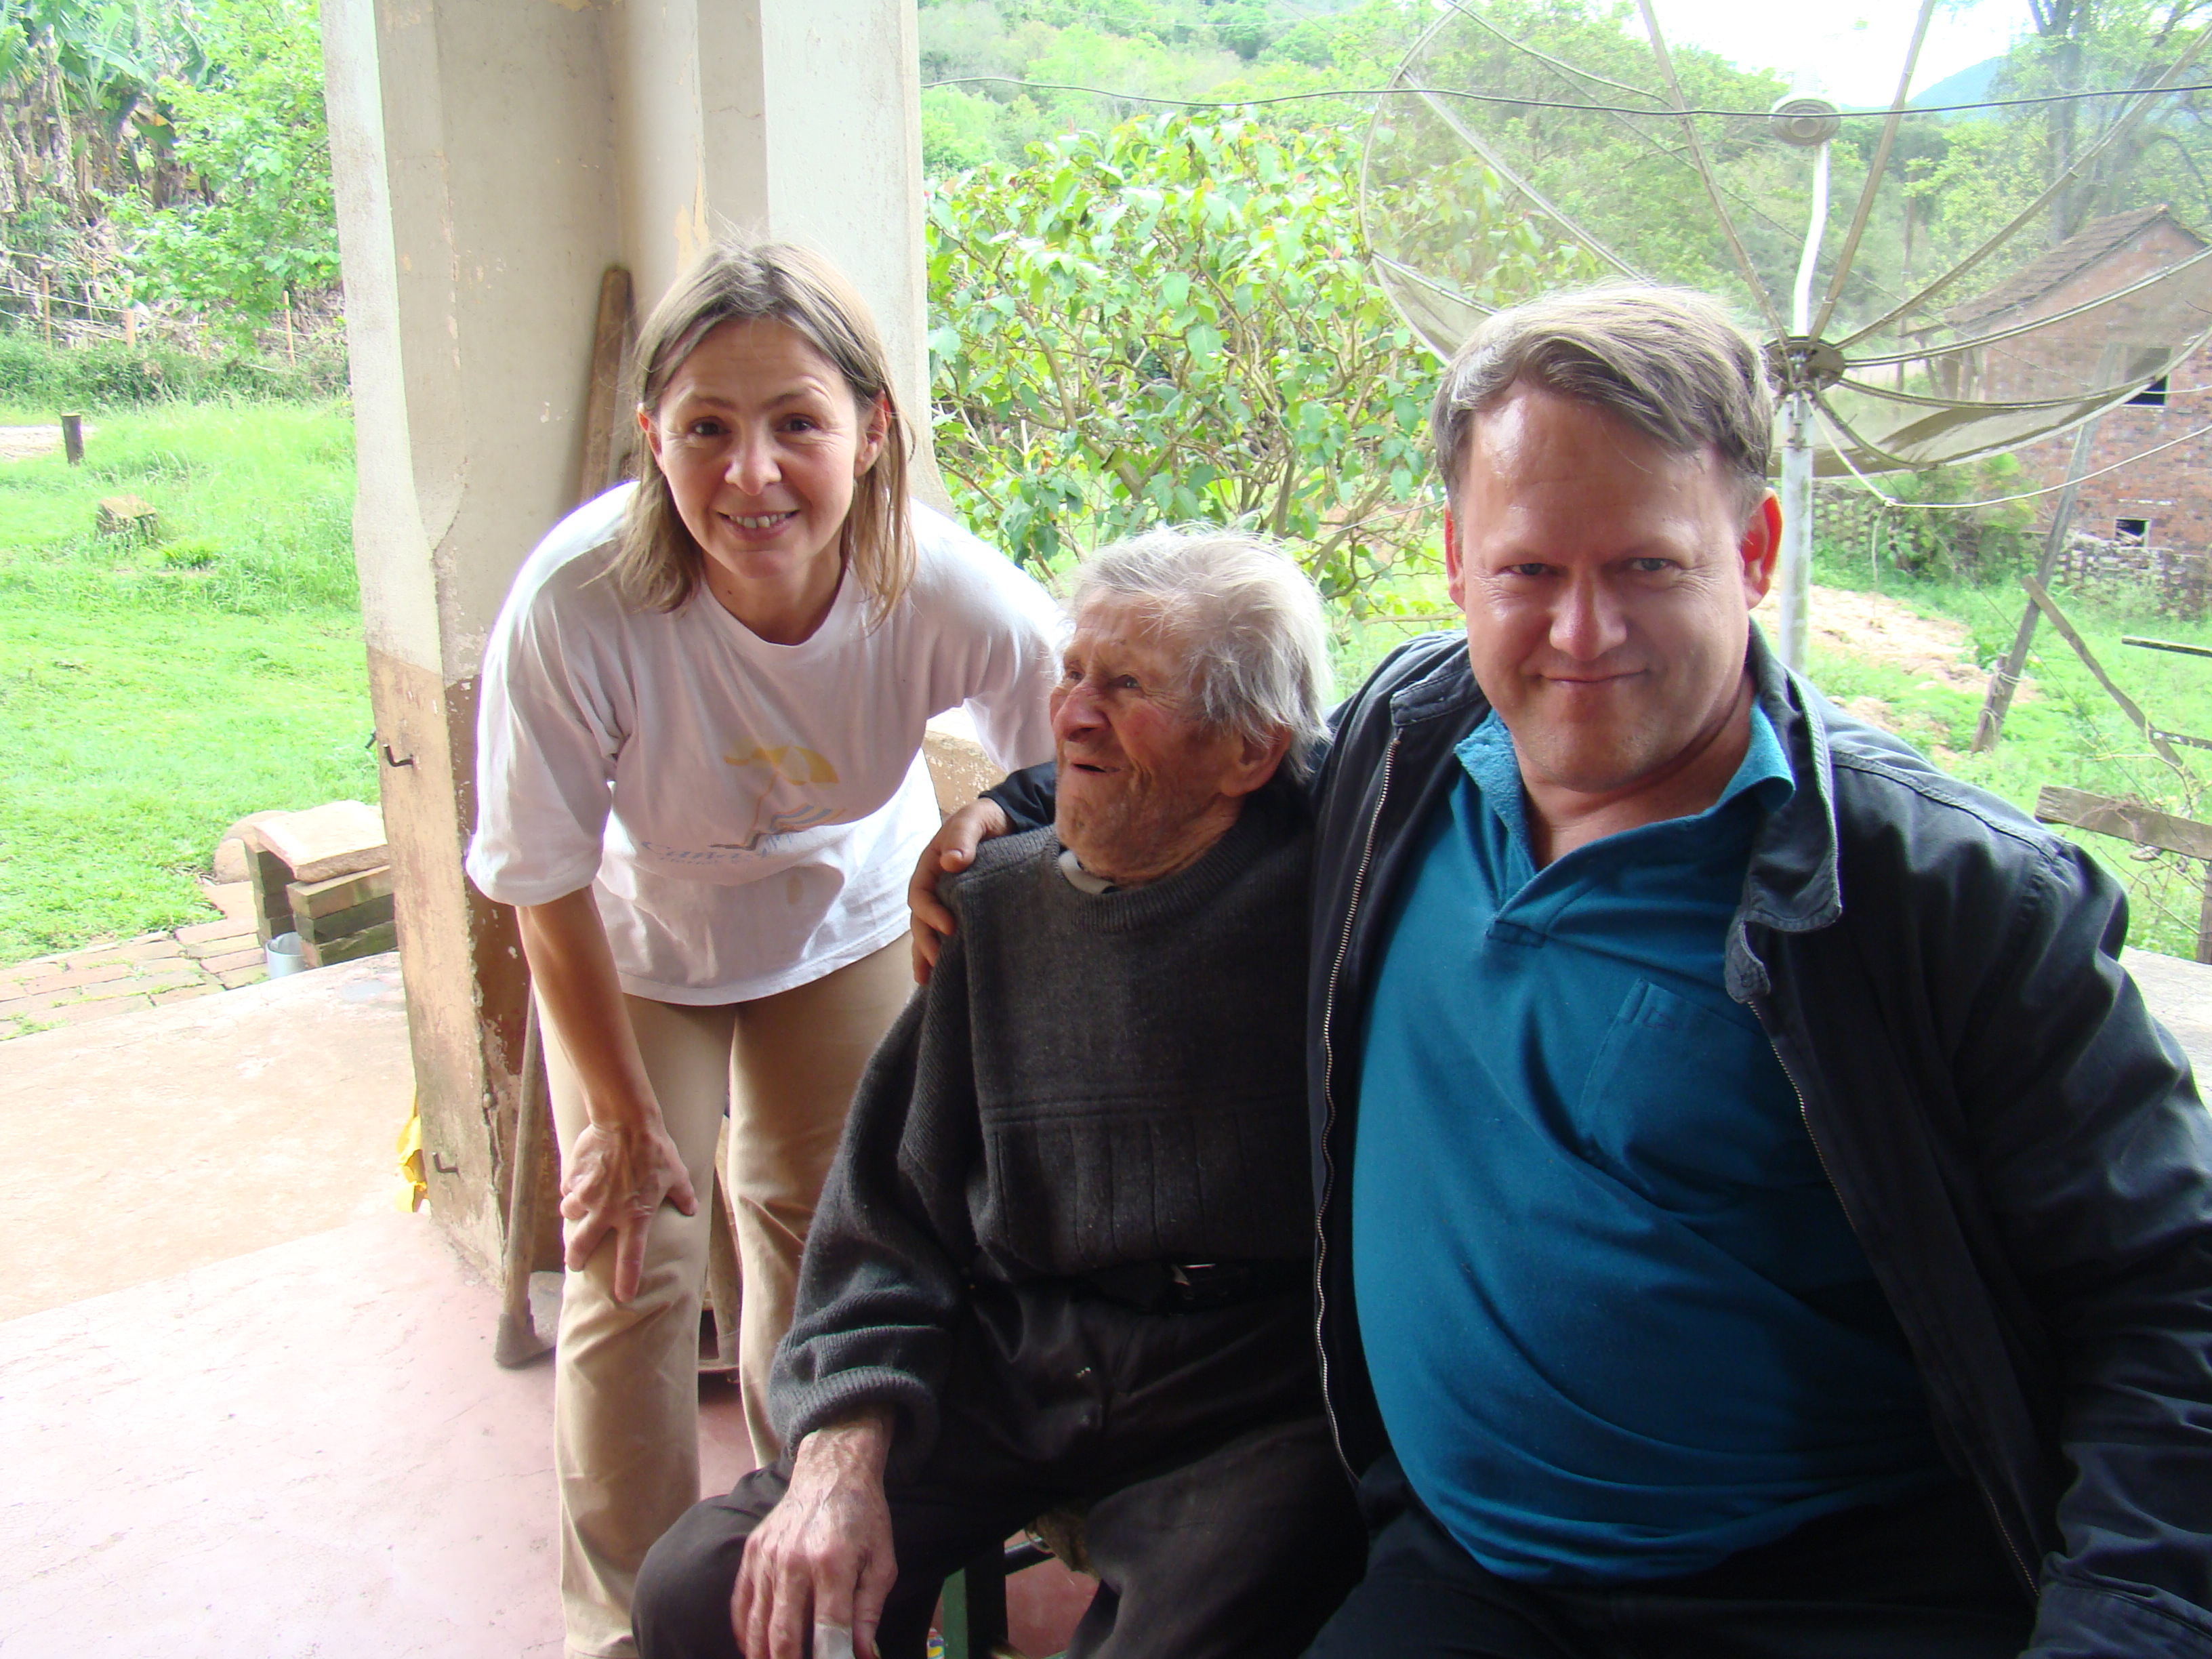
\includegraphics[width=0.85\linewidth,height=\textheight,keepaspectratio,alt={Visita ao Tio Armando Ernesto Lohmann (n.~1916), irmão de Oma Rosita, na varanda de sua casa no Vale do Taquari, em setembro de 2012.}]{imagens/lohmann_visita_tio_armando_2012.jpg}
\caption{Visita ao Tio Armando Ernesto Lohmann (n.~1916), irmão de Oma
Rosita, na varanda de sua casa no Vale do Taquari, em setembro de 2012.}
\end{figure}

Na casa do Tio Urbano, o mais velho dos que encontramos, a fotografia é
de uma varanda amarela com um vaso de orquídeas ao fundo. Ele está
sentado ao centro, de suéter estampado e calça social, as mãos grandes
cruzadas no colo e o olhar firme de um homem que já viu quase um século.
Ao lado dele, uma senhora de blusa lilás. Eu estou à esquerda, com
Matheus no colo fazendo sinal de positivo com os dois polegares, e
Lucas, de camiseta vermelha, está de pé numa cadeira de palha atrás de
nós, rindo, mais alto que todo mundo. Atrás, de pé, mais parentes da
casa. Como na garagem de Joinville, o retrato junta pontas distantes de
uma mesma linha: os meus filhos na mais nova, um tio-bisavô na mais
velha.

\begin{figure}
\centering
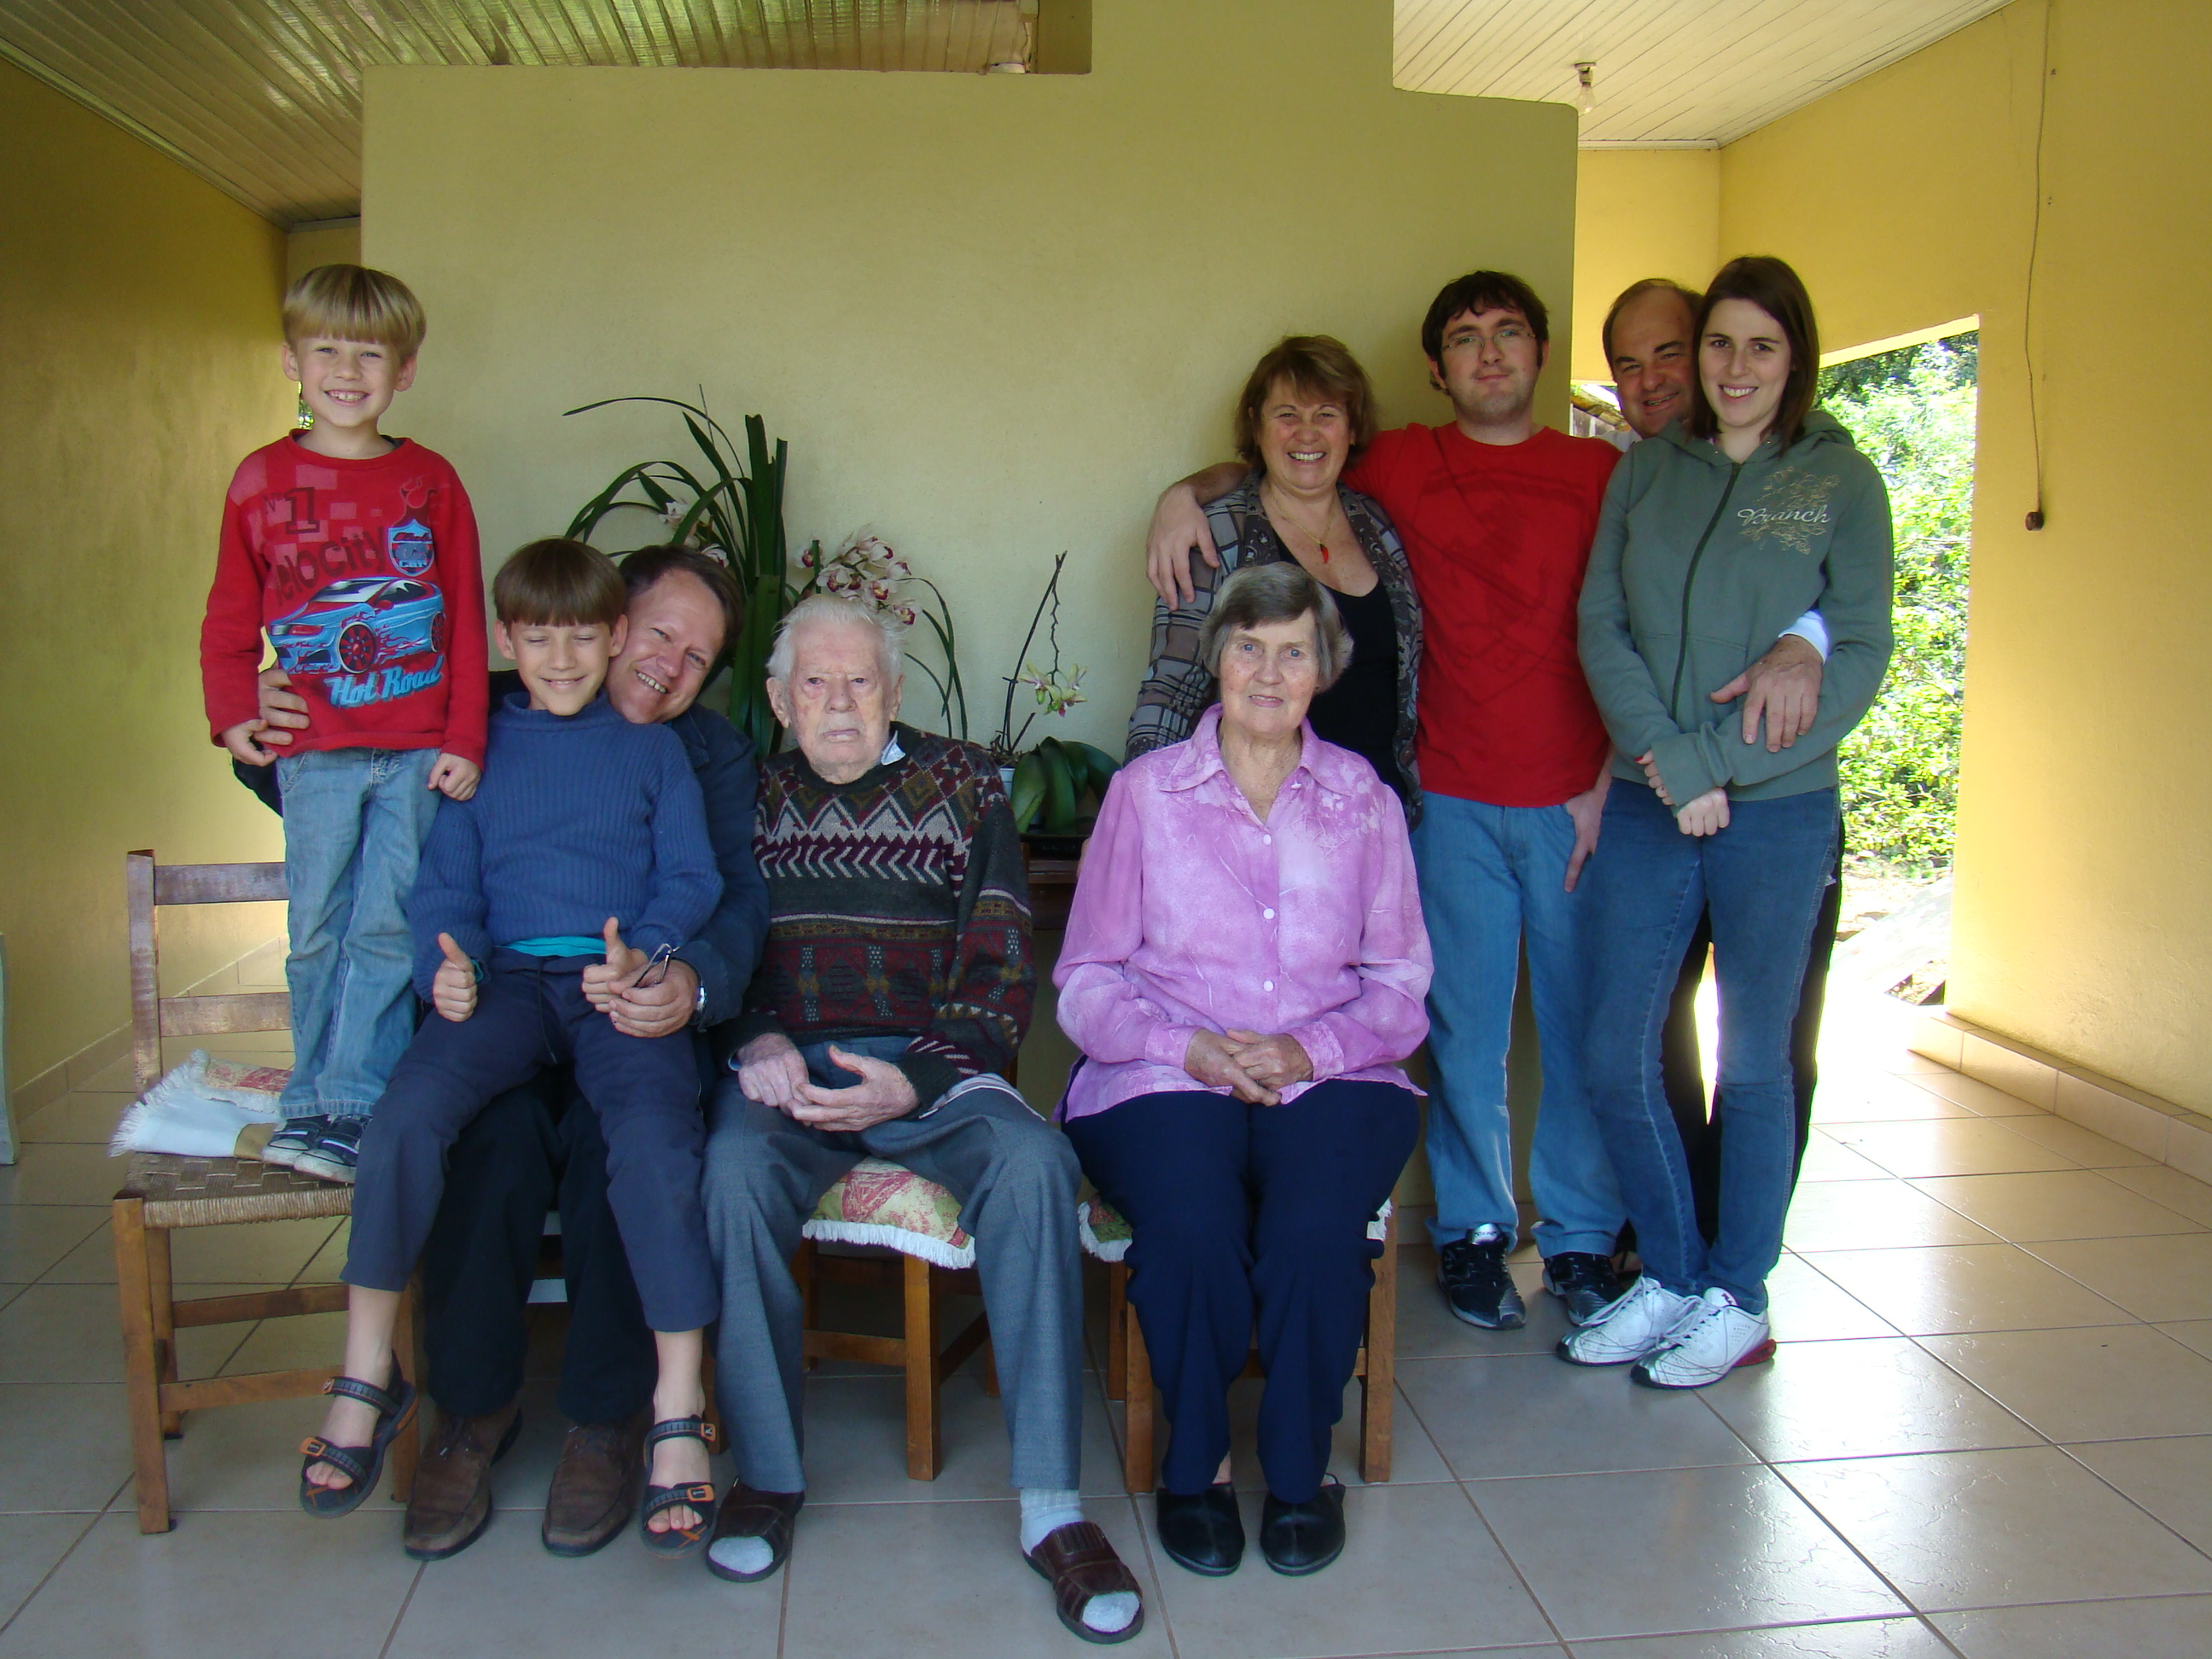
\includegraphics[width=0.85\linewidth,height=\textheight,keepaspectratio,alt={Visita ao Tio Urbano Aldo Lohmann (n.~1914), o mais velho dos irmãos de Oma Rosita que a família encontrou em setembro de 2012, com Reinaldo, Matheus e Lucas e parentes da casa.}]{imagens/lohmann_visita_tio_urbano_2012.jpg}
\caption{Visita ao Tio Urbano Aldo Lohmann (n.~1914), o mais velho dos
irmãos de Oma Rosita que a família encontrou em setembro de 2012, com
Reinaldo, Matheus e Lucas e parentes da casa.}
\end{figure}

A visita ao Tio Arlindo foi à noite, numa sala de cortinas de renda, com
o quadro de uma orquídea amarela na parede e o chão de carpete vermelho.
Na fotografia, tirada com flash, estamos todos de pé, encostados uns nos
outros como numa foto de formatura, menos uma senhora idosa que ficou
sentada no canto. Lucas está bem no meio, de camiseta vermelha, e
Matheus, de suéter azul, está à esquerda. O Tio Arlindo morreria em 7 de
fevereiro de 2018, em Estrela, um dia depois de completar noventa e
quatro anos. Na véspera, 6 de fevereiro, eu estava diante do balcão do
\emph{Standesamt} de Maxhütte-Haidhof, na Baviera, com o registro de
nascimento do meu avô nas mãos. As duas datas ficaram para sempre juntas
no meu calendário.

\begin{figure}
\centering
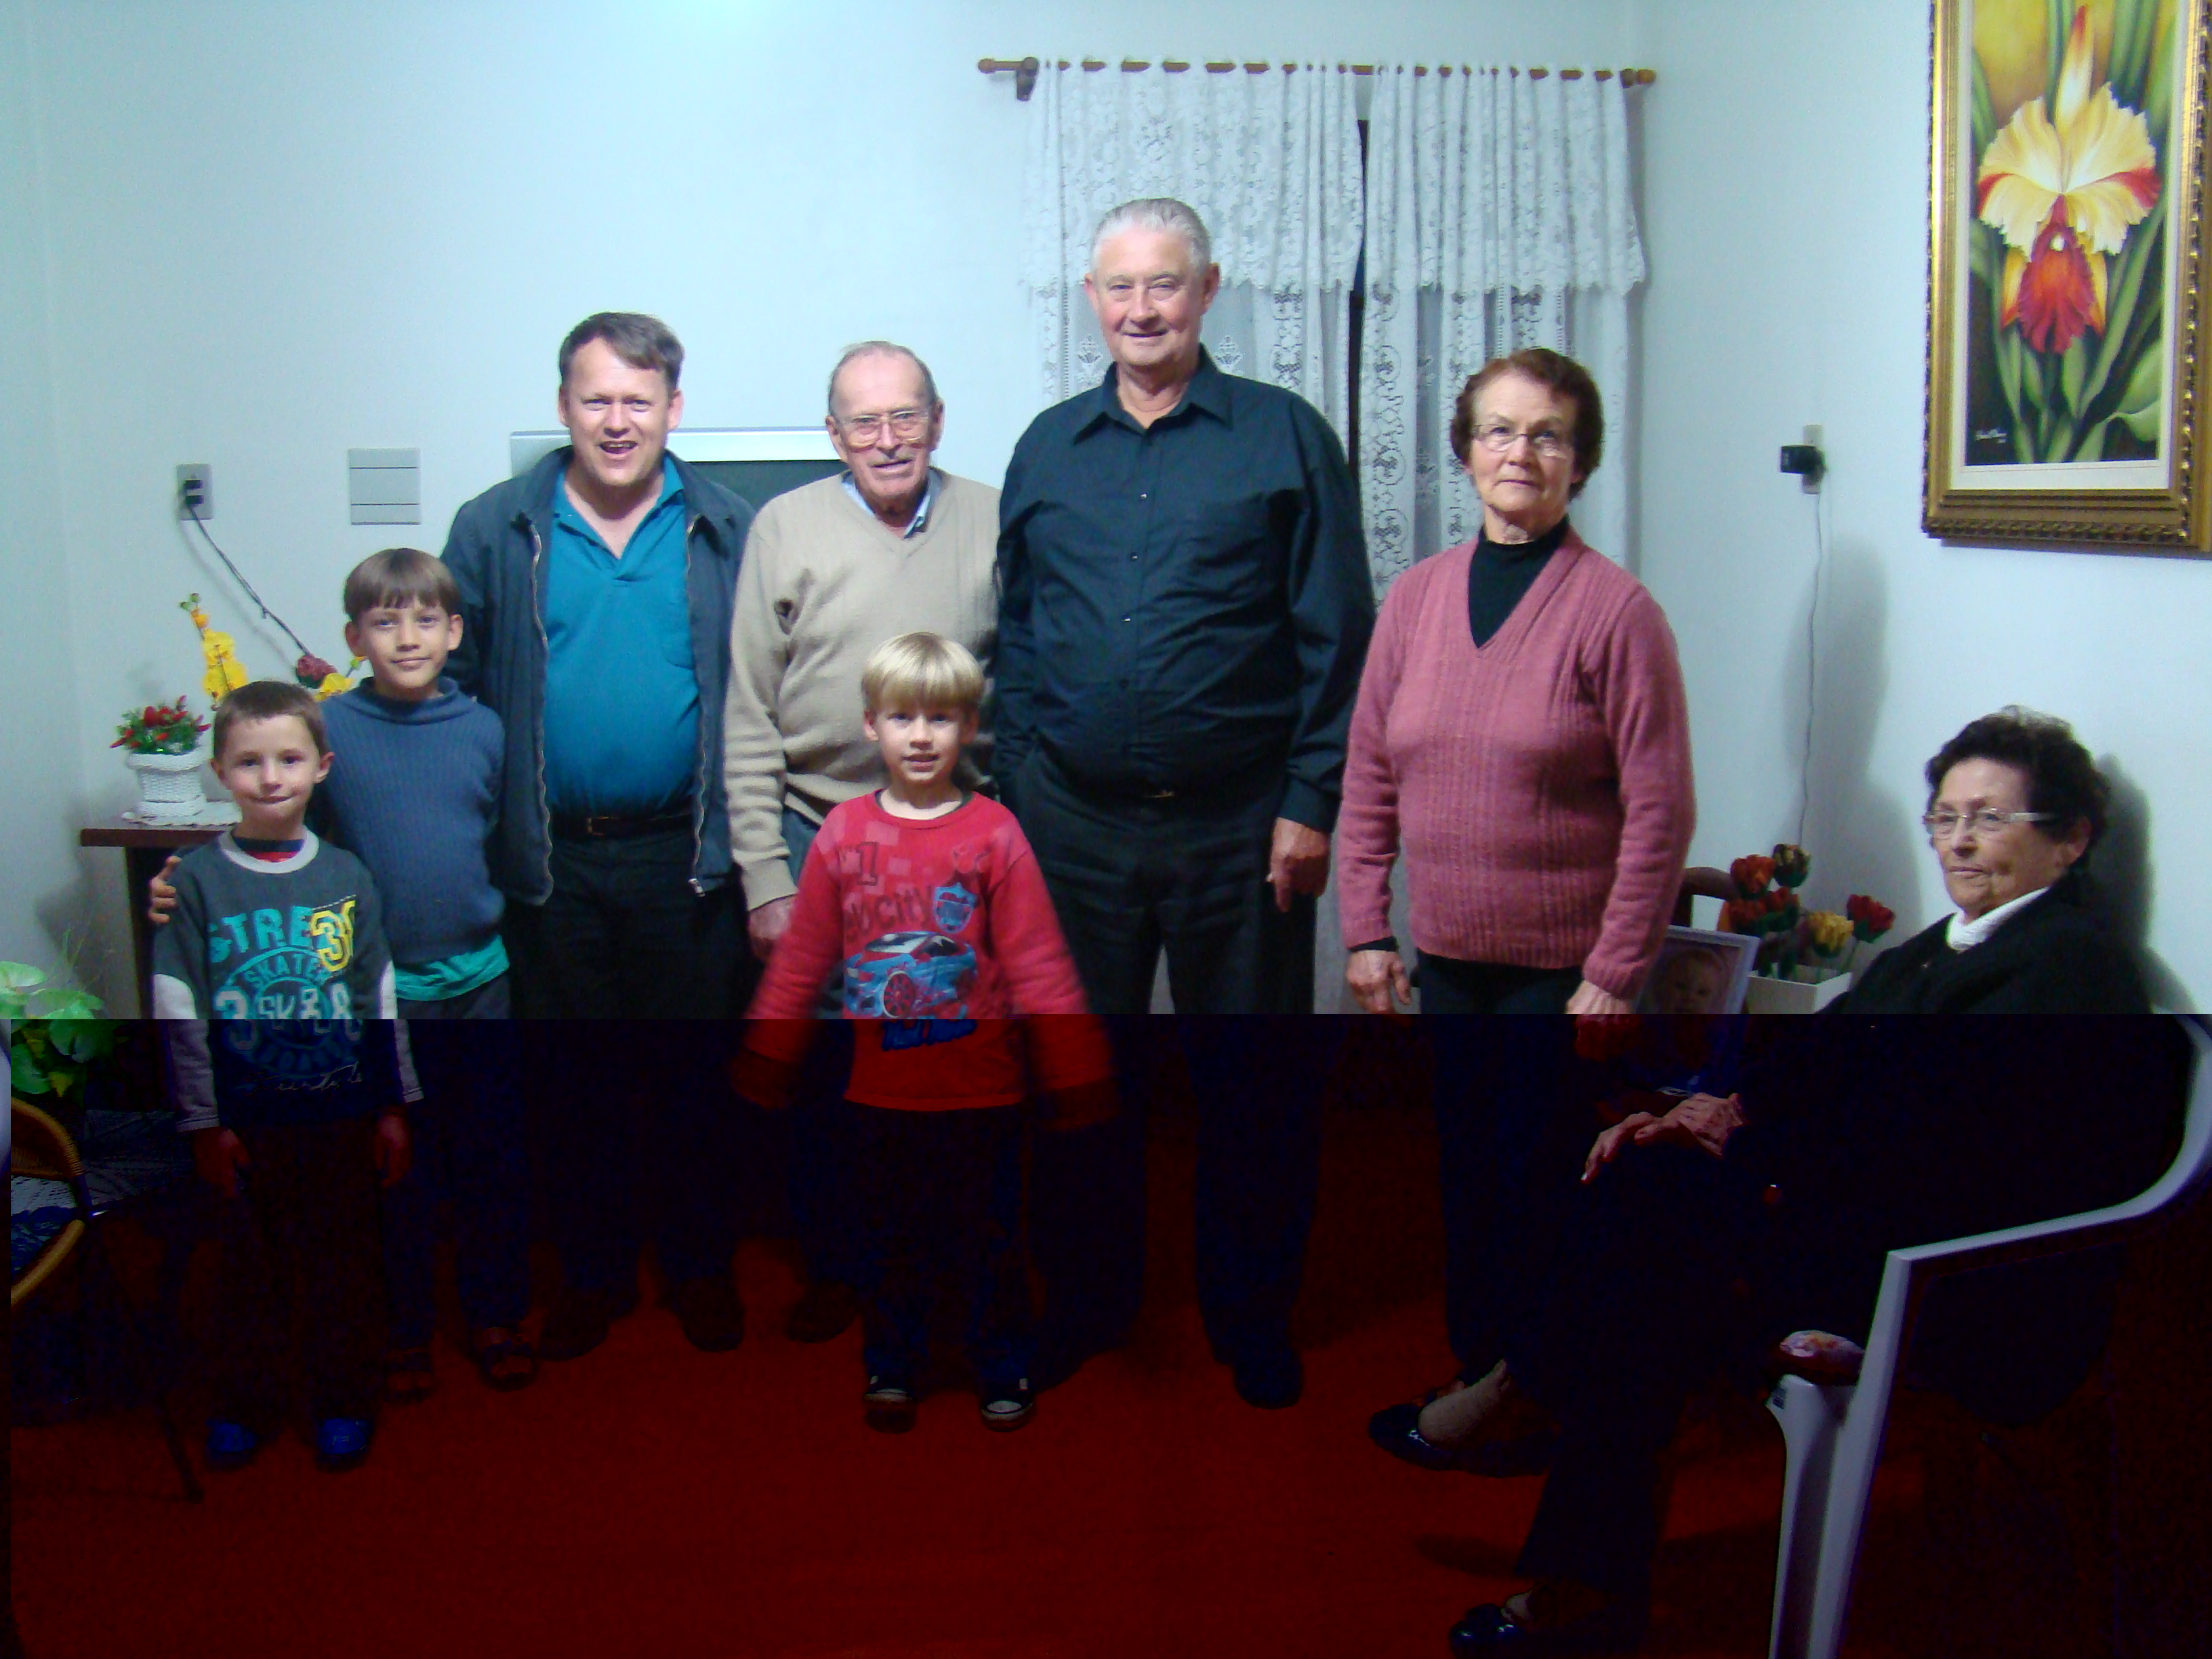
\includegraphics[width=0.85\linewidth,height=\textheight,keepaspectratio,alt={Visita ao Tio Arlindo Erno Lohmann (1924--2018), caçula dos doze irmãos, em setembro de 2012: Reinaldo, Matheus e Lucas com o tio-avô e familiares.}]{imagens/lohmann_visita_tio_arlindo_2012.jpg}
\caption{Visita ao Tio Arlindo Erno Lohmann (1924--2018), caçula dos
doze irmãos, em setembro de 2012: Reinaldo, Matheus e Lucas com o
tio-avô e familiares.}
\end{figure}

A última fotografia é a da Tia Sunta, Asunda Erna Lohmann. É a minha
preferida, por um detalhe. Ela está sentada numa poltrona de couro
gasto, num pátio de pedrisco, diante de uma casa pintada de laranja, de
mãos cruzadas e com o rosto sério de quem não gosta muito de fotografia.
Em volta, de pé e sentados, estão parentes da casa e uma moça com um
cachorrinho no colo. Matheus e Lucas estão de pé junto à porta, e a
legenda da família registra que Bárbara os acompanhava nessa visita. Em
primeiro plano, viradas para a Tia Sunta, estão quatro cadeiras vazias:
uma de plástico branco, duas de madeira, uma de praia listrada. Foi ali
que a conversa aconteceu. Quem se levantou para a fotografia deixou as
cadeiras na posição em que estavam, de frente para ela.

\begin{figure}
\centering
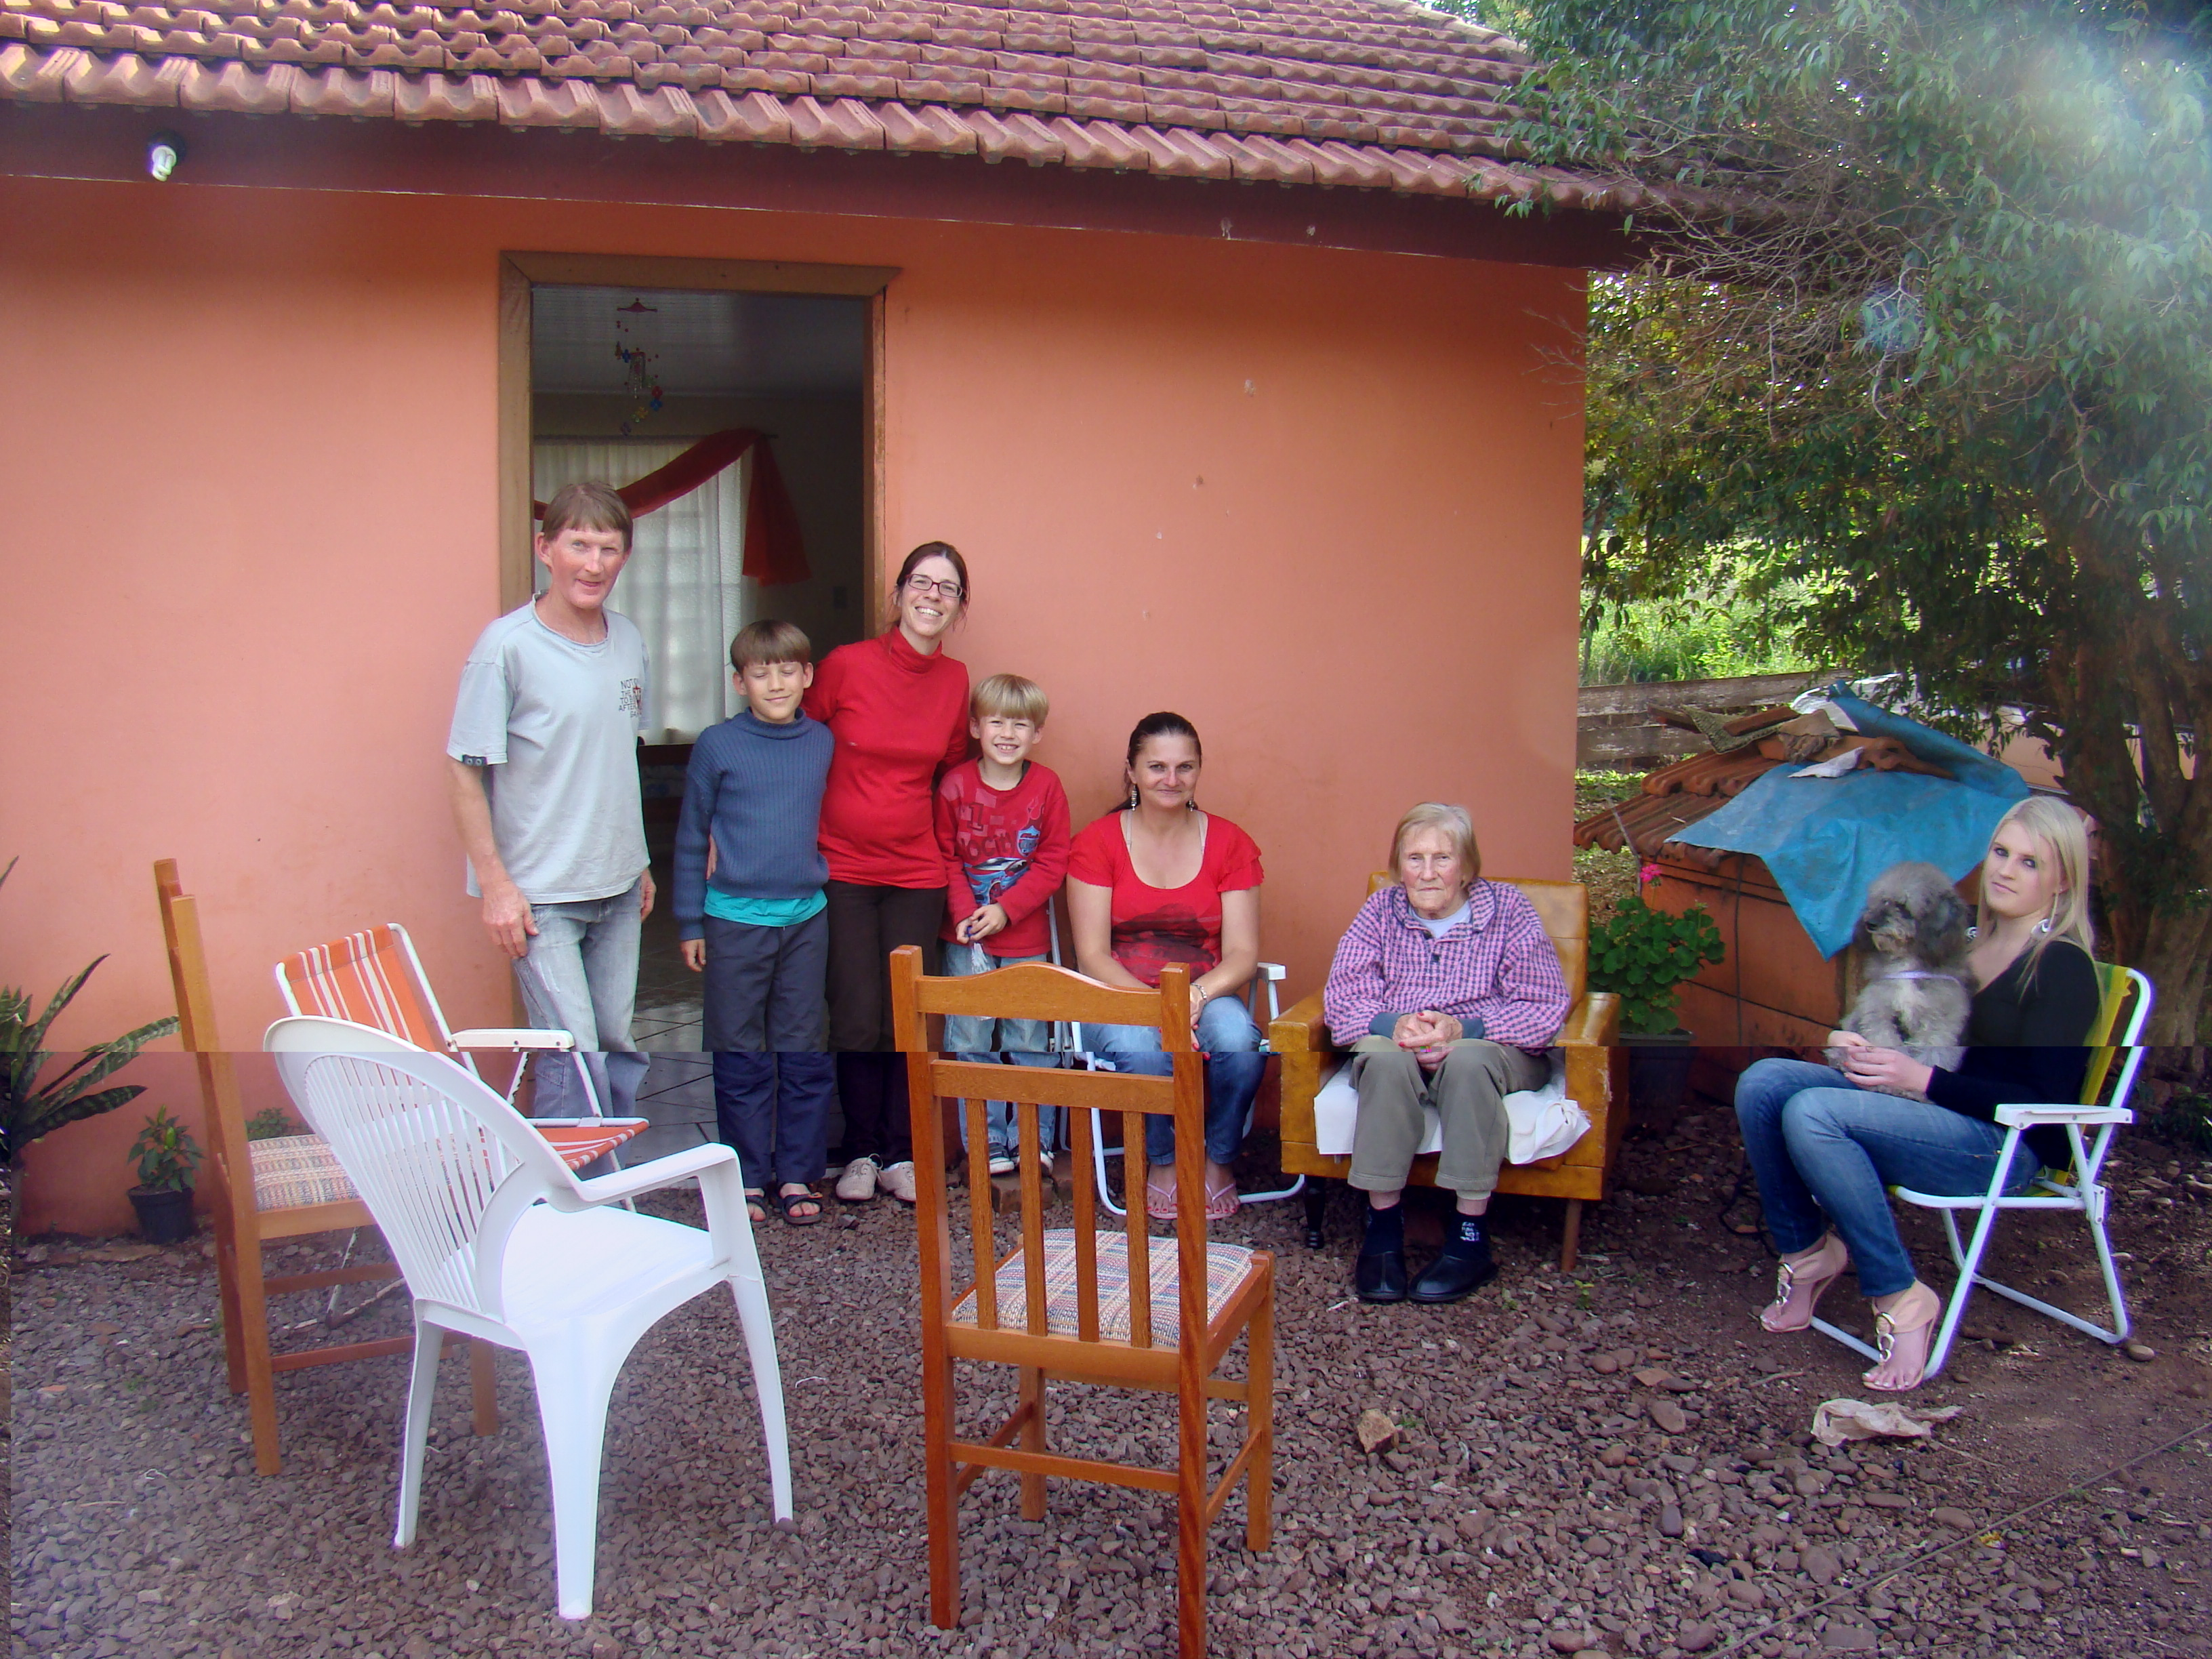
\includegraphics[width=0.85\linewidth,height=\textheight,keepaspectratio,alt={Visita à Tia Sunta (Asunda Erna Lohmann, n.~1921), irmã de Oma Rosita, em setembro de 2012, com Bárbara, Matheus e Lucas e familiares. Em primeiro plano, as cadeiras da conversa.}]{imagens/lohmann_visita_tia_sunta_2012.jpg}
\caption{Visita à Tia Sunta (Asunda Erna Lohmann, n.~1921), irmã de Oma
Rosita, em setembro de 2012, com Bárbara, Matheus e Lucas e familiares.
Em primeiro plano, as cadeiras da conversa.}
\end{figure}

Aqui Bárbara fala.

\emph{Eu não sabia bem o que ia encontrar. Eram os irmãos da minha avó,
mas eu os conhecia quase só de nome. O que me pegou foi o rosto. Em cada
um deles havia alguma coisa da Oma: o jeito de cruzar as mãos, o queixo,
o olhar meio desconfiado para a câmera. Era como ver a minha avó
repartida em quatro pessoas. Eu quis que os meninos olhassem bem, mesmo
sem entender tudo. Achei que um dia eles iam querer lembrar que
estiveram ali.}

Naqueles dias também passamos pelos cemitérios de Estrela e de Arroio do
Meio. Guardo deles menos detalhes do que gostaria, e por isso o que
escrevo nas seções seguintes sobre os túmulos se apoia também nas
fotografias e nas fichas publicadas pela CAPEF, o centro de pesquisas
genealógicas de Lajeado que reconstituiu as famílias fundadoras de
Estrela.

\section{\texorpdfstring{De Harderode ao
\emph{Hiran}}{De Harderode ao Hiran}}\label{de-harderode-ao-hiran}

\emph{Harderode, Ducado de Braunschweig, setembro de 1846}

Harderode é uma aldeia pequena nas colinas a leste do Weser, perto de
Hameln, a cidade do flautista. Ali viviam, no início do século XIX,
Johann Friedrich Christian Lohmann, nascido em 23 de outubro de 1788, e
Sophie Dorothee Elizabeth Schrader, nascida em 16 de fevereiro de 1796.
São os hexavós de vocês: sete gerações acima de Matheus e Lucas. Johann
Friedrich era professor, segundo a ficha da CAPEF, o que combina com o
orgulho que a liga dos Lohmann daquela região tinha da sua linhagem. Num
documento de 1938, essa liga dizia que, desde um certo Tönnis Lohmann,
mestre-escola e auxiliar de culto por volta de 1640, o clã dera
professores e pastores ``em todas as ramificações''. Leio esse documento
com dois cuidados. Um é a desconfiança natural diante de toda genealogia
que se gaba de si mesma. O outro é o desconforto com a data: em 1938, na
Alemanha, o interesse pelos brasões ``de linhagem'' tinha um contexto
que não posso ignorar. Mas a profissão do pai de Georg Karl Maximilian é
um fato simples, e eu o registro.

O filho deles, Georg Karl Maximilian Lohmann, nasceu em Harderode em 12
de julho de 1821. Foi comerciante. Em 4 de setembro de 1846, aos vinte e
cinco anos, embarcou para o Brasil a bordo do \emph{Hiran}. A CAPEF
conta um detalhe que eu acho extraordinário: o \emph{Hiran} era um navio
de carga, e além do capitão e da tripulação levava só dois passageiros,
Georg Karl e um senhor Berwig. Comparo com o \emph{Formosa} de 1913, que
trouxe os Haas na terceira classe com centenas de outros emigrantes, e
com os brigues de 1828 e 1847, abarrotados de famílias do Hunsrück e do
Mosela. O pentavô de vocês atravessou o Atlântico quase sozinho, entre
caixas e barris, num tempo em que a viagem durava três meses.

Imagino a travessia, e marco que é imaginação: um rapaz de Braunschweig,
filho de professor, debruçado na amurada de um cargueiro, vendo o mar
mudar de cor ao cruzar o Equador e sentindo o ar ficar mais úmido e mais
quente a cada semana. Se tinha alguma noção de meteorologia, e um filho
de professor talvez tivesse, terá aprendido na prática o que nós
ensinamos na universidade: que os alísios de nordeste empurram os
veleiros para o sul, que a calmaria equatorial os prende, que os alísios
de sudeste os levam até a costa do Brasil. O \emph{Hiran} chegou ao Rio
de Janeiro em 5 de dezembro de 1846, noventa e dois dias depois da
partida.

A ficha da CAPEF diz que era dia de aniversário da princesa Dona Isabel,
com solenidades na corte. Aqui o investigador precisa corrigir a lenda.
A princesa Isabel nasceu em 29 de julho de 1846. Em dezembro ela não
fazia aniversário, era um bebê de quatro meses. É possível que as festas
lembradas sejam as do aniversário do imperador Dom Pedro II, em 2 de
dezembro, que se estendiam por alguns dias. É possível também que o
detalhe tenha se colado à história mais tarde. Não muda nada de
essencial, mas mostra como as narrativas de família se enfeitam com o
tempo. Este livro também deve ter os seus enfeites. Espero que vocês os
encontrem.

\begin{ficha}

\textbf{Ficha do Arquivo}: Georg Karl Maximilian Lohmann (FamilySearch
\texttt{27QQ-TM9}). Nascimento: 12/07/1821, Harderode (Braunschweig).
Emigração: 04/09/1846, no cargueiro \emph{Hiran}, com um único outro
passageiro (Sr.~Berwig). Chegada ao Rio de Janeiro: 05/12/1846.
Casamento: 06/05/1849, em Kaffeeschneis (Picada Café, então São
Leopoldo), com Bárbara Wingert (05/07/1828--24/11/1915). Morte:
28/07/1899, Linha Lenz, Estrela (RS). Fonte: CAPEF, \emph{Famílias
fundadoras de Estrela --- Família Lohmann}. Ressalva: a associação da
data de chegada ao aniversário da princesa Isabel não se sustenta (ela
nasceu em 29/07/1846).

\end{ficha}

Do Rio, Georg Karl seguiu para o Sul, para a velha colônia de São
Leopoldo, fundada em 1824. Em Kaffeeschneis, a ``picada do café'' que
hoje é o município de Picada Café, casou em 6 de maio de 1849 com
Bárbara Wingert, nascida em 5 de julho de 1828. Repito o nome porque ele
me fez sorrir da primeira vez que o li. A tetravó de Bárbara também se
chamava Bárbara.

O casal teve doze filhos. Para garantir a terra deles, Georg Karl fez,
em 1870, a compra que deu nome a um lugar. Segundo a história registrada
por pesquisadoras da região, um proprietário chamado Cláudio José
Monteiro vendeu a ele vinte e quatro colônias de terra no então
município de Estrela, ao longo do rio Taquari. A CAPEF fala em cerca de
mil e duzentos hectares, o que daria colônias de uns cinquenta hectares
cada. A medida da colônia variou ao longo do tempo, e a conta não
precisa fechar ao metro. Ali nasceu a Fazenda Lohmann, que hoje é uma
localidade do município de Roca Sales, a nove quilômetros da sede. Tem
igreja evangélica com cemitério ao lado, salão de baile, uma sociedade
de cantores fundada em 1914 e a tradição dos bailes de \emph{Kerb}, com
a antiga cerveja caseira de gengibre que estourava nas garrafas. As
pesquisadoras contaram umas cento e vinte famílias, a maioria
evangélica.

Doze filhos e vinte e quatro colônias: duas colônias por filho. A conta
é tão redonda que não parece acaso. Um imigrante que viera de uma terra
onde a partilha a cada geração deixava os filhos sem chão comprou, de
uma só vez, terra suficiente para que cada filho tivesse a sua. Na
Baviera dos Haas, o herdeiro único ficava com tudo e os outros iam ser
oleiros e operários. Na Fazenda Lohmann, um pai tentou que ninguém
precisasse partir. Não conseguiu, é claro. Os netos se espalharam pelo
Vale, por Erechim, pelo Paraná, e uma bisneta acabou em Joinville.

A casa de enxaimel da família foi desmontada e reconstruída no Parque
Histórico de Lajeado, onde funciona como museu da família Lohmann.
Serviu de cenário para o filme \emph{A Paixão de Jacobina}, sobre a
revolta dos Mucker, os conflitos religiosos que abalaram a colônia de
São Leopoldo em 1874. Gosto dessa ironia: a casa de uma família luterana
bem-comportada, filmada como palco de um cisma. Georg Karl morreu em 28
de julho de 1899, na Linha Lenz, e Bárbara Wingert em 24 de novembro de
1915. Os túmulos deles estão no pequeno cemitério da Linha Winck, em
Estrela, lado a lado: primeiro o dela, depois o dele, nas fotografias da
CAPEF. O irmão de Georg Karl, Georg August Christian, que veio em 1848
com a irmã Karoline, está no cemitério de Novo Paraíso, também em
Estrela, junto da mulher, Katharina Ballus.

\section{Vinte e seis dias}\label{vinte-e-seis-dias}

\emph{Arroio do Meio, dezembro de 1889}

O terceiro filho de Georg Karl e Bárbara foi Friedrich Lohmann, nascido
em Estrela em 18 de fevereiro de 1853. É o tetravô de vocês. Ele casou
com uma moça de outra família imigrante, Suzana Regina Schnack, nascida
em 9 de julho de 1858.

Os Schnack vinham do extremo norte da Alemanha, de Schleswig-Holstein, a
terra entre dois mares. Julius Georg Schnack nasceu lá em 16 de
fevereiro de 1830, filho de Peter Friedrich Ludwig Schnack e de Regine
Marie Wacker. Casou em 8 de março de 1857 com Susanna Charlotte Köhnlein
e teve sete filhos em Estrela e Arroio do Meio. Duas das filhas casaram
com dois irmãos Lohmann: Suzana Regina com Friedrich, Elisa Sophie com
August Georg. Nas colônias isso era comum. As famílias que chegavam
juntas, que se ajudavam na derrubada e se encontravam no culto, acabavam
ligadas por mais de um fio. Julius Georg viveu até os noventa e quatro
anos e morreu em Arroio do Meio em 1924. Susanna Charlotte morreu em
1926, aos noventa e um.

A filha deles não teve a mesma sorte. Friedrich e Suzana Regina tiveram
cinco filhos: Júlio Carlos (1881), Alberto Jorge (1886), Berta
Guilhermina (1888), Adolfo André e Francisco Jacob, ambos dados como
nascidos em 1889. Francisco Jacob nasceu em 20 de novembro de 1889. Não
sei se Adolfo André era gêmeo dele ou se nasceu no começo daquele ano e
a data está errada. É uma pergunta para os livros de batismo. Em 16 de
dezembro de 1889, vinte e seis dias depois do parto, Suzana Regina
morreu em Arroio do Meio. Tinha trinta e um anos.

O registro não diz de quê. Nos anos 1880, em uma colônia do interior
gaúcho, a causa mais provável de uma morte assim, semanas depois de um
parto, era a febre puerperal, uma infecção que a medicina da época mal
compreendia e que matava mulheres jovens em toda parte. Mas é uma
hipótese. O fato é este: Friedrich ficou viúvo aos trinta e seis anos,
com cinco filhos, o mais novo com menos de um mês. Ele não casou de
novo, que eu saiba, e viveu até 1937. Quem criou Francisco Jacob? Uma
irmã mais velha, uma tia Schnack, uma vizinha com leite? Não sei. Esse
menino criado sem mãe é o rapaz de bigode do retrato de casamento de
1914.

Há uma correspondência neste livro que não planejei e que me
impressionou quando a vi. No Capítulo 10, Anna Eller morre pouco depois
do nascimento de Fernando Dörner, o caçula, por volta de 1898. Aqui,
nove anos antes, Suzana Regina Schnack morre vinte e seis dias depois do
nascimento de Francisco Jacob, o caçula. Os dois meninos órfãos de mãe
cresceram a centenas de quilômetros um do outro, sem nunca se conhecer.
Um se tornou bisavô de Bárbara, o outro, meu avô. Em vocês dois, Matheus
e Lucas, essas duas perdas se encontram.

\begin{ficha}

\textbf{Ficha do Arquivo}: \emph{Recenseamento do Brasil realizado em 1º
de setembro de 1920}, vol.~III (Agricultura), relação dos proprietários
de estabelecimentos rurais do Rio Grande do Sul (Rio de Janeiro, 1924).
Entre as ocorrências do sobrenome: ``Adolpho André Lohmann''
(provavelmente o irmão de Francisco Jacob), uma ``Linha Lohmann'',
``Frederico Lohmann'' e ``Frederico H. Lohmann'' (um deles talvez
Friedrich, então com 67 anos; não foi possível confirmar o município),
além de proprietários Schnack e Endres. A lista não identifica
parentescos; as atribuições são hipóteses.

\end{ficha}

\section{Os doze de Palmas}\label{os-doze-de-palmas}

\emph{Palmas, Arroio do Meio, meados da década de 1930}

Francisco Jacob Lohmann casou com Miguelina Leocádia Endres em 5 de
setembro de 1914. Ela nascera em 9 de dezembro de 1891, de uma família
Endres do Vale cuja história ainda não pesquisei a fundo. O censo de
1920 registra pelo menos dois proprietários Endres no Rio Grande do Sul,
mas não sei qual, se algum, era o pai dela. O casal teve doze filhos, e
a lista, que eu sei de cor de tanto conferir, merece ser escrita por
inteiro, porque é a lista dos tios-avós de Bárbara: Walter Érico,
Reinholdo, Urbano Aldo, Armando Ernesto, Walter Erich, Blanca Erna,
Albano Paulo, Rosita Érica, Eldo Astor, Asunda Erna, Dulsa Iria e
Arlindo Erno.

Devo a vocês, porém, uma confissão de investigador. As datas que os
registros dão a esses doze nomes não fecham. Walter Érico aparece como
nascido em 1911 e Reinholdo em 1912, antes do casamento de 1914. Há dois
Walter, um de 1911 e outro de 27 de dezembro de 1916, no mesmo ano de
Armando. Três filhos aparecem como nascidos em 1918, entre eles Rosita,
e dois em 1921. Algumas datas devem ser apenas aproximadas, lançadas por
alguém que as calculou de memória. E não posso descartar que os dois
Walter sejam uma só pessoa registrada duas vezes, o que é um erro
frequente nas árvores colaborativas. A família diz doze, e eu escrevo
doze, mas deixo aqui a advertência.

A fotografia mais preciosa desse ramo me ajudou a pensar o problema. É
um retrato de grupo, colorido muito tempo depois, com um papel colado
embaixo que diz: ``Família de Francisco Jacob Lohmann casado com
Miguelina Leocádia Endres Lohmann. (Foto por ocasião da conclusão da
casa nova em Palmas -- Arroio do Meio)''. Os pais estão sentados ao
centro, ela de vestido escuro com gola de renda branca, ele de terno
azul e bigode, agora grisalho, o mesmo rapaz do retrato de 1914 vinte e
tantos anos depois. Em volta, os filhos: as moças de vestido, os rapazes
de terno e gravata, duas meninas de cabelo em cuia e blusa de
marinheiro, dois meninos de camisa de botão. Contei e recontei: são
treze pessoas, os pais e onze filhos. A legenda dá os onze nomes, e
entre eles há um só Walter, o Walter Érico. Também grafa ``Urbano Arno''
onde os registros dizem ``Urbano Aldo'' e ``Reinboldo'' onde dizem
``Reinholdo''. Pela idade dos menores, o caçula Arlindo, nascido em
1924, parece ter uns dez ou doze anos, e por isso situo a foto em meados
dos anos 1930. Rosita está na ponta direita, uma moça de rosto largo e
sério, de vestido azul bordado.

\begin{figure}
\centering
\includegraphics[width=0.85\linewidth,height=\textheight,keepaspectratio,alt={A família de Francisco Jacob Lohmann e Miguelina Leocádia Endres Lohmann diante da casa nova em Palmas, Arroio do Meio (RS), provavelmente em meados da década de 1930. Segundo a legenda original, da esquerda para a direita: Blanca Erna, Armando Ernesto, Urbano, Reinholdo, Walter Érico, Arlindo Erno, Eldo Astor, Asunda Erna, Miguelina, Dulsa Iria, Francisco Jacob, Albano Paulo e Rosita Érica, a futura Oma Rosita, na ponta direita.}]{imagens/lohmann_familia_completa_palmas_arroio_do_meio.jpg}
\caption{A família de Francisco Jacob Lohmann e Miguelina Leocádia
Endres Lohmann diante da casa nova em Palmas, Arroio do Meio (RS),
provavelmente em meados da década de 1930. Segundo a legenda original,
da esquerda para a direita: Blanca Erna, Armando Ernesto, Urbano,
Reinholdo, Walter Érico, Arlindo Erno, Eldo Astor, Asunda Erna,
Miguelina, Dulsa Iria, Francisco Jacob, Albano Paulo e Rosita Érica, a
futura Oma Rosita, na ponta direita.}
\end{figure}

A outra fotografia mostra a própria casa. É um sobrado branco de telhado
alto e íngreme, com uma água-furtada, uma varanda de colunas e gradil
branco cheia de vasos, e um porão alto de alvenaria aberto para o
declive do terreno. A família está de pé, enfileirada ao longo da
fachada, pequena diante da construção. A terra em volta ainda está nua,
revolvida pela obra. Atrás, um morro de mata e o vale aberto. Imagino o
orgulho daquele dia, e aqui o verbo imaginar é honesto: um homem que
nasceu sem mãe, numa colônia onde o avô comprara vinte e quatro colônias
para os filhos, reunindo os onze ou doze filhos que tinha diante da casa
que construíra para eles.

\begin{figure}
\centering
\includegraphics[width=0.85\linewidth,height=\textheight,keepaspectratio,alt={A casa nova da família Lohmann em Palmas, Arroio do Meio, recém-concluída, com a família reunida diante da varanda. A casa fica na cota de 45 metros, em frente ao Salto do rio Taquari.}]{imagens/lohmann_casa_nova_palmas_arroio_do_meio.jpg}
\caption{A casa nova da família Lohmann em Palmas, Arroio do Meio,
recém-concluída, com a família reunida diante da varanda. A casa fica na
cota de 45 metros, em frente ao Salto do rio Taquari.}
\end{figure}

Sobre essa imagem, deixo Bárbara falar.

\emph{O que me impressiona é que todo mundo está tão arrumado para a
foto de uma casa. Os meninos de camisa abotoada, as meninas de
gravatinha de marinheiro, o bisavô de terno. Como se a casa fosse alguém
da família que acabava de chegar. E acho que era. A Oma Rosita saiu
dali, casou com um professor, foi viver em Estrela e em Nova Petrópolis
e terminou em Joinville. Mas foi naquela casa branca que ela foi moça.}

Os filhos de Francisco e Miguelina seguiram o caminho de todas as
famílias grandes da colônia. Alguns ficaram no Vale, outros partiram.
Rosita casou com Erno Hoeveler e foi viver nas escolas onde ele
ensinava. Arlindo casou em 1949 com Hilda Rahmeier e viveu e morreu em
Estrela. Os outros eu conheço só pelos nomes e pelas fotografias de
2012. Um comentário deixado por um descendente num blog de história do
Vale guarda um episódio dessa dispersão que eu não conhecia. Júlio
Carlos Lohmann, o irmão mais velho de Francisco Jacob, teria tido uma
fazenda em Erechim invadida durante a Revolução de 1923, a guerra civil
entre chimangos e maragatos. Ele, a mulher e os três filhos teriam sido
expulsos a tiros e se refugiado na Fazenda Lohmann, com o avô e os tios,
em Roca Sales, antes de se estabelecerem em Estrela. Registro como o
recebi: um depoimento de família, sem documento que o confirme. Mas ele
mostra a função que a terra comprada em 1870 continuava a ter cinquenta
anos depois: era o lugar para onde se voltava quando tudo dava errado.

\section{O rio em frente à casa}\label{o-rio-em-frente-uxe0-casa}

O Salto do Taquari, em Palmas, fica bem em frente à casa. Para quem
constrói, um rio assim é um vizinho generoso. Traz a terra fértil das
várzeas, move moinhos e foi durante muito tempo a estrada por onde os
vapores levavam as safras do Vale até Porto Alegre. Os colonos do
Taquari, como os do Itajaí e do Tubarão, assentaram-se junto à água por
boas razões.

Mas os rios do Sul têm humores longos. O Taquari nasce, com o nome de
rio das Antas, nos campos de cima da serra, e recolhe a chuva de uma
bacia enorme de encostas íngremes. Quando uma frente fria se arrasta
devagar sobre o Rio Grande, alimentada pela umidade que o jato de baixos
níveis traz da Amazônia pelo leste dos Andes, ou quando um ciclone
extratropical se forma sobre o estado e despeja num dia a chuva de um
mês, essa água toda converge para o vale em poucas horas. O rio sobe
metros. É uma meteorologia que conheço bem, porque passei boa parte da
vida profissional tentando prevê-la e modelá-la, no Itajaí e no Taquari.

Em maio de 1941, poucos anos depois da fotografia da casa nova, o
Taquari teve uma das maiores cheias da sua história registrada. Toda a
bacia do Guaíba transbordou, e Porto Alegre ficou semanas debaixo
d'água. Os doze irmãos de Palmas tinham então entre dezessete e trinta
anos. É muito provável que todos tenham guardado na memória aquela água
subindo pelo vale, e que a cheia de 41 tenha se tornado, como para todas
as famílias do Taquari, a medida de todas as outras. Não tenho, porém,
nenhum relato deles sobre isso. Não perguntei em 2012. Hoje eu
perguntaria primeiro.

O perfil topográfico que fiz anos depois põe a Casa Lohmann na cota de
quarenta e cinco metros, de frente para o Salto. Desenhei nesse perfil
as linhas das grandes cheias, a de 1941 e as que vieram depois. Não vou
contar aqui o que o desenho mostra. Essa história pertence ao próximo
capítulo, junto com a do Tubarão e a do Itajaí, porque as três são a
mesma história. Digo apenas o que todo mundo no Brasil soube pelos
jornais. Em setembro de 2023, um ciclone extratropical despejou sobre o
Vale do Taquari uma chuva que matou dezenas de pessoas, e Roca Sales,
onde fica a Fazenda Lohmann, Muçum e Arroio do Meio, onde fica Palmas,
foram arrasadas. Em novembro de 2023 o rio voltou a subir. Em maio de
2024, na maior catástrofe climática da história do Rio Grande do Sul,
subiu outra vez, mais alto do que todos lembravam.

O Tio Arlindo já não estava vivo para ver. Morreu em fevereiro de 2018,
no mesmo mês em que eu abria os livros de Maxhütte-Haidhof. Dos outros
irmãos, não sei as datas, e não vou supor. Mas quando vi pela televisão,
em 2023 e em 2024, as imagens de Roca Sales e de Arroio do Meio cobertas
de lama, a primeira coisa que fiz foi procurar no mapa duas coordenadas:
a da Fazenda Lohmann e a da casa branca diante do Salto. Depois fui
procurar as fotografias de setembro de 2012, as varandas, as cadeiras em
roda, os quintais de pedrisco. Eram os mesmos lugares.

Aqui Bárbara encerra a Parte IV.

\emph{Olho o perfil da casa, com as linhas das cheias desenhadas por
cima, e custo a juntar as duas imagens. Aquela casa é a da foto em que
todo mundo está de roupa de domingo. Pensei nos meus tios-avós, nas
cadeiras em volta da Tia Sunta, e pensei que a gente tinha chegado a
tempo de ver as pessoas, mas não sabia que também estava chegando a
tempo de ver os lugares como eles eram.}

Vocês dois, Matheus e Lucas, estiveram nesses lugares quando eram
pequenos. Estão nas fotografias, de camiseta vermelha e de suéter azul,
no colo de um pai e em pé numa cadeira, ao lado de tios que tinham
nascido antes da Primeira Guerra. Talvez não se lembrem. Por isso
escrevi este capítulo. O próximo começa por onde este termina: pela água
que sobe e pelas famílias que, há quase dois séculos, constroem as casas
na beira dela.

\section{Para vocês descobrirem}\label{para-vocuxeas-descobrirem-11}

\begin{itemize}
\tightlist
\item
  Adolfo André era gêmeo de Francisco Jacob, ou nasceu no começo de 1889
  e a data está errada? Os livros de batismo podem dizer.
\item
  Quem criou Francisco Jacob depois da morte de Suzana Regina, em 16 de
  dezembro de 1889?
\item
  Houve dois Walter entre os filhos de Francisco e Miguelina, ou um só,
  registrado duas vezes? A legenda da fotografia de Palmas traz só o
  Walter Érico.
\item
  O que os irmãos de Palmas guardaram da cheia de maio de 1941? Eu não
  perguntei em 2012. Perguntem aos descendentes do Tio Urbano, do Tio
  Armando, da Tia Sunta e do Tio Arlindo.
\end{itemize}

\part{Três Rios, o Clima e uma
Herança}\label{truxeas-rios-o-clima-e-uma-heranuxe7a}

\begin{boletim}

Alerta hidrológico para as bacias do Tubarão, do Itajaí e do Taquari;
granizo na Ilha. Tempo de retorno: uma geração.

\end{boletim}

\chapter{Três Rios, Uma Só Chuva}\label{cap-13}

\emph{28,5° S · 49,0° O, Tubarão, SC · 27,4° S · 49,6° O, Ituporanga, SC
· 29,3° S · 51,9° O, Palmas, Arroio do Meio, RS}

\begin{quote}
\emph{Um rio não esquece o caminho; quem esquece somos nós.}
\end{quote}

A pior enchente que Santa Catarina tinha conhecido até então chegou em
1974, num ano de La Niña, quando, em tese, o Sul devia estar mais seco.

\section{O mapa sobre a mesa}\label{o-mapa-sobre-a-mesa}

Há um mapa que nunca saiu da minha cabeça desde que comecei esta
investigação, e ele não tem fronteiras de município nem nomes de
paróquia. É um mapa de bacias hidrográficas. Se eu o estendo sobre a
mesa da cozinha, como fiz tantas vezes com as cartas sinóticas que os
meninos viam espalhadas pela casa, aparecem três linhas azuis que descem
da serra para o mar e, ao lado de cada uma, um punhado de sobrenomes.

A primeira é o rio Tubarão, que desce da Serra Geral e se derrama nas
lagoas de Laguna. Foi por Laguna, diz a tradição da família, que Johann
e Maria chegaram a Santa Catarina em 1913; os documentos, por enquanto,
só garantem que desembarcaram no Rio de Janeiro. A segunda é o Itajaí,
com seus três braços que se juntam no Alto Vale, onde o \emph{Fata} e a
\emph{Mota} derrubaram mata em Rio Novo, ergueram a matriz de
Ituporanga, envelheceram em Aurora e onde meu pai, Baldoíno, foi viver
em Vidal Ramos. Um pouco ao lado corre o Itajaí-Mirim, que passa por
Brusque, onde dormem Fernando Dörner e Gertrudes Preiss, os pais de
minha mãe. A terceira linha azul é o Taquari, no Rio Grande do Sul, que
nasce como rio das Antas nos campos de cima da serra e desce encaixado
entre paredões até se abrir em várzea na altura de Roca Sales, Arroio do
Meio, Lajeado e Estrela. Ali ficam a Fazenda Lohmann, a casa de Palmas,
os túmulos da Linha Lenz e quase tudo o que Bárbara herdou do lado da
avó.

Durante anos olhei para essas três linhas como genealogista. Só depois,
um pouco envergonhado da demora, percebi que as olhava também como
meteorologista. Os três rios que atravessam a história dos meus filhos
são três dos rios mais estudados do Sul do Brasil, justamente porque
estão entre os que mais transbordam. Cada um deles tem a sua
enchente-assombração, aquela que os velhos citam pelo ano, sem precisar
dizer mais nada: ``a de 74'', ``a de 83'', ``a de 41''. Nos últimos
anos, cada um ganhou uma nova data para pôr ao lado da antiga.

Meu trabalho na universidade gira, há muito tempo, em torno de prever
essas águas: modelos que dizem quanto vai chover, que transformam chuva
em vazão e espalham a vazão sobre o terreno. Este não é um relatório
técnico, mas não posso escrever sobre esses três vales fingindo que não
sei o que sei. Seria como descrever o retrato de casamento de Francisco
e Miguelina sem dizer que ele está pendurado numa parede que a água já
alcançou.

O título deste capítulo é uma provocação de professor. Não houve uma
única chuva sobre Tubarão em 1974, o Itajaí em 1983 e o Taquari em 2024.
Mas há uma única máquina que fabrica essas chuvas, e antes de visitar
cada rio preciso abrir a tampa dela.

\section{A máquina da chuva}\label{a-muxe1quina-da-chuva}

Imaginem, como peço aos meus alunos, um rio que não se vê. A leste dos
Andes, entre a Bolívia, o Paraguai e o norte da Argentina, corre em
certas épocas uma faixa estreita de vento forte a pouco mais de um
quilômetro de altura. Os meteorologistas a chamam de jato de baixos
níveis. Ele nasce do ar quente e úmido da Amazônia, que os alísios
empurram para oeste até bater na muralha andina; sem conseguir passar, o
ar se dobra para o sul e escorre ao longo da cordilheira como água ao
longo de uma calha. É um rio aéreo, e carrega mais água em forma de
vapor do que muitos rios de verdade carregam no leito. Quando esse jato
chega ao sul do continente e encontra algum mecanismo que force o ar a
subir, o vapor se condensa e a Amazônia cai em forma de chuva sobre o
Paraguai, o Rio Grande do Sul e Santa Catarina.

O mecanismo que força a subida mais comum por aqui é a frente fria. Uma
massa de ar polar avança do sul, mais densa, e se mete por baixo do ar
tropical como uma cunha, levantando-o. Na maior parte das vezes a frente
passa: chove um dia, o vento vira para sul, o céu limpa e a temperatura
cai. O perigo está nas frentes que param. Quando o ar frio não tem força
para seguir e o ar quente não tem força para empurrá-lo de volta, a
frente fica estacionada por dias sobre a mesma faixa de terra, com o
jato de baixos níveis alimentando-a por trás, como uma mangueira que
alguém esqueceu aberta. É a chamada frente semiestacionária, e ela tem o
péssimo hábito de se alinhar com as bacias do Sul.

O terceiro personagem é o ciclone extratropical. Ao longo das frentes,
sobretudo perto da costa do Uruguai e do Rio Grande do Sul, a pressão às
vezes despenca e o ar começa a girar em sentido horário, que é o sentido
dos ciclones no hemisfério sul. Um ciclone desses organiza toda a
umidade em volta, puxa o ar do norte por um lado, o ar do sul pelo
outro, e pode despejar em um dia o que normalmente cairia em um mês. Foi
um ciclone assim que, nos primeiros dias de setembro de 2023, se
instalou sobre o Vale do Taquari.

O quarto personagem todo catarinense já ouviu no noticiário: El Niño. A
cada poucos anos, as águas do Pacífico equatorial, na altura do Peru e
do Equador, ficam mais quentes do que o normal. Parece longe, mas o
oceano aquecido muda o lugar onde a atmosfera tropical sobe e desce, e
essa mudança se propaga até o nosso céu. No Sul do Brasil, anos de El
Niño tendem a ser mais chuvosos, sobretudo no inverno e na primavera,
com frentes que estacionam com mais frequência e um jato subtropical
mais forte segurando os sistemas sobre nós. A irmã inversa, La Niña, de
águas frias no mesmo Pacífico, costuma deixar o Sul mais seco.

Costuma. Há uma frase que repito até que os alunos a decorem: \emph{o
clima não é destino}. O El Niño vicia o baralho, mas não escolhe a
carta. Torna certos invernos mais propensos a enchentes, como um baralho
com mais cartas vermelhas torna mais provável tirar copas; ainda assim,
sai espadas, e sai copas também em baralhos que ninguém viciou. Os três
vales da família me dão, cada um, uma lição sobre essa frase.

Falta um último mecanismo, que é o mais catarinense de todos: a serra. O
ar que chega do mar carregado de umidade, ao bater na escarpa da Serra
Geral ou nas encostas da Serra do Mar, é obrigado a subir. Subindo,
esfria; esfriando, condensa; condensando, chove. É a chuva orográfica.
Em Santa Catarina, onde a serra fica a poucas dezenas de quilômetros do
mar, ela pode virar protagonista. Foi o que aconteceu em novembro de
2008.

\section{Tubarão, 1974: a foz onde tudo
começou}\label{tubaruxe3o-1974-a-foz-onde-tudo-comeuxe7ou}

\emph{Tubarão, Santa Catarina, 24 e 25 de março de 1974}

Chovia havia dias sobre a encosta da serra, e a chuva não se movia. O
rio Tubarão, que desce encaixado entre morros até ganhar a planície,
subiu, pelo que contam os relatos da época, durante a noite de domingo
para segunda, e não parou mais de subir. A cidade fica numa planície
baixa, cortada pelo rio e debruçada sobre ele, e a água entrou de uma
vez. As fotos da época mostram telhados como ilhas, pessoas sobre
caixas-d'água, barcos onde antes havia rua, e um mar de lama castanha
que levou semanas para baixar. Os números oficiais mais citados falam em
cerca de duzentos mortos e dezenas de milhares de desabrigados. Até
então, foi o maior desastre natural da história de Santa
Catarina.\footnote{Os números de mortos e desabrigados de 1974 variam
  conforme a fonte; uso aqui os valores oficiais mais citados, sem
  pretender precisão.}

Eu tinha oito anos. Não posso, em honestidade, dizer o que senti, porque
não tenho lembrança fiel daqueles dias que não esteja contaminada pelo
que aprendi depois. Mas sei o que o episódio significou para quem, como
eu, viria a estudar a atmosfera no estado: a enchente de Tubarão virou
uma espécie de marco zero da consciência catarinense sobre cheias.
Depois dela o rio foi retificado e canalizado; o meandro que antes
serpenteava pela cidade foi cortado e trocado por um leito mais reto,
mais rápido, contido por diques. Uma geração inteira cresceu ouvindo que
aquilo não se repetiria.

O detalhe que mais me intriga como meteorologista é que 1973 e 1974 eram
anos de La Niña. O baralho estava, em tese, viciado a favor da seca no
Sul. No entanto, uma situação de chuva persistente sobre a encosta,
alimentada pela umidade do oceano e travada pelo relevo, bastou para
produzir a pior tragédia que o estado havia conhecido. Quando digo aos
alunos que o clima não é destino, é Tubarão que tenho em mente: o ano
``favorável'' não protegeu ninguém.

Aqui o mapa genealógico se dobra sobre o hidrológico de um jeito que
ainda me dá frio. O Tubarão termina em Laguna. É pelas lagoas de Laguna
que ele chega ao mar, e é por esse canal que, sessenta e um anos antes,
segundo a tradição da família, Johann e Maria teriam entrado em Santa
Catarina. Quando estivemos em Laguna, em fevereiro de 2012, Matheus
tinha nove anos e Lucas, seis. Para eles, imagino, era uma praia de
férias. Eu olhava a água das lagoas pensando em duas coisas que, até
então, guardava em gavetas separadas: uma família de bávaros que talvez
tenha desembarcado ali, com uma filha prestes a nascer e duas crianças
pequenas, e um rio que, em 1974, despejou naquelas mesmas lagoas tudo o
que arrancou de uma cidade.

Não há relação de causa entre uma coisa e outra; há apenas o lugar.

\section{Itajaí: o vale do Fata e da
Mota}\label{itajauxed-o-vale-do-fata-e-da-mota}

O Itajaí é o rio da minha infância e o rio do meu ofício. Ele nasce em
três braços. O Itajaí do Oeste desce por Taió e Rio do Oeste; o Itajaí
do Sul desce por Ituporanga e Aurora; o Itajaí do Norte, que muita gente
ainda chama de Hercílio, vem de José Boiteux e Ibirama. O do Oeste e o
do Sul se encontram em Rio do Sul, o do Norte se junta um pouco abaixo,
e dali em diante o rio único corre para Blumenau, Gaspar, Ilhota e
Itajaí, onde encontra o mar. O Itajaí-Mirim, seu afluente mais
conhecido, nasce nos morros de Vidal Ramos, passa por Brusque e se junta
ao rio principal já perto da foz.\footnote{Simplifico a geografia das
  sub-bacias; os pontos exatos de nascente e de confluência de cada
  braço são descritos de modos ligeiramente diferentes em fontes
  distintas.}

Se eu marcar nesse mapa os lugares da família de meu pai, quase todos
caem sobre uma linha azul. Rio Novo, onde o \emph{Fata} derrubou mata a
machado e onde nasceram Agnes, Elza, Baldoíno e Maria, é terra do Itajaí
do Sul. Ituporanga, onde ele e os filhos ergueram a Igreja Matriz, a
Casa Paroquial, o Seminário e a ampliação do Hospital das Irmãs, fica à
beira do mesmo rio. Ribeirão das Pacas, em Aurora, onde os dois
envelheceram e onde estão sepultados entre os túmulos que ele próprio
moldou, está um pouco abaixo. Vidal Ramos, para onde meu pai foi, é
cabeceira do Itajaí-Mirim; Brusque, onde morreram os pais de minha mãe,
é o mesmo Mirim, mais largo e mais perigoso, alguns dias de água abaixo.
Se uma gota de chuva cair sobre a casa de meus pais e não for evaporada
no caminho, ela passa por Brusque antes de chegar ao mar.

O Itajaí transbordava muito antes de os Haas chegarem. Blumenau guarda a
memória de grandes cheias em 1880, quando a colônia ainda era jovem, e
em 1911, dois anos antes de o \emph{Formosa} zarpar de Marselha. Imagino
que, se a notícia tivesse chegado à Baviera, não teria mudado nada:
ninguém escolhe o destino pela estatística de enchentes, e sim pela
promessa de terra.

As enchentes que eu ouvi contar, e que depois estudei, foram as de 1983
e 1984. Em julho de 1983, durante um dos El Niños mais fortes do século,
o rio passou de quinze metros em Blumenau; no ano seguinte, em agosto de
1984, subiu um pouco mais.\footnote{As cotas de Blumenau são as da régua
  histórica da cidade, cerca de 15,3 m em 1983 e 15,5 m em 1984. Prefiro
  não arredondar para mais.} A de 1983 é o caso exemplar da máquina de
que falei: um El Niño intenso no Pacífico, um jato subtropical forte
sobre o Sul, frentes que chegavam e não iam embora, semanas de chuva
sobre um solo que já não absorvia nada. Uso esse caso em sala. A de
1984, um ano depois, quando o Pacífico já não estava no mesmo estado, é
o contraponto que gosto de mostrar logo em seguida: outra vez a
advertência de que o dado carregado não é o único dado na mesa.

Depois veio novembro de 2008, que é, para mim, a enchente mais difícil
de explicar a quem não é do ramo, justamente porque não se parece com as
outras. Não houve um grande rio subindo lentamente por semanas; houve
uma chuva teimosa, vinda do mar. Um anticiclone posicionado sobre o
Atlântico empurrou durante dias um fluxo de leste, úmido, contra a
encosta da serra e dos morros do Vale. O ar, forçado a subir, despejou
chuva sem trégua sobre um terreno já encharcado. Os morros começaram a
ceder. Morro do Baú, Ilhota, Gaspar, bairros de Blumenau: os nomes
daquele novembro são nomes de deslizamentos, não apenas de cotas.
Morreram cerca de cento e trinta e cinco pessoas em Santa Catarina.
Brusque, no Itajaí-Mirim, também foi atingida, como já o fora em 1984 e
voltaria a ser em 2011, o mesmo ano em que Rio do Sul, no encontro dos
três braços do Alto Vale, viu a água subir mais uma vez sobre o seu
centro.

Para quem faz previsão, 2008 deixou uma lição de humildade. Prever chuva
persistente sobre uma região é uma coisa; dizer onde exatamente um morro
vai descer é outra, que nenhum modelo faz com facilidade até hoje. A
previsão é uma ciência de probabilidades sobre áreas; a tragédia
acontece numa encosta, numa casa, num quarto.

Há ainda, no Alto Vale, uma herança de concreto. Depois de sucessivas
cheias, o poder público construiu três barragens de contenção nas
cabeceiras do Itajaí: a Barragem Oeste, em Taió; a Barragem Sul, em
Ituporanga, sobre o Itajaí do Sul, nos anos 1970; e a Barragem Norte, em
José Boiteux, concluída em 1992. A ideia é simples: segurar parte da
água no alto, nos dias de chuva forte, e soltá-la devagar depois, para
achatar o pico da cheia que chega a Rio do Sul e Blumenau. A Barragem
Sul está a poucos quilômetros das obras que o \emph{Fata} levantou em
Ituporanga; os netos dele cresceram vendo o paredão como parte da
paisagem, tão natural quanto a torre da matriz.

A Barragem Norte tem outra história, e não posso contá-la pela metade. O
seu lago inundou parte da Terra Indígena Ibirama-Laklãnõ, território dos
Xokleng, o mesmo povo que, no início do século passado, foi empurrado,
caçado e confinado para que colonos como os meus bisavós pudessem
derrubar a mata do Alto Vale. A obra que protege as cidades de baixo foi
construída sobre as terras de quem já havia perdido quase tudo para a
colonização. O conflito em torno dela continua vivo, com aldeias que
perderam várzea, estradas cortadas a cada cheia e uma desconfiança que
nenhum relatório técnico resolve. Digo isto aqui porque, se eu herdo a
matriz de Ituporanga e o anjo de gesso de Aurora, herdo também o fato de
que eles foram erguidos num chão que tinha outros donos, e que até a
engenharia que me ensinaram a admirar reparte o risco de maneira
desigual.

\section{Taquari: a casa na cota 45}\label{taquari-a-casa-na-cota-45}

\emph{Palmas, Arroio do Meio, Rio Grande do Sul, maio de 1941}

Em maio de 1941, a família de Francisco Jacob Lohmann e Miguelina
Leocádia Endres era numerosa e jovem: doze filhos, o mais velho com
trinta anos e o caçula, Arlindo, com dezessete. Rosita, a futura
\emph{Oma} de Bárbara, tinha vinte e poucos. Chovia sobre o Rio Grande
do Sul havia semanas, e o Taquari, que desce dos campos de cima da serra
apertado entre paredões de basalto, não tinha para onde ir quando
chegava às várzeas de Roca Sales, Arroio do Meio, Lajeado e Estrela,
senão para os lados. A cheia de maio de 1941 tornou-se, para as gerações
seguintes do vale, a régua contra a qual todas as outras seriam medidas.
Não sei se a casa nova de Palmas, aquela das fotografias com a família
inteira na varanda, já estava de pé naquele ano. Sei que os Lohmann de
Palmas viviam diante do rio e do Salto, e imagino que tenham passado
aqueles dias como passam todos os ribeirinhos: olhando a água, medindo a
distância até a porta, decidindo a que horas tirar as coisas de baixo.

Esse era, também, um ano de El Niño forte. O baralho estava carregado, e
saiu copas.

A cheia de 1941 permaneceu como a maior referência do Taquari por mais
de oitenta anos. Os velhos do vale a citavam do mesmo modo que os de
Blumenau citam 1983: como fronteira entre o que era razoável temer e o
que parecia impossível. Então, em pouco mais de oito meses, entre
setembro de 2023 e maio de 2024, o rio quebrou essa fronteira duas vezes
e fez questão de lembrar a todos que ela existia uma terceira.

Em setembro de 2023, nos dias 4 e 5, um ciclone extratropical se formou
e se aprofundou sobre o Rio Grande do Sul, despejando em poucas horas
uma chuva extraordinária sobre as cabeceiras do Taquari e de seus
afluentes. A onda de cheia desceu o vale com uma velocidade que
surpreendeu até quem convivia com o rio havia gerações. Muçum ficou
quase inteira sob a água; Roca Sales, onde fica a Fazenda Lohmann, foi
devastada; Arroio do Meio e Lajeado viram bairros inteiros arrasados.
Mais de cinquenta pessoas morreram no Vale do Taquari. Em novembro veio
uma nova cheia, sobre um vale que ainda tirava a lama das casas.

Em maio de 2024 veio a maior catástrofe climática da história do Rio
Grande do Sul. Choveu de forma persistente sobre boa parte do estado,
durante dias, com o jato de baixos níveis bombeando umidade, frentes que
não seguiam viagem e um bloqueio atmosférico que mantinha tudo no lugar.
O Taquari bateu recordes em Lajeado e Estrela; o Guaíba invadiu Porto
Alegre; cerca de cento e oitenta pessoas morreram no estado. Era, outra
vez, ano de El Niño forte, o de 2023 e 2024. Pelos registros que reuni,
o pico em Palmas foi no dia 12 de maio.

Quem trabalha com previsão de cheias conhece o desconforto daqueles
dias: os mapas de precipitação abertos numa tela, os hidrogramas em
outra, a vontade de entender o que está acontecendo e a consciência de
que entender não salva ninguém em tempo real. Foi depois, quando a água
baixou, que fiz o que um meteorologista com a cabeça cheia de genealogia
acaba fazendo: abri a imagem de satélite de Palmas, pus o cursor sobre a
casa dos Lohmann e tracei uma linha até o outro lado do rio.

\begin{figure}
\centering
\includegraphics[width=0.95\linewidth,height=\textheight,keepaspectratio,alt={Perfil topográfico e hidrológico traçado pelo autor sobre imagem de satélite de Palmas, Arroio do Meio (RS). A linha de cerca de 2,5 km parte da Casa Lohmann, na cota de 45 m, desce a barranca, cruza o Taquari logo abaixo do Salto e atravessa a várzea até a Granja Lohmann, na outra margem. No gráfico inferior, o leito do rio aparece em azul; acima dele, a linha das cheias de 1941 e de 2023 e, um pouco mais alta, a linha do pico de 12/05/2024, que chega ao pé da casa e cobre toda a várzea.}]{imagens/lohmann_perfil_topografico_enchente_2024_palmas.jpg}
\caption{Perfil topográfico e hidrológico traçado pelo autor sobre
imagem de satélite de Palmas, Arroio do Meio (RS). A linha de cerca de
2,5 km parte da Casa Lohmann, na cota de 45 m, desce a barranca, cruza o
Taquari logo abaixo do Salto e atravessa a várzea até a Granja Lohmann,
na outra margem. No gráfico inferior, o leito do rio aparece em azul;
acima dele, a linha das cheias de 1941 e de 2023 e, um pouco mais alta,
a linha do pico de 12/05/2024, que chega ao pé da casa e cobre toda a
várzea.}
\end{figure}

A parte de cima da figura é uma imagem de satélite do vale, inclinada,
como se olhássemos do alto de um morro. À esquerda está Palmas, com a
estrada que acompanha o rio; no meio, o Taquari, largo e escuro, e a
espuma branca do Salto, onde o leito de pedra força a água a se quebrar;
à direita, as roças retangulares da várzea, a Granja Lohmann, a linha do
trem e, mais adiante, a encosta coberta de mata. A seta vermelha marca a
Casa Lohmann, na cota de 45 metros. A linha branca é o caminho que
tracei: dois quilômetros e meio, da casa até as construções do outro
lado.

A parte de baixo é o que essa linha ``vê'' quando cortamos o terreno
como se fosse um bolo. À esquerda, o morro de Palmas desce íngreme até o
patamar onde está a casa; logo depois, o terreno despenca pela barranca
até o rio, que aparece como uma mancha azul no fundo do vale. Do outro
lado, o terreno sobe pouco e se espalha numa várzea quase plana,
interrompida apenas por uma pequena elevação no meio do caminho, antes
de voltar a subir em direção à serra. Sobre esse corte desenhei duas
linhas horizontais. A de baixo marca até onde chegaram as cheias de 1941
e de 2023, que, naquele ponto, praticamente coincidem. A de cima marca o
pico de 12 de maio de 2024. Ela passa rente à base da casa.

Não ponho números nessas linhas, e o faço de propósito. Um perfil como
este é um esboço: depende da precisão do modelo de terreno, da
referência de altitude, das marcas de cheia que se conseguem reunir.
Serve para pensar, não para laudo. Mas o desenho, mesmo como esboço, diz
duas coisas com uma clareza que nenhum número diria melhor. A primeira é
que os Lohmann que construíram ali sabiam o que estavam fazendo: a casa
não está na várzea, onde a terra é mais fértil e mais fácil de lavrar,
mas no primeiro degrau da encosta, alguns metros acima da marca de 1941,
que era a maior que eles ou os seus pais conheciam. A segunda é que esse
conhecimento, acumulado em gerações de observação, foi alcançado em
2024. A água que, por oitenta anos, respeitou a soleira chegou até ela.
A várzea do outro lado, com as roças e a granja, ficou inteira sob o
rio; apenas a pequena coxilha do meio ficou de fora, como uma ilha.

Há naquele gráfico uma lição que não é só hidrológica. A sabedoria dos
antigos, a de construir um pouco acima da maior cheia conhecida, é boa e
continua sendo a primeira regra de qualquer engenheiro. Mas ela tem um
ponto cego: a maior cheia conhecida é apenas a maior que aconteceu
enquanto alguém estava olhando. O rio tem uma memória mais longa que a
nossa, e talvez agora tenha também uma força diferente.

\section{O que a ciência sabe, e o que não
sabe}\label{o-que-a-ciuxeancia-sabe-e-o-que-nuxe3o-sabe}

É aqui que um leitor espera que eu fale de mudanças climáticas, e eu vou
falar, mas do jeito que falo em sala: separando o que sabemos do que
suspeitamos e do que não sabemos.

Sabemos que a atmosfera mais quente consegue guardar mais vapor d'água.
É física de bancada: a cada grau a mais, o ar pode conter alguns por
cento a mais de umidade antes de saturar. Mais vapor disponível
significa que, quando os mecanismos de sempre entram em ação, a frente
que estaciona, o ciclone que se aprofunda, o fluxo de leste contra a
serra, há mais água para cair. Sabemos também que o planeta aqueceu nas
últimas décadas e que esse aquecimento se deve, em sua maior parte, às
atividades humanas. Sabemos que, no Sul do Brasil, os registros apontam
aumento de chuvas intensas. Essas três afirmações estão tão bem
estabelecidas quanto qualquer coisa que se ensina num curso de física.

Suspeitamos, com boa base, que eventos como os de 2023 e 2024 no Taquari
se tornaram mais prováveis num clima aquecido do que seriam num clima
como o de 1941. Estudos de atribuição tentam medir esse ``mais
provável'', e os resultados apontam nessa direção. Mas suspeita bem
fundamentada não é certeza, e eu desconfio de quem trata uma coisa como
a outra, para qualquer lado.

Não sabemos, ou sabemos mal, muitas coisas que gostaríamos de saber. Não
sabemos com precisão como o El Niño vai se comportar num oceano mais
quente. Não sabemos prever, com dias de antecedência, em qual morro a
terra vai ceder. Não sabemos quanto da devastação de uma cheia é obra da
chuva e quanto é obra do que fizemos com o terreno: as várzeas ocupadas,
os morros desmatados, os rios retificados que correm mais rápido e
entregam a água de uma vez à cidade de baixo. Tubarão, retificado depois
de 1974, é um exemplo que se ensina nos dois sentidos, como obra que
protegeu e como obra que mudou o comportamento do rio.

Desconfio dos dois discursos que mais escuto. Um diz que sempre houve
enchente e que 1941 prova que nada mudou; o outro, que cada cheia é a
prova do apocalipse e que não há mais nada a fazer. O primeiro esquece
que a física não negocia; o segundo esquece que o clima não é destino.
Entre os dois há um trabalho paciente, sem manchete: medir, modelar,
prever, avisar, desenhar mapas de risco, decidir onde se pode construir.
É nele que acredito.

\section{Por que a várzea}\label{por-que-a-vuxe1rzea}

Resta a pergunta que me faço há anos, sempre que olho o mapa das três
linhas azuis com os sobrenomes ao lado: por que eles foram morar tão
perto da água?

A resposta curta é que não havia outra estrada. Quando os colonos
chegaram ao Itajaí, ao Taquari, aos vales do sul catarinense, a mata
atlântica cobria tudo, e o único caminho aberto era o rio. Era por ele
que chegavam as canoas, as balsas, os mantimentos e as notícias; era por
ele que saíam a madeira, o fumo, a banha e o milho. A colônia alemã do
Sul do Brasil foi desenhada a partir dos cursos d'água: os lotes eram
faixas estreitas e compridas, com a frente para o rio ou para o arroio e
o fundo subindo o morro, de modo que cada família tivesse acesso à água,
à várzea plana e à encosta de mato.

A água era também energia. Os moinhos, as serrarias, as atafonas, os
primeiros engenhos funcionavam com a força das quedas. E a várzea era o
melhor solo: a terra que o rio depositava a cada cheia era escura e
fofa, sem pedra, fácil de lavrar com o arado. O mesmo transbordamento
que destruía também adubava. Os colonos sabiam disso. O que os mais
velhos do Taquari chamam de ``terra de enchente'' sempre foi a mais
procurada, e a mais cara.

O \emph{Fata} e a \emph{Mota} não escolheram a várzea: chegaram em 1918
a Ituporanga já com a terra baixa ocupada e subiram para Rio Novo, onde
havia mata para derrubar. Mas a cidade que ajudaram a construir cresceu,
como quase todas as do Vale, ao longo do rio. Os Lohmann de Palmas
fizeram a escolha mais sábia que se podia fazer com o que se sabia:
plantar na várzea e morar no degrau. E os pais de minha mãe terminaram a
vida em Brusque, uma cidade que deve ao Itajaí-Mirim tanto a indústria
quanto as cheias.

O que essa escolha deixa às gerações seguintes? Deixa, antes de tudo,
cidades inteiras construídas no lugar onde o rio, de tempos em tempos,
quer estar. Não é possível desfazer isso; Blumenau, Lajeado, Estrela e
Rio do Sul não vão subir o morro. Deixa também um saber acumulado, que
vale ouro e que estamos perdendo: as marcas de cheia pintadas nas
paredes, o hábito de guardar as coisas no alto, a memória dos velhos que
sabiam, pelo cheiro do vento e pela cor da água, quando era hora de
sair. Deixa, finalmente, uma responsabilidade que é nossa e não deles, a
de não confundir o que eles sabiam com o que nós precisamos saber agora.
Eles construíram acima da maior cheia que conheciam. Nós sabemos que a
maior cheia que conhecemos pode não ser a maior que virá.

Penso nos meus filhos quando escrevo isso. Matheus e Lucas têm, nos três
vales, uma geografia de afetos: os túmulos de Aurora, a casa de Vidal
Ramos, os cemitérios de Brusque e da Linha Lenz, a casa de Palmas cujo
retrato está nas paredes da família. Herdaram também, sem que ninguém
lhes perguntasse, a parte da história que não se escreve em certidão:
viver em vales que os antepassados escolheram porque eram generosos, e
que de vez em quando cobram de volta. Não quero que eles tenham medo
desses lugares. Quero que os conheçam como os meteorologistas conhecem
uma tempestade, sem pânico e sem ilusão.

A gota de chuva que cai sobre a serra não sabe para que lado vai
escorrer. Um palmo para lá, desce pelo Tubarão até Laguna; um palmo para
cá, desce pelo Itajaí até Brusque ou Blumenau; muito mais ao sul, a
mesma umidade que veio da Amazônia pelo jato de baixos níveis cai nos
campos de cima da serra gaúcha e desce pelas Antas até virar Taquari
diante da casa de Palmas. É uma só atmosfera, uma só máquina, fabricando
chuvas diferentes para vales diferentes.

Faltava, depois dos rios, entender o que exatamente se recebe de quem
veio antes: a terra, o ofício, a fé, a língua, os nomes e, como acabo de
descobrir na linha de um perfil topográfico, o risco. É desse inventário
que trata o Capítulo 15.

\section{Para vocês descobrirem}\label{para-vocuxeas-descobrirem-12}

\begin{itemize}
\tightlist
\item
  A casa nova de Palmas já estava de pé na cheia de maio de 1941?
\item
  Por onde Johann e Maria entraram em Santa Catarina? A tradição diz
  Laguna; os documentos, por enquanto, só garantem o desembarque no Rio
  de Janeiro.
\item
  Que altura têm as duas linhas que desenhei no perfil de Palmas? Deixei
  sem números, porque dependem do modelo de terreno, da referência de
  altitude e das marcas de cheia que se conseguem reunir. Que marcas
  ainda existem por lá?
\item
  Que aldeias da Terra Indígena Ibirama-Laklãnõ perderam várzea com o
  lago da Barragem Norte, e como contam essa história?
\end{itemize}

\chapter{O Fio do Tempo: o Clima que Costura a Família}\label{cap-14}

\begin{quote}
\emph{Os papéis dizem onde a família esteve. O tempo diz o que ela
enfrentou lá.}
\end{quote}

\emph{27,6° S · 48,5° O, Florianópolis, SC · e todos os outros pontos
deste livro}

Meu pai viu neve pela primeira vez numa viagem para buscar os restos de
Luisa e Walter em Anitápolis, e até hoje não sei em que inverno foi.

\section{O que me liga a esses
lugares}\label{o-que-me-liga-a-esses-lugares}

Matheus, Lucas: se vocês abrirem o mapa onde marquei os lugares deste
livro, verão pontos espalhados em dois continentes. Heumaden e Leonberg,
no Alto Palatinado. Chemnitz e Eibenstock, na Saxônia. Pünderich, no
Mosela. Desterro, Anitápolis, Ituporanga, Vidal Ramos, Brusque, São
Martinho. Estrela e Palmas, no Taquari. Florianópolis, onde vocês moram.
O que liga esses pontos, na árvore, é o sangue. O que me liga a eles, na
vida, é outra coisa: em quase todos, em algum momento, eu estive olhando
para o céu.

Sou meteorologista. Passei a vida estudando a chuva que desce a serra, a
cheia que sobe o vale, o granizo que cai de uma nuvem que o radar mal
viu nascer. Durante anos achei que esse trabalho e esta pesquisa de
família corriam em trilhos separados: num, equações e modelos; no outro,
certidões e fotografias. Só quando juntei os dois mapas percebi que os
trilhos se cruzavam o tempo todo. O Capítulo 13 contou as grandes cheias
dos três rios. Este conta como eu, com as ferramentas do meu ofício,
volto a esses lugares e tento entender o tempo que fazia neles. As
ferramentas estão guardadas no mesmo lugar em que guardei a árvore: em
repositórios abertos, que vocês podem abrir, rodar e corrigir.

\section{O baralho de cada ano}\label{o-baralho-de-cada-ano}

No Capítulo 13 eu disse que o El Niño ``vicia o baralho, mas não escolhe
a carta''. Quis saber como estava o baralho nos momentos que importam
para esta família. Mantenho, num dos meus repositórios, uma coleção dos
índices climáticos que os centros internacionais publicam: a temperatura
do Pacífico equatorial, as oscilações do Atlântico, o número de manchas
solares. Um deles, o Niño 3.4, mede quanto a água do Pacífico central
está mais quente ou mais fria que o normal. Acima de meio grau, fala-se
em El Niño; abaixo de menos meio grau, em La Niña. A série reconstruída
começa em 1854, o que me permitiu fazer uma pergunta que nenhum avô
poderia ter respondido: como estava o Pacífico no mês em que cada coisa
aconteceu?

{\def\LTcaptype{none} % do not increment counter
\begin{longtable}[]{@{}
  >{\raggedright\arraybackslash}p{(\linewidth - 6\tabcolsep) * \real{0.2222}}
  >{\centering\arraybackslash}p{(\linewidth - 6\tabcolsep) * \real{0.2778}}
  >{\centering\arraybackslash}p{(\linewidth - 6\tabcolsep) * \real{0.2778}}
  >{\raggedright\arraybackslash}p{(\linewidth - 6\tabcolsep) * \real{0.2222}}@{}}
\toprule\noalign{}
\begin{minipage}[b]{\linewidth}\raggedright
Momento da família
\end{minipage} & \begin{minipage}[b]{\linewidth}\centering
Mês
\end{minipage} & \begin{minipage}[b]{\linewidth}\centering
Niño 3.4 (°C)
\end{minipage} & \begin{minipage}[b]{\linewidth}\raggedright
Estado do Pacífico
\end{minipage} \\
\midrule\noalign{}
\endhead
\bottomrule\noalign{}
\endlastfoot
Maria Meier nasce em Heumaden & abr. 1888 & +0,3 & neutro \\
Casamento em Eibenstock & ago. 1907 & −0,1 & neutro \\
Partida no \emph{Formosa} & mar. 1913 & −0,7 & La Niña fraca \\
Fernando e Gertrudes chegam a Vidal Ramos & mai. 1927 & −0,9 & La
Niña \\
Cheia do Taquari & mai. 1941 & +0,7 & El Niño \\
Enchente de Tubarão & mar. 1974 & −1,1 & La Niña \\
Cheia do Itajaí & jul. 1983 & +0,1 & fim de um El Niño muito forte \\
Cheia do Itajaí & ago. 1984 & −0,3 & neutro \\
Desastre do Vale do Itajaí & nov. 2008 & −0,5 & La Niña fraca \\
Cheia do Itajaí & set. 2011 & −0,5 & La Niña fraca \\
Ciclone e cheia do Taquari & set. 2023 & +1,4 & El Niño forte \\
Catástrofe do Rio Grande do Sul & mai. 2024 & +1,1 & El Niño em
declínio \\
Granizo gigante na Grande Florianópolis & ago. 2026 & +1,4 & El Niño \\
\end{longtable}
}

\begin{ficha}

\textbf{Ficha do Arquivo}: Anomalia de temperatura da superfície do mar
na região Niño 3.4 (ERSST v5), média de três meses centrada no mês do
evento, calculada pelo autor a partir do repositório
\texttt{indices\_climaticos} (índices NOAA PSL, NCEI e CPC). Os valores
anteriores a 1950 vêm de uma reconstrução com poucas medições e devem
ser lidos com mais cautela. A classificação usa o limiar de ±0,5 °C.

\end{ficha}

A tabela não prova nada, e eu a mostro justamente por isso. Ela é a
melhor ilustração que conheço da frase que repito aos meus alunos:
\emph{o clima não é destino}. As duas catástrofes do Taquari, a de 1941
e as de 2023 e 2024, vieram com o Pacífico quente, como manda o manual.
Mas Tubarão afundou em 1974 com o Pacífico frio, e as tragédias do
Itajaí de 2008 e de 2011 vieram com La Niña, quando, em tese, o baralho
favorecia a seca no Sul. Mesmo a cheia de julho de 1983, que todos
associam ao grande El Niño de 1982 e 1983, chegou quando o Pacífico
central já tinha voltado ao normal; o oceano tinha preparado a atmosfera
meses antes, e a conta chegou depois. O índice diz como estava o
baralho. A carta que sai depende de uma frente fria que estaciona, de um
ciclone que se aprofunda, de uma serra no caminho do vento.

Há também, na tabela, uma coincidência que me comove mais do que
deveria. Os dois grandes deslocamentos da família que conheço pelo mês,
a partida de 1913 e a subida para Vidal Ramos em 1927, aconteceram em
anos de La Niña. Não significa nada. Ninguém naquele tempo sabia o que
era o Pacífico equatorial. Mas gosto de pensar que, nas duas viagens, o
baralho estava do lado do tempo seco: menos chuva nas estradas de terra,
menos rios cheios para atravessar no lombo de burros, com uma menina de
sete meses no colo.

\section{A neve que meu pai viu}\label{a-neve-que-meu-pai-viu}

\emph{Serra entre Anitápolis e Ituporanga, um inverno ainda sem data}

Meu pai, Baldoíno, viu neve pela primeira vez na viagem em que foi, com
os irmãos, buscar os restos de Luisa e Walter em Anitápolis. Contei isso
no Capítulo 5. Ainda não sei o ano. Sei a física.

Neve em Santa Catarina é coisa de serra e de ar polar. Depois que uma
frente fria passa, o anticiclone que vem atrás dela empurra para o norte
uma massa de ar frio e seco. Se ainda resta umidade na hora em que esse
ar chega, e se o terreno é alto o bastante, a chuva da frente vira neve.
O caminho da família entre o Alto Vale e Anitápolis passava exatamente
por esse tipo de terreno: as cabeceiras dos rios que descem da Serra
Geral, onde o ar do mar sobe a encosta e esfria. Escrevi um livro
inteiro sobre isso, o de \emph{Meteorologia de Mesoescala e de
Montanhas}, que uso nas aulas e cujo texto e figuras também estão num
repositório aberto. Quando escrevi o capítulo sobre a precipitação
orográfica, pensava em equações e em estações meteorológicas. Hoje sei
que estava escrevendo sobre a primeira neve do meu pai.

A data dessa viagem é uma das perguntas deste livro. Os registros de
neve na serra catarinense, nos jornais e nas séries das estações, podem
estreitá-la: houve invernos em que nevou no alto da serra e outros em
que não. Cruzar esses invernos com a idade de Baldoíno e com o traslado
em Ituporanga deve dar a resposta. Deixo a pergunta anotada, junto com
as outras.

\section{O Itajaí-Mirim dentro do
computador}\label{o-itajauxed-mirim-dentro-do-computador}

\emph{Vidal Ramos, Brusque e o Alto Vale do Itajaí}

O rio de Vidal Ramos é o Itajaí-Mirim. Nasce nas serras acima da cidade
em que cresci, passa por Botuverá e atravessa Brusque, onde Fernando e
Gertrudes viveram os últimos anos e onde estão enterrados. O rio do
\emph{Fata} é o Itajaí do Sul, que passa por Ituporanga, com a Barragem
Sul a poucos quilômetros da cidade.

Esses rios também moram num repositório meu. Ali montei uma plataforma
de modelagem e de previsão de cheias para a bacia inteira do Itajaí: dez
rios ligados entre si, do Itajaí-Açu ao Itajaí-Mirim, passando pelo
Itajaí do Oeste, pelo Hercílio e pelo Benedito, com as três barragens de
contenção operando as comportas (a Oeste, em Taió; a Sul, em Ituporanga;
a Norte, em José Boiteux). O modelo faz duas coisas. Olha para a frente,
com faixas de incerteza, tentando dizer quanto o rio vai subir nas
próximas horas. E olha para trás: reproduz as grandes cheias do passado,
as de 1983, de 2008, de 2011 e de 2023, para aprender com elas.

Chamo essa segunda função de \emph{replay}, e é aí que o trabalho e a
família se encontram. Quando rodo a cheia de 1983, vejo na tela o
Itajaí-Açu chegar a pouco mais de quinze metros em Blumenau. E, por
hábito de neto, desloco o mapa para um canto que os jornais da época
quase não mostraram: o Itajaí-Mirim em Brusque, a cidade da casa da tia
Hilda, onde meus avós moraram a partir de 1964. Fernando já tinha
morrido, dois anos antes da cheia; Gertrudes, treze. Eles não viram
aquela água. Os filhos e netos deles, sim. E eu, que trabalho com isso,
aprendi a ler uma cheia como se lê uma certidão: com a data, o lugar e
as testemunhas.

O modelo ensina uma coisa. Uma barragem, um modelo, uma previsão não
eliminam a cheia. Mudam o tempo que temos para sair do caminho dela. Os
colonos que subiram o Itajaí no tempo do \emph{Fata} não tinham esse
tempo. Vocês têm.

\section{Granizo sobre a casa de
vocês}\label{granizo-sobre-a-casa-de-vocuxeas}

\emph{Grande Florianópolis, 29 de agosto de 2026}

O ponto mais recente deste mapa é o de vocês. Em 29 de agosto de 2026,
enquanto este livro era escrito, uma supercélula atravessou a Grande
Florianópolis com granizo grande. Uma supercélula é uma tempestade que
gira: a corrente de ar que sobe dentro dela é tão forte e tão organizada
que consegue manter pedras de gelo suspensas por tempo bastante para
crescerem, camada por camada, até que o próprio peso as derrube.

Simulei esse dia com o modelo WRF, numa grade de um quilômetro sobre a
Ilha e o continente, e depois montei uma visualização em três dimensões:
o núcleo de granizo em magenta, a chuva em azul, a nuvem em branco e, no
chão, a trilha amarela e vermelha das pedras maiores que o modelo
calculou. Procurar nesse mapa a rua de vocês foi uma das experiências
mais estranhas da minha carreira. Eu estava olhando para um fenômeno que
estudo há décadas e, ao mesmo tempo, para o lugar onde dormem os meus
filhos.

A tabela acima diz que, naquele mês, o Pacífico estava em El Niño. Em
outro repositório estudei o que os El Niños fazem com a chuva de
Florianópolis: trinta episódios entre 1940 e 2024, na estação do
Instituto Nacional de Meteorologia da Ilha. O resultado é a mesma lição
do Itajaí. Há El Niños que encharcam a Ilha, como o de fevereiro de
2015, com quase o dobro da chuva normal do mês, e há El Niños que passam
quase sem deixar marca. O baralho viciado aumenta a chance; não marca a
data.

\section{Nas fronteiras do que sei}\label{nas-fronteiras-do-que-sei}

\emph{Cânions da Serra Geral e o que ainda não tem nome}

Há duas coisas em que trabalho que ainda não são ciência estabelecida, e
vou contá-las a vocês como hipóteses.

A primeira começou com as tempestades da serra. Em terrenos de cânions,
como os da Serra Geral, a mesma escarpa que a família subiu de Desterro
para Anitápolis, uma tempestade pode se comportar de um modo que os
modelos comuns não reproduzem bem. Em 2024 publiquei, como pré-print, um
trabalho sobre o que chamei de eventos convectivos orográficos extremos:
supercélulas encaixadas num cânion que, ao colapsar, concentrariam uma
quantidade enorme de água e de gelo num ponto só, com força bastante
para esculpir a rocha em anfiteatros. É uma proposta, submetida à
crítica dos colegas, e não um fato.

A segunda é mais ousada, e por isso a chamo pelo nome que lhe dei: a
hipótese do Toró. Ela tenta descrever uma precipitação catastrófica,
extremamente concentrada, que nasceria do colapso de uma supercélula em
fase final, e chega a perguntar se fenômenos assim não estariam por trás
de algumas imagens que as mitologias de muitos povos guardaram como
dragões. Escrevi os modelos, abri o código e espero que alguém tente
derrubá-los. É assim que a ciência anda. Se a hipótese cair, terá
servido para mostrar onde estava o erro. Se ficar de pé, terá começado
nas tempestades da serra que a família atravessou.

Conto isso aqui por uma razão. Este livro inteiro é um exercício de
separar o documento da tradição, o fato da hipótese. Não seria honesto
fazer isso com a vida dos outros e não fazer com o meu próprio trabalho.

\section{O fio}\label{o-fio}

Penso, ao fechar este capítulo, que o tempo foi o primeiro personagem
desta família, antes de qualquer um de nós. Foi a chuva que fez a terra
de Rio do Ouro ser pouca e ácida, e a família subir para o Alto Vale.
Foi o frio da serra que deu ao meu pai a sua primeira neve, numa viagem
de luto. Foi o Itajaí-Mirim que correu ao lado da casa onde meus avós
envelheceram, e o Taquari que subiu até a porta da Casa Lohmann. Foi o
granizo de 2026 que passou perto da casa de vocês.

Os papéis dizem onde a família esteve. O tempo diz o que ela enfrentou
lá. Eu passei a vida aprendendo a ler o segundo; este livro é a minha
tentativa de ler o primeiro. Os dois cabem no mesmo lugar: em
repositórios abertos, com controle de versões, onde cada erro pode ser
corrigido e cada pergunta pode esperar a próxima geração. A certeza
ninguém tem. A herança que eu gostaria que vocês recebessem é o hábito
de perguntar ao céu e aos papéis com a mesma paciência.

\section{Para vocês descobrirem}\label{para-vocuxeas-descobrirem-13}

\begin{itemize}
\tightlist
\item
  Em que inverno Baldoíno viu neve pela primeira vez? Cruzem os
  registros de neve da serra catarinense, nos jornais e nas séries das
  estações, com a idade dele e com o traslado em Ituporanga.
\item
  Como estava o Niño 3.4 nos meses em que vocês nasceram? A série está
  no repositório \texttt{indices\_climaticos}.
\item
  A trilha de granizo que o modelo calculou para 29 de agosto de 2026
  bate com o que caiu de verdade? Perguntem aos vizinhos e comparem com
  a visualização.
\item
  O que seria preciso para derrubar a hipótese do Toró? Os modelos e o
  código estão abertos.
\end{itemize}

\chapter{O Que Se Herda}\label{cap-15}

\emph{49,7° N · 7,0° E, Hermeskeil, Hunsrück · 49,2° N · 12,1° E,
Maxhütte-Haidhof, Baviera}

\begin{quote}
\emph{A terra se divide; o resto, quanto mais se reparte, mais rende.}
\end{quote}

\section{A terra que não cabia em
todos}\label{a-terra-que-nuxe3o-cabia-em-todos}

Quase toda emigração que encontrei na árvore de Matheus e Lucas começa,
se a gente cava fundo o bastante, numa mesa de cozinha onde um pai e uma
mãe tentavam resolver uma conta impossível: como deixar a terra para
todos os filhos sem deixar nada para nenhum? Quando comecei esta
investigação, achava que estava atrás de nomes. Descobri, aos poucos,
que estava atrás de partilhas.

A Alemanha do século XIX tinha um mosaico de leis de herança, que
variava de vale para vale, às vezes de aldeia para aldeia. Os
historiadores costumam resumir esse mosaico em dois grandes costumes. No
oeste e no sudoeste, no Hunsrück, no Mosela, em boa parte da Renânia e
do Palatinado, prevalecia a \emph{Realteilung}, a partilha igualitária:
cada filho recebia a sua fração de cada coisa, um pedaço do vinhedo, um
pedaço da roça, um pedaço do prado. Parece justo, e era, mas a cada
geração as parcelas ficavam mais estreitas; ao fim de três ou quatro
gerações, uma família podia possuir dezenas de faixas de terra
espalhadas pela encosta, nenhuma grande o bastante para sustentar uma
casa. No outro extremo, na Baviera antiga, na Vestfália, na Baixa
Saxônia e em Schleswig-Holstein, dominava o \emph{Anerbenrecht}, o
direito do herdeiro único: a propriedade passava inteira a um só filho,
em geral o mais velho, às vezes o mais novo, e os outros recebiam uma
compensação em dinheiro, quando havia dinheiro, ou apenas o direito de
continuar morando na casa enquanto solteiros.

Durante muito tempo achei que eram duas soluções opostas. Hoje acho que
eram duas maneiras diferentes de produzir emigrantes.

Do lado da partilha vieram os pioneiros mais antigos da família de minha
mãe. Anton Michels nasceu em 1822 em Hermeskeil, no alto do Hunsrück,
uma terra de inverno longo e chão pobre, e chegou a Desterro aos seis
anos, em 1828, com uma das primeiras levas de colonos alemães de Santa
Catarina. Angela Catharina Arns nasceu em 1827 em Pünderich, numa curva
do Mosela onde os vinhedos sobem em socalcos tão íngremes que a terra
precisa ser carregada de volta para cima depois de cada chuva; o pai
dela, Nikolaus, embarcou com a família em 1847. Bernard Preis veio de
Schweich, também no Mosela, perto de Trier. Não tenho os inventários
dessas famílias, e seria desonesto inventar o tamanho exato das parcelas
que deixaram para trás. Mas sei o que a \emph{Realteilung} fazia com
aquelas encostas na primeira metade do século XIX, sei que o Hunsrück e
o Mosela se esvaziaram de gente rumo ao Brasil nessas décadas, e sei que
os meus antepassados foram parte desse esvaziamento.\footnote{A
  emigração maciça do Hunsrück e do Mosela para o Sul do Brasil no
  século XIX é bem documentada; o dialeto conhecido como \emph{Hunsrik},
  ainda falado em comunidades do Rio Grande do Sul e de Santa Catarina,
  é um dos seus vestígios. A relação entre a partilha igualitária e a
  emigração é uma tese clássica da história agrária alemã, mas não foi a
  única causa: crises de colheita, impostos e o recrutamento militar
  também pesaram.} Imagino que, para um filho de Hermeskeil ou de
Pünderich, a promessa de uma colônia inteira, de terra contínua, sem
vizinho de faixa, fosse quase uma vertigem.

Do lado do herdeiro único vieram os Haas e, em parte, os Meier. Na
Baviera, a terra não se retalhava. O filho que herdava ficava com a
casa, o gado e o nome do sítio. Os irmãos que não herdavam tinham de
encontrar outro lugar no mundo: viravam criados, artesãos, soldados,
operários, ou atravessavam o oceano. Josef Haas, filho de Michael Haas e
Kunigunde Stadelmann, foi trabalhar como operário na siderúrgica
Maximilianshütte, em Sandberg e Leonberg, no Alto Palatinado. O filho de
Josef, o meu avô Johann, nasceu ali, em 1884, e aprendeu o ofício de
pedreiro e gesseiro. Ao que tudo indica, são gerações seguidas sem terra
própria. Quando Johann e Maria decidiram partir em 1913, deixavam para
trás a perspectiva de nunca ter uma propriedade.

Os Meier de Heumaden tinham algo mais. Michael Meier era \emph{Wagner},
fazedor de rodas e carroças; o filho, Georg Adam, aparece como
\emph{Ökonom}, palavra que nos registros bávaros designa alguém que
tocava uma exploração agrícola. Os Voit de Burgtreswitz eram
\emph{Bauern}, lavradores com terra. Mas Maria Katharina era uma dos
oito filhos de Georg Adam e Franziska, e, quando se casou, ordenhava
vacas por salário. É uma frase curta no texto do centenário que Marise
escreveu, e eu a leio como um tratado de direito sucessório: a filha de
um \emph{Ökonom}, numa terra de herdeiro único, trabalhava como
empregada nas vacas de outros.

Do lado de Bárbara, os Lohmann vieram de Harderode, na região de
Braunschweig, e os Schnack de Schleswig-Holstein, ambas terras de
herdeiro único. Georg Karl Maximilian Lohmann, segundo a genealogia da
família publicada no Rio Grande do Sul, era filho de professor e
trabalhava como comerciante; tornou-se agricultor no Brasil.\footnote{A
  informação sobre a profissão de Georg Karl Maximilian Lohmann e o
  tamanho da gleba vem da genealogia da família Lohmann publicada em
  Estrela (RS), transcrita no acervo da família.} Não sei se era um
filho que não herdaria; sei que, num mundo em que a terra vinha inteira
para um só, um comerciante filho de professor tinha poucas chances de
vir a ter terra própria. E sei o que ele fez quando pôde.

\section{A colônia e o filho que
fica}\label{a-coluxf4nia-e-o-filho-que-fica}

A unidade de medida dessa nova vida foi a colônia. Nas províncias do
Sul, a palavra significava ao mesmo tempo o empreendimento oficial de
povoamento e o lote individual entregue a cada família: em Santa
Catarina, algo em torno de vinte e cinco hectares, uma faixa comprida
com frente para um rio ou para uma picada e fundos subindo o morro. Para
quem vinha do Hunsrück, era uma imensidão; para quem vinha da Baviera
sem terra, um milagre. Para todos, foi também uma armadilha lenta, que
levou uma ou duas gerações para se fechar.

A armadilha se chama fertilidade. Não a do solo, que se esgotava em
poucos anos de roça de toco, mas a das famílias. Os colonos tinham
muitos filhos porque precisavam de braços e porque a morte de crianças
era frequente. Os meus antepassados foram exemplares nesse ponto. Johann
e Maria tiveram doze filhos, dos quais sete chegaram à idade adulta no
Brasil. Carlos Doerner teve quinze: dez com Anna Eller e cinco com Hulda
Peters. Francisco Jacob Lohmann e Miguelina Endres tiveram doze; o avô
de Francisco, Georg Karl, também teve doze. Basta fazer a conta para ver
o problema. Uma colônia para quinze filhos é a \emph{Realteilung} de
volta, só que mais rápida.

As famílias sabiam disso, e criaram uma solução que não estava escrita
em nenhum código: um dos filhos ficava com a colônia e com os pais,
cuidava deles na velhice e, com o tempo, pagava aos irmãos uma parte do
valor da terra; os outros partiam. A antropóloga Ellen Woortmann
descreveu esse arranjo com uma precisão que me fez reconhecer a minha
própria família em páginas escritas sobre gente que nunca
conheci.\footnote{Ellen F. Woortmann, \emph{Herdeiros, parentes e
  compadres: colonos do Sul e sitiantes do Nordeste} (São Paulo:
  Hucitec; Brasília: Editora UnB, 1995). Resumo aqui, com as minhas
  palavras e alguma simplificação, um argumento muito mais rico do que
  estas linhas permitem.} No seu estudo sobre colonos de origem alemã no
Rio Grande do Sul, ela mostra como a colônia era pensada menos como
propriedade de um indivíduo e mais como patrimônio de uma família, algo
a ser mantido inteiro e transmitido; como a escolha do herdeiro, muitas
vezes o filho mais novo, que ficava com os pais quando os mais velhos já
tinham saído, era também uma escolha de quem cuidaria dos velhos; e como
os outros filhos não eram simplesmente deserdados, mas ajudados a se
estabelecer em outro lugar, numa terra nova que a família ajudava a
comprar ou a abrir. Era um \emph{Anerbenrecht} tropical, reinventado sem
lei, por necessidade.

Os que partiam formaram as frentes de colonização que, ao longo do
século XX, empurraram as colônias para o oeste e para o norte: do Vale
do Taquari para o Alto Uruguai, do litoral catarinense para o Alto Vale,
do Alto Vale para o oeste do estado e para o Paraná. Cada geração de
colonos fazia, dentro do Brasil, a mesma viagem que os pais tinham feito
através do oceano, por razões muito parecidas.

Na família do \emph{Fata} e da \emph{Mota}, o padrão aparece sem
esforço. Fernando, Gertrudes e Elza foram para o Paraná. Agnes e Maria
foram para Ribeirão das Pacas, em Aurora. Baldoíno, meu pai, foi para
Vidal Ramos. Alexandre ficou em Ituporanga. Johann e Maria terminaram a
vida em Aurora e lá estão sepultados. Não tenho documentos que me digam
como se fez, na prática, a partilha do que eles deixaram, nem qual dos
filhos, se algum, assumiu formalmente o papel de herdeiro; não vou
inventá-lo. Mas a dispersão, essa eu conheço de cor, porque é a
dispersão dos meus tios e dos meus primos. Agenor, o primo-irmão que
montou a planilha de duzentas e noventa e uma linhas, nasceu em
Ituporanga e fez a vida em Londrina. Quando mais de seiscentos
descendentes se reuniram no centenário de 2013, vinham de muitos lugares
que o \emph{Fata} nunca conheceu.

Do lado de Bárbara, a conta foi feita de outra maneira, e em escala
maior. Em 1870, Georg Karl Lohmann comprou de um certo Cláudio José
Monteiro um conjunto de vinte e quatro colônias na região que hoje
pertence a Roca Sales.\footnote{A compra de 1870 e o nome do vendedor
  estão registrados em nota sobre a história da localidade publicada em
  2010, a partir de pesquisa acadêmica sobre Fazenda Lohmann, hoje
  município de Roca Sales.} A genealogia da família diz que ele adquiriu
a gleba, de cerca de mil e duzentos hectares, para garantir a
prosperidade de seus doze filhos. A aritmética é tentadora: duas
colônias por filho. Não sei se a partilha seguiu esse desenho, e não vou
fingir que sei. Mas a intenção, tal como a família a guardou, é a de um
homem que viu de perto o problema da colônia única e tentou resolvê-lo
de uma vez, comprando terra para a geração seguinte antes que ela
precisasse partir.

A terra comprada não segurou todos. A área ainda se chama Fazenda
Lohmann e abriga uma comunidade de descendentes, uma igreja evangélica
com o cemitério ao lado e um coral fundado em 1914, mas os netos de
Georg Karl se espalharam como os de qualquer colono. Um deles, Júlio
Carlos, irmão mais velho de Francisco Jacob, foi tentar a vida numa
fazenda em Erechim, no Alto Uruguai, e, segundo uma lembrança de família
que encontrei registrada por um descendente, de lá foi expulso a tiros
durante a revolução de 1923, voltando a se abrigar com os parentes em
Roca Sales.\footnote{A lembrança sobre Júlio Carlos Lohmann foi
  registrada por um descendente em comentário público sobre a história
  de Fazenda Lohmann; não a confirmei em documento e a reproduzo como
  tradição de família.}

\section{O que passa pelas mãos}\label{o-que-passa-pelas-muxe3os}

Se a terra se dividia mal, havia coisas que se dividiam bem. A primeira
delas era o ofício.

O prumo e a colher de pedreiro que Johann trouxe na bagagem, ou que
comprou no Brasil, porque não sei se vieram no \emph{Formosa}, foram
talvez a herança mais rentável da família. Com eles, e com o saber de
gesseiro aprendido na Baviera, ele moldou túmulos de granilite e anjos
de gesso para os cemitérios coloniais de Anitápolis quando a terra do
Lote 17 se recusava a dar comida. Com eles ergueu, com os filhos, a
Igreja Matriz, a Casa Paroquial, o Seminário Franciscano e a ampliação
do Hospital das Irmãs de Ituporanga. Fernando, Alexandre e Baldoíno
aprenderam o ofício de pedreiro. Um ofício não se retalha. Ensinado a
três filhos, vira três ofícios inteiros; ensinado aos netos, vira uma
tradição. Imagino que o gesto de conferir uma parede com o prumo tenha
atravessado mais gerações do que qualquer escritura.

Os Meier de Heumaden faziam rodas. O \emph{Wagner} era um artesão
completo, que precisava saber escolher a madeira certa para o cubo, para
os raios e para o aro, e depois casar tudo com o ferro aquecido do
ferreiro. Os Doerner traziam, pelo lado dos Lauterjung, a memória das
lâminas de Solingen, a cidade alemã das facas e das espadas. Não sei
quanto desses ofícios atravessou o oceano em mãos de verdade e quanto
atravessou apenas como orgulho de família. É curioso que, de um lado e
de outro, os antepassados de Matheus e Lucas tenham sido gente de
precisão: o prumo que não admite desvio, a roda que precisa ser
perfeitamente redonda, a lâmina que precisa de fio.

Do lado de Bárbara, o ofício que se transmitiu foi outro. Vô Erno
Hoeveler foi professor luterano nas escolas comunitárias de Estrela e de
Nova Petrópolis, e há uma fotografia dele cercado de alunos que vale por
uma biografia. O magistério é um ofício estranho do ponto de vista da
herança: o que ele deixa não fica com os filhos, fica com os filhos dos
outros. Também o pai de Georg Karl Lohmann, lá em Braunschweig, era
professor. O Dr.~Carlos Heinz Funke, pai de Bárbara, formado em
Medicina, deixou o nome numa escola agrícola e numa unidade de saúde de
Pirabeiraba, em Joinville.

E eu? Às vezes penso que a física e a meteorologia são, à sua maneira,
um ofício de precisão herdado de pedreiros e fazedores de rodas.
Calcular a trajetória de uma massa de ar não é tão diferente de conferir
o alinhamento de uma parede. A diferença é que a parede do \emph{Fata}
está de pé há quase um século, e a minha previsão de amanhã vai estar
errada em algum detalhe. Talvez seja por isso que gosto tanto do prumo
dele.

\section{Missa, culto e a língua da
casa}\label{missa-culto-e-a-luxedngua-da-casa}

A fé foi outra herança que não se dividia, e que, por isso mesmo, às
vezes dividia as famílias.

Do lado de meu pai, os Haas e os Meier eram católicos da Baviera, de
missa, procissão e santo de devoção, e foi para uma igreja católica que
Johann ergueu paredes em Ituporanga. Do lado de minha mãe, as coisas
eram mais misturadas. Os Preiss e os Michels, gente do Mosela e do
Hunsrück, eram católicos; os Doerner, luteranos. Em 29 de abril de 1900,
quando o viúvo Carlos Doerner se casou com Hulda Peters na Capela de São
José, em Capivari, a transcrição do assento número 23 feita durante a
pesquisa (assinada pelo padre Francisco Auling, e que ainda preciso
conferir com a outra via do registro) diz que os noivos tinham sido
``dispensados do impedimento de religião mista''. Gosto de reler essa
frase. Ela diz, na linguagem seca dos livros paroquiais, que a Igreja
precisou abrir uma exceção para que aquelas duas pessoas pudessem se
casar diante dela. Diz também que, na colônia, a fronteira entre missa e
culto já começava a ser atravessada por quem se casava, muito antes de
os teólogos conversarem sobre ecumenismo.

Do lado de Bárbara, a tradição dominante é luterana: os Lohmann, os
Hoeveler, a igreja evangélica que ainda hoje marca o centro da
comunidade de Fazenda Lohmann. Vô Erno era professor luterano. Quando as
famílias de Bárbara e a minha se juntaram, juntaram-se, portanto, duas
tradições que os antepassados de ambos os lados teriam considerado
incompatíveis três gerações antes. Matheus e Lucas descendem de gente
que rezava o terço e de gente que cantava os corais de Lutero, e eu não
saberia dizer qual das duas heranças pesa mais neles. Talvez nenhuma, e
talvez essa seja a herança: a de saber que as paredes entre as tradições
foram construídas por pessoas, e que outras pessoas, como Carlos e Hulda
em 1900, as atravessaram.

A língua é a herança mais frágil de todas, porque é a única que precisa
ser usada todos os dias para não morrer.

A \emph{Mota}, conta-se na família, nunca aprendeu de fato o português.
Os filhos dela, quando a família se mudou para Águas Negras por causa da
escola, chegaram à sala de aula falando só alemão. Essa foi a primeira
geração brasileira dos Haas: crianças bilíngues por necessidade, que
falavam o dialeto bávaro em casa e o português na rua. Depois veio a
Campanha de Nacionalização, e com ela o ano de 1941, quando falar alemão
em público passou a ser motivo de desconfiança, de humilhação e às vezes
de prisão. O rádio passou para o porão, com um neto de vigia na estrada.
As notícias que chegavam à família falavam de gente sendo obrigada a
engolir óleo como castigo por uma frase na língua errada. Não sei o
quanto disso foi verdade em cada caso; sei que foi suficiente para que
uma geração inteira decidisse que os filhos não precisavam aprender
aquela língua.

Na geração de meu pai, a língua foi recolhida para dentro de casa, como
o rádio; na minha, já não chegou inteira. Não cresci falando a língua
dos meus avós. Não guardo ressentimento; entendo, hoje, que o silêncio
foi uma forma de proteção, a mesma que levava os homens da colônia a
calar sobre a guerra. Mas foi uma perda, e só percebi o tamanho dela
quando, já adulto e professor, precisei de dicionário, de manual de
paleografia e de muita paciência para ler a \emph{Kurrentschrift} dos
registros dos meus próprios bisavós: aquela letra gótica pontuda, em que
o \emph{e} parece um \emph{n} e o \emph{s} muda de forma conforme o
lugar na palavra. Aprendi a reconhecer o \emph{M} de Meier antes de
aprender a pedir um café em alemão. A língua que meu avô carregou de
Sandberg, e que meu pai deixou de passar adiante, eu tive de reaprender
de trás para frente, a partir dos documentos, como quem reconstrói a
planta de uma casa a partir das fundações.

\section{Nomes, águas e o que ninguém escolhe
herdar}\label{nomes-uxe1guas-e-o-que-ninguuxe9m-escolhe-herdar}

Há heranças que se recebem sem que ninguém perceba, e os nomes são a
mais visível delas.

Miguelina Leocádia Endres, bisavó de Bárbara, casou-se com Francisco
Jacob Lohmann em 1914. Duas gerações depois, a neta dela, a mãe de
Bárbara, recebeu o nome de Ilusca Leocádia. Não sei quem escolheu
repetir o \emph{Leocádia}, nem se foi homenagem pensada ou apenas o
costume; mas o nome atravessou meio século e chegou até ela. Os nomes
fazem isso: são a única parte da herança que se pode copiar inteira para
cada filho sem que nenhum perca nada.

Na árvore de Matheus e Lucas, os nomes se repetem de ramo para ramo como
se as famílias, sem se conhecerem, tivessem combinado. Há duas Gertrudes
que nunca se encontraram: Gertrudes Preiss, nascida em São Martinho em
1896, a mãe de minha mãe; e Gertrudes Haas, nascida em 1913, logo depois
da chegada, a irmã mais velha de meu pai. Há dois Fernandos: Fernando
Dörner, o pai de minha mãe, e Fernando Haas, o tio que foi para o
Paraná. Há Walter por toda parte: o pequeno Walter que veio no
\emph{Formosa} e não sobreviveu à chegada, dois Walters entre os doze
irmãos da \emph{Oma} Rosita. E há os apelidos que valem por nomes:
\emph{Fata} e \emph{Mota}, as palavras bávaras para pai e mãe que os
netos usavam como se fossem nomes próprios, e que guardaram, dentro do
português da colônia, um pedaço de dialeto do Alto Palatinado.

Por fim, há a herança que ninguém escolhe e que nenhum testamento
menciona: o risco.

No capítulo anterior, tracei sobre uma imagem de satélite a linha que
vai da Casa Lohmann, em Palmas, até a outra margem do Taquari. Os
Lohmann construíram ali com a sabedoria de quem conhecia o rio: a casa
no degrau da encosta, acima da maior cheia que eles tinham visto, a roça
na várzea fértil lá embaixo. Em maio de 2024, a água chegou ao pé da
casa. Os Haas, por sua vez, ajudaram a levantar uma cidade à beira do
Itajaí do Sul; os pais de minha mãe terminaram a vida em Brusque, à
beira do Itajaí-Mirim. Matheus e Lucas herdaram, junto com os retratos e
os sobrenomes, uma geografia afetiva que é também uma geografia de
cheias. As casas e os lotes que os antepassados escolheram porque
estavam perto da água, que era estrada, energia e solo bom, continuam
perto da água, e a água continua a subir de tempos em tempos, talvez com
mais força do que antes.

O risco é uma herança como as outras e, como as outras, pede que se faça
alguma coisa com ela. A geração do \emph{Fata} respondeu ao risco com o
que tinha: memória, marcas na parede, o hábito de guardar as coisas no
alto. A minha geração tem modelos, satélites, réguas automáticas e
sistemas de alerta. A dos meus filhos terá de decidir o que fazer com
cidades que não podem subir o morro. Não sei qual será a resposta. Sei
que ela vai depender de alguém lembrar onde a água já chegou.

\section{O novo lote}\label{o-novo-lote}

Volto à mesa de cozinha do início, a do pai e da mãe do Hunsrück ou da
Baviera tentando resolver uma conta impossível. Eu também tenho uma
conta para fazer, e ela é, felizmente, mais fácil.

O que deixo para Matheus e Lucas não é uma colônia, nem vinte e quatro,
nem uma faixa de vinhedo no Mosela. É um arquivo. Um repositório digital
com a árvore da família, o arquivo do FamilySearch com as suas mais de
duzentas fontes, a planilha do Agenor com as duzentas e noventa e uma
linhas e as cinquenta e cinco notas biográficas, o texto do centenário
que Marise escreveu, as certidões da Baviera e de Brusque, os retratos
da garagem da \emph{Oma} Rosita, o manifesto do \emph{Formosa} com os
quatro nomes nas linhas 161 a 164, o perfil topográfico da casa de
Palmas, os pequenos programas que escrevi para tirar ordem do caos.
Penso nesse conjunto como um lote. É o terreno que a minha geração
abriu, a machado e a paciência, numa mata de papéis e de memórias.

Esse lote tem uma propriedade que nenhuma colônia jamais teve: ele pode
ser dividido sem encolher. Se eu o entrego inteiro a Matheus e inteiro a
Lucas, nenhum dos dois recebe menos. Se eles o passarem inteiro aos
filhos deles, e aos primos, e aos seiscentos descendentes do \emph{Fata}
e da \emph{Mota}, cada um receberá o arquivo todo. É, enfim, uma
\emph{Realteilung} que não empobrece: a partilha igualitária que os
camponeses de Pünderich sonhariam ter, se a terra se comportasse como a
informação.

Mas há uma condição, e é a mesma que valia para a colônia. Um lote
abandonado volta a ser mata. Um repositório que ninguém abre, que
ninguém corrige, que ninguém completa, volta a ser silêncio. O herdeiro,
nas colônias, era quem ficava, quem cuidava dos velhos e da terra. Neste
lote, o herdeiro será quem continuar a pesquisa: quem encontrar o
registro de óbito de Luisa e Walter que até hoje não achei, quem
descobrir de onde exatamente veio Ignazia Loch, quem ler em
\emph{Kurrentschrift} as cartas que talvez ainda existam em alguma
gaveta da Baviera.

Durante muito tempo, porém, esse lote teve uma divisa sem marco. Eu
sabia de onde vinham os Lohmann, os Michels, os Arns, os Doerner; tinha
listas de navio, registros paroquiais, nomes de aldeia. Mas o ponto de
partida dos Haas, o lugar exato de onde Johann saíra, e dos Meier, a
casa onde Maria nascera, ainda eram, para mim, palavras num papel:
Sandberg, Leonberg, Heumaden, Moosbach. Como um agrimensor que precisa
ir até a pedra fincada no chão para conferir se o mapa está certo, eu
precisava ir até lá.

Foi o que fiz no inverno de 2018. Em janeiro daquele ano, com o
manifesto do \emph{Formosa} na mochila e uma lista de perguntas para
fazer a um funcionário de cartório que eu ainda não conhecia, atravessei
o oceano no sentido inverso ao que o \emph{Fata} e a \emph{Mota} tinham
atravessado cento e cinco anos antes. Eles tinham descido da Alemanha
para o Mediterrâneo; eu subi do Mediterrâneo para a Baviera. Ia buscar o
marco da divisa. Do outro lado do mar, alguém ainda guardaria o livro
onde o nosso nome começou?

\section{Para vocês descobrirem}\label{para-vocuxeas-descobrirem-14}

\begin{itemize}
\tightlist
\item
  Qual dos filhos do \emph{Fata} e da \emph{Mota}, se algum, assumiu o
  papel de herdeiro, e como se fez a partilha do que eles deixaram? Não
  tenho documentos. Perguntem aos mais velhos da família, em Ituporanga,
  em Aurora e no Paraná.
\item
  As vinte e quatro colônias que Georg Karl Lohmann comprou em 1870
  foram mesmo repartidas em duas para cada um dos doze filhos?
\item
  Júlio Carlos Lohmann foi mesmo expulso a tiros de Erechim na revolução
  de 1923? Só tenho a lembrança registrada por um descendente; falta o
  documento.
\item
  Quem escolheu repetir o \emph{Leocádia} de Miguelina no nome de
  Ilusca, e foi homenagem ou costume? Perguntem na família da mãe de
  vocês.
\end{itemize}

\part{Inverno na Baviera}\label{inverno-na-baviera}

\begin{boletim}

Anticiclone continental sobre a Europa Central. Temperaturas negativas.
Céu limpo para a leitura de arquivos.

\end{boletim}

\chapter{Atravessando os Alpes no Inverno}\label{cap-16}

\emph{41,9° N · 12,5° E, Roma · 45,4° N · 12,3° E, Veneza · 49,2° N ·
12,1° E, Maxhütte-Haidhof}

\begin{quote}
\emph{Boletim para a Parte VI. Situação: um descendente em deslocamento
meridional, de sul para norte, ao longo do meridiano 12° E. Tendência:
queda de temperatura e aumento da umidade da memória. Visibilidade: a
que os arquivos permitirem.}
\end{quote}

\section{Um meridiano chamado casa}\label{um-meridiano-chamado-casa}

Só percebi depois, com o mapa aberto na tela e as coordenadas da viagem
coladas numa planilha, como faço com as estações de um experimento: Roma
fica a 12,5 graus de longitude leste. Veneza, a 12,3. Maxhütte-Haidhof,
onde nasceu o bisavô Johann, a 12,1. Moosbach, a paróquia de Heumaden,
onde nasceu a bisavó Maria, a 12,4. Florença escapa um pouco para oeste,
a 11,3, como um aluno que sai da fila para olhar a vitrine, mas volta
logo.

Em outras palavras, meus filhos: a viagem de 2018 foi, quase sem querer,
um transecto meridional. Uma linha reta de sul para norte, subindo pela
bota da Itália, atravessando os Alpes e entrando no Alto Palatinado, sem
nunca se afastar mais que um grau do mesmo meridiano. Na meteorologia,
quando queremos entender a estrutura de uma frente, fazemos exatamente
isso: cortamos a atmosfera ao longo de uma linha e olhamos como a
temperatura, o vento e a umidade mudam de um lado para o outro. Chamamos
isso de seção transversal. Eu não planejei uma seção transversal da
Europa. Planejei chegar a um cartório.

Escrevo este capítulo sabendo que ele é o mais frágil da Parte VI em
matéria de documentos. Tenho datas: Roma em 24 de janeiro, Florença em
28, Veneza em 29. Tenho a pasta que chamei, sem nenhuma imaginação, de
\texttt{Europa\_gopro}, com suas 518 fotografias. Tenho o dia 6 de
fevereiro, que é o assunto do próximo capítulo, e o dia 16, que é o
assunto do último. Entre Veneza e a Baviera há uma semana sobre a qual
este livro vai guardar silêncio de propósito.\footnote{As datas de Roma,
  Florença, Veneza, Maxhütte-Haidhof e Greenwich vêm do registro da
  viagem. O trecho entre 30 de janeiro e 5 de fevereiro de 2018 não está
  documentado e, por isso, não é narrado.} Ao longo deste livro, exigi
dos livros de Moosbach, do manifesto do \emph{Formosa} e da planilha do
Agenor que me mostrassem o que diziam, e não seria justo exigir menos de
mim mesmo. O que não posso mostrar, não conto. O que imagino, digo que
imagino.

Vocês vão notar que, por isso mesmo, o capítulo fala muito de direções e
pouco de lugares. Um meteorologista se sente à vontade com isso. Um
vetor é só isto: uma direção e uma intensidade.

\section{Roma, 24 de janeiro: o ponto de partida ao
contrário}\label{roma-24-de-janeiro-o-ponto-de-partida-ao-contruxe1rio}

Comecei a escrever a viagem pelo fim do caminho deles. É assim que se
calcula uma retrotrajetória: parte-se do ponto onde a parcela de ar
chegou e corre-se o modelo para trás, hora a hora, até descobrir de onde
ela veio. Johann e Maria, em 1913, foram uma parcela que saiu do Alto
Palatinado, desceu até o Mediterrâneo e foi soprada sobre o Atlântico
até o Rio de Janeiro. Eu, em 2018, era a mesma parcela correndo o filme
de trás para a frente: do Brasil ao Mediterrâneo, do Mediterrâneo aos
Alpes, dos Alpes à Baviera.

Não era o mesmo porto. Eles embarcaram em Marselha, a 5 graus de
longitude leste, e nós chegamos pela Itália. Mas o Mediterrâneo de
janeiro é um só mar, e a primeira coisa que o corpo de um catarinense
sente em Roma, no inverno, é a estranheza de uma luz baixa demais para o
calor que ela promete. A 42 graus de latitude norte, no fim de janeiro,
o sol do meio-dia mal passa dos trinta graus de altura. Em
Florianópolis, naquele mesmo dia, ele estava quase a pino. É a mesma
estrela vista de dois lados da Terra, e a diferença entre as duas luzes
é toda a diferença entre as estações. Eu sabia disso por profissão, mas
saber uma coisa e senti-la na nuca são experiências distintas.

Roma não tem nada a ver com a nossa história. Nenhum Haas, nenhum Meier,
nenhum Doerner passou por ali, que eu saiba. No entanto, foi em Roma que
comecei a pensar na viagem como um retorno. Talvez por causa das
igrejas. Cada fachada barroca, cada moldura de janela, cada anjo de
estuque pendurado num altar lateral me fazia lembrar que o bisavô Johann
vivia disso. O texto que minha irmã Marise escreveu para o centenário
diz que ele ``especializara-se em trabalhar com gesso, emoldurando
janelas, portais, altares, num trabalho que reunia arte e artifício''.
Eu nunca vi uma moldura feita por ele na Alemanha. Vi os túmulos de
Aurora, os anjos de gesso que ele moldou para pôr pão na mesa em Rio do
Ouro e que acabaram velando o próprio sono dele. E ali, em Roma, diante
de um ofício que tem dois mil anos, percebi que o Fata pertencia a uma
linhagem muito mais antiga que a nossa: a dos homens que sabem fazer o
gesso parecer leve.

Não quero exagerar. Um estucador do Alto Palatinado no começo do século
XX não era um artista de Roma. Era um operário qualificado, que
provavelmente trabalhou em igrejas de aldeia, em casas de gente
remediada, em reformas que ninguém assinou. Mas o gesto é o mesmo: a mão
que alisa a massa antes que ela endureça, o molde que se repete, o anjo
que sai igual ao anterior e, ainda assim, um pouco diferente. Meus
filhos, quando vocês virem uma moldura antiga numa igreja qualquer,
lembrem-se de que há um homem na família de vocês que sabia fazer
aquilo.

Havia também a questão da fé, que em Roma é inevitável. Os Haas e os
Meier eram católicos bávaros; os livros de Moosbach, que vocês verão no
capítulo 18, são livros de uma paróquia de São Pedro e São Paulo, os
mesmos dois apóstolos cuja memória domina aquela cidade. Os Preiss e os
Michels, do lado da vó Adelina, também eram católicos, vindos do Mosela.
Mas os Doerner eram luteranos, e o assento de 1900 em Capivari, quando o
trisavô Carlos se casou com Hulda Peters, traz, na transcrição que
temos, a dispensa do ``impedimento de religião mista''. Do lado da mãe
de vocês, os Lohmann e os Hoeveler eram luteranos também, e o Vô Erno
ensinava em escolas comunitárias evangélicas. Vocês são, portanto,
filhos de uma família que já foi dividida por uma fronteira religiosa e
que a atravessou sem fazer barulho, como quem cruza um riacho de pedra
em pedra. Em Roma, no centro de uma das margens desse riacho, pensei
nisso com alguma ternura.

\section{Florença e Veneza: a última planície antes da
parede}\label{florenuxe7a-e-veneza-a-uxfaltima-planuxedcie-antes-da-parede}

De Roma para o norte, a Itália vai se estreitando entre montanhas e mar,
e o inverno vai mudando de cara. Florença, no dia 28, e Veneza, no dia
29, são as duas últimas estações do transecto antes da parede alpina.
Não vou descrevê-las como um guia de viagem. Vocês podem ler sobre elas
em qualquer lugar, e a nossa história não passou por lá. O que me
interessa é o que elas significaram na linha.

Florença fica num vale, o do Arno, cercada de colinas. Um meteorologista
olha para um vale assim e pensa logo em inversão térmica: nas noites
calmas de inverno, o ar frio escorre das encostas e se acumula no fundo,
como água numa bacia, e de manhã a cidade amanhece mais fria que os
morros em volta. É o mesmo fenômeno que eu via na infância nos vales do
Itajaí, a neblina que guarda o frio da noite até o sol dissolvê-la. Já
falei dela no primeiro capítulo, quando contei das manhãs de Vidal
Ramos. Encontrá-la de novo do outro lado do mundo foi como reconhecer um
primo numa estação de trem.

Veneza é outra coisa. Veneza é uma cidade construída sobre a decisão de
não ir embora. Uma laguna rasa, um chão que afunda, marés que sobem, e
mesmo assim, há mais de mil anos, gente que fica, finca estacas, ergue
igrejas sobre a água. Nós, de Santa Catarina, temos uma palavra para
isso: Laguna. A coincidência vai além do nome. Laguna, a porta de Santa
Catarina que a tradição da família aponta, também é uma cidade na boca
de uma laguna, à beira de um rio que transborda. Contei no capítulo 13 o
que o Tubarão fez em março de 1974. Em Veneza, eu olhava para a água
parada dos canais e pensava na água parada do canal de Laguna.

Foi em Veneza, no fim da planície do Pó, que senti pela primeira vez o
peso do que estava à frente. Ao norte, quando o ar está limpo, os Alpes
aparecem como uma muralha branca no horizonte. Não sei dizer se os vi
naquele dia, e não vou inventar que vi. Mas sei que estavam ali, e que
tudo o que eu tinha vindo buscar estava do outro lado deles.

\section{O vetor inverso de 1913}\label{o-vetor-inverso-de-1913}

Na mochila eu levava uma cópia do manifesto do \emph{Formosa}. Já
contei, no capítulo 5, como o li: linhas 161 a 164, quatro nomes numa
letra de escrivão francês. \emph{Haas Johann, 28, marié. Haas Marie, 25,
mariée. Haas Luisa, 2. Haas Walter, 1.} Alemães, agricultores, vindos de
Marselha, terceira classe. O documento foi assinado no Rio, ``le 26 Mars
1913''.

Um detalhe me incomodava, e incomoda até hoje. O manifesto diz que Maria
tinha 25 anos. Mas Maria nasceu em 7 de abril de 1888, e em março de
1913 ainda tinha 24. Faria 25 dali a poucas semanas, já em terra
brasileira, provavelmente grávida de Gertrudes. O escrivão arredondou?
Ela própria arredondou, como fazem os jovens que querem parecer mais
velhos e os velhos que querem parecer mais novos? Ou é só a aritmética
apressada de quem preenche centenas de linhas num porão de navio? Não
sei. Registro a diferença porque é o tipo de coisa que um pesquisador
não pode deixar passar, e porque ela me lembra que o documento também
tem mãos humanas por trás.

Johann, esse sim, tinha 28. Nasceu em julho de 1884. Em março de 1913
estava a quatro meses de fazer 29. Eu, quando subi a Itália em 2018,
tinha 52. Quase o dobro da idade dele. Pensei muito nisso. Um homem de
28 anos, com uma mulher de 24, talvez grávida, uma filha de 2 e um filho
de 1, duas filhas já enterradas, Hildegard e Frida, e uma fotografia
tirada no dia 7 de março com a inscrição \emph{Zum Andenken! vor unserer
Abreise nach Brasilien} (``Lembrança! Antes da nossa partida para o
Brasil''). Ele desceu da Alemanha ao mar para nunca mais voltar. Eu
subia do mar à Baviera para voltar com um papel.

Não sei por onde eles desceram. Esse é outro buraco. A planilha do
Agenor diz que saíram em 13 de março; a foto de despedida é de 7 de
março; o navio chegou ao Rio em 26. Entre a Baviera e Marselha há mil
quilômetros, e em 1913 o caminho natural era o trem. Mas por onde? Pela
Suíça, atravessando os Alpes por um dos túneis ferroviários que já
existiam? Pela Alsácia, que era então alemã, descendo o vale do Ródano?
Em 1913, a parede alpina já era furada por túneis ferroviários havia
décadas. A linha do Brenner, ligando Innsbruck a Bolzano, funcionava
desde 1867. O túnel do Moncenisio, entre a Saboia e o Piemonte, desde
1871. O do São Gotardo, na Suíça, desde 1882. O do Simplon, o mais novo
e o mais longo de todos, fora inaugurado em 1906, um ano antes do
casamento deles. Um emigrante bávaro a caminho de Marselha tinha,
portanto, mais de uma escolha, e é bem possível que nem tenha precisado
cruzar os Alpes: o caminho mais curto até a costa francesa talvez
passasse por Estrasburgo, por Lyon, pelo vale do Ródano, contornando as
montanhas pelo oeste. Fiz esse exercício muitas vezes no mapa, traçando
rotas plausíveis com o dedo, como um aluno que tenta adivinhar a
trajetória de um ciclone olhando só a posição inicial e a final. Todas
as rotas eram possíveis. Nenhuma estava documentada. Em meteorologia,
quando há dois pontos e nenhum dado entre eles, o que se faz é
interpolar, e interpolação não é observação. Deixei as rotas no mapa, a
lápis, e não as passei a tinta.

Houve também a passagem por Eibenstock, onde casaram em 1907. Se esse
Eibenstock é a cidade dos Montes Metalíferos, na Saxônia, a mais de cem
quilômetros de Heumaden e de Leonberg, então o jovem casal já tinha
migrado uma vez dentro da própria Alemanha antes de migrar para o outro
lado do mundo, e o ponto de partida de 1913 pode não ter sido a Baviera.
A família lembra que eles moravam em Chemnitz quando partiram. Se foi
assim, o trem que os levou a Marselha saiu da Saxônia. Não tenho o papel
que confirme. Prefiro dizer isso a desenhar uma linha bonita que não
existe.

O que sei é a direção: de norte para sul, do frio para o mar. Os
meteorologistas chamam de advecção o transporte de uma propriedade pelo
vento: o ar quente que sobe do trópico, o ar frio que desce do polo. A
família Haas de 1913 foi advectada para o sul, carregando consigo a
língua, o ofício, o catolicismo bávaro, a cerveja que o Fata bebia antes
de contar histórias, a muleta de madeira que a Mota usaria décadas
depois. Cento e cinco anos mais tarde, eu fazia a advecção ao contrário:
levava o Brasil para dentro da Baviera. Levava o português que eles
nunca falaram direito. Levava os sobrenomes que se juntaram ao deles no
caminho: Doerner, Preiss, Michels, Klettenberg, Funke. Levava a
pergunta.

\section{A parede branca}\label{a-parede-branca}

Os Alpes são, antes de tudo, um obstáculo. Para quem estuda o tempo, uma
cordilheira é uma barreira que o ar precisa transpor ou contornar, e
nesse esforço ele muda de natureza. Quando o vento sopra do sul contra
os Alpes, o ar úmido do Mediterrâneo é obrigado a subir pela encosta
italiana. Subindo, ele se expande e esfria. Esfriando, condensa e chove
ou neva sobre o lado sul. Quando chega ao topo, já deixou ali boa parte
da umidade. Então desce pela encosta norte, comprime-se e aquece, e
chega aos vales da Áustria e da Baviera como um vento seco e morno, fora
de época. Os alemães chamam esse vento de \emph{Föhn}. Em Munique, dizem
que ele dá dor de cabeça e mau humor. É um dos fenômenos mais bonitos
que eu conheço, porque mostra que uma montanha não apenas separa dois
climas: ela fabrica um terceiro.

O inverso do \emph{Föhn}, para quem vem do norte, também existe. Quando
o ar frio do continente avança para o sul e encontra os Alpes, ele se
represa contra a encosta, acumula-se como água atrás de uma barragem e,
por fim, transborda pelos vales e passos, descendo para a Itália como um
vento gelado. No Adriático chamam-no \emph{bora}; no vale do Ródano,
\emph{mistral}. O mistral, aliás, é o vento de Marselha: o vento frio
que desce do norte pelo corredor do Ródano e varre o porto com rajadas
que podem passar de cem quilômetros por hora, sobretudo no inverno e na
primavera. É bem possível que, em março de 1913, a família Haas tenha
esperado o embarque sob um céu lavado pelo mistral, com o mar encrespado
e as roupas apertadas contra o corpo. Não tenho como saber. Mas, se foi
assim, o último vento europeu que sentiram no rosto foi um vento que
vinha das montanhas que eles acabavam de deixar.

Eu pensava no \emph{Föhn} como uma metáfora para o que acontece com os
imigrantes. O ar que desce do outro lado da montanha já não é o mesmo
que subiu. Perdeu umidade, ganhou calor, mudou de nome. Johann e Maria
saíram da Baviera como bávaros e chegaram a Santa Catarina como
``alemães'', uma palavra que, trinta anos depois, durante a guerra,
viraria quase uma acusação. Os filhos deles cresceram falando alemão em
casa e português na escola. Os netos, como eu, cresceram falando
português e entendendo o alemão pela metade. Para vocês, Matheus e
Lucas, o alemão já é outra coisa ainda, uma língua que se escolhe
aprender, e não uma que se herda ou se esconde.

E eu, subindo, fazia o caminho inverso do \emph{Föhn}. Quem sobe uma
montanha não aquece: esfria. A Itália foi ficando para trás, a luz foi
ficando mais branca, e (isso eu posso afirmar, porque é física e não
lembrança) a cada quilômetro para o norte e a cada metro para cima, o
inverno ficava mais sério.

Sobre a travessia propriamente dita, não vou contar o que não posso
mostrar. Os Alpes, para este livro, ficam como ficaram para o Fata e a
Mota na minha imaginação: uma parede branca entre a vida de antes e a
vida de depois. Não sei por qual passo eles a atravessaram em 1913. Não
vou detalhar por qual passo eu a atravessei em 2018.

Uma imagem me acompanha desde então, e é honesto dizer que é composta,
não uma fotografia: a neve como fronteira. Para um catarinense do
litoral, a neve é um acontecimento raro, coisa da serra, de São Joaquim
e Urubici, que vira notícia de jornal. Para um bávaro, a neve é a
condição normal de quatro meses do ano. Maria Meier cresceu num lugar
onde o inverno cobria os campos de branco. Morreu em Aurora, em 1973,
sem nunca mais ter visto neve, que eu saiba. Tinha 24 anos quando desceu
para o mar. Décadas depois de chegar ao Brasil, os netos a viam caminhar
pela roça de Ribeirão das Pacas apoiada em bengalas de pau, falando um
alemão que eles não entendiam. Pergunto-me se ela, nas noites frias de
julho no Alto Vale, quando a geada branqueava o pasto, pensava em
Heumaden.

\section{A véspera}\label{a-vuxe9spera}

Da Baviera, o capítulo seguinte tem a data e o endereço. Este, não. Sei
que no dia 6 de fevereiro de 2018 estávamos em Maxhütte-Haidhof, uma
cidade pequena a cerca de vinte quilômetros ao norte de Regensburg.
Regensburg é a cidade grande mais próxima, a capital do Alto Palatinado,
com sua catedral gótica e sua ponte de pedra sobre o Danúbio. É provável
que tenhamos passado a véspera ali, ou perto dali; é o que o mapa
sugere, é o que o bom senso de um viajante faria. Mas não vou jurar.
Vou, em vez disso, contar a véspera como a imagino, e vocês saberão que
é imaginada.

Imagino um quarto de hotel aquecido demais, como costumam ser os quartos
europeus no inverno, com aquele ar seco que racha os lábios. Imagino
Bárbara dormindo e eu acordado, com a pasta de papéis no colo. Na pasta,
imagino o que sei que precisaria estar: a cópia do manifesto do
\emph{Formosa}; uma árvore impressa, com os nomes de Johann Haas e de
seus pais, Josef Haas e Franziska Dengler; a data de 11 de julho de
1884, que eu já tinha em dúvida, porque o Agenor anotara ``08 de julho''
na planilha; o nome ``Leonberg'' e o nome ``Sandberg'', as duas palavras
que vinham da memória da família e que eu repetia como quem decora um
endereço numa língua estrangeira. Imagino uma lista de perguntas escrita
à mão, em português, com as palavras alemãs que eu precisaria dizer:
\emph{Geburtsurkunde}, certidão de nascimento; \emph{Standesamt},
cartório de registro civil; \emph{Urgroßvater}, bisavô.

Imagino o medo. Esse eu não preciso imaginar, porque é o mesmo medo que
todo pesquisador conhece: o de chegar ao arquivo e não encontrar nada. O
livro pode ter queimado na guerra. O registro pode estar em outro
município. O funcionário pode não ter tempo, ou paciência, ou permissão.
A data pode estar errada, o nome pode estar grafado de outro jeito, a
família pode ter morado em outra aldeia. Eu tinha atravessado meio mundo
atrás de uma linha num livro de 1884, e não havia nenhuma garantia de
que essa linha existia.

Na meteorologia, chamamos isso de incerteza da previsão. Rodamos o
modelo muitas vezes, com pequenas variações nas condições iniciais, e
vemos o leque de resultados possíveis se abrir. Quanto mais longe no
tempo, mais o leque se abre. Na véspera do dia 6, o meu leque estava
todo aberto. Num extremo, a porta fechada, a viagem perdida. No outro, o
livro aberto sobre o balcão.

Imagino que dormi pouco. Imagino que, em algum momento da madrugada,
abri a cortina e olhei a rua. E sei (isso sim, porque é a física do
lugar e da estação) que lá fora fazia frio, o frio seco e continental do
inverno bávaro, que vem do leste, da Boêmia, e que o Fata e a Mota
conheceram a vida inteira antes de trocá-lo pelo calor úmido do litoral
brasileiro.

O que eu não sabia, naquela noite, era de que lado o leque ia se fechar,
nem o que mais, além do livro de 1884, o cartório de Maxhütte-Haidhof
guardava.

Mas isso é a manhã seguinte.

\section{Para vocês descobrirem}\label{para-vocuxeas-descobrirem-15}

\begin{itemize}
\tightlist
\item
  Por onde Johann e Maria chegaram a Marselha em 1913? Pela Suíça, por
  Estrasburgo e Lyon, ou por outro caminho? Nenhuma rota está
  documentada.
\item
  De onde saiu aquele trem: da Baviera ou de Chemnitz, onde a família
  lembra que eles moravam? E o Eibenstock do casamento de 1907 é mesmo a
  cidade dos Montes Metalíferos?
\item
  Quem errou a idade de Maria no manifesto do \emph{Formosa}: o escrivão
  ou ela mesma?
\item
  O que aconteceu entre 30 de janeiro e 5 de fevereiro de 2018? Este
  livro se cala. Alguma das 518 fotografias da pasta
  \texttt{Europa\_gopro} é dessa semana? Perguntem também a quem estava
  lá.
\end{itemize}

\chapter{6 de Fevereiro de 2018: A Porta do Standesamt}\label{cap-17}

\emph{49,2° N · 12,1° E, Maxhütte-Haidhof (antigos Leonberg e Sandberg),
Alto Palatinado}

\begin{quote}
\emph{Um nome escrito por outro é uma lembrança. Um nome escrito pela
própria mão é uma presença.}
\end{quote}

\section{Regensburger Straße 18}\label{regensburger-strauxdfe-18}

O sistema da prefeitura mostrava um Haas nascido em Leonberg em 1941,
ainda vivendo na cidade. Eu tinha ido buscar outra coisa.

O endereço eu tinha anotado muito antes de sair do Brasil, e é a única
coisa daquela manhã que posso escrever sem nenhuma hesitação:
Regensburger Straße, número 18. Ali funciona o \emph{Standesamt} de
Maxhütte-Haidhof, o cartório de registro civil do município. A rua leva
o nome da cidade grande ao sul, Regensburg, para onde ela aponta. É o
tipo de nome que as cidades pequenas da Alemanha dão às suas ruas
principais: uma direção. A rua de Regensburg é a rua que leva a
Regensburg. Um meteorologista aprecia essa honestidade. Também os ventos
têm nome de onde vêm.

Prometi a mim mesmo que neste capítulo, o mais importante do livro, eu
seria mais rigoroso do que em qualquer outro. É por isso que não vou
descrever a cor da porta, nem a temperatura exata da manhã, nem a
primeira frase que ouvi do outro lado do balcão. Não anotei essas
coisas, e a memória, depois de alguns anos, começa a preencher os vazios
com o que é verossímil. Sei como isso funciona. É o mesmo processo que
os modelos numéricos usam quando assimilam observações: onde não há
dado, o modelo coloca o que a física acha provável. Às vezes acerta. Às
vezes cria uma tempestade que nunca existiu. Neste capítulo, quero só as
observações.

As observações são estas. No dia 6 de fevereiro de 2018, estivemos no
\emph{Standesamt} de Maxhütte-Haidhof. Fomos atendidos pelo oficial
Peter Henn. Saímos de lá com uma cópia do assento de nascimento nº 47 do
ano de 1884, lavrado pelo registro civil de Leonberg: o nascimento de
Johann Haas, o Fata, o meu avô, o bisavô de vocês. E saímos com a
informação sobre o Haas de 1941, que eu não tinha ido buscar e que me
acompanha desde então.

Isso é tudo o que preciso dizer para que vocês entendam por que este é o
clímax do livro. O resto deste capítulo é o esforço de dar a essas
quatro frases o peso que elas tiveram para mim.

Do senhor Henn, guardo o nome e a gratidão. Não vou inventar diálogos
entre nós. Posso dizer apenas o que qualquer pessoa que já tenha feito
pesquisa num arquivo europeu reconhecerá: o pedido de um estrangeiro,
num alemão de dicionário, com uma árvore impressa e um manifesto de
navio na mão, não é a coisa mais simples de atender numa manhã de
expediente. Que ele tenha atendido, procurado, encontrado e emitido o
papel é um gesto de serviço público que, para nós, teve o tamanho de um
século. Se algum dia este livro chegar a ele, que receba este parágrafo
como agradecimento.

\section{Uma cidade com nome de
usina}\label{uma-cidade-com-nome-de-usina}

Maxhütte-Haidhof é uma cidade de nome estranho, até para os alemães.
\emph{Hütte}, em alemão, é cabana, mas também é usina siderúrgica, a
casa onde se funde o ferro. \emph{Max} é Maximiliano, o rei Maximiliano
II da Baviera, que reinou em meados do século XIX e emprestou o nome à
companhia siderúrgica fundada naquela época, a \emph{Maximilianshütte}.
Haidhof era o lugar onde a usina se instalou. A cidade cresceu em volta
das chaminés e acabou se chamando como elas. Leonberg e Sandberg, os
dois nomes que a família guardou na memória, são localidades que hoje
fazem parte do mesmo município.

Josef Haas, meu bisavô, o trisavô de vocês, foi operário dessa usina. O
assento de 1884 o chama de \emph{Fabrikarbeiter}, trabalhador de
fábrica. Durante anos escrevi aqui que ele tinha nascido em Stoffen,
perto de Landsberg am Lech, filho de um peão de olaria chamado Georg
Haas. Contei no capítulo 4 como o livro de casamentos de Leonberg desfez
esse engano: o Joseph de Stoffen era outro, e os pais do nosso eram
Michael Haas e Kunigunde Stadelmann. É o erro mais comum de quem faz
genealogia, primo do erro de quem lê livros paroquiais e deixa o olho
escorregar uma linha: um nome igual, uma data plausível, e ninguém
confere os pais. De onde vinham Michael e Kunigunde, ainda não vi com os
meus olhos. Uma leitura que falta conferir diz Etzgersrieth, vizinha de
Heumaden. É até onde o fio chega, por enquanto.

Penso muito nessa linha que termina em Leonberg. Um rapaz que sai da sua
aldeia e vai trabalhar numa siderúrgica. No capítulo 15 falei do direito
de herança na Baviera antiga, onde a terra costumava passar inteira para
um só filho e os outros precisavam se virar. Não sei se esse foi o caso
de Michael ou de Josef. Mas sei que o padrão é esse: o homem que não
herda vira operário, e o operário vai para onde há trabalho. Em meados
do século XIX, na Baviera, onde havia trabalho era onde havia chaminé.

E então o filho desse operário, Johann, aprende o ofício de estucador,
casa-se com uma moça de Heumaden, tem quatro filhos, perde duas, e, aos
28 anos, faz o que o pai tinha feito, só que em escala maior: vai para
onde há terra. Da aldeia ao operário de Leonberg, do operário de
Leonberg ao colono de Rio do Ouro. Gerações seguidas de deslocamentos,
sempre para longe da terra dos pais. Os Haas são uma família de gente
que não herdou e por isso se moveu. Talvez seja por isso que os
descendentes de Johann se espalharam depois pelo Paraná, por Londrina,
por meio Brasil.

O Alto Palatinado tem uma longa história com o ferro. Os historiadores
alemães às vezes chamam a região de ``o Ruhr da Idade Média'': havia
minério nas colinas, madeira nas florestas para fazer carvão e rios para
mover os martelos, e durante séculos aquelas aldeias forjaram ferro para
meia Europa. A \emph{Maximilianshütte} do século XIX foi o capítulo
industrial dessa história antiga, com altos-fornos, laminadores e trens.
Hoje a usina que deu nome à cidade é memória industrial, como tantas
outras da Europa. Mas, em 1884, ela era o coração de Leonberg.

Tento imaginar a infância do Fata nesse lugar e não consigo separá-la do
barulho. Um menino que cresce perto de uma siderúrgica cresce ouvindo o
apito dos turnos, vendo o clarão dos fornos à noite, respirando um ar
que, se eu pudesse medi-lo, certamente teria mais fuligem do que o ar de
Heumaden. É curioso que ele não tenha seguido o pai na usina. Preferiu o
gesso, que é um material de outra natureza: o ferro se funde a mil e
quinhentos graus, o gesso endurece à temperatura ambiente; o ferro faz
trilhos, o gesso faz anjos. O texto do centenário diz que Johann ``vinha
de uma família de pedreiros''. Talvez a família da mãe, os Dengler,
fosse de construtores; talvez os irmãos mais velhos de Josef; talvez só
o próprio Johann tenha escolhido a colher em vez do martelo. Não sei.
Sei que, quando ele chegou a Santa Catarina, não procurou uma fundição.
Procurou paredes para levantar e túmulos para enfeitar. E ensinou isso
aos filhos.

Fernando, Alexandre e Baldoíno, o pai do pai de vocês, aprenderam o
ofício com ele, ainda meninos, e foi com a colher de pedreiro que
sustentaram suas famílias. Quando penso na linha que vai dos
altos-fornos de Sandberg ao Alto Vale do Itajaí, vejo uma família que
sempre trabalhou com a terra transformada pelo fogo ou pela água: o
minério fundido em ferro, a gipsita moída e molhada em gesso, a areia e
a cal em argamassa.

Em 6 de fevereiro de 2018, pela primeira vez em cento e cinco anos,
alguém com aquele sobrenome voltava, para buscar uma folha de papel.

\section{O livro de 1884}\label{o-livro-de-1884}

O registro civil alemão, tal como o conhecemos, é recente. Até a década
de 1870, quem registrava os nascimentos na Baviera era a Igreja, nos
livros de batismo das paróquias. A partir de 1876, uma lei do Império
Alemão tornou obrigatório o registro civil, e cada município passou a
ter o seu \emph{Standesamt}, com o seu \emph{Standesbeamter}, o oficial
que recebia as declarações. Um formulário impresso em letra gótica, com
espaços em branco preenchidos à mão. Johann nasceu oito anos depois
disso. Por isso existe, para ele, um documento civil, e não apenas
eclesiástico.

O documento merece ser lido com calma, linha por linha, como eu o li.

No alto, o número: \emph{Nr. 47}. Embaixo, o lugar e a data da
declaração: Leonberg, 13 de julho de 1884. Depois, o texto impresso,
interrompido pela letra do escrivão. \emph{Vor dem unterzeichneten
Standesbeamten erschien heute, der Persönlichkeit nach bekannt}
(``Perante o oficial de registro civil abaixo assinado compareceu hoje,
conhecido pessoalmente''), e aqui a caneta escreve: \emph{Josef Haas,
Fabrikarbeiter}. Residente em Leonberg. De religião católica. E declarou
que de Franziska Haas, sua esposa, nascida Dengler, de religião
católica, residente em Leonberg com ele, em Leonberg, na sua residência,
no dia onze de julho do ano de mil oitocentos e oitenta e quatro, às
cinco horas da tarde, nasceu uma criança do sexo masculino, que recebeu
o prenome de

\emph{Johann}.

O nome está escrito numa letra maior que as outras, mais cuidada, quase
solene. Talvez seja impressão minha. Talvez o escrivão tenha
simplesmente tido mais espaço na linha. Mas, para quem lê aquele papel
depois de ter carregado o nome do avô a vida inteira, a impressão é de
que alguém, em 1884, sabia que aquele nome ia atravessar o mundo.

Abaixo, a fórmula de encerramento: \emph{Vorgelesen, genehmigt und
unterschrieben} (``Lido, aprovado e assinado''). E, embaixo dela, a
assinatura do declarante. \emph{Josef Haas}. Na letra dele. Uma letra
tremida, inclinada, de quem não escrevia todo dia, mas sabia escrever.
Mais abaixo ainda, \emph{Der Standesbeamte}, e a rubrica do oficial de
1884, que eu não consegui ler.

\begin{ficha}

\textbf{Ficha do Arquivo}: Assento de nascimento nº 47/1884, registro
civil de Leonberg (hoje \emph{Standesamt} Maxhütte-Haidhof, Regensburger
Straße 18), lavrado em 13/07/1884; cópia obtida em 06/02/2018.
Declarante: Josef Haas, \emph{Fabrikarbeiter} (operário), residente em
Leonberg, católico. Mãe: Franziska Haas, nascida Dengler, católica,
residente em Leonberg. Nascimento: 11 de julho de 1884, às cinco horas
da tarde (\emph{nachmittags um fünf Uhr}), na residência do declarante
em Leonberg. Sexo masculino. Prenome: Johann. Fórmula final:
\emph{Vorgelesen, genehmigt und unterschrieben}, com a assinatura do
pai, Josef Haas, e a rubrica do oficial. Imagem no repositório:
\texttt{imagens/doc\_haas\_nascimento\_johann\_1884.jpg}.

\end{ficha}

\begin{figure}
\centering
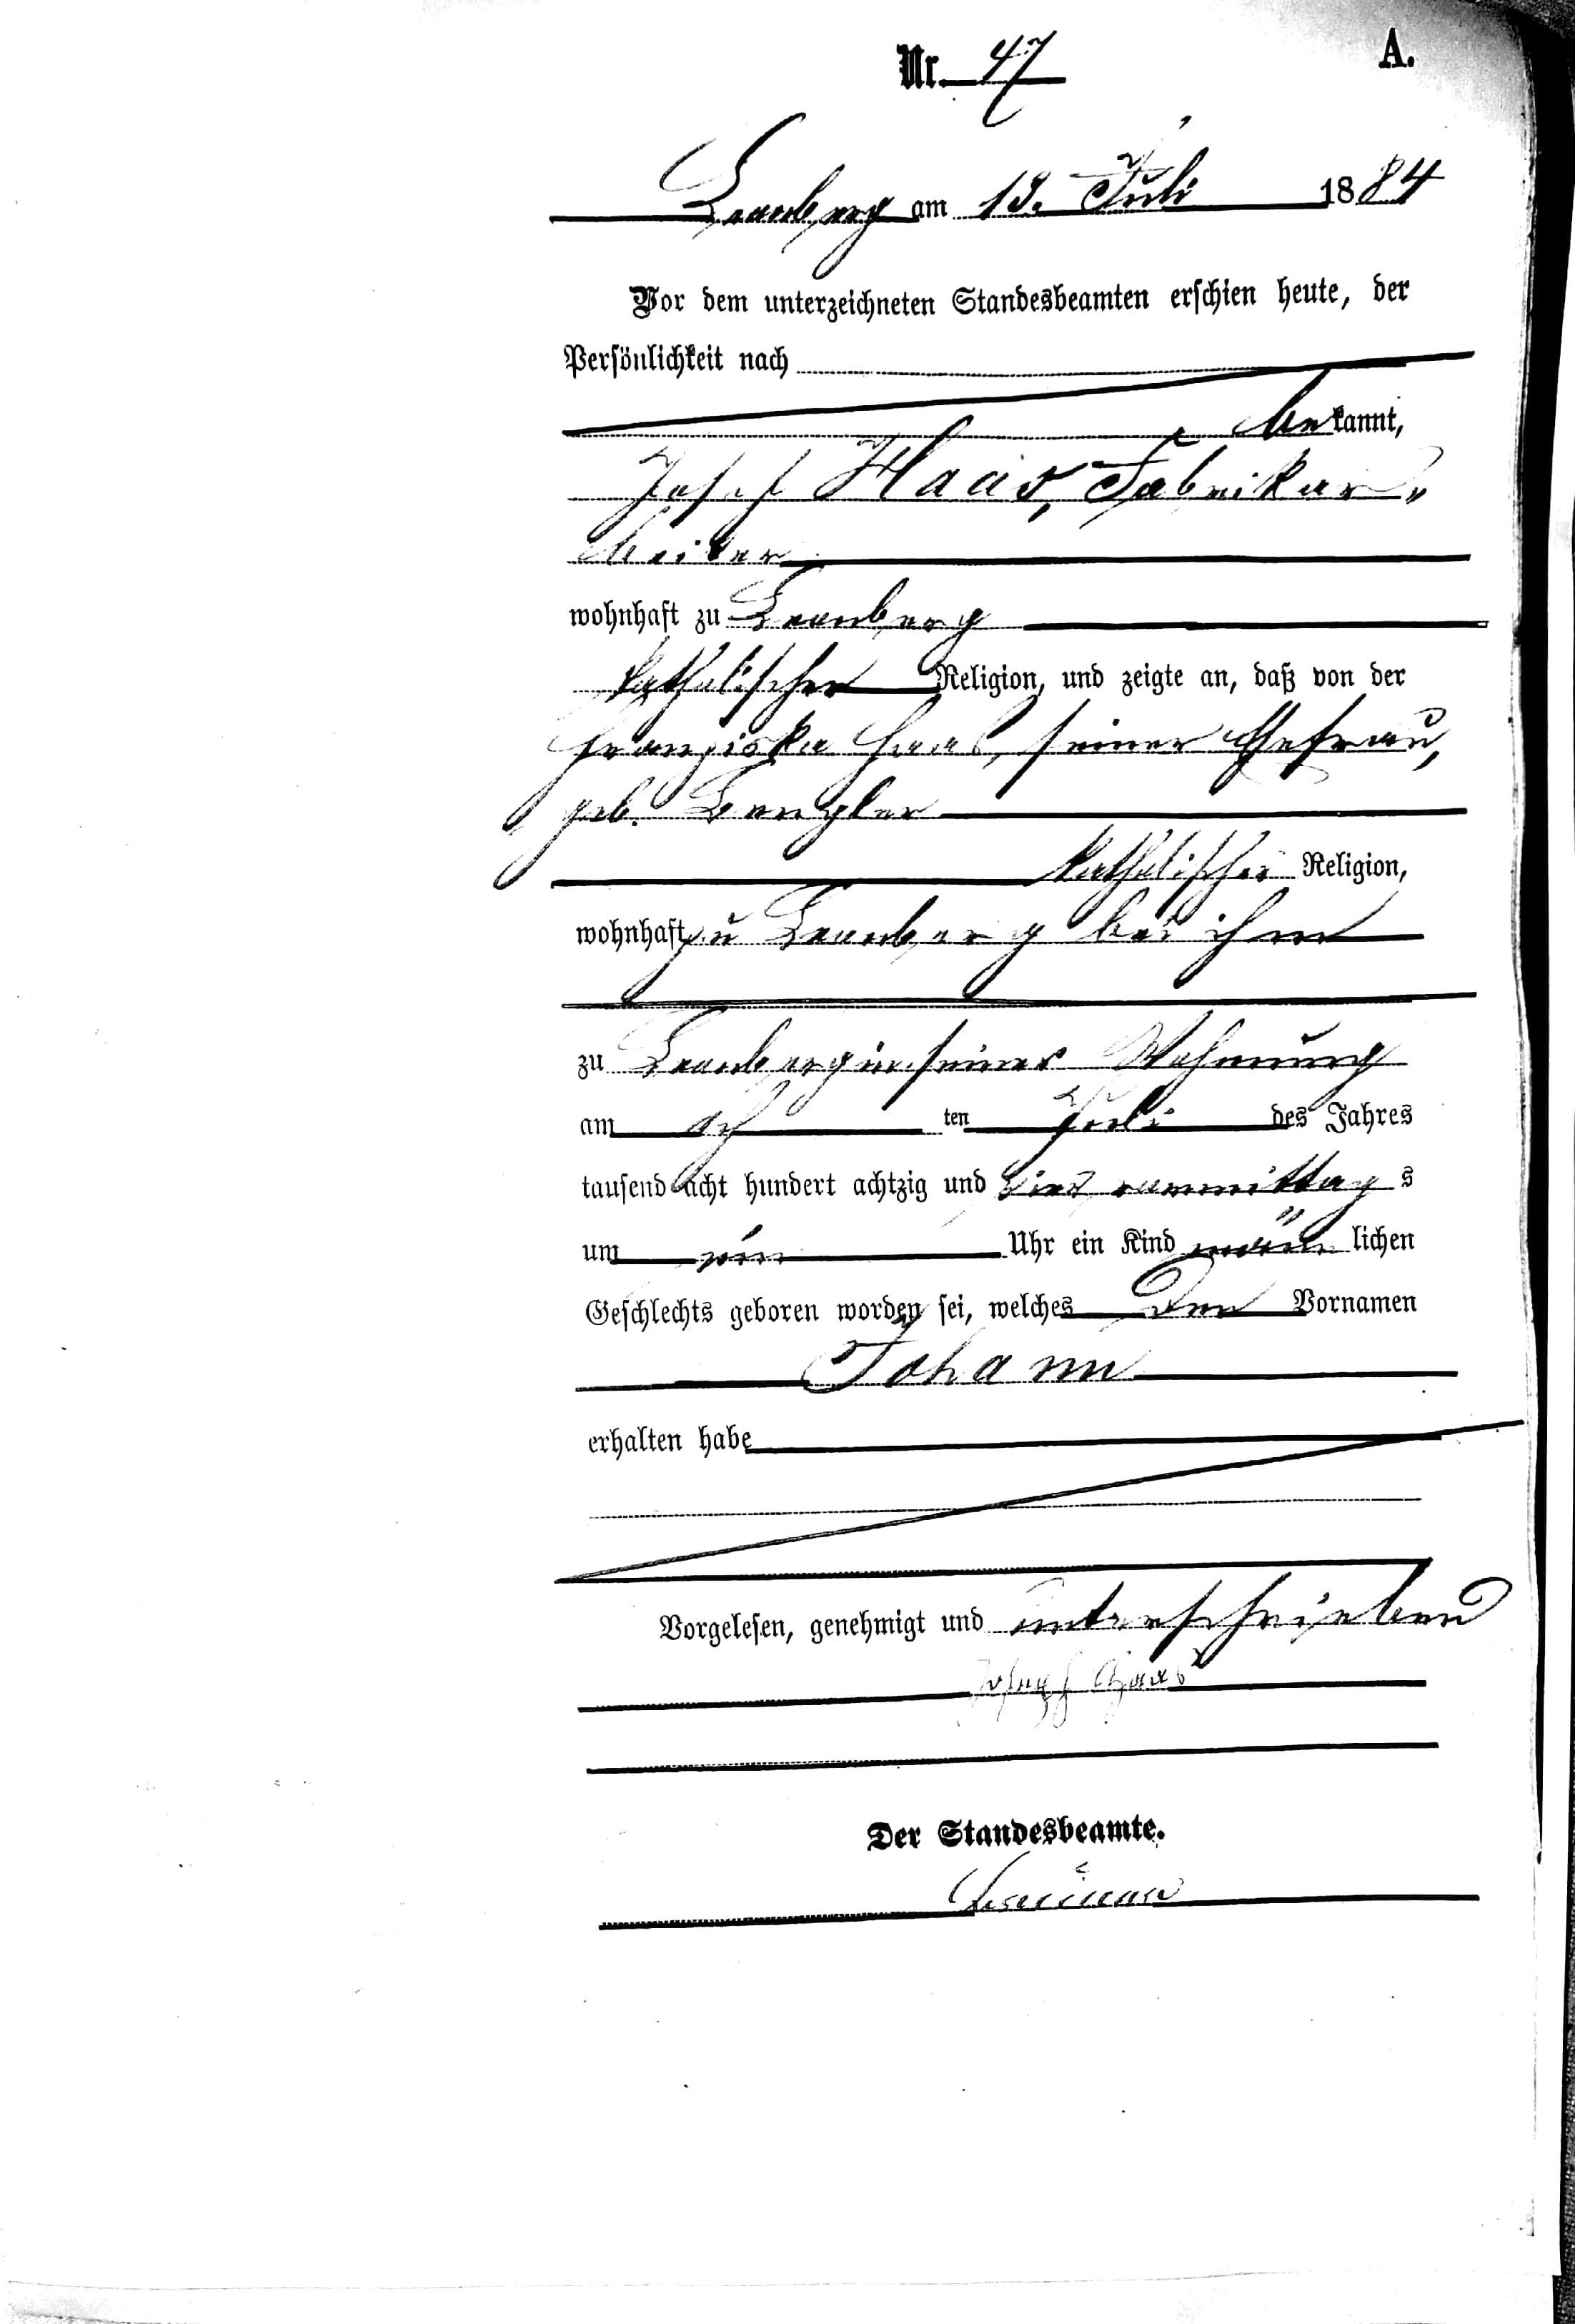
\includegraphics[width=0.85\linewidth,height=\textheight,keepaspectratio,alt={Assento nº 47 do registro civil de Leonberg, de 13 de julho de 1884: o operário Josef Haas declara o nascimento do filho Johann, ocorrido em 11 de julho, às cinco da tarde, e assina o termo com a própria mão.}]{imagens/doc_haas_nascimento_johann_1884.jpg}
\caption{Assento nº 47 do registro civil de Leonberg, de 13 de julho de
1884: o operário Josef Haas declara o nascimento do filho Johann,
ocorrido em 11 de julho, às cinco da tarde, e assina o termo com a
própria mão.}
\end{figure}

Havia uma dúvida que aquele papel resolvia. Na planilha do Agenor, que
foi durante anos a nossa melhor fonte, Johann aparece nascido em ``08 de
julho''. O assento diz onze. A diferença é de três dias e pode parecer
pequena, mas para um pesquisador é tudo: uma das datas está certa e a
outra está errada, e só o documento original decide. O Agenor, que é
engenheiro, sabe melhor do que ninguém que uma medida conferida vale
mais que uma medida anotada; neste livro, prevalece o registro civil, e
o Fata faz aniversário no dia 11. Ele morreu em 1969 sem saber que essa
questão existiria. Imagino que acharia graça.

\section{A assinatura}\label{a-assinatura}

Preciso parar um momento naquela assinatura, porque foi ela que me
desmontou.

Um meteorologista passa a vida lidando com sinais indiretos. Não vemos o
vento: vemos o que ele faz com um anemômetro. Não vemos a frente fria:
vemos o salto da temperatura num gráfico. Quase tudo o que sabemos sobre
a atmosfera vem de rastros. E, durante anos, tudo o que eu sabia sobre
os Haas da Alemanha também eram rastros: o nome numa lista de navio,
preenchida por um escrivão francês; o nome numa planilha, digitado por
um primo; o nome num batismo de Stoffen, escrito por um padre, que nem
era o nosso. Sempre a mão de outro.

A assinatura de Josef Haas era a primeira coisa, naquela pilha toda,
escrita por um Haas da Baviera com a própria mão. Não um registro dele:
um gesto dele. Num dia de julho de 1884, um operário de trinta e sete
anos, com as mãos provavelmente marcadas pelo trabalho na usina, pegou
uma caneta de bico e desenhou o próprio nome numa folha oficial, para
dizer ao Estado que tinha nascido um filho. Esse filho seria o meu avô.
A caneta tremeu um pouco. A tinta borrou numa letra. E o papel guardou
tudo isso por cento e trinta e quatro anos.

Permito-me, aqui, uma cena reconstituída, e vocês sabem que, quando faço
isso, é imaginação apoiada em documento.

\emph{Leonberg, Alto Palatinado, 13 de julho de 1884.} Josef Haas sai de
casa num domingo de verão. Faz dois dias que Franziska deu à luz, às
cinco da tarde de uma sexta-feira, e a lei manda declarar o nascimento
ao oficial. Ele veste, imagino, a roupa menos gasta que tem. O oficial o
conhece; o assento diz \emph{der Persönlichkeit nach bekannt}, conhecido
pessoalmente, o que quer dizer que Josef não precisou de testemunhas
para provar quem era. Leonberg é pequena, e um operário da usina é gente
conhecida. O oficial preenche o formulário, pergunta o nome da criança.
``Johann'', diz Josef. É um nome comum, o mais comum de todos na Baviera
católica, o nome do Batista e do Evangelista. O oficial escreve. Lê o
termo em voz alta. Josef diz que está certo e assina.

Não sei se foi assim. Sei que poderia ter sido, e que o essencial está
no papel: o dia, a hora, os nomes, a assinatura.

Penso, olhando aquela letra, em todos os papéis que Johann assinaria
depois. O casamento em Eibenstock, em 1907. Algum documento de embarque
em Marselha, em 1913. A escritura do Lote 17 em Rio do Ouro, com o amigo
com quem comprou a terra. Os contratos das obras de Ituporanga: a Igreja
Matriz, a Casa Paroquial, o Seminário Franciscano, a ampliação do
Hospital das Irmãs. Nenhum desses papéis está comigo. Mas eu sabia, de
repente, como a letra do pai dele tinha sido. E pensei na minha própria
assinatura, que vocês conhecem dos boletins da escola, das autorizações
de passeio, das procurações. Está tudo ligado por uma mesma mão que vai
mudando de dono.

\section{A segunda folha}\label{a-segunda-folha}

O registro de Johann era o que eu tinha ido buscar. A segunda folha foi
o que eu encontrei.

Nas buscas que se fazem num cartório municipal alemão, o sistema da
prefeitura consulta os registros pelo sobrenome. E, entre os resultados
daquela manhã, apareceu uma pessoa viva: um Haas, nascido em Leonberg em
1941, residente em Maxhütte-Haidhof.

Vou ser cuidadoso aqui, e explico por quê. Esse homem existe: é uma
pessoa de carne e osso que, quando estive lá, tinha setenta e poucos
anos, morava na mesma cidade onde o Fata nasceu e não sabia (ou, se
sabia, não sabia de mim) que um descendente do filho emigrado de Josef
Haas estava na mesma cidade segurando uma árvore genealógica. Ele tem
direito à sua privacidade, e a lei europeia, além do bom senso, protege
esse direito. Por isso este livro não traz o nome dele, nem a rua, nem
nada que permita encontrá-lo. E este livro não conta um encontro com
ele. Contaria, se houvesse para contar.

Um Haas nascido em Leonberg em 1941. Durante a guerra. No mesmo ano em
que, do outro lado do mundo, o Brasil rompia com a Alemanha e, no Alto
Vale do Itajaí, o Fata guardava a espingarda carregada ao alcance da mão
e ouvia o rádio no porão, com um neto vigiando a estrada. Enquanto a
família de Santa Catarina aprendia a ter medo de falar alemão, nascia em
Leonberg uma criança com o mesmo sobrenome, numa Alemanha que ia ser
bombardeada, ocupada, dividida. As duas metades da família viveram a
mesma guerra de lados opostos do oceano e sem saber uma da outra. O
texto do centenário diz que, em 1945, João e Maria mandaram roupas e
mantimentos para a Alemanha arrasada sem saber se ainda tinham parentes
vivos lá, ``se é que ainda os tinham''. Talvez tivessem: em Leonberg
havia um menino de quatro anos com o mesmo sobrenome.

Não sei que parentesco ele tem conosco. Johann tinha irmãos: Josef,
Alois, Georg, Maria, Franziska, Therese. Os homens transmitiram o
sobrenome. Se esse Haas de 1941 for neto de um deles, então ele é primo
em segundo grau do meu pai, o vô Baldoíno. Primo de terceiro grau meu. E
de vocês, primo ainda mais distante, mas primo. Pode também não ser nada
disso. Haas não é um sobrenome raro na Alemanha, e um homônimo numa
cidade de operários seria perfeitamente possível. Um pesquisador honesto
não pode afirmar o parentesco sem documento, e eu não tenho o documento.
Tenho a coincidência de lugar, que é forte, e a coincidência de nome,
que é fraca.

Há ainda a armadilha dos homônimos, de que falei no capítulo 2. Existe
um Leonberg muito mais famoso que o nosso, perto de Stuttgart, em
Württemberg, e existe um Heumaden também por lá, hoje bairro de
Stuttgart. Durante muito tempo, quem procurava os nossos nomes nos mapas
caía primeiro nesses lugares, a centenas de quilômetros do lugar certo.
Um meteorologista conhece esse tipo de erro: é o de uma estação com as
coordenadas trocadas, que manda um dado correto do lugar errado e
contamina o mapa inteiro. Por isso, um sobrenome igual numa cidade de
nome igual não me basta. Mas aqui não há confusão possível de lugar: era
o Leonberg do assento nº 47, o Leonberg do Alto Palatinado, o mesmo onde
Josef assinou em 1884. Se há ambiguidade, ela está só no sangue.

Há uma complicação, e a registro porque ela é parte da história. Na
mesma viagem, procurei a casa. Peter, com quem conversei, disse que o
primo do meu pai estava vivo. Os vizinhos da casa a que cheguei disseram
outra coisa: que o Haas de mesmo nome tinha morrido e que as filhas dele
moravam na Áustria. Talvez eu tenha batido na casa errada. Talvez os
dois estivessem falando de pessoas diferentes. Não resolvi isso lá, e
não vou resolver aqui com palpites.

E há um silêncio que agora entendo de outro modo. O Fata não falava dos
parentes vivos da Alemanha. Mas a família guardou cartas vindas de lá,
de um endereço no Vogtland, na Saxônia. Alguém, do outro lado, sabia de
nós.

Naquela manhã, eu não pensei como pesquisador. Pensei como neto. O que
senti foi o que imagino que sente um náufrago que, depois de muitos
dias, vê fumaça numa ilha. Não é o resgate. É a prova de que há gente.

Durante toda a pesquisa, desde a mesa de Vidal Ramos em 2012, a pergunta
que movia este livro era essa: \emph{ainda há alguém do outro lado?} O
Fata morreu em 1969 achando que não. Eu achava que a Mota tinha morrido
em 1973 sem que ninguém do outro lado soubesse. Só em 2026, com as
cartas de Rempesgrün do Capítulo 7, descobri que os parentes dela, na
Saxônia, souberam e mandaram pêsames. Quem tinha deixado o fio cair
éramos nós. E ali estava, numa tela de computador de uma prefeitura do
Alto Palatinado, a ponta do fio do outro lado.

Escrevo estas páginas, então, também como uma carta possível. Se um dia
este livro chegar, traduzido ou não, a um Haas nascido em Leonberg em
1941, quero que ele saiba que em 1913 um rapaz chamado Johann, filho do
operário Josef e de Franziska Dengler, saiu dali e partiu com a mulher e
dois filhos pequenos para o Brasil; que esse rapaz construiu igrejas e
túmulos num lugar chamado Ituporanga; que teve doze filhos, dos quais
sete chegaram à idade adulta; que hoje os descendentes dele são mais de
seiscentos; e que um desses descendentes esteve na Regensburger Straße
numa manhã de fevereiro e soube que ele existia. A porta fica aberta.
Não sei se alguém vai bater.

\section{O balão atravessa a nuvem}\label{o-baluxe3o-atravessa-a-nuvem}

Há um momento, na vida de um meteorologista, que nunca deixa de ser
bonito: o lançamento de uma radiossonda. Um balão de látex cheio de
hidrogênio ou hélio, com uma pequena caixa de sensores pendurada, sobe
da estação e começa a transmitir pressão, temperatura, umidade. Na tela,
o perfil vai se desenhando de baixo para cima. Durante um tempo, os
números são previsíveis: a temperatura cai, a umidade oscila. E então,
de repente, o balão entra numa nuvem, e a umidade vai a cem por cento, e
a temperatura faz uma curva, e você sabe que ele está lá dentro, no meio
do branco, sem ver nada. E então, mais de repente ainda, ele sai pelo
topo, e a umidade despenca, e o ar fica seco e limpo, e o balão continua
subindo num céu que, de baixo, ninguém via.

Toda a pesquisa, desde 2012, tinha sido o balão dentro da nuvem. Nomes
desencontrados, datas divergentes, lugares homônimos, uma planilha com
lacunas, um manifesto com uma idade errada, um ``Leonberg'' que podia
ser outro Leonberg, um ``Sandberg'' que eu não achava no mapa. Umidade a
cem por cento. E o assento nº 47 foi o momento em que o balão saiu pelo
topo. De uma hora para outra, o ar ficou limpo. Johann Haas, nascido em
11 de julho de 1884, às cinco da tarde, em Leonberg. Filho de Josef
Haas, operário, e de Franziska Dengler. Neto, pelo pai, de Michael Haas
e de Kunigunde Stadelmann, como eu só fui saber em 2026. Uma linha reta,
sem nuvem, de vocês até a fumaça de Sandberg.

Não sei quanto tempo ficamos lá dentro. Não vou inventar. Sei que saí
com o papel e que, na rua, o frio era o mesmo de antes, mas eu não era.

Hoje, quando volto àquela manhã, penso no vô Baldoíno, que morreu em
dezembro de 2013, quatro anos antes dela. Ele era o décimo filho de
Johann, o que nasceu na clareira de Rio Novo em 1924. Ele teria gostado
de ver aquele papel. Talvez não dissesse nada, porque os homens da
geração dele diziam pouco. Talvez só passasse o dedo devagar sobre a
assinatura do avô que nunca conheceu. Penso na vó Adelina, viva ainda
naquele fevereiro, em Vidal Ramos. Penso em vocês dois, que um dia
leriam isto.

E penso, finalmente, no que aquele papel ainda não dizia: faltava
metade. O assento nº 47 me dava o Fata inteiro, com pai, mãe, avô e
aldeia. Mas o Fata nunca foi sozinho. Ao lado dele, no manifesto, na
fotografia de despedida, no túmulo de Aurora, havia sempre ela. A moça
que nasceu às duas da madrugada numa aldeia de colinas perto da Boêmia,
cujo nome a família repetiu por um século como quem repete uma oração
sem entender o sentido das palavras.

Faltava a outra metade: a Mota. Faltava Heumaden.

\section{Para vocês descobrirem}\label{para-vocuxeas-descobrirem-16}

\begin{itemize}
\tightlist
\item
  Que parentesco, se é que há algum, liga o Haas nascido em Leonberg em
  1941 a Josef Haas? Se ele for neto de um irmão de Johann, de qual:
  Josef, Alois ou Georg?
\item
  Quem tinha razão: Peter, que disse que o primo do meu pai estava vivo,
  ou os vizinhos, que disseram que o Haas de mesmo nome tinha morrido e
  que as filhas dele moravam na Áustria? Bati na casa errada?
\item
  Quem, do outro lado, escreveu as cartas do Vogtland, e o que elas
  dizem? Perguntem aos mais velhos da família onde essas cartas estão.
\item
  De quem Johann aprendeu o gesso, se o texto do centenário diz que ele
  ``vinha de uma família de pedreiros'' e o pai era operário de usina?
  Dos Dengler, dos irmãos mais velhos de Josef, ou de ninguém da
  família?
\end{itemize}

\chapter{A Estrada para Heumaden e a Letra Gótica de
Moosbach}\label{cap-18}

\emph{49,6° N · 12,4° E, Moosbach, Alto Palatinado (Heumaden,
Rückersrieth, Burgtreswitz)}

\begin{quote}
\emph{A tinta de um padre de aldeia dura mais que a aldeia que ele
conheceu.}
\end{quote}

Uma página de um livro paroquial bávaro, tal como a leio, contradiz o
que a família anotou sobre o batismo da Mota: o dia e o nome da
madrinha. Outra traz um sobrenome que parece ter sido retocado. Este
capítulo é sobre quatro páginas.

\section{Uma estrada que primeiro se percorre no
mapa}\label{uma-estrada-que-primeiro-se-percorre-no-mapa}

Heumaden fica a uns cinquenta quilômetros de Maxhütte-Haidhof em linha
reta, na direção nordeste, quase na mesma longitude, um pouco mais perto
da fronteira tcheca. É uma dessas aldeias que, no mapa, cabem numa
vírgula: um punhado de telhados, uma estrada vicinal, campos em volta,
manchas escuras de floresta. Faz parte hoje do município de Moosbach, no
distrito de Neustadt an der Waldnaab, no Alto Palatinado. A paróquia é a
de São Pedro e São Paulo (\emph{St.~Peter und Paul}), no centro de
Moosbach, que os alemães chamam de \emph{Markt}, uma vila com direito
antigo de feira. Em volta, a poucos quilômetros uns dos outros, estão os
outros nomes desta história: Rückersrieth, onde nasceu o bisavô Georg
Adam Meier; Burgtreswitz, onde nasceu a bisavó Franziska Voit, uma
aldeia que leva no nome a palavra \emph{Burg}, castelo, porque tem um.

A primeira vez que percorri essa estrada foi no mapa, e é assim que
quero começar, porque é assim que vocês provavelmente a percorrerão
também. Abri a imagem de satélite e fui aproximando. Primeiro a Europa,
depois a Alemanha, depois a Baviera, depois aquela região de colinas
baixas e florestas entre o Danúbio e a Boêmia que os alemães chamam de
\emph{Oberpfälzer Wald}, a Floresta do Alto Palatinado. Depois Moosbach,
com sua igreja. Depois, a nordeste, Heumaden. Algumas casas, uma rua,
campos repartidos em faixas compridas, a herança antiga da lavoura
medieval. Fiquei olhando aquelas faixas por muito tempo. Numa delas,
talvez, a Mota tenha ordenhado vacas quando moça, antes de casar e ir
embora. O texto do centenário diz que Maria ``recebia salário ordenhando
vacas''. Era ela, diz Marise, ``quem conhecia a lida do campo''.

O próprio nome da aldeia parece falar de campo. \emph{Heu} é feno;
\emph{Mahd} é a ceifa, o corte da relva com a foice. Não sou filólogo e
não vou jurar pela etimologia, mas é difícil não ouvir em
\emph{Heumaden} algo como ``os prados de feno'', ``o lugar onde se
ceifa''. Uma aldeia de pasto e de vacas. Faz sentido que a Mota tenha
crescido ordenhando. E faz sentido, de um jeito que só percebi depois,
que ela tenha passado a velhice em Ribeirão das Pacas, no Alto Vale do
Itajaí, cuidando de bichos e de roças, apoiada nas bengalas de pau de
que os netos se lembram. O texto de Marise diz que, perto da filha
Maria, ela continuou ``revolvendo o chão, cultivando suas plantas e
criando seus animais''.

Para um meteorologista, aquela região tem ainda outra marca: é o lado de
dentro do continente. Longe do mar, o Alto Palatinado tem invernos mais
frios e verões mais quentes que o oeste da Alemanha, e o vento que vem
do leste, da Boêmia, chega seco e cortante. Os moradores antigos tinham
nome para ele. A Mota cresceu sob esse clima de amplitude grande, de
geada longa e verão curto, e foi parar num lugar onde a umidade nunca
baixa e o inverno é uma estação de poucas semanas. Não sei o que o corpo
dela achou da troca. Sei que viveu oitenta e cinco anos.

Os livros paroquiais de Moosbach são guardados hoje pelo arquivo central
da diocese de Regensburg, o \emph{Bischöfliches Zentralarchiv}, e foram
digitalizados e postos ao alcance de qualquer pessoa no portal
Matricula, que reúne registros de igrejas de meia Europa. É por essas
imagens digitais que cito as páginas (o livro de batismos de 1847 a
1904, o livro de casamentos de 1853 a 1935), porque é por elas que
vocês, ou qualquer primo, poderão conferir cada linha que vou
transcrever. Seja qual for a sala, a mesa ou a tela diante da qual se
abre um livro desses, a experiência é a mesma: uma página antiga, uma
letra que não se entende e a esperança de achar, no meio dela, um nome
conhecido.

\section{A letra que a Mota sabia
ler}\label{a-letra-que-a-mota-sabia-ler}

A primeira coisa que um brasileiro descobre diante de um livro paroquial
bávaro do século XIX é que não sabe ler.

O problema é a letra. Os padres e escrivães daquela época escreviam em
\emph{Kurrentschrift}, a escrita cursiva alemã, que foi a letra comum
dos países de língua alemã durante séculos, até ser abandonada em meados
do século XX. Ela não se parece com nada que aprendemos na escola. O
``e'' é feito com dois traços verticais quase iguais, como um ``n''
apertado. O ``h'' desce abaixo da linha como uma cauda. O ``s'' tem duas
formas, uma comprida no meio das palavras e outra redonda no fim. O
``r'' parece um ``w'' pequeno. O ``M'' maiúsculo, que eu precisava achar
acima de tudo, porque era a inicial de Meier, é uma sequência de arcos
que, à primeira vista, poderia ser qualquer coisa.

A Mota sabia ler essa letra. O Fata também. Eles aprenderam a escrever
assim nas escolas da Baviera, e o texto do centenário conta que eram
leitores, que trouxeram livros da Alemanha e depois assinavam jornais de
Blumenau, que no começo do século XX ainda se imprimiam em letra gótica.
Os filhos deles, nascidos no Brasil, foram à escola falando só alemão,
mas aprenderam a escrever no alfabeto latino, em português. Eu, o neto,
precisei de tabelas, de exemplos, de muita paciência para reconhecer o
nome da minha avó numa página escrita na letra que ela própria usava
para escrever cartas. É uma das formas mais concretas da língua
silenciada de que falei no capítulo 7: perdeu-se a fala e perdeu-se a
mão.

Aprendi devagar. Primeiro as letras isoladas, depois as abreviações. Os
padres abreviavam tudo: \emph{Gg.} para Georg, \emph{Kath.} para
Katharina, \emph{Mich.} para Michael, \emph{Joh.} para Johann, \emph{k.}
ou \emph{kath.} para católico. Usavam aspas como sinal de ``idem'',
repetindo o que estava na linha de cima. Misturavam o latim no alemão:
\emph{et} para ``e'', \emph{Procl.} para as proclamações canônicas,
\emph{idem} para o mesmo padre. E escreviam os números de um jeito que
um meteorologista, acostumado a ler planilhas, achou quase familiar.

Os livros de batismo de Moosbach são tabelas. Cada linha é uma criança.
As colunas, da esquerda para a direita, trazem o número do registro, o
nome da criança, a parteira, o pai e sua condição, o lugar de moradia, a
mãe e sua condição, a origem da mãe, o dia e a hora do nascimento, o dia
do batismo, o padre, os padrinhos. Cada página dupla tem uns poucos
registros, e cada ano, algumas dezenas. Para achar Maria Meier, eu sabia
o ano e o mês. Abril de 1888. Era só uma questão de virar páginas até
lá.

\section{Página 441, registro nº
36}\label{puxe1gina-441-registro-nuxba-36}

Lá estava.

Na página 441 do livro de batismos, entre uma menina chamada Josefa, de
uma família de Moosbach, nascida no dia anterior, e um menino de
sobrenome Bergmann, nascido no mesmo dia que ela: o registro número 36.
Na coluna do nome, em duas linhas, o sobrenome primeiro, como se fazia:
\emph{Meier}, depois \emph{Maria}.

Vou ler a linha com vocês, coluna por coluna, como a li.

Parteira: duas aspinhas. \emph{Idem}. Para saber quem era, é preciso
subir uma linha, até o registro 35, o da pequena Josefa, nascida no dia
6 de abril à uma da madrugada. Ali está o nome: \emph{Glas}. A senhora
Glas, parteira de Moosbach, tinha feito um parto na madrugada de 6 de
abril e outro na madrugada de 7. Duas noites seguidas atravessando o
frio da primavera bávara com a sua maleta. Quando, no capítulo 4,
imaginei a noite do nascimento da Mota, eu ainda não tinha reparado nas
duas aspinhas. Agora sei que a senhora Glas, naquela madrugada,
provavelmente estava cansada.

Pai: \emph{Gg. Adam Meier}. Condição, na leitura que fizemos e que
confere com as transcrições do dossiê: \emph{Ökonom}, que na Baviera
daquela época queria dizer agricultor. Morada: \emph{Heumaden}. Mãe:
\emph{Franzisca Voit}. Origem da mãe: \emph{Burgtresw.}, Burgtreswitz.

Nascimento: \emph{7. April, 2 h. morg.} (7 de abril, duas horas da
manhã).

Batismo: \emph{7. April}.

Madrinha: \emph{Kath. Reichenberger, Bäuerin v. Burgtresw.} (Katharina
Reichenberger, lavradora de Burgtreswitz).

\begin{ficha}

\textbf{Ficha do Arquivo}: Paróquia de St.~Peter und Paul, Moosbach
(Decanato de Leuchtenberg, Diocese de Regensburg). Livro de batismos
1847--1904 (Matricula: \texttt{Moosbach\_Leuchtenberg005}), p.~441,
registro nº 36. Batizada: Maria Meier. Parteira: Glas (indicada por
``idem'', remetendo ao registro anterior). Pai: Georg Adam Meier
(\emph{Gg. Adam Meier}), \emph{Ökonom} em Heumaden. Mãe: Franziska Voit
(\emph{Franzisca Voit}), natural de Burgtreswitz. Nascimento: 7 de abril
de 1888, às 2 horas da manhã, em Heumaden. Batismo: 7 de abril (data
registrada na coluna própria, segundo a nossa leitura). Madrinha:
\emph{Kath. Reichenberger, Bäuerin v. Burgtresw.} Imagem:
\texttt{imagens/doc1\_maria\_meier\_1888.jpg}.

\end{ficha}

\begin{figure}
\centering
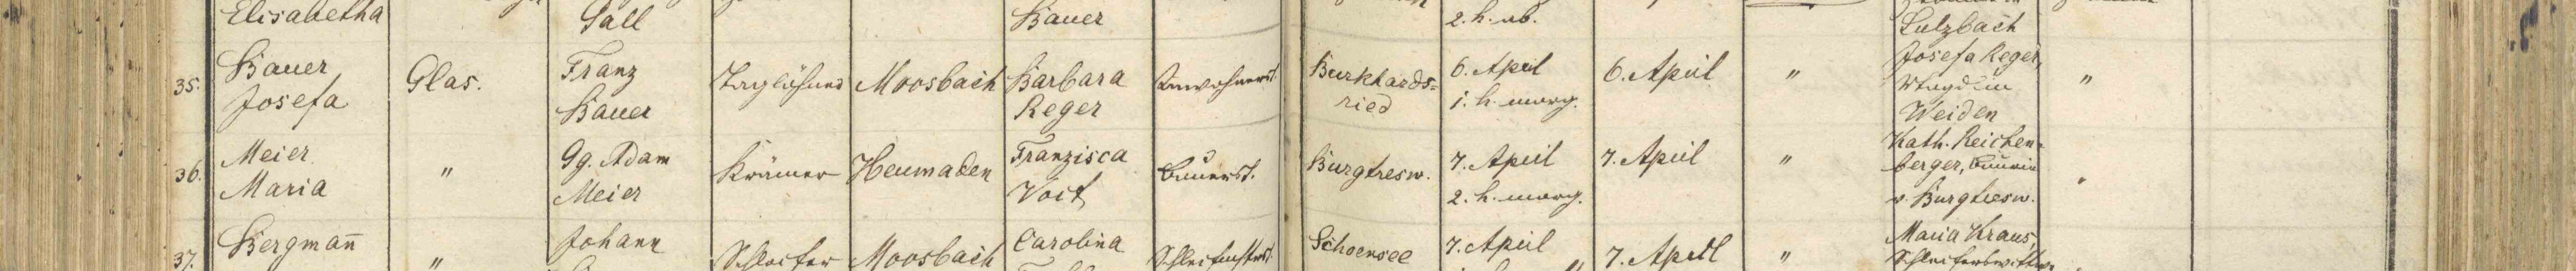
\includegraphics[width=0.85\linewidth,height=\textheight,keepaspectratio,alt={Livro de batismos de Moosbach, página 441: o registro nº 36, de Maria Meier, nascida em Heumaden em 7 de abril de 1888, às duas da madrugada, filha de Georg Adam Meier e Franziska Voit; na linha de cima, o nome da parteira Glas.}]{imagens/doc1_maria_meier_1888.jpg}
\caption{Livro de batismos de Moosbach, página 441: o registro nº 36, de
Maria Meier, nascida em Heumaden em 7 de abril de 1888, às duas da
madrugada, filha de Georg Adam Meier e Franziska Voit; na linha de cima,
o nome da parteira Glas.}
\end{figure}

Preciso contar uma coisa, porque este livro tem uma regra e eu não vou
quebrá-la logo no capítulo em que ela mais importa.

Nas anotações que circulavam na família, e que eu mesmo repeti em mais
de um lugar, Maria foi batizada no dia 8 de abril, e a madrinha foi a
tia dela, Katharina Meier, lavradora de Heumaden. A página 441, tal como
a leio, diz outra coisa. A coluna do batismo traz ``7. April'', o mesmo
dia do nascimento, o que era muito comum na Baviera católica, onde se
batizava depressa por medo de que a criança morresse pagã. E a madrinha
se chama Katharina Reichenberger, de Burgtreswitz, a aldeia da mãe.

Há uma hipótese que concilia as duas versões, e eu a registro como
hipótese: uma Katharina nascida Meier, irmã de Georg Adam, poderia estar
casada com um Reichenberger de Burgtreswitz; nesse caso, seria ao mesmo
tempo ``a tia Katharina'' da tradição e a ``Kath. Reichenberger'' do
livro. Seria bonito. Mas não tenho o documento que prove isso, e uma
hipótese bonita é exatamente o tipo de coisa de que um pesquisador deve
desconfiar mais. Deixo as duas versões lado a lado, como deixei, nos
capítulos anteriores, as duas datas de Gertrudes e os dois lugares de
sepultura de Luisa e Walter. A verdade sobre a madrinha da Mota está em
algum outro livro, num registro de casamento de Burgtreswitz que ainda
não li. Fica para vocês, se quiserem.

Nenhuma dessas dúvidas tira o essencial. Em 7 de abril de 1888, às duas
da madrugada, numa casa de Heumaden, nasceu a menina que seria a Mota. O
nome que a família repetiu por um século em Ituporanga e em Aurora, sem
que ninguém soubesse exatamente onde ficava, tinha uma linha num livro.

Permito-me, outra vez, imaginar.

\emph{Moosbach, Alto Palatinado, 7 de abril de 1888.} É um sábado. A
senhora Glas deixou a casa dos Meier ainda de madrugada. Mais tarde,
alguém leva a recém-nascida até a igreja de São Pedro e São Paulo,
enrolada em panos contra o frio de abril. É provável que a mãe,
Franziska, não vá; as mulheres que acabavam de dar à luz ficavam em
casa. Vão o pai, a madrinha, talvez uma vizinha. O padre derrama a água,
diz o nome. Depois, na sacristia, abre o livro grande e escreve, na
letra que eu levaria um século para aprender a ler, a linha número 36
daquele ano. Ninguém ali imagina que essa menina vai morrer do outro
lado do mundo, aos 85 anos, numa terra chamada Aurora, sem nunca mais
ver aquela igreja.

\section{Vinte e três de novembro de
1884}\label{vinte-e-truxeas-de-novembro-de-1884}

Com Maria encontrada, o resto do quebra-cabeça veio por gravidade. Se
ela era filha de Georg Adam Meier e Franziska Voit, os dois tinham
casado ali, alguns anos antes. O livro de casamentos de Moosbach, que
vai de 1853 a 1935, tem na página 93 o registro número 20.

A data, na primeira coluna: \emph{23. Nov.}, 23 de novembro de 1884. Um
domingo.

Noivo: \emph{Adam Meier}. Condição: \emph{Wagner}, católico.
\emph{Wagner}, em alemão, é o fabricante de rodas e carroças, o
carpinteiro especializado que fazia os aros, os raios, os cubos, as
carroças inteiras com que se trabalhava o campo. Morada: Heumaden. Pais:
\emph{Mich. Meier et Margaretha Pfanenstein}, com um ``n'' só e um
tracinho em cima, que é como se abreviava a letra dobrada. Estado:
solteiro. Nascido em: \emph{9. März 1859}.

Noiva: \emph{Franzisca Voit}. Condição: \emph{Bauerstochter}, filha de
lavrador, católica. Morada: Burgtreswitz. Pais: \emph{Joh. Voit et
Barbara Woppman}. Estado: solteira. Nascida em: \emph{29. Juni 1861}.

Testemunhas: \emph{Mich. Meier, Wagner, Heumaden, et Johan Voit, Bauer,
Burgtreswitz}. Os dois pais. O pai do noivo, que fazia rodas, e o pai da
noiva, que lavrava a terra, de pé ao lado dos filhos diante do altar.

Depois, a data da licença civil, \emph{8. Nov.~1884}, porque desde 1876
também o casamento precisava passar pelo registro civil, e as \emph{3
Procl.}, as três proclamações canônicas, os anúncios feitos na missa em
três domingos seguidos para que, se alguém soubesse de algum
impedimento, falasse. Ninguém falou.

\begin{ficha}

\textbf{Ficha do Arquivo}: Paróquia de St.~Peter und Paul, Moosbach.
Livro de casamentos 1853--1935 (Matricula:
\texttt{Moosbach\_Leuchtenberg013}), p.~93, registro nº 20. Data: 23 de
novembro de 1884. Noivo: Adam (Georg Adam) Meier, \emph{Wagner},
católico, de Heumaden, filho de Michael Meier e Margaretha Pfannenstein
(\emph{Pfanenstein}), solteiro, nascido em 9 de março de 1859. Noiva:
Franziska Voit (\emph{Franzisca}), \emph{Bauerstochter}, católica, de
Burgtreswitz, filha de Johann Voit e Barbara Woppmann (\emph{Woppman}),
solteira, nascida em 29 de junho de 1861. Testemunhas: Michael Meier,
\emph{Wagner} em Heumaden, e Johann Voit, \emph{Bauer} em Burgtreswitz.
Licença civil: 8 de novembro de 1884. Três proclamações. Imagem:
\texttt{imagens/doc2\_trauung\_meier\_voit\_1884.jpg}.

\end{ficha}

\begin{figure}
\centering
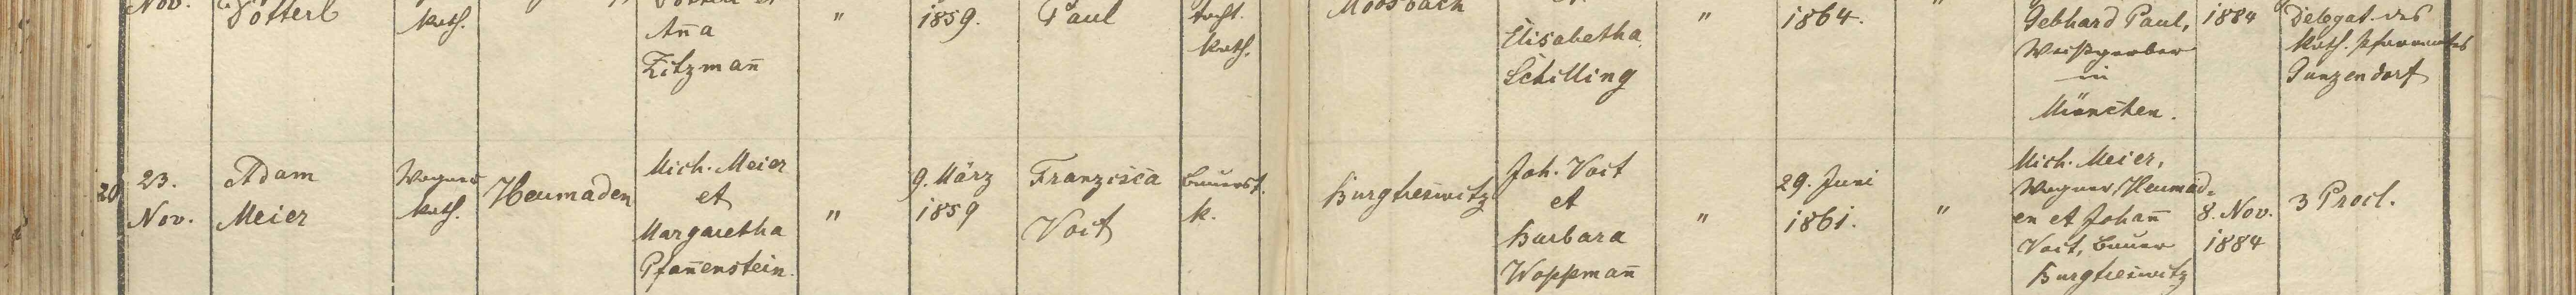
\includegraphics[width=0.85\linewidth,height=\textheight,keepaspectratio,alt={Livro de casamentos de Moosbach, página 93: o registro nº 20, do casamento de Adam Meier, fabricante de rodas de Heumaden, com Franziska Voit, filha de lavrador de Burgtreswitz, em 23 de novembro de 1884, tendo os dois pais por testemunhas.}]{imagens/doc2_trauung_meier_voit_1884.jpg}
\caption{Livro de casamentos de Moosbach, página 93: o registro nº 20,
do casamento de Adam Meier, fabricante de rodas de Heumaden, com
Franziska Voit, filha de lavrador de Burgtreswitz, em 23 de novembro de
1884, tendo os dois pais por testemunhas.}
\end{figure}

Fiz a conta que todo genealogista acaba fazendo. Em 23 de novembro de
1884, enquanto Adam e Franziska casavam em Moosbach, um bebê de quatro
meses chamado Johann Haas dormia em Leonberg, a cinquenta quilômetros
dali. Os pais do Fata e os pais da Mota não se conheciam, provavelmente
nunca se conheceram, e, no entanto, naquele outono, as duas linhas já
estavam traçadas no mapa.

Notei também a mudança de ofício. Em 1884, Adam é \emph{Wagner}, como o
pai. Em 1888, no batismo de Maria, é \emph{Ökonom}. Entre um registro e
outro, o fabricante de rodas parece ter passado a viver da terra, talvez
a da família da mulher, talvez a que comprou ou herdou. Não sei os
detalhes. O filho do \emph{Wagner} virou lavrador. A filha do lavrador,
Maria, ordenharia vacas por salário. E o neto dela seria pedreiro em
Santa Catarina.

\section{Dois batismos, um de inverno e um de
verão}\label{dois-batismos-um-de-inverno-e-um-de-veruxe3o}

Faltavam os dois do altar. Voltei ao livro de batismos, agora para trás.

O primeiro está na página 96, no ano de 1859. A linha é de uma
quarta-feira de março. Nome: \emph{Adam}, e depois \emph{Meier}. Aqui o
registro tem uma particularidade que demorei a entender. O sobrenome
parece ter sido retocado, como se outra coisa estivesse escrita antes e
tivesse sido corrigida. A transcrição do dossiê que reúne esses
documentos interpreta o detalhe como uma legitimação: Adam teria nascido
antes do casamento dos pais e sido reconhecido depois, quando Michael e
Margaretha casaram. Não sou paleógrafo para afirmar isso com certeza, e
por isso digo apenas o que vejo: um nome que foi mexido. Se a leitura do
dossiê estiver certa, o bisavô de vocês, Georg Adam, começou a vida com
uma pequena irregularidade que o tempo e o casamento dos pais trataram
de corrigir.

O pai: \emph{Michael Meier}, \emph{Wagner}, de Heumaden. A mãe:
\emph{Margaretha Pfannenstein}, filha de lavrador. O lugar associado ao
nascimento: \emph{Rückersrieth}, a aldeia dela. Nascimento: \emph{9.
März, 3 Uhr früh} (9 de março, três da madrugada). Batismo: \emph{9.
März in Moosbach}, no mesmo dia. Padre: \emph{idem}. E o padrinho:
\emph{Adam Hartung}, filho do ferreiro de Heumaden.

Foi ali que entendi de onde vinha o nome. Na Baviera, era comum que a
criança recebesse o nome do padrinho. Georg Adam Meier se chamou Adam
por causa de Adam Hartung, filho do ferreiro. Um filho de fabricante de
rodas batizado com o nome de um filho de ferreiro. Na aldeia, o ferreiro
e o \emph{Wagner} trabalhavam juntos: um fazia a roda de madeira, o
outro forjava o aro de ferro que a envolvia. A roda inteira dependia dos
dois. Achei aquilo bonito demais para ser só acaso, e talvez não fosse.

\begin{ficha}

\textbf{Ficha do Arquivo}: Paróquia de St.~Peter und Paul, Moosbach.
Livro de batismos 1847--1904 (\texttt{Moosbach\_Leuchtenberg005}),
p.~96. Batizado: Adam (Georg Adam) Meier. Pai: Michael Meier,
\emph{Wagner} em Heumaden. Mãe: Margaretha Pfannenstein,
\emph{Bauerstochter}, de Rückersrieth. Nascimento: 9 de março de 1859,
às 3 horas da manhã. Batismo: 9 de março de 1859, em Moosbach. Padrinho:
Adam Hartung, filho do ferreiro (\emph{Schmiedssohn}) de Heumaden.
Observação: o sobrenome apresenta retoque; o dossiê paleográfico da
família o interpreta como legitimação por casamento posterior dos pais
(leitura não confirmada pelo autor). Imagem:
\texttt{imagens/doc3\_adam\_meier\_1859.jpg}.

\end{ficha}

\begin{figure}
\centering
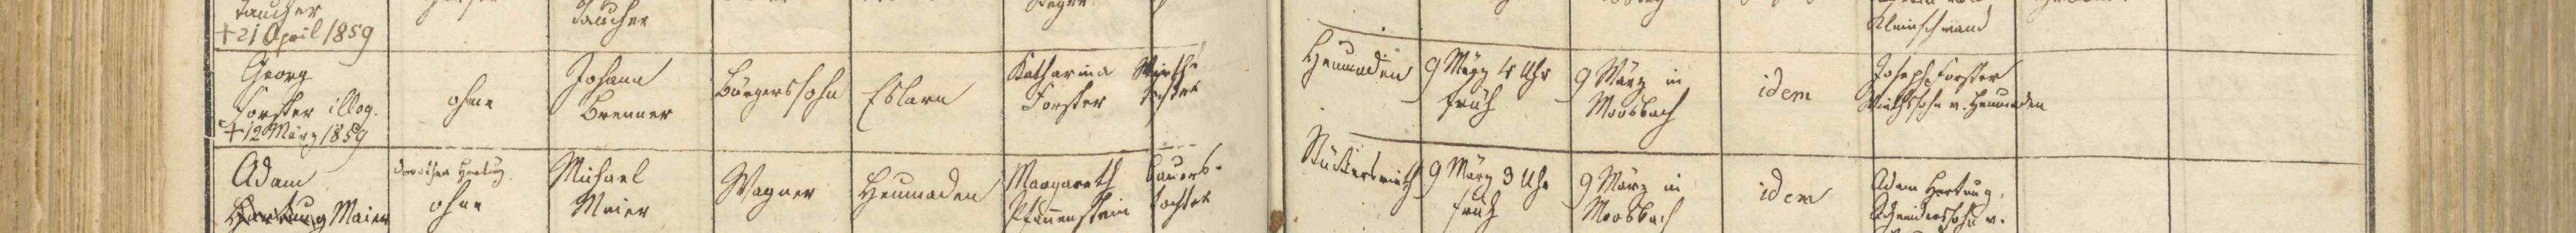
\includegraphics[width=0.85\linewidth,height=\textheight,keepaspectratio,alt={Livro de batismos de Moosbach, página 96: o batismo de Adam Meier, nascido em 9 de março de 1859, às três da madrugada, filho do fabricante de rodas Michael Meier e de Margaretha Pfannenstein, tendo por padrinho Adam Hartung, filho do ferreiro de Heumaden.}]{imagens/doc3_adam_meier_1859.jpg}
\caption{Livro de batismos de Moosbach, página 96: o batismo de Adam
Meier, nascido em 9 de março de 1859, às três da madrugada, filho do
fabricante de rodas Michael Meier e de Margaretha Pfannenstein, tendo
por padrinho Adam Hartung, filho do ferreiro de Heumaden.}
\end{figure}

O segundo batismo está na página 115, dois anos e meio depois, num
sábado de verão. Nome: \emph{Franziska Voit}. Pai: \emph{Johann Voit},
lavrador, de Treswitz, que é como o padre abreviou Burgtreswitz. Mãe:
\emph{Barbara Woppmann}. Nascimento: \emph{29. Juni, Morgens} (29 de
junho de 1861, pela manhã). Sem hora exata, desta vez. Batismo: no mesmo
dia, em Moosbach. E 29 de junho, observem, é o dia de São Pedro e São
Paulo: a menina nasceu e foi batizada exatamente na festa dos padroeiros
da paróquia. Imagino a igreja enfeitada, a missa solene, e no meio da
festa uma família de Burgtreswitz chegando com um bebê de poucas horas.

A parteira, segundo a transcrição, chamava-se Schmirl. A madrinha:
\emph{Margaretha Albrecht}, lavradora.

Albrecht. Li duas vezes. Durante anos achei que Albrecht era o sobrenome
da mãe de Josef Haas, a Maria Anna Albrecht de Stoffen, e sorri da
coincidência. Depois descobri que a Maria Anna de Stoffen nunca foi
nossa: era mãe de outro Joseph Haas. A piscadela da genealogia era maior
do que eu pensava. Os nomes se repetem, e é preciso ter cuidado com
eles.

\begin{ficha}

\textbf{Ficha do Arquivo}: Paróquia de St.~Peter und Paul, Moosbach.
Livro de batismos 1847--1904 (\texttt{Moosbach\_Leuchtenberg005}),
p.~115. Batizada: Franziska Voit. Pai: Johann Voit, \emph{Bauer} em
(Burg)Treswitz. Mãe: Barbara Woppmann (\emph{Woppman}). Nascimento: 29
de junho de 1861, pela manhã (\emph{Morgens}). Batismo: 29 de junho de
1861, em Moosbach. Parteira: Schmirl (segundo a transcrição do dossiê).
Madrinha: Margaretha Albrecht, \emph{Bäuerin}. Imagem:
\texttt{imagens/doc4\_franziska\_voit\_1861.jpg}.

\end{ficha}

\begin{figure}
\centering
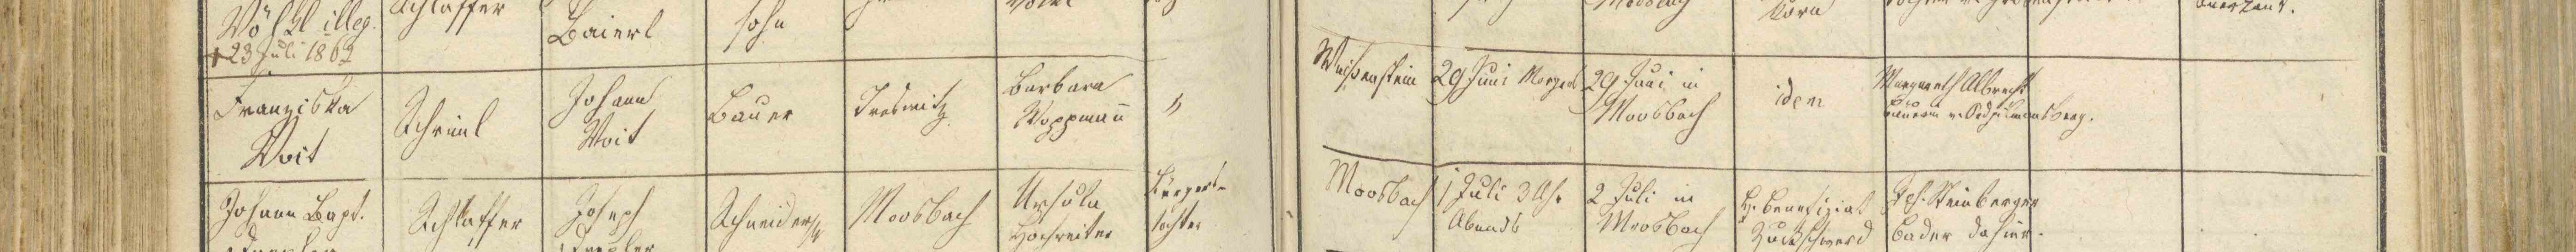
\includegraphics[width=0.85\linewidth,height=\textheight,keepaspectratio,alt={Livro de batismos de Moosbach, página 115: o batismo de Franziska Voit, nascida em 29 de junho de 1861, dia de São Pedro e São Paulo, filha do lavrador Johann Voit, de Burgtreswitz, e de Barbara Woppmann.}]{imagens/doc4_franziska_voit_1861.jpg}
\caption{Livro de batismos de Moosbach, página 115: o batismo de
Franziska Voit, nascida em 29 de junho de 1861, dia de São Pedro e São
Paulo, filha do lavrador Johann Voit, de Burgtreswitz, e de Barbara
Woppmann.}
\end{figure}

\section{O quebra-cabeça bávaro}\label{o-quebra-cabeuxe7a-buxe1varo}

Quando terminei de ler as quatro páginas, a metade bávara da árvore de
vocês estava completa até os tataravós do Fata e da Mota. Vou desenhá-la
em palavras, porque é assim que vocês vão se lembrar dela.

Em Heumaden, um fabricante de rodas chamado Michael Meier. Em
Rückersrieth, uma filha de lavrador chamada Margaretha Pfannenstein.
Deles nasce, numa madrugada de março de 1859, Georg Adam, que recebe o
nome do filho do ferreiro.

Em Burgtreswitz, um lavrador chamado Johann Voit e sua mulher, Barbara
Woppmann. Deles nasce, na manhã da festa dos padroeiros de 1861,
Franziska.

Adam e Franziska casam-se em Moosbach num domingo de novembro de 1884,
com os dois pais por testemunhas. Ele faz rodas; depois vive da terra.
Têm filhos: Maria Katharina em 1886, e depois, numa madrugada de abril
de 1888, Maria, a Mota. Mais tarde virão Theresia e Michael. Depois de
1892, a família some dos livros de Moosbach e reaparece, oitenta anos
depois, em cartas vindas da Saxônia.

A cinquenta quilômetros dali, em Leonberg, o operário Josef Haas, filho
de Michael Haas e Kunigunde Stadelmann, e Franziska Dengler têm um filho
chamado Johann.

Essas duas linhas vão se encontrar em algum momento antes de 1907. Não
sei onde, nem como. O casamento foi em Eibenstock, longe das duas
aldeias. Talvez ele tenha ido trabalhar como estucador em alguma obra
perto de Heumaden. Talvez ela tenha ido trabalhar em outro lugar, como
tantas moças do campo. Talvez tenham se conhecido numa festa, numa
feira, numa estação de trem. Não há documento. E é aqui que o meu
trabalho de pesquisador termina e começa o de vocês, se quiserem: o
livro de casamentos de Eibenstock existe, em algum arquivo da Saxônia, e
um dia alguém vai abri-lo.

Penso, ao terminar este capítulo, em tudo o que a Mota não contou. Ela
viveu oitenta e cinco anos, sessenta deles no Brasil, e os netos lembram
dela como uma avó de olhos azuis e poucas palavras em português, que
abraçava muito. Os nomes de Heumaden, de Burgtreswitz, do pai
\emph{Wagner}, do avô ferreiro do padrinho: nada disso chegou até nós
pela voz dela, ou chegou em pedaços: a palavra \emph{Heumaden} repetida,
um sotaque, uma lembrança de vacas. O resto ficou guardado na letra que
ela sabia ler e nós não. Foi preciso um neto aprender a
\emph{Kurrentschrift} para que ela, finalmente, nos contasse de onde
vinha.

Faltava um último ponto no mapa. Dez dias depois de Maxhütte-Haidhof, eu
estaria em pé sobre uma linha de metal, em Londres, no lugar onde a
humanidade combinou que começam todas as longitudes.

\section{Para vocês descobrirem}\label{para-vocuxeas-descobrirem-17}

\begin{itemize}
\tightlist
\item
  Katharina Reichenberger, a madrinha de Burgtreswitz, era a tia
  Katharina da tradição, nascida Meier e casada com um Reichenberger?
  Procurem o registro de casamento em Burgtreswitz, que eu ainda não li.
\item
  O que estava escrito antes do retoque no sobrenome de Adam, na página
  96? A imagem está em \texttt{imagens/doc3\_adam\_meier\_1859.jpg}. Foi
  mesmo uma legitimação?
\item
  Onde um estucador de Leonberg e uma moça de Heumaden se conheceram, e
  por que foram casar em Eibenstock? O livro de casamentos de lá está em
  algum arquivo da Saxônia, à espera de quem o abra.
\item
  Além da palavra \emph{Heumaden} e da lembrança das vacas, o que a Mota
  contou aos netos sobre a terra dela? Perguntem aos primos que a
  conheceram.
\end{itemize}

\chapter{Com os Pés no Meridiano Zero}\label{cap-19}

\emph{51,48° N · 0,00°, Observatório Real, Greenwich, Londres}

\begin{quote}
\emph{Toda medida começa num lugar escolhido. O que importa é medir a
partir dele com honestidade.}
\end{quote}

A linha que os turistas fotografam em Greenwich não é a longitude zero
que o celular deles usa.

\section{Uma linha de latão}\label{uma-linha-de-latuxe3o}

No dia 16 de fevereiro de 2018, uma sexta-feira, dez dias depois de
Maxhütte-Haidhof, eu estava em Greenwich, no alto da colina do
Observatório Real, sobre o rio Tâmisa, a leste do centro de Londres. Ali
há uma linha. É uma faixa de metal cravada no chão do pátio, que
atravessa as pedras e marca o meridiano de Greenwich, a longitude zero.
De um lado, o hemisfério oriental; do outro, o ocidental. Os turistas
fazem fila para pôr um pé de cada lado e tirar uma fotografia. Um
professor de Física que passou a vida ensinando coordenadas não está
imune a essa tentação; não há dignidade acadêmica que resista a uma
linha dessas, e o título deste capítulo não esconde de que lado da fila
eu estava.

Há uma história por trás da linha que eu conhecia antes de ir e que,
depois daquele inverno, ganhou para mim outro sentido. Até o século XIX,
cada país contava as longitudes a partir do seu próprio meridiano: os
franceses a partir de Paris, os espanhóis a partir de Cádiz, os
portugueses a partir de Lisboa ou de outros pontos, e assim por diante.
Mapas de nações diferentes não se encaixavam. Navios trocavam posições
que não batiam. Foi preciso uma conferência internacional, em
Washington, para que vinte e tantos países concordassem em adotar um
único meridiano de origem para o mundo inteiro. Escolheram Greenwich. A
conferência se reuniu em outubro de 1884.

Outubro de 1884. Três meses depois de Josef Haas assinar o assento nº 47
em Leonberg. Um mês antes de Adam Meier e Franziska Voit se casarem em
Moosbach. No mesmo outono em que as duas linhas bávaras de vocês estavam
sendo traçadas, a humanidade combinava de onde se contaria, dali em
diante, a posição de todas as coisas. Não há nenhuma relação de causa
entre os fatos, é claro. Mas um meteorologista vive de coincidências
temporais: é olhando o que acontece ao mesmo tempo em lugares diferentes
que se descobre a estrutura de um sistema. E eu gosto de pensar que o
Fata nasceu no ano em que o mundo ganhou um meridiano zero.

Volto ao celular, o detalhe técnico que faz a alegria dos físicos que
visitam Greenwich. A linha de metal marca o meridiano histórico,
definido pelo eixo de um telescópio instalado ali no século XIX. Mas o
sistema de referência usado hoje pelos satélites de posicionamento, o
que faz funcionar o GPS dos nossos celulares, coloca a longitude zero
uns cem metros a leste da linha de metal. A diferença vem do jeito como
cada sistema define a vertical e o formato da Terra. Quem fica com um pé
de cada lado da faixa e olha o celular descobre que, para o satélite,
está inteiramente no hemisfério ocidental.

Achei isso uma lição sobre genealogia. A origem que a família fotografa
e a origem que os documentos registram raramente coincidem com
perfeição. O Fata fazia aniversário em 8 de julho, segundo a planilha; o
registro civil diz 11. A Mota tinha 25 anos no manifesto e 24 na
realidade. A madrinha dela era a tia Katharina Meier na memória e
Katharina Reichenberger no livro. As duas origens existem, e a distância
entre elas é de uns poucos metros, uns poucos dias, um sobrenome de
casada. O trabalho do pesquisador é medir essa distância e dizê-la.

\section{Toda família escolhe seu
meridiano}\label{toda-famuxedlia-escolhe-seu-meridiano}

A longitude zero não é natural. É isso que eu sempre digo aos alunos e
que eles demoram a aceitar. A latitude tem uma origem física: o equador
é o círculo onde o eixo de rotação da Terra é perpendicular à
superfície, e qualquer civilização, em qualquer planeta, chegaria a ele.
Mas não existe nenhuma razão física para que a longitude zero passe por
Greenwich e não por Paris, por Roma ou por Florianópolis. É uma
convenção. Ainda assim, sem essa escolha nenhum mapa funciona.
Precisamos de um ponto a partir do qual contar.

Toda família faz o mesmo. Escolhe um ponto e conta a partir dele. Para
os mais de seiscentos descendentes que se reuniram em março de 2013, o
meridiano zero era a chegada de Johann e Maria ao Brasil, em 1913: o
centenário era contado a partir dali. Para a planilha do Agenor, o
meridiano zero era o casal, e tudo se contava em filhos, netos,
bisnetos, trinetos. Para este livro, o meridiano zero são vocês dois. A
árvore que montei diz isso com todas as letras: Matheus e Lucas são a
geração G1, e tudo o mais se conta para trás a partir de vocês: G2 para
os pais, G3 para os avós, até G8, os hexavós de Harderode e de
Schleswig-Holstein.

Escolhi assim porque é o único jeito de fazer caber, numa só árvore,
gente que nunca se encontrou. Os Haas da Baviera e os Lohmann da Baixa
Saxônia nunca souberam uns dos outros. Os Michels de Hermeskeil e os
Funke de Joinville viveram em séculos diferentes. O ponto onde todas
essas linhas se cruzam é uma casa em Florianópolis onde moram dois
meninos (hoje, dois homens). Vocês são a interseção. Por isso são a
origem.

Quero dizer uma coisa sobre isso, já que estou de pé sobre uma origem
arbitrária. Ser o meridiano zero de uma família é uma responsabilidade.
É a partir de vocês que alguém, um dia, vai contar as gerações de novo.
Daqui a cem anos, os filhos dos filhos de vocês vão escolher o próprio
meridiano, e vocês serão G2, G3, G4. Vão estar no meio da árvore, não na
ponta. Isso é o que acontece com todo mundo. Aconteceu com o Fata e a
Mota, que um dia foram o centro de tudo e hoje são G4.

Há uma imagem da minha profissão que resume isso melhor do que eu
consigo. Chama-se circulação geral da atmosfera. Se vocês olharem o
planeta inteiro de longe, o vento parece caótico: tempestades aqui,
calmarias ali, frentes, ciclones, brisas. Mas, na média de muitos anos,
ele se organiza em grandes células que dão a volta ao mundo. Perto do
equador, o ar quente sobe, corre em altitude para os polos, desce por
volta dos trinta graus de latitude e volta junto ao chão como os
alísios: é a célula de Hadley, que empurrou os veleiros de 1828 e de
1847 e os prendeu nas calmarias. Mais para o alto das latitudes, outras
células, outros ventos: os de oeste que varrem a Europa e o sul do
Brasil, o ar polar que desce em ondas. Nenhuma dessas células existe
sozinha. Cada uma depende das vizinhas. O ar que sobe em Belém um dia
desce no Saara ou no Atlântico Sul; o frio que nasce na Antártida um dia
chega a Vidal Ramos como geada. É um único sistema.

Uma família é assim. Vista de perto, é uma confusão de gente que nasce,
casa, briga, emigra, morre, perde contato, muda de nome e de língua.
Vista de longe, ao longo de duzentos anos, é uma circulação. Gente que
sobe do Mosela e desce em Desterro. Gente que sai do Alto Palatinado e
chega ao Rio de Janeiro. Gente que vai do litoral para o Alto Vale, do
Alto Vale para o Paraná, do Rio Grande para Joinville, de Joinville e de
Vidal Ramos para Florianópolis. De vez em quando, alguém faz o caminho
de volta, como eu fiz naquele inverno, fechando a célula.

\section{As coordenadas da família}\label{as-coordenadas-da-famuxedlia}

A árvore que exportei do FamilySearch tem cinquenta e oito coordenadas
geográficas. São os lugares onde a família nasceu, casou, morreu,
chegou. Penso nelas como se as recitasse de pé sobre a longitude zero,
aproximadas, como quem reza um terço. Faço isso aqui para vocês,
devagar, de leste para oeste, porque é a direção em que a família andou.

O ponto mais oriental de todos é a Baviera. Leonberg, hoje
Maxhütte-Haidhof, a 49,2 norte e 12,1 leste. Heumaden, Rückersrieth e
Burgtreswitz, em volta de Moosbach, a 49,6 norte e 12,4 leste. Esses são
os Haas, os Meier, os Voit.

Um pouco a oeste e ao norte, a Baixa Saxônia: Harderode, a terra dos
Lohmann, perto de Hameln, a 52 norte e 9,4 leste, e mais ao norte ainda
Schleswig-Holstein, de onde vieram os Schnack. São a família da mãe de
vocês.

Depois, descendo para o sudoeste, a Renânia e o Mosela, a terra dos que
vieram primeiro. Solingen, a cidade das lâminas, de onde a tradição faz
vir os Doerner e os Lauterjung, a 51,2 norte e 7,1 leste, quase
exatamente a latitude de Greenwich, onde eu estava. Pünderich, na curva
do Mosela, a terra de Angela Catharina Arns, a 50 norte e 7,1 leste.
Hermeskeil, onde nasceu o menino Anton Michels, e Schweich, de Bernard
Preis, os dois perto de Trier, a uns 49,7 norte e menos de 7 graus
leste.

Então, a linha zero. Greenwich. O único lugar desta lista que não tem
nada a ver com a família, a não ser o fato de eu ter estado ali.

Depois, o oceano. Do outro lado, invertendo o sinal da latitude e da
longitude, como quem atravessa um espelho: o Rio de Janeiro, onde o
\emph{Formosa} deixou a família em 26 de março de 1913, a 22,9 sul e
43,2 oeste; e Laguna, a porta de Santa Catarina que a tradição aponta, a
28,5 sul e 48,8 oeste. São Pedro de Alcântara, a primeira colônia alemã
de Santa Catarina, a 27,6 sul e 48,8 oeste. Anitápolis e o Rio do Ouro,
o Lote 17, a 27,9 sul e 49,1 oeste. São Martinho e Vargem do Cedro, a
terra dos Preiss e dos Michels, a pouco mais de 28 sul. Brusque, onde
estão Fernando Dörner e Gertrudes Preiss, a 27,1 sul. Ituporanga, Rio
Novo, Águas Negras, a 27,4 sul e 49,6 oeste. Vidal Ramos, a casa dos
meus pais, a 27,4 sul e 49,4 oeste. Aurora e Ribeirão das Pacas, onde
estão o Fata e a Mota cercados dos túmulos que ele fez, a 27,3 sul e
49,6 oeste. Mais ao sul e a oeste, no Rio Grande, Estrela e Arroio do
Meio, a casa dos Lohmann em Palmas, à beira do Taquari, a 29,3 sul e
51,9 oeste. Joinville, a terra dos Funke e da Oma Rosita, a 26,3 sul e
48,8 oeste. E, finalmente, Florianópolis, a 27,6 sul e 48,5 oeste. A
casa de vocês.

Notem uma coisa que só um meteorologista acharia digna de nota: as duas
metades da família vivem em estações trocadas. Quando é inverno em
Heumaden, é verão em Aurora. A Mota nasceu numa primavera bávara, em
abril, e chegou ao Brasil no fim de um verão, em março, e no primeiro
ano em Santa Catarina deve ter estranhado o Natal com calor e o dia de
São João, que na Baviera é festa de verão, com frio. Para os bisnetos
dela, que são vocês, julho é mês de casaco e dezembro é mês de praia; em
Heumaden, cada aniversário de vocês cairia na estação oposta. O Fata,
que nasceu em julho, num verão bávaro, passou mais de cinquenta
aniversários no Brasil, todos eles no inverno. Nunca saberei se sentia
falta do verão no dia do aniversário. Imagino que sim.

Se vocês desenharem todos esses pontos num mapa, vão ver duas nuvens:
uma no centro da Europa, entre 48 e 54 graus norte, e outra no sul do
Brasil, entre 26 e 30 graus sul. Entre as duas, o Atlântico inteiro,
cortado por setas: 1828, 1846, 1847, 1913. Todas as setas, de um modo ou
de outro, terminam no mesmo ponto. Uma sugestão que deixo à editora, se
este livro tiver uma: esse mapa deveria ser a guarda do volume, a
primeira coisa que se vê ao abri-lo.

\section{Três rios, uma só chuva}\label{truxeas-rios-uma-suxf3-chuva}

Há uma coisa que a nuvem brasileira de pontos mostra e que a europeia
não mostra: quase todos estão à beira de um rio. Contei isso na Parte V,
e só retomo aqui o essencial, porque em Greenwich, diante do Tâmisa,
pensei nos nossos rios.

O Tubarão, que desce da serra e deságua na laguna, e que em março de
1974 matou cerca de duzentas pessoas, nos números mais citados, e afogou
a cidade, sessenta e um anos depois do ano em que, segundo a tradição,
os Haas passaram por Laguna, na boca desse mesmo rio. O Itajaí, com seus
braços, o do Sul passando por Ituporanga, onde a Barragem Sul foi
construída depois das grandes cheias, e o Itajaí-Mirim passando por
Brusque, onde estão os pais da vó Adelina; o rio das enchentes de 1880,
de 1911, de 1983, de 1984, de 2008, de 2011. E o Taquari, no Rio Grande,
diante do qual fica a casa dos Lohmann, e que em maio de 1941, em
setembro e novembro de 2023 e em maio de 2024 subiu além de tudo o que a
família tinha visto.

Os imigrantes se instalaram à beira dos rios porque a água era estrada,
era força para o moinho, era terra plana e fértil nas várzeas. E porque
não sabiam. Ninguém lhes contou que aqueles rios podiam subir mais de
dez metros em poucos dias. Os três rios da família são alimentados pela
mesma máquina atmosférica: a umidade que vem da Amazônia, carregada para
o sul por uma corrente de vento que corre baixa, a leste dos Andes; as
frentes que estacionam sobre o Sul do Brasil; os ciclones que se formam
na costa; e, nos anos de El Niño, a chuva que não para. Três rios, uma
só chuva. É o meu trabalho estudar essa chuva. Não escolhi esse trabalho
por causa da família. Mas, depois de escrever este livro, não consigo
mais separar uma coisa da outra.

Houve também a herança, que foi o assunto do capítulo 15. Na Europa, a
terra que se dividia até não sobrar nada, no Mosela e no Hunsrück,
empurrando os Michels, os Arns e os Preis para o mar; e a terra que
passava inteira a um só filho, na Baviera antiga, empurrando os outros
para as oficinas e as usinas, como o operário Josef. No Brasil, o lote
colonial e as famílias de dez, doze, quinze filhos (o Fata teve onze, o
trisavô Carlos Doerner teve quinze, Francisco Lohmann teve doze) e,
outra vez, a necessidade de partir: para o Alto Vale, para o Oeste, para
o Paraná. Em quase todos os ramos há gente que não ficou com a terra e
por isso andou. Vocês são o resultado de muitos que não herdaram.

\section{Os Andes, brevemente}\label{os-andes-brevemente}

Quero falar dos Andes porque eles fecham um círculo, mas vou ser breve,
como prometi a mim mesmo quando planejei este livro.

Em outra viagem, com a mãe de vocês e com vocês dois, atravessamos a
cordilheira e estivemos em Valparaíso, em Santiago, em Valle Nevado. Não
vou contar essa viagem aqui. Ela é de vocês, e vocês a contarão do jeito
que quiserem, se quiserem. Quero só registrar o que ela significou na
geometria deste livro.

Os Andes são, para o clima do Sul do Brasil, o que os Alpes são para a
Europa: uma parede. É por causa deles que a umidade da Amazônia, em vez
de escapar para o Pacífico, é desviada para o sul e chega aos vales do
Itajaí e do Taquari como chuva. Sem os Andes, os três rios da família
seriam outros. Cada enchente que contei na Parte V tem parte da sua
origem numa encosta andina.

Foi ali, naquela parede, que vi vocês fazerem a própria travessia, a de
quem já não precisa ir embora para sobreviver e por isso pode ir para
conhecer. Johann e Maria cruzaram os Alpes para nunca mais voltar. Eu
cruzei os Alpes para buscar um papel e voltei. Vocês cruzaram os Andes e
voltaram também, e cruzarão outras montanhas, e não sei quais. A
bússola, a esta altura, já estava passando de mão.

\section{A volta}\label{a-volta}

De Greenwich, o que guardo com segurança são a data e a linha. O resto é
o que fevereiro em Londres costuma fazer com os pés de um catarinense, e
a cabeça cheia de números que um lugar desses deixa em qualquer físico.

Na pasta, eu levava a cópia do assento nº 47, de Leonberg. Levava as
referências dos quatro registros de Moosbach. Levava a informação de que
um Haas nascido em Leonberg em 1941 constava nos registros da cidade.
Levava, sobretudo, a sensação rara, que os meteorologistas conhecem
pouco, de que uma previsão tinha se confirmado. A pergunta que movia
este livro, \emph{ainda há alguém do outro lado?}, tinha uma resposta.
Sim. Há livros com os nomes deles, e há pelo menos uma pessoa com o
sobrenome deles, na mesma cidade.

Faltava levar isso para casa. Para a casa de Florianópolis, onde estão
vocês. E para a casa de Vidal Ramos, onde estava a última pessoa viva da
geração que tinha conhecido o Fata e a Mota de perto: a minha mãe, a vó
Adelina, a nora deles, que entrou na família em 1947 e conviveu com eles
por mais de duas décadas.

Ela estava com 91 anos naquele fevereiro. Viveria mais um.

A volta para casa, fosse qual fosse o caminho, cruzaria de novo, sem
cerimônia, todas as linhas que eu tinha passado a vida ensinando a
desenhar. O equador, onde o sinal da latitude se inverte. O trópico. A
longitude zero ficaria para trás, depois a de 10 graus oeste, a de 20, a
de 30, a de 40. Quando chegássemos a 48,5, estaríamos em casa.

\section{Para vocês descobrirem}\label{para-vocuxeas-descobrirem-18}

\begin{itemize}
\tightlist
\item
  O Haas nascido em Leonberg em 1941, de quem eu levava notícia na
  pasta, é parente de vocês? Só um documento decide.
\item
  De onde veio o 8 de julho que o Agenor anotou na planilha, se o
  registro civil diz 11? Perguntem aos primos em que dia a família
  festejava o aniversário do Fata.
\item
  Quantas das cinquenta e oito coordenadas da árvore ficam longe de um
  rio? Desenhem o mapa e contem.
\item
  Quem mais, entre os descendentes do Fata e da Mota, fez o caminho de
  volta à Europa? Perguntem aos vivos.
\end{itemize}

\chapter*{Epílogo --- A Bússola Entregue a Matheus e
Lucas}\label{epilogo}
\addcontentsline{toc}{chapter}{Epílogo --- A Bússola Entregue a Matheus
e Lucas}

\emph{27,4° S · 49,4° O, Vidal Ramos · 27,6° S · 48,5° O, Florianópolis}

\begin{quote}
\emph{A árvore nunca termina. Ela apenas muda de mãos.}
\end{quote}

\section{Vinte e dois de fevereiro de
2019}\label{vinte-e-dois-de-fevereiro-de-2019}

A vó Adelina morreu em Vidal Ramos no dia 22 de fevereiro de 2019. Tinha
92 anos. Fazia pouco mais de um ano que eu estivera diante do livro de
1884 em Maxhütte-Haidhof, e pouco mais de cinco que o vô Baldoíno se
fora, em dezembro de 2013.

Não vou escrever muito sobre esse dia. Há coisas que um filho guarda
para si, e este livro, desde o começo, fez a promessa de contar só o que
pode mostrar. A morte de uma mãe não se mostra. Diz-se a data, e quem
leu até aqui sabe o resto.

Quero dizer quem ela foi para esta história, porque sem ela não haveria
livro. Adelina Doerner nasceu em 30 de outubro de 1926, em São Martinho,
filha de Fernando Dörner e de Gertrudes Preiss. Pelo pai, descendia dos
Dörner da Renânia, que a tradição liga aos cuteleiros de Solingen, e dos
Eller da Vestfália. Pela mãe, dos Preis de Schweich, dos Michels de
Hermeskeil, da longeva Angela Catharina Arns de Pünderich. Casou com
Baldoíno Haas em 1947 e juntou, sem saber que fazia isso, as duas
grandes correntes deste livro: a de 1828 e 1847, que chegou de veleiro e
abriu as primeiras clareiras perto de Desterro, e a de 1913, que chegou
de vapor e subiu para o Alto Vale. Em maio de 2012, nas Bodas de 65
anos, deixou-se gravar diante de uma câmera, dizendo nomes de tios, de
lugares, de rios. Esse vídeo foi o primeiro documento desta pesquisa. A
voz dela abre o livro, no capítulo 1, e é justo que a sua ausência o
feche.

Ela conheceu o Fata e a Mota. Era nora deles e conviveu com os dois por
mais de duas décadas. Quando o Fata morreu, em 1969, eu ainda não tinha
quatro anos. Quando a Mota morreu, em 1973, eu tinha oito. As minhas
lembranças deles são esgarçadas, quase sombras. As dela eram inteiras.
Durante anos, ela foi a última testemunha viva, na nossa casa, de como
eles falavam, andavam, riam.

Gostaria de poder escrever aqui que, ao voltar da Baviera, sentei ao
lado dela na cozinha de Vidal Ramos e pus nas mãos dela a cópia do
assento nº 47, a assinatura de Josef Haas, a página 441 de Moosbach com
o nome da sogra dela, e que ela olhou aquilo tudo e disse alguma coisa
que eu pudesse transcrever. Seria a cena perfeita para fechar o livro.
Mas não vou escrevê-la como fato, porque este livro não tem o direito de
inventar a vó Adelina. Fica a pergunta, que me faço desde então: o que
ela teria dito? Teria reconhecido na letra gótica a letra das cartas que
a Mota talvez recebesse da Alemanha? Teria achado graça da data do Fata,
11 e não 8 de julho? Teria dito que já sabia, que sempre soube, que
Heumaden existia? Não sei. Deixo a pergunta escrita, que é o que se faz
com as perguntas que não têm mais a quem ser feitas.

Com ela fechou-se uma geração. Do lado do pai de vocês, já não resta
ninguém que tenha ouvido a voz do Fata e da Mota como adulto. Restam os
netos, meus primos, que eram crianças nos anos de Ribeirão das Pacas e
que ainda guardam fragmentos. Restam também o texto de Marise, a
planilha do Agenor e os papéis. E restam vocês.

\section{O novo lote}\label{o-novo-lote-1}

Quando Johann e Maria chegaram a Rio do Ouro, em 1913, a primeira coisa
que fizeram foi comprar um pedaço de terra. O Lote 17. Uma colônia, como
se dizia, uns vinte e cinco hectares de mato, comprados junto com um
amigo. A terra era ruim, seca e ácida, e eles acabaram indo embora cinco
anos depois. Mas o lote foi o começo. Foi nele que nasceram Fernando e
Alexandre, foi nele que o Fata aprendeu a fazer túmulos de granilite com
anjos de gesso para comprar o pão. Foi o primeiro chão dos Haas no
Brasil.

Cada geração de imigrantes recebia ou comprava um lote, trabalhava nele,
e depois o passava adiante, a um filho que ficava, enquanto os outros
partiam para abrir lotes novos mais longe. Essa foi a forma de herança
das colônias do Sul, e foi ela que espalhou os descendentes do Fata por
Ituporanga, Vidal Ramos, Aurora, pelo Paraná.

Eu não tenho um lote para deixar a vocês. Tenho outra coisa, e passei os
últimos anos cuidando dela como o Fata cuidava da roça de Rio Novo.

Chama-se, sem nenhuma poesia, um repositório. Um conjunto de pastas e
arquivos guardados num servidor, com controle de versões, de modo que
cada mudança fica registrada com data e autor, e nada se perde. Ali
estão as imagens dos documentos: o casamento de Josef Haas em Leonberg,
o assento nº 47 de Leonberg, o manifesto do \emph{Formosa}, os quatro
registros de Moosbach, o casamento de Carlos Doerner com Hulda Peters em
Capivari, as certidões de óbito de Fernando Dörner e Gertrudes Preiss em
Brusque. Estão as fotografias: o Fata e a Mota com os sete filhos, as
Bodas de Ouro, a despedida de março de 1913, os tios-avós Lohmann em
Arroio do Meio, o Vô Erno com os alunos, a Oma Dora com os irmãos, as
quatro gerações na garagem de Joinville. Estão as cartas de Rempesgrün.
Está a árvore exportada do FamilySearch, com as cinquenta e oito
coordenadas. Está a planilha do Agenor, convertida e preservada. Estão
os pequenos programas em Python que escrevi para organizar tudo isso,
porque um cientista não consegue deixar de transformar a família num
banco de dados, e porque descobri, no caminho, que os dados insistem em
virar gente. Está o texto do centenário. Está o roteiro deste livro e,
agora, o próprio livro.

É uma cápsula do tempo, mas viva, porque pode ser aberta, corrigida,
aumentada. Quando alguém encontrar o registro de óbito de Luisa e Walter
em Anitápolis, ou o registro do traslado para Ituporanga, ele entra ali.
Quando alguém abrir o livro de casamentos de Eibenstock, ele entra ali.
Quando alguém descobrir quem era Katharina Reichenberger, a madrinha de
Burgtreswitz, ele entra ali. O repositório é o novo lote: um chão que se
recebe, se trabalha e se passa adiante.

Ele tem uma diferença para os lotes antigos: não se divide. Na Europa
dos nossos antepassados, a terra que se repartia entre os filhos ia
ficando cada vez menor, até não sustentar ninguém, e as famílias
precisavam emigrar. Na Baviera, a terra que passava inteira a um só
filho deixava os outros sem nada, e eles iam para as olarias e as
usinas. Este lote, não. Cada um de vocês pode ter uma cópia inteira.
Cada primo, cada um dos mais de seiscentos descendentes de Johann e
Maria, pode ter uma cópia inteira. É a primeira herança da família que
não precisa ser partilhada nem negada a ninguém.

Como todo lote, ele precisa de quem o trabalhe. Um repositório
abandonado é como uma colônia abandonada: o mato toma conta. Os formatos
de arquivo envelhecem, os servidores mudam, os links quebram. Daqui a
trinta anos, alguém vai precisar abrir aquelas pastas e convertê-las
para o que existir então. Esse alguém, espero, será um de vocês. Ou um
filho de vocês.

\section{Carta a Matheus e Lucas}\label{carta-a-matheus-e-lucas}

Matheus, Lucas.

Escrevi este livro para vocês, e chegou a hora de dizer o que eu queria
dizer desde o prólogo.

Quando vocês eram pequenos, eu ficava às vezes olhando os dois à mesa e
me perguntando de quantas aldeias, portos, ofícios e milagres de
sobrevivência eram feitos dois meninos catarinenses do século XXI. Agora
eu sei um pouco mais. Não sei tudo. Ninguém sabe tudo de onde veio, e
quem diz que sabe está inventando. Mas sei o bastante para dizer a vocês
o que vocês carregam.

Vocês carregam nas mãos o prumo de pedreiro e a arte em gesso de Johann
Haas, o Fata, que fez igrejas em Ituporanga e anjos para os túmulos de
gente pobre, e que hoje dorme em Aurora entre os anjos que ele mesmo
moldou. Carregam a doçura silenciosa de Maria Meier, a Mota, que nunca
aprendeu o português e, mesmo assim, se fez entender pelos netos com um
abraço demorado e um olhar azul. Carregam as rodas de madeira de
Heumaden, que o tataravô Michael Meier e o filho dele, Adam, faziam para
as carroças do Alto Palatinado, e o aro de ferro que o ferreiro de
Heumaden forjava em volta delas. Carregam o turno de fábrica do operário
Josef Haas, em Leonberg, que assinou com a mão trêmula o registro do
filho que ia atravessar o mundo.

Carregam o aço das forjas de Solingen dos Doerner e dos Lauterjung.
Carregam a coragem de um menino de seis anos chamado Anton Michels,
desembarcando em Desterro em 1828 numa terra que não esperava por ele.
Carregam a longevidade de quase um século de Angela Catharina Arns, que
nasceu numa curva do Mosela e morreu em Vargem do Cedro poucos meses
depois de nascer o vô Baldoíno. Carregam a fé dividida e reconciliada de
uma família de católicos e luteranos que, em 1900, precisou de uma
dispensa para casar e que hoje mal se lembra de que um dia isso foi um
problema.

E carregam, do lado da mãe de vocês, a outra metade, que eu conheci por
casamento e aprendi a amar como minha: a luz, a música e o afeto dos
Funke e dos Hoeveler; a medicina do avô Carlos Heinz, que deu nome a uma
escola e a um posto de saúde em Pirabeiraba; as salas de aula do Vô Erno
em Estrela e Nova Petrópolis; a persistência dos Lohmann, dos Schnack e
dos Endres no Vale do Taquari, numa casa diante de um rio que voltou a
subir em 2024; o segundo nome de Miguelina, \emph{Leocádia}, que passou
à avó Ilusca como quem passa um anel.

Carregam também as perdas. Hildegard e Frida, que morreram na Alemanha
antes de qualquer viagem. Luisa e Walter, que embarcaram em Marselha com
dois anos e com um, chegaram vivos ao Rio e morreram pequenos em Rio do
Ouro. O pequeno João, de 1932. Suzana Regina Schnack, que morreu vinte e
seis dias depois de dar à luz o trisavô Francisco. Quando eu estava em
Laguna em 2012, com vocês ao meu lado, pensei que vocês tinham mais ou
menos a idade de quem não cresceu. Penso nisso de novo cada vez que olho
a linha número 36 de Moosbach. Cada um de nós está vivo porque, em algum
momento, alguém sobreviveu a um inverno, a uma travessia, a uma febre.
Devemos isso a eles.

E carregam, por fim, os rios. O Tubarão, o Itajaí, o Taquari. Os nossos
antepassados assentaram as casas à beira da água porque a água era
estrada e força e terra boa, e não sabiam o que os rios eram capazes de
fazer. Nós sabemos. É uma das poucas vantagens que temos sobre eles:
medimos, modelamos, prevemos. Usem isso. Onde quer que vocês construam
as casas de vocês, olhem antes para o rio.

Agora, o que eu peço.

Peço que vocês terminem o que eu não terminei. Há um livro de casamentos
em Eibenstock, na Saxônia, que ninguém da família abriu. Há os livros da
Hospedaria da Ilha das Flores, no Arquivo Nacional, que dirão por onde a
família entrou em Santa Catarina. Há livros de óbitos em Anitápolis e o
registro do cemitério de Ituporanga, que guardam as datas de Luisa e
Walter. Há, em algum cartório ou paróquia, o nascimento da tia
Gertrudes. Há um registro de casamento em Burgtreswitz que talvez
explique quem era Katharina Reichenberger. Há o lugar e o ano
verdadeiros do nascimento de Ignazia Loch. Há tanta coisa. Uma árvore
genealógica nunca está pronta, do mesmo jeito que uma previsão do tempo
nunca é a última: sempre chega uma observação nova.

Peço uma coisa mais difícil. Em Maxhütte-Haidhof, em fevereiro de 2018,
eu soube que um Haas nascido em Leonberg em 1941 vivia ali. Não escrevi
o nome dele neste livro e não vou escrever. Ele tem direito à sua vida,
e a lei e o bom senso protegem esse direito. Mas a porta continua lá. Se
um dia vocês quiserem, com respeito, com cuidado, com a paciência que se
deve a um desconhecido que talvez seja da família, vocês podem escrever
uma carta. Talvez ele responda. Talvez já não esteja lá; os vizinhos
disseram que um Haas de mesmo nome morreu e que as filhas vivem na
Áustria. Talvez não seja parente nenhum. E há o endereço das cartas
guardadas pela família, em Falkenstein, no Vogtland, para onde também se
pode escrever. A pergunta que moveu este livro, \emph{ainda há alguém do
outro lado?}, merece ser feita em voz alta pelo menos uma vez. Eu a fiz
por escrito, neste livro. A voz pode ser de vocês.

Não estou pedindo que vocês sejam genealogistas. Sejam o que quiserem. O
texto do centenário termina com uma lista do que os descendentes de
Johann e Maria se tornaram (mães e pais de família, agricultores,
pedreiros, professores, cozinheiros, médicos, engenheiros, marceneiros,
advogados, cientistas, artistas) e conclui que, se o que nos define é o
que somos, então somos todos seres humanos tão comuns e tão especiais
quanto eles. Concordo com a Marise. Vocês não precisam carregar o
passado como um peso. Basta carregá-lo como uma bússola: uma coisa
pequena, que cabe no bolso, e que diz de onde se veio quando é preciso
decidir para onde ir.

Na minha profissão, quando queremos saber de onde veio uma massa de ar,
fazemos uma retrotrajetória: partimos do ponto onde ela está e
calculamos o caminho para trás, hora a hora, até a origem. Este livro
inteiro foi uma retrotrajetória. Parti de vocês, em Florianópolis, e
voltei, passo a passo, até uma siderúrgica em Sandberg, um prado de feno
em Heumaden, uma forja em Solingen, uma curva do Mosela. Agora que
cheguei ao fim, entrego o modelo a vocês para que o rodem no outro
sentido. Para a frente. Para onde eu não posso ir.

A penúltima imagem que deixo é esta. No cemitério de Aurora, no Alto
Vale do Itajaí, há túmulos com anjos de gesso feitos por um fabricante
de lápides nascido em Leonberg que chegou ao Brasil em 1913 com a
mulher, dois filhos pequenos e quase nada nas malas. Ele está enterrado
ali, ao lado dela, entre os anjos que moldou para os outros. Os anjos
não têm nome. Que eu saiba, ele não os assinou. Mas quem sabe olhar
reconhece a mão.

A última imagem é um mapa da Saxônia por volta de 1910. Glauchau e
Chemnitz ficam a poucas dezenas de quilômetros uma da outra. Em
Glauchau, segundo os registros do FamilySearch, nasce em 1910 Oscar
Martin Funke, o avô de Bárbara. Em Chemnitz, segundo a lembrança da
família, moram Johann e Maria Haas, que partem em 1913. Nenhum papel diz
que se cruzaram, e o mais provável é que nunca tenham sabido uns dos
outros.

Depois, cada linha faz o seu caminho. Os Haas passam por Marselha, pelo
Rio de Janeiro, por Rio do Ouro e por Ituporanga, e o caçula dos homens
que ficaram, meu pai, vai para Vidal Ramos. Os Funke chegam a Joinville,
onde nasce em 1939 o filho de Oscar, Carlos Heinz. Do lado dos Haas e do
lado dos Funke, ainda entram na conta o Mosela, Solingen, o Taquari, a
Suíça. E em 30 de setembro de 1995, às sete da noite, na igreja da
Comunidade Evangélica de Florianópolis, um neto de Johann casa com uma
neta de Oscar, oitenta e dois anos depois do \emph{Formosa}. As duas
linhas saíram de perto uma da outra e levaram quase um século para se
encontrar do outro lado do mar. Vocês nasceram desse encontro.

Vocês sabem olhar agora.

A bússola é de vocês.

Com todo o amor do pai de vocês,

Reinaldo

\emph{Florianópolis}

\chapter*{Nota sobre as Fontes e os Enigmas em
Aberto}\label{nota-fontes}
\addcontentsline{toc}{chapter}{Nota sobre as Fontes e os Enigmas em
Aberto}

Este livro foi escrito com documentos, memórias e dúvidas, nessa ordem
de confiança. Quando um documento e uma lembrança discordaram, fiquei
com o documento, e a lembrança passou a ser uma pergunta. Quando dois
documentos discordaram, deixei os dois à vista. As reconstituições (o
frio de uma madrugada em Heumaden, o porão de um navio, a cabana na mata
de Rio Novo) vêm sinalizadas no texto com palavras como \emph{imagino},
\emph{é provável}, \emph{conta-se}. O resto vem dos papéis.

\section{As fontes principais}\label{as-fontes-principais}

A pesquisa foi feita em três frentes. A primeira foram os registros do
FamilySearch, os índices e, sempre que possível, as imagens dos livros
paroquiais e civis do Brasil e da Alemanha. A segunda foram os livros de
batismo, casamento e óbito das paróquias católicas alemãs, lidos página
por página com a ajuda de um assistente de inteligência artificial, o
Antigravity, que percorria os livros digitalizados à procura dos nomes.
A terceira foi a árvore genealógica do meu primo Agenor Haas, montada ao
longo de anos. Onde as três discordam, o documento original vale mais
que o índice, e o índice vale mais que a árvore.

Para a família Haas, as fontes principais são os documentos da época: a
lista de passageiros do vapor \emph{Formosa}, os registros civis e
paroquiais e os registros de cemitério. Vêm depois a grande planilha
genealógica de Agenor Haas e, por fim, o texto \emph{História de João e
Maria Meyer Haas}, escrito por Marise Haas Lourenço para o centenário de
30 de março de 2013. Esse texto reuniu a memória da família e foi o
ponto de partida da pesquisa, mas, onde pode ser comparado com
documentos, erra com frequência. Afirma, por exemplo, que o desembarque
no Rio foi recusado, que houve muitas mortes a bordo e que Luisa e
Walter morreram nos barracões de Laguna. A lista de bordo e os
sepultamentos desmentem essas afirmações. Por isso, neste livro, ele
vale como tradição, não como fonte. Aos documentos se soma a fotografia
de despedida \emph{``Zum Andenken! vor unserer Abreise nach Brasilien,
7. März 1913''}; a lista de passageiros do \emph{Formosa} foi assinada
no Rio de Janeiro em 26 de março de 1913. Há também os testemunhos orais
que ouvi diretamente: o de meu pai, Baldoíno, sobre o traslado dos
restos dos irmãos de Anitápolis para Ituporanga, e o de meu avô Fernando
Dörner, sobre os anos de Vidal Ramos. Há ainda o assento nº 47 de 1884
do registro civil de Leonberg, hoje Maxhütte-Haidhof; o casamento de
Joseph Haas e Franziska Dengler em Leonberg, em 1878, que mostrou que o
batismo de Stoffen, de 1847, usado nas primeiras versões deste livro,
era de um homônimo; e quatro assentos dos livros paroquiais de St.~Peter
und Paul, em Moosbach (1859, 1861, 1884 e 1888).

Para os ramos Doerner, Preiss, Michels, Arns e Loch, usei os registros
reunidos no FamilySearch e os estudos de Toni Jochem e colaboradores
sobre as colônias de São Pedro de Alcântara, Santa Isabel e Piedade.
Também entram o Recenseamento de 1920, a imagem do assento do casamento
de Carlos Dörner com Hulda Peters, em 1900, e as certidões de óbito de
Fernando Dörner e Gertrudes Preiss, em Brusque.

Para os ramos de Bárbara (Lohmann, Schnack, Endres, Hoeveler e Funke),
usei o acervo fotográfico da família e os registros do FamilySearch.
Somam-se a eles os dossiês da CAPEF de Estrela sobre as famílias
fundadoras e a história da Fazenda Lohmann, em Roca Sales. Por fim, há
as reportagens e homenagens ao Dr.~Carlos Heinz Funke, em Joinville, e o
perfil topográfico e hidrológico da Casa Lohmann, em Palmas, Arroio do
Meio.

Quase todos esses materiais estão no repositório digital da árvore
genealógica, que acompanha este livro. As exceções são os que pertencem
a terceiros e a planilha de Agenor, que contém dados de parentes vivos e
fica no arquivo privado da família. No repositório está também a lista
completa das perguntas ainda abertas, com os arquivos onde procurar cada
resposta (\texttt{docs/questoes\_pesquisa\_antigravity.md}). As
respostas a essas perguntas, levantadas com ajuda de um assistente de
pesquisa, estão em \texttt{docs/respostas\_pesquisa\_antigravity.md}.
Usei delas só o que consegui conferir nos registros do FamilySearch ou
nas próprias imagens. Ao conferir, encontrei também leituras de
certidões com detalhes que a imagem não traz, como a hora e o médico do
óbito de Gertrudes Preiss, trocados com os do termo vizinho. Por isso,
aquele documento deve ser lido como um mapa de pistas, não como fonte.

\section{Enigmas que ficam para a próxima
geração}\label{enigmas-que-ficam-para-a-pruxf3xima-gerauxe7uxe3o}

\textbf{Gertrudes.} Resolvido em parte: foi batizada em Teresópolis em
23 de novembro de 1913, filha de Johann Haas e Maria Meyer, e o perfil
dela dá o nascimento em 5 de maio de 1913, em Anitápolis. Falta a
certidão de nascimento, que fixaria o lugar.

\textbf{Luisa e Walter.} Chegaram vivos ao Rio e morreram em Rio do
Ouro, Anitápolis. Anos depois, os irmãos foram buscar seus restos para
Ituporanga, onde Walter está sepultado. Faltam as datas das mortes e do
traslado.

\textbf{De onde a família entrou em Santa Catarina.} Laguna, segundo a
tradição; Florianópolis, onde Agenor procurou e para onde aponta o
batismo de Gertrudes em Teresópolis. Os livros da Hospedaria da Ilha das
Flores, no Arquivo Nacional, devem dizer.

\textbf{As datas da viagem.} A foto de despedida diz 7 de março de 1913,
e o manifesto foi assinado no Rio em 26 de março. A planilha anota a
saída em 13 de março e a chegada em 26 de abril. Falta também o registro
do desembarque em Santa Catarina.

\textbf{A madrinha da Mota.} A tradição fala da tia Katharina Meier, mas
o livro de batismos de Moosbach traz \emph{Kath. Reichenberger, Bäuerin
von Burgtreswitz}, e o batismo no mesmo dia do nascimento.

\textbf{Eibenstock.} Como um pedreiro de Leonberg e uma moça de Heumaden
foram se casar, em 1907, numa cidade da Saxônia? A família lembra que
eles moravam em Chemnitz quando partiram, e guardou cartas vindas de
Falkenstein, no Vogtland; Eibenstock fica entre os dois. Os papéis que
podem responder são o registro de casamento do \emph{Standesamt} de
Eibenstock e, se os primeiros filhos nasceram na Saxônia, os registros
de nascimento e óbito de Chemnitz. As cartas de Rempesgrün (1971 a
1974), escritas por uma irmã da Mota casada com Walter Heckel, mostram
que a família Meier acabou no Vogtland, e o livro de batismos de
Moosbach não registra mais nada dela depois de 1892. Falta saber quando
se mudaram.

\textbf{As cartas de Rempesgrün.} São quatro cartas e quatro envelopes
da Alemanha Oriental, digitalizados em novembro de 2026. O Antigravity
transcreveu e traduziu; eu conferi nas imagens o texto visível de cada
carta. As palavras entre colchetes no Capítulo 7 marcam o fim de linhas
que o escâner cortou. A data de 1974 da terceira carta vem do carimbo de
chegada do envelope em Aurora e do fato de ela falar dos pais já mortos.
A segunda e a quarta não têm data visível.

\textbf{Os pais de Josef Haas.} As primeiras versões deste livro davam
Josef como nascido em Stoffen em 1847, filho de Georg Haas e Maria Anna
Albrecht, seguindo árvores colaborativas. O casamento de Leonberg de
1878 (\texttt{Leonberg\_Bul012}, p.~8, nº 4), que conferi na imagem, dá
como pais \emph{Mich. Haas} e \emph{Kunigunde Stadelmann}. A origem
deles em Etzgersrieth, os irmãos de Johann e a data de 8 de julho de
1884 no batismo vêm da leitura do Antigravity e ainda estão por
conferir.

\textbf{Os irmãos da Mota.} O livro de batismos de Moosbach traz, como
filhos de Georg Adam Meier e Franziska Voit, Maria Katharina (1886),
Maria (1888), Theresia (1890) e Michael (1892). Conferi o batismo de
Theresia na imagem; os outros são leitura do Antigravity. Os irmãos que
as árvores colaborativas dão a Maria (Johann Baptist, Barbara,
Margaretha, Josef, Georg, Anna) não aparecem lá.

\textbf{Ignazia Loch.} A data de 1828, em São Pedro de Alcântara, é
anterior à fundação da colônia, e por isso tem de ser aproximada.

\textbf{O Fata presbítero.} Na tradição católica, presbítero é o padre.
O mais provável é que o Fata tenha sido fabriqueiro ou membro da
diretoria da capela. O livro do tombo da paróquia de Ituporanga deve
dizer, assim como as datas das igrejas, da casa paroquial, do seminário
e do hospital em que os Haas trabalharam.

\textbf{O casamento de 1900.} A imagem do assento e a transcrição
guardada pela família divergem no celebrante, nas testemunhas e na
menção à dispensa de religião mista. É provável que existam duas vias do
mesmo ato. Um ato de Hulda Peters em São Ludgero, na véspera, sugere que
ela foi recebida na Igreja Católica para casar; falta ver a página.

\textbf{Carlos Doerner.} O FamilySearch funde numa só ficha (``Carl
Reinhard Dörner'', Solingen, 1854) três ou quatro homens: Carlos, que
teve duas certidões de nascimento; o filho dele, Carlos Reinaldo
(1882--1953); e um homônimo casado em 1893, em Águas Mornas, com
Charlotte Elisabetha Stock, talvez primo. O que é seguro vem do assento
de 1900: filho de Guilherme Dörner e Joanna Lauterjung, nascido na
Europa por volta de 1854. Os filhos do segundo casamento lembrados pela
família (Laura, Clara, Carlos Júnior, Ida, Ricardo) não coincidem com os
dos índices (Bertha, Joanna, Emma, João, Gustavo, Martinho).

\textbf{Anna Eller.} O nascimento ``em 1858, no Rio Grande do Sul'' é um
dado gerado pelo FamilySearch, sem fonte. Os irmãos nasceram na Alemanha
(1860) e em São Bonifácio (1866 e 1869). Falta o batismo dela.

\textbf{Fernando Dörner em Vidal Ramos.} Os registros dos filhos situam
a família em Vidal Ramos de 1929 ou 1930 até pelo menos 1948. O perfil
escrito por Fábio Sidney Thiesen para o \emph{Jornal Mirim} (2011) dá a
chegada em maio de 1927, a serraria de Santa Cruz, o armazém do centro,
o tempo como delegado de polícia e a ida para Brusque em 1964. O apoio a
Hitler e o arrependimento são testemunho dele a mim, sem documento. As
milícias de que participou, o ano e a companhia do conflito de terras em
que ficou contra os outros colonos e os nomes dos presos ainda não têm
documento. Se foram as \emph{Seleções} em português que o fizeram mudar
de lado, a mudança é de 1942 ou depois. Os prontuários da polícia
política de Santa Catarina estão no Arquivo Público do Estado, e dele há
uma única fotografia, de por volta de 1927, com Gertrudes e as filhas
Hilda Ana e Adelina.

\textbf{Os doze filhos de Francisco Jacob Lohmann.} As datas de
nascimento e as grafias dos nomes não fecham entre si.

\textbf{O Haas de Leonberg.} Um homem nascido em Leonberg em 1941
aparecia nos registros da cidade em 2018 com o sobrenome do \emph{Fata}.
Na visita, as informações se contradisseram: uma pessoa disse que o
primo do meu pai estava vivo; os vizinhos, que tinha morrido e que as
filhas moram na Áustria. O parentesco é provável e não foi comprovado.
Este livro é também uma carta possível para ele.

\section{Papéis que ainda vão
entrar}\label{papuxe9is-que-ainda-vuxe3o-entrar}

Três conjuntos de papéis da família ainda não foram lidos para este
livro: o livro sobre a vinda dos Funke para o Brasil; as cartas enviadas
da Alemanha por parentes de Maria Haas; e a carta em que minha mãe,
Adelina, escreveu sobre os filhos, guardada por minha irmã Marise. O que
eles disserem pode corrigir o que está aqui.

Correções, fotografias e lembranças são bem-vindas. A árvore nunca
termina; ela apenas muda de mãos.

\chapter*{As Árvores da Família}\label{arvores}
\addcontentsline{toc}{chapter}{As Árvores da Família}

Estas são as árvores de vocês até a sétima geração, até onde sei hoje,
com as datas de nascimento, de morte, de casamento e de chegada ao
Brasil. Comecem pela árvore 1 e sigam os avisos ``continua na árvore''.
Quem não aparece é porque ainda não conheço; nas caixas, ``pais a
descobrir'' e ``data a descobrir'' são as perguntas que deixo para
vocês. Boa parte das datas mais antigas vem do FamilySearch, uma árvore
colaborativa, e ainda precisa ser conferida nos livros. Pessoas vivas
aparecem só com o ano, ou sem data.

\begin{figure}
\centering
\includegraphics[width=1\linewidth,height=\textheight,keepaspectratio,alt={Matheus e Lucas.}]{imagens/arvore_01.jpg}
\caption{Matheus e Lucas.}
\end{figure}

\begin{figure}
\centering
\includegraphics[width=1\linewidth,height=\textheight,keepaspectratio,alt={Antepassados de Baldoíno Haas.}]{imagens/arvore_02.jpg}
\caption{Antepassados de Baldoíno Haas.}
\end{figure}

\begin{figure}
\centering
\includegraphics[width=1\linewidth,height=\textheight,keepaspectratio,alt={Antepassados de Adelina Doerner.}]{imagens/arvore_03.jpg}
\caption{Antepassados de Adelina Doerner.}
\end{figure}

\begin{figure}
\centering
\includegraphics[width=1\linewidth,height=\textheight,keepaspectratio,alt={Antepassados de Dr.~Carlos Heinz Funke.}]{imagens/arvore_04.jpg}
\caption{Antepassados de Dr.~Carlos Heinz Funke.}
\end{figure}

\begin{figure}
\centering
\includegraphics[width=1\linewidth,height=\textheight,keepaspectratio,alt={Antepassados de Ilusca Leocádia Hoeveler.}]{imagens/arvore_05.jpg}
\caption{Antepassados de Ilusca Leocádia Hoeveler.}
\end{figure}

\begin{figure}
\centering
\includegraphics[width=1\linewidth,height=\textheight,keepaspectratio,alt={Antepassados de Josef Haas.}]{imagens/arvore_06.jpg}
\caption{Antepassados de Josef Haas.}
\end{figure}

\begin{figure}
\centering
\includegraphics[width=1\linewidth,height=\textheight,keepaspectratio,alt={Antepassados de Georg Adam Meier.}]{imagens/arvore_07.jpg}
\caption{Antepassados de Georg Adam Meier.}
\end{figure}

\begin{figure}
\centering
\includegraphics[width=1\linewidth,height=\textheight,keepaspectratio,alt={Antepassados de Franziska Voit.}]{imagens/arvore_08.jpg}
\caption{Antepassados de Franziska Voit.}
\end{figure}

\begin{figure}
\centering
\includegraphics[width=1\linewidth,height=\textheight,keepaspectratio,alt={Antepassados de Carlos Dörner.}]{imagens/arvore_09.jpg}
\caption{Antepassados de Carlos Dörner.}
\end{figure}

\begin{figure}
\centering
\includegraphics[width=1\linewidth,height=\textheight,keepaspectratio,alt={Antepassados de Anna Eller.}]{imagens/arvore_10.jpg}
\caption{Antepassados de Anna Eller.}
\end{figure}

\begin{figure}
\centering
\includegraphics[width=1\linewidth,height=\textheight,keepaspectratio,alt={Antepassados de Emanuel Preis.}]{imagens/arvore_11.jpg}
\caption{Antepassados de Emanuel Preis.}
\end{figure}

\begin{figure}
\centering
\includegraphics[width=1\linewidth,height=\textheight,keepaspectratio,alt={Antepassados de Helena Michels.}]{imagens/arvore_12.jpg}
\caption{Antepassados de Helena Michels.}
\end{figure}

\begin{figure}
\centering
\includegraphics[width=1\linewidth,height=\textheight,keepaspectratio,alt={Antepassados de Jacques Aenishaenslin.}]{imagens/arvore_13.jpg}
\caption{Antepassados de Jacques Aenishaenslin.}
\end{figure}

\begin{figure}
\centering
\includegraphics[width=1\linewidth,height=\textheight,keepaspectratio,alt={Antepassados de Frida Liechti.}]{imagens/arvore_14.jpg}
\caption{Antepassados de Frida Liechti.}
\end{figure}

\begin{figure}
\centering
\includegraphics[width=1\linewidth,height=\textheight,keepaspectratio,alt={Antepassados de Francisco Jacob Lohmann.}]{imagens/arvore_15.jpg}
\caption{Antepassados de Francisco Jacob Lohmann.}
\end{figure}

\begin{figure}
\centering
\includegraphics[width=1\linewidth,height=\textheight,keepaspectratio,alt={Antepassados de Friedrich Preis.}]{imagens/arvore_16.jpg}
\caption{Antepassados de Friedrich Preis.}
\end{figure}

\begin{figure}
\centering
\includegraphics[width=1\linewidth,height=\textheight,keepaspectratio,alt={Antepassados de Helena Elisabetha Lieser.}]{imagens/arvore_17.jpg}
\caption{Antepassados de Helena Elisabetha Lieser.}
\end{figure}

\begin{figure}
\centering
\includegraphics[width=1\linewidth,height=\textheight,keepaspectratio,alt={Antepassados de Mathias Loch.}]{imagens/arvore_18.jpg}
\caption{Antepassados de Mathias Loch.}
\end{figure}

\begin{figure}
\centering
\includegraphics[width=1\linewidth,height=\textheight,keepaspectratio,alt={Antepassados de Catharina Berg.}]{imagens/arvore_19.jpg}
\caption{Antepassados de Catharina Berg.}
\end{figure}

\begin{figure}
\centering
\includegraphics[width=1\linewidth,height=\textheight,keepaspectratio,alt={Antepassados de Mathias Michels.}]{imagens/arvore_20.jpg}
\caption{Antepassados de Mathias Michels.}
\end{figure}

\begin{figure}
\centering
\includegraphics[width=1\linewidth,height=\textheight,keepaspectratio,alt={Antepassados de Katharina Britz.}]{imagens/arvore_21.jpg}
\caption{Antepassados de Katharina Britz.}
\end{figure}

\begin{figure}
\centering
\includegraphics[width=1\linewidth,height=\textheight,keepaspectratio,alt={Antepassados de Nikolaus Arns.}]{imagens/arvore_22.jpg}
\caption{Antepassados de Nikolaus Arns.}
\end{figure}

\begin{figure}
\centering
\includegraphics[width=1\linewidth,height=\textheight,keepaspectratio,alt={Antepassados de Anna Margaretha Simonis.}]{imagens/arvore_23.jpg}
\caption{Antepassados de Anna Margaretha Simonis.}
\end{figure}

\begin{figure}
\centering
\includegraphics[width=1\linewidth,height=\textheight,keepaspectratio,alt={Antepassados de Daniel Aenishaenslin.}]{imagens/arvore_24.jpg}
\caption{Antepassados de Daniel Aenishaenslin.}
\end{figure}

\begin{figure}
\centering
\includegraphics[width=1\linewidth,height=\textheight,keepaspectratio,alt={Antepassados de Barbara Spitteler.}]{imagens/arvore_25.jpg}
\caption{Antepassados de Barbara Spitteler.}
\end{figure}

\begin{figure}
\centering
\includegraphics[width=1\linewidth,height=\textheight,keepaspectratio,alt={Antepassados de Johannes Bussinger.}]{imagens/arvore_26.jpg}
\caption{Antepassados de Johannes Bussinger.}
\end{figure}

\begin{figure}
\centering
\includegraphics[width=1\linewidth,height=\textheight,keepaspectratio,alt={Antepassados de Anna Maria Breitenstein.}]{imagens/arvore_27.jpg}
\caption{Antepassados de Anna Maria Breitenstein.}
\end{figure}

\begin{figure}
\centering
\includegraphics[width=1\linewidth,height=\textheight,keepaspectratio,alt={Antepassados de Georg Karl Maximilian Lohmann.}]{imagens/arvore_28.jpg}
\caption{Antepassados de Georg Karl Maximilian Lohmann.}
\end{figure}

\begin{figure}
\centering
\includegraphics[width=1\linewidth,height=\textheight,keepaspectratio,alt={Antepassados de Bárbara Wingert.}]{imagens/arvore_29.jpg}
\caption{Antepassados de Bárbara Wingert.}
\end{figure}

\begin{figure}
\centering
\includegraphics[width=1\linewidth,height=\textheight,keepaspectratio,alt={Antepassados de Julius Georg Schnack.}]{imagens/arvore_30.jpg}
\caption{Antepassados de Julius Georg Schnack.}
\end{figure}

\begin{figure}
\centering
\includegraphics[width=1\linewidth,height=\textheight,keepaspectratio,alt={Antepassados de Susanna Charlotte Köhnlein.}]{imagens/arvore_31.jpg}
\caption{Antepassados de Susanna Charlotte Köhnlein.}
\end{figure}

\backmatter
\end{document}
